% This LaTeX document needs to be compiled with XeLaTeX.
\documentclass[10pt]{article}
\usepackage[utf8]{inputenc}
\usepackage{graphicx}
\usepackage[export]{adjustbox}
\graphicspath{ {./images/} }
\usepackage{amsmath}
\usepackage{amsfonts}
\usepackage{amssymb}
\usepackage[version=4]{mhchem}
\usepackage{stmaryrd}
\usepackage[fallback]{xeCJK}
\usepackage{polyglossia}
\usepackage{fontspec}
\usepackage{newunicodechar}
\setCJKmainfont{Noto Serif CJK JP}
\setCJKfallbackfamilyfont{\CJKrmdefault}{
  {Noto Serif CJK KR}
}

\setmainlanguage{english}
\setmainfont{CMU Serif}

\title{第四部分 组合篇 }


\author{4.1 抽屈原理\\
89}
\date{}


%New command to display footnote whose markers will always be hidden
\let\svthefootnote\thefootnote
\newcommand\blfootnotetext[1]{%
  \let\thefootnote\relax\footnote{#1}%
  \addtocounter{footnote}{-1}%
  \let\thefootnote\svthefootnote%
}

%Overriding the \footnotetext command to hide the marker if its value is `0`
\let\svfootnotetext\footnotetext
\renewcommand\footnotetext[2][?]{%
  \if\relax#1\relax%
    \ifnum\value{footnote}=0\blfootnotetext{#2}\else\svfootnotetext{#2}\fi%
  \else%
    \if?#1\ifnum\value{footnote}=0\blfootnotetext{#2}\else\svfootnotetext{#2}\fi%
    \else\svfootnotetext[#1]{#2}\fi%
  \fi
}

\def\Perp{\perp\!\!\!\perp}

\newunicodechar{×}{\ifmmode\times\else{$\times$}\fi}

\begin{document}
\maketitle
\begin{verbatim}
厦门郑剑雄高中数学竞赛系列
\end{verbatim}

全国小学奥数群:221739457,全国初中奥数学生群:253736211,全国高中奥数学生群591782992全国初中奥数教练群112464128,全国高中奥数教练群195949359竞赛公众号:新浪微博@郑剑雄 微信:v136257437 QQ:136257437\\
业务:初高中联赛班、培优班、美国高中数学、教师培训、机构教学产品研发、讲义资料出售等

数学奥林匹克小丛书\\
第二版\\
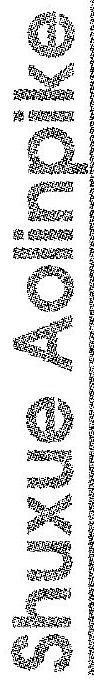
\includegraphics[max width=\textwidth, center]{2024_10_30_21385cc68d0979b6f3f8g-001}\\
初中卷\\
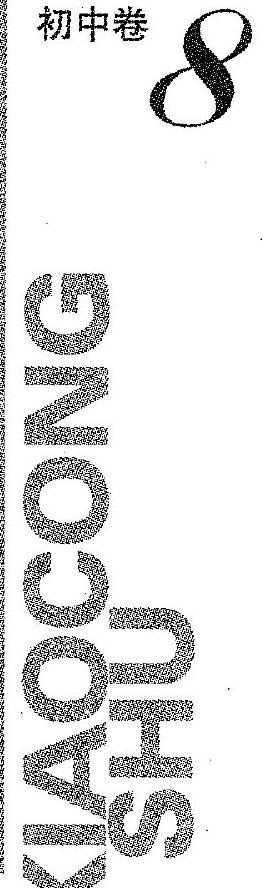
\includegraphics[max width=\textwidth, center]{2024_10_30_21385cc68d0979b6f3f8g-001(1)}

初中数学竞赛中的\\
解题方法与策略



\section{数学奥林匹克小丛书(第二版) 编委会}
冯志刚 第53届IMO中国队副领队、上海中学特级教师

\begin{center}
\begin{tabular}{|c|c|}
\hline
葛 军 & 博士、中国数学奥林匹克高级教练、南京师范大学副教授江苏省中学数学教学研究会副理事长 \\
\hline
冷岗松 & 国家集训队教练、上海大学教授、博士生导师 \\
\hline
李胜宏 & 第44届1MO中国队领队、浙江大学教授、博士生导师 \\
\hline
李伟固 & 中国数学奥林匹克委员会委员、国家集训队教练北京大学教授、博士生导师 \\
\hline
刘诗雄 & 华南师范大学中山附属中学校长、中学数学特级教师 \\
\hline
倪 明 & 华东师范大学出版社教辅分社社长、编审 \\
\hline
单 墫 & 第30、31届 MO 中国队领队、南京师范大学教授、博士生导师 \\
\hline
吴建平 & 中国数学会普及工作委员会主任、中国数学奥林匹克委员会副主席 \\
\hline
熊 斌 & \begin{tabular}{l}
第46、49、51、52、53届IMO中国队领队 \\
中国数学奥林匹克委员会委员、华东师范大学教授、博士生导师 \\
\end{tabular} \\
\hline
余红兵 & 中国数学奥林匹克委员会委员、国家集训队教练苏州大学教授、博士生导师 \\
\hline
\end{tabular}
\end{center}

朱华伟 中国教育数学学会常务副理事长、国家集训队教练广州大学软件所所长、研究员

\section{总}
\begin{center}
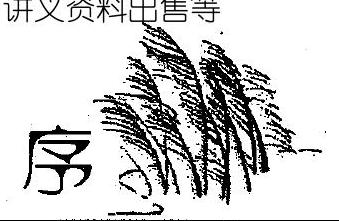
\includegraphics[max width=\textwidth]{2024_10_30_21385cc68d0979b6f3f8g-003}
\end{center}

数学竞赛像其他竞赛活动一样,是青少年学生的一种智力竞赛。在类似的以基础科学为竞赛内容的智力竞赛活动中,数学竞赛的历史最悠久、国际性强,影响也最大。我国于1956年开始举行数学竞赛,当时最有威望的著名数学家华罗庚、苏步青、江泽涵等都积极参加领导和组织竞赛活动,并组织出版了一系列青少年数学读物,激励了一大批青年学生立志从事科学事业。我国于1986年起参加国际数学奥林匹克,多次获得团体总分第一,并于1990年在北京成功地举办了第 31 届国际数学奥林匹克,这标志着我国数学竞赛水平在国际上居领先地位,为各国科学家与教育家所瞩目。

我国数学竞赛活动表明,凡是开展好的地区和单位,都能大大激发学生的学习数学的兴趣,有利于培养创造性思维,提高学生的学习效率。这项竟赛活动,将健康的竞争机制引进数学教学过程中,有利于选拔人才。由数学竞赛选拔的优胜者,既有踏实广泛的数学基础,又有刻苦钻研、科学的学习方法,其中的不少青年学生将来会成为出色的科学工作者。在美国,数学竟赛的优胜者中后来成名如米尔诺(J. W. Milnor)、芒福德(D. B. Mumford)、奎伦 (D. Quillen)等都是菲尔兹数学奖的获得者;在波兰,著名数论专家辛哲尔 (A. Schinzel)学生时代是一位数学竞赛优胜者;在匈牙利,著名数学家费叶尔 (L. Fejér)、里斯(M. Riesz)、舍贵(G. Szegö)、哈尔(A. Haar)、拉多 (T. Radó)等都曾是数学竞赛获奖者。匈牙利是开展数学竞赛活动最早的国家,产生了同它的人口不成比例的许多大数学家!

在开展数学竞赛的活动同时,各学校能加强联系,彼此交流数学教学经验,从这种意义上来说,数学竞赛可能成为数学课程改革的"催化剂",成为培养优秀人才的有力措施。

不过,应当注意在数学竞赛活动中,注意普及与提高相结合,而且要以普及为主,使竞赛具有广泛的群众基础,否则难以持久。

当然,现在有些人过于关注数学竟赛的成绩,组织和参与都具有很强的功利目的,过分扩大数学竞赛的作用,这些都是不正确的,违背了开展数学竞赛活动的本意。这些缺点有其深层次的社会原因,需要逐步加以克服,不必因

\section{1}
为有某些缺点,就否定这项活动。\\
我十分高兴看到这套《数学奧林匹克小丛书》的正式出版。这套书,规模大、专题细。据我所知,这样的丛书还不多见。这套书不仅对数学竟赛中出现的常用方法作了阐述,而且对竞赛题作了精到的分析解答,不少出自作者自己的研究所得,是一套很好的数学竞赛专题教程,也是中小学生和教师的参考书。

这套小丛书的作者都是数学竞赛教学和研究人员,不少是国家集训队的教练和国家队的领队。他们为我国开展数学竟赛的活动和我国学生在 IMO上取得成绩、为国争光作出了贡献,为这套书尽早面世付出了艰辛的劳动。华东师大出版社在出版《奥数教程》和《走向 IMO 》等竞赛图书基础上,策划组织了这套丛书,花了不少心血。我非常感谢作者们和编辑们在这方面所做的工作,并衷心祝愿我国的数学竞赛活动开展得越来越好。\\
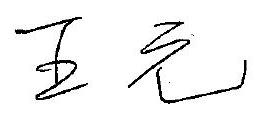
\includegraphics[max width=\textwidth, center]{2024_10_30_21385cc68d0979b6f3f8g-004}

\footnotetext{王元,著名数学家,中国科学院院士,曾任中国数学会理事长、中国数学奥林匹克委员会主席。
}\section{前}
数学竞赛问题的解决往往不是由拥有的知识量决定的,而需要透彻地理解问题的本质,充分发挥创造性,找到合适的方法才能一蹴而就。正是由于具有这样的特性,数学竟赛问题让许许多多聪明的中小学生着迷,数学竞赛活动受到广大学生的喜爱。

读小学的时候我们经常比谁"算得快",后来又以能帮助其他同学解决一些数学难题感到快乐,与"高手"们在一起讨论数学题非常开心,这都是数学本身的魅力带给我们的。数学问题的挑战性激发了很大的好奇心,这种源自内心的兴趣驱动,让很多学子爱上了数学、迷上了数学。

对比较聪明的那部分学生而言,更注重普适性的统编教林的内容很难让他们"吃饱",一些数学"难题"就成为了这些聪明学生乐于挑战的对象,他们从各种数学教辅书、问题集、大学教材、研究文章等资料中去寻找有味道的 "食物",老师们也经常从这些"难题"中挑选一些作为考题来甑别学生。我想这就是数学竞赛活动长期存在的源动力。

作为数学教育中不可或缺的重要部分,数学竞赛是中学生展示自已数学才华的最重要的平台,打开一张试卷、利用几张草稿纸和一支笔就能区分出学生数学水平之间的不同,这是最具公平性、有效性的方法,它是对人类智力最尊重也是成本最低的一项智力活动,国际数学奥林匹克活动吸引越来越多的国家或地区参加就是这个原因。

解题方法与策略在数学竞赛的学习中占有重要的地位,编写一本这样的小册子是希望起到"抛砖引玉"的作用。本书分为代数篇、几何篇、数论篇和组合篇,其中代数篇由于俊编写;几何篇由徐氾编写;数论篇由陈建豪编写;组合篇 $4.1 \sim 4.4$ 节由胡文备编写, $4.5 \sim 4.8$ 节由顾滨编写。鉴于作者水平有限,其中错误难免,敬请读者批评指正。

冯志刚\\
2012年1月1日

业务:初高中联赛班、培优班、美国高中数学、教师培训、机构教学产品研发、讲义资料出售等

业务:初高中联赛班、培优班、美国高中数学、教师培训、机构教学产品研发、讲义资料出售等

\section{符号说明}
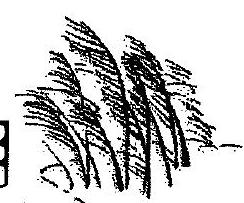
\includegraphics[max width=\textwidth, center]{2024_10_30_21385cc68d0979b6f3f8g-007}\\
[x]表示不超过 $x$ 的最大整数\\
$\sum$ 表示求和运算\\
$n !$ 表示 $1 \times 2 \times 3 \times \cdots \times n$\\
$n!$ ! 若正整数 $n$ 为奇数,则 $n!$ ! 表示 $n(n-2)(n-4) \cdots 3 \cdot 1$\\
若正整数 $n$ 为偶数, 则 $n$ !!表示 $n(n-2)(n-4) \cdots 4 \cdot 2$\\
$a \mid b$ 表示整数 $a$ 整除整数 $b$ 或者整数 $b$ 能够被整数 $a$ 整除\\
$d(m)$ 表示正整数 $m$ 的正因数的个数\\
$\pi(x)$ 表示正整数 $x$ 的不同素因数的个数\\
$a \equiv b(\bmod m) \quad$ 表示整数 $a$ 与 $b$ 对模 $m$ 同余\\
$(a, b)$ 表示正整数 $a$ 与 $b$ 的最大公约数\\
$[a, b]$ 表示正整数 $a$ 与 $b$ 的最小公倍数\\
$\lceil x\rceil$ 表示不小于 $x$ 的最小整数\\
$\max \{a, b\}$ 表示实数 $a$ 与 $b$ 中较大的一个数\\
$\min \{a, b\}$ 表示实数 $a$ 与 $b$ 中较小的一个数

业务:初高中联赛班、培优班、美国高中数学、教师培训、机构教学产品研发、讲义资料出售等\\
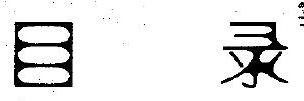
\includegraphics[max width=\textwidth, center]{2024_10_30_21385cc68d0979b6f3f8g-009}

\section{第一一部分 代数篇}
\section{1 巧用平方差公式}
\begin{enumerate}
  \item 2 恰当换元
\end{enumerate}

7

\begin{enumerate}
  \item 3 利用判别式解题 12
  \item 4 试试韦达定理 17\\
I. 5 主元素方法 21
  \item 6 利用对称性处理 25
  \item 7 恰当放缩 29
\end{enumerate}

第二部分 几何篇\\
2.1 面积公式及其应用 35\\
2.2 平移、旋转与翻折 41\\
2.3 构造相似 48\\
2.4 利用圆的性质 55\\
2.5 利用代数方法处理几何问题 61

\section{第三部分 数论篇}
3.1 奇偶分析 71\\
3.2 素因数分析 76\\
3.3 选择合适的模 79

全国小学奥数群:221739457,全国初中奥数学生群:253736211,全国高中奥数学生群591782992全国初中奥数教练群112464128,全国高中奥数教练群195949359竞赛公众号:新浪微博@郑剑雄 微信:v136257437 QQ:136257437\\
业务:初高中联赛班、培优班、美国高中数学、教师培训、机构教学产品研发、讲义资料出售等\\
3.4 做出适当的估计

4.2 染色或赋值 94\\
4. 3 分类与枚举 99\\
4.4 递推和归纳 103\\
4.5 极端原理 107\\
4.6 从局部到整体 111\\
4.7 将命题一般化或特殊化 115\\
4.8 先猜后证 119

习题解答 123\\
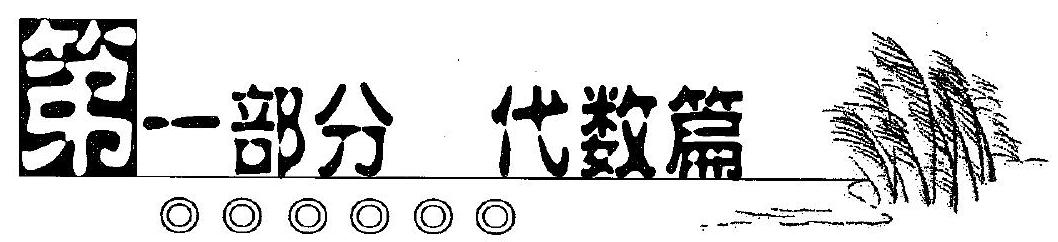
\includegraphics[max width=\textwidth, center]{2024_10_30_21385cc68d0979b6f3f8g-011}

代数是数学的基础分支,研究的是代数结构,强调的是各种变形和技巧。除了培养运算能丹,它还渗透在几何,数论,组合等各数学分支之中.学习代数的过程是艰辛而又漫长的,我们在追求结论正确的同时,也希望透过表象看到问题的本质,打下良好的数学基础。

业务:初高中联赛班、培优班、美国高中数学、教师培训、机构教学产品研发、讲义资料出售等

我们把公式 $(a+b)(a-b)=a^{2}-b^{2}$ 称为乘法公式中的平方差公式;反过来 $a^{2}-b^{2}=(a+b)(a-b)$ 称之为因式分解中的平方差公式。在一定条件下,把一个代数式变换成另一个与它恒等的代数式称为代数式恒等变形。平方差公式是代数式恒等变形中的重要公式之一,它在数值运算、代数式的化简与求值、不定方程(组)的解法、代数不等式的证明、一元二次方程的解法等方面都有广泛的运用。

例1 已知 $7^{12}-1$ 可被 40 至 50 之间的一个素数整除,这个素数是 ( ).\\
A. 41\\
B. 43\\
C. 47\\
D. 49

【解】用平方差公式作因式分解: $7^{12}-1=\left(7^{6}+1\right)\left(7^{6}-1\right)=\left(7^{2}+\right.$ 1) $\left(7^{4}-7^{2}+1\right)\left(7^{3}+1\right)\left(7^{3}-1\right)=50\left(7^{4}-7^{2}+1\right)(7+1)\left(7^{2}-7+1\right)(7-$ 1) $\left(7^{2}+7+1\right)=43 \cdot 48 \cdot 50 \cdot 57\left(7^{4}-7^{2}+1\right)$ ,而 $7^{4}-7^{2}+1=48 \cdot 49+1$不能被 41 ,49,47整除,故答案选 B.

【注】也可以用立方差公式分解 $7^{6}-1$ ,如果先用立方差公式,那么 $7^{6}-1=\left(7^{2}-1\right)\left(7^{4}+7^{2}+1\right)=48\left(7^{4}+7^{2}+1\right)$ ,而 $7^{4}+7^{2}+1$ 的分解可以通过拆项完成,具体分解如下:\\
\begin{align*}
\begin{aligned}
7^{4}+7^{2}+1 & =7^{4}+2 \cdot 7^{2}+1-7^{2} \\
& =\left(7^{2}+1\right)^{2}-7^{2} \\
& =\left(7^{2}+7+1\right)\left(7^{2}-7+1\right)
\end{aligned}
\end{align*}

例2 已知对任意大于 2 的正整数 $n, n^{5}-5 n^{3}+4 n$ 都是正整数 $m$ 的倍数,求 $m$ 的最大值。

【解】 $n^{5}-5 n^{3}+4 n=n\left(n^{4}-5 n^{2}+4\right)=n\left(n^{2}-4\right)\left(n^{2}-1\right)$\\
\begin{align*}
=n(n-2)(n+2)(n-1)(n+1)
\end{align*}

因为 $n(n-2)(n+2)(n-1)(n+1)$ 是五个连续正整数的乘积,所以它是 $5!$ 的倍数,又当 $n=3$ 时,原式 $=120$ ,故 $m$ 的最大值是 120 。

【注】这里用到了一个数论中的结论:连续的 5 个正整数的乘积是 5 !

的倍数,事实上,连续的 5 个正整数中必有 1 个 5 的倍数, 2 个 2 的倍数(其中一个为 4 的倍数), 1 个 3 的倍数。

顺便提一句,也可以利用组合数公式来证明连续 $n$ 个正整数的乘积是 $n$ !的倍数,这是因为由 $\mathrm{C}_{m}^{n}=\frac{m(m-1)(m-2) \cdots(m-n+1)}{n!}$ 可知连续的 $n$ 正整数乘积 $m(m-1)(m-2) \cdots(m-n+1)=n!C_{m}^{n}$ ,从而结论成立。

例3 计算: $\frac{\left(2^{4}+\frac{1}{4}\right)\left(4^{4}+\frac{1}{4}\right)\left(6^{4}+\frac{1}{4}\right)\left(8^{4}+\frac{1}{4}\right)\left(10^{4}+\frac{1}{4}\right)}{\left(1^{4}+\frac{1}{4}\right)\left(3^{4}+\frac{1}{4}\right)\left(5^{4}+\frac{1}{4}\right)\left(7^{4}+\frac{1}{4}\right)\left(9^{4}+\frac{1}{4}\right)}$.\\
【分析】由于括号内的每一个式子代数结构都相同,因此考虑用 $x^{4}+\frac{1}{4}$来代替,再进行因式分解后找出规律。

【解】 因为 $x^{4}+\frac{1}{4}=x^{4}+x^{2}+\frac{1}{4}-x^{2}=\left(x^{2}+\frac{1}{2}\right)^{2}-x^{2}$\\
\begin{align*}
\begin{aligned}
& =\left(x^{2}-x+\frac{1}{2}\right)\left(x^{2}+x+\frac{1}{2}\right) \\
& =\left[\left(x-\frac{1}{2}\right)^{2}+\frac{1}{4}\right]\left[\left(x+\frac{1}{2}\right)^{2}+\frac{1}{4}\right]
\end{aligned}
\end{align*}

004所以,原式 $=\left\{\left[\left(\frac{3}{2}\right)^{2}+\frac{1}{4}\right]\left[\left(\frac{5}{2}\right)^{2}+\frac{1}{4}\right]\left[\left(\frac{7}{2}\right)^{2}+\frac{1}{4}\right]\left[\left(\frac{9}{2}\right)^{2}+\frac{1}{4}\right] \cdots\right.$\\
\begin{align*}
\begin{aligned}
& {\left.\left[\left(\frac{19}{2}\right)^{2}+\frac{1}{4}\right]\left[\left(\frac{21}{2}\right)^{2}+\frac{1}{4}\right]\right\} \cdot\left\{\left[\left(\frac{1}{2}\right)^{2}+\frac{1}{4}\right]\left[\left(\frac{3}{2}\right)^{2}+\frac{1}{4}\right]\right.} \\
& {\left.\left[\left(\frac{5}{2}\right)^{2}+\frac{1}{4}\right]\left[\left(\frac{7}{2}\right)^{2}+\frac{1}{4}\right] \cdots\left[\left(\frac{17}{2}\right)^{2}+\frac{1}{4}\right]\left[\left(\frac{19}{2}\right)^{2}+\frac{1}{4}\right]\right\}^{-1} } \\
= & 221 .
\end{aligned}
\end{align*}

例4 若 $a$ 是非负整数,则 $a^{4}-3 a^{2}+9$ 是合数还是素数?\\
【解】由于 $a^{4}-3 a^{2}+9=\left(a^{2}+3\right)^{2}-(3 a)^{2}=\left(a^{2}-3 a+3\right)\left(a^{2}+3 a+\right.$ 3),下面对 $a$ 讨论:

当 $a=0$ 时,原式 $=9$ ,是一个合数;\\
当 $a=1$ 时,原式 $=7$ ,是一个素数;\\
当 $a=2$ 时,原式 $=13$ ,是一个素数;\\
当 $a>2$ 时,因 $a^{2}-3 a+3$ 与 $a^{2}+3 a+3$ 都是大于 1 的整数,故原式是一个合数。

综上所述,当 $a=0$ 或 $a>2$ 时, $a^{4}-3 a^{2}+9$ 是合数;当 $a=1$ 或 2 时, $a^{4}-$ $3 a^{2}+9$ 是素数。

【注】在将原式分解成 $\left(a^{2}-3 a+3\right)\left(a^{2}+3 a+3\right)$ 后,不能轻易下结论说

它就是个合数,因为要保证 $a^{2}-3 a+3$ 与 $a^{2}+3 a+3$ 都大于 1 才能是合数。\\
通过运用平方差公式进行因式分解的训练,可以使我们的观察能力、运算能力、变形能力、逻辑思维能力得到锻炼与提高,而在条件中能否找出或构造出 $a^{2}-b^{2}$ 的形式,然后用平方差公式进行分解成为解题的关键。

例5 求证:若 $n$ 是正整数,则存在无穷多个正整数 $k$ ,使得 $n^{4}+k$ 是合数。\\
【证明】令 $k=4 a^{4}$ ( $a$ 为正整数),则\\
\begin{align*}
\begin{aligned}
n^{4}+k & =n^{4}+4 a^{2} n^{2}+4 a^{4}-4 a^{2} n^{2}=\left(n^{2}+2 a^{2}\right)^{2}-(2 a n)^{2} \\
& =\left(n^{2}+2 a n+2 a^{2}\right)\left(n^{2}-2 a n+2 a^{2}\right)
\end{aligned}
\end{align*}

当 $a \geqslant 2$ 时, $n^{2}+2 a n+2 a^{2}$ 与 $n^{2}-2 a n+2 a^{2}$ 都是大于 1 的正整数。因为 $a$ 有无穷多个,故存在无穷多个 $k$ ,使得 $n^{4}+k$ 是合数。

【注】本题的关键在于构造 $k=4 a^{4}$ ,这用到了本章节例题 3 的代数形式。\\
例6 对于不超过 50 的正整数 $n$ ,满足:恰有一对非负整数 $(a, b)$ ,使得 $a^{2}-b^{2}=n$ ,试求满足条件的 $n$ 的数目。

【解】由于 $n=(a+b)(a-b)$ ,且 $a+b$ 与 $a-b$ 同奇偶,所以 $n \neq 2(\bmod 4)$ 。\\
(1)当 $n$ 为奇素数时,仅有一对 $(a, b)=\left(\frac{n+1}{2}, \frac{n-1}{2}\right)$ 满足条件;\\
(2)当 $n$ 为奇合数时,不妨设 $n=u v(u \geqslant v>1, u, v$ 为奇数),那么至少有 2 组非负整数解 $(a, b)=\left(\frac{n+1}{2}, \frac{n-1}{2}\right)$ 或 $\left(\frac{u+v}{2}, \frac{u-v}{2}\right)$ ,不满足题意,因此奇数中满足题意的共有:\\
$1,3,5,7,11,13,17,19,23,29,31,37,41,43,47$ 共计 15 个;\\
(3)当 $4 \mid n$ 时,如果 $\frac{n}{4}$ 为合数,至少有 2 组非负整数解,也不满足题意。因此偶数中满足条件的为 $4,8,12,20,28,44$ 共 6 个.

综上所述,一共有 21 个正整数 $n$ 满足题意。\\
【注】本题如果一开始直接枚举容易产生错误,约束适当的范围再进行枚举是关键。

例7 试求关于 $m, n$ 的不定方程 $m^{2}-1=p^{2}\left(n^{2}-1\right)$ 的所有正整数解,其中 $p$ 为素数。

【解】因为 $(m-1)(m+1)=p^{2}\left(n^{2}-1\right)$ ,下面按照 $p$ 作分类讨论:\\
(1)若 $p$ 为奇素数,则 $p^{2} \mid m-1$ 或 $p^{2} \mid m+1$ 。\\
若 $p^{2} \mid m-1$ ,设 $m=k p^{2}+1$ ( $k$ 为非负整数),则 $n^{2}=k^{2} p^{2}+2 k+1$ ,但是\\
\begin{align*}
k^{2} p^{2}<k^{2} p^{2}+2 k+1 \leqslant(k p+1)^{2}
\end{align*}

业务:初高中联赛班、培优班、美国高中数学、教师培训、机构教学产品研发、讲义资料出售等\\
从而 $k=0$, 进而 $m=n=1$;\\
若 $p^{2} \mid m+1$, 设 $m=k p^{2}-1$ ( $k$ 为正整数), 则 $n^{2}=k^{2} p^{2}-2 k+1$, 但是\\
\begin{align*}
(k p-1)^{2}<k^{2} p^{2}-2 k+1<k^{2} p^{2},
\end{align*}

矛盾!\\
(2) 若 $p$ 为 2 , 则 $2|m-1,2| m+1$, 设 $m=2 k-1$ ( $k$ 为正整数), 那么\\
\begin{align*}
n^{2}=k(k-1)+1=k^{2}-k+1 ;
\end{align*}

但是 $(k-1)^{2}<k^{2}-k+1 \leqslant k^{2}$, 故 $k=1$, 进而 $m=1$, 由此可得 $n=1$.\\
综上所述, $m=n=1$ 。\\
【注】本题的因式分解体现了处理整除时候常见的转成两边均是乘积式的模式,并且利用了两个相邻平方数之间没有平方数这一个性质,通过不等式控制,实现了论证。

\section{练 习 1.1}
들 计算: $\left(1-\frac{1}{2^{2}}\right)\left(1-\frac{1}{3^{2}}\right) \cdots\left(1-\frac{1}{2011^{2}}\right)$.\\
2 已知: $a^{2}-b^{2}=1+\sqrt{2}, b^{2}-c^{2}=1-\sqrt{2}$, 求 $a^{4}+b^{4}+c^{4}-a^{2} b^{2}-b^{2} c^{2}-$ $c^{2} a^{2}$ 的值。\\
证明:存在无穷多个完全平方数,它们无论对怎样的素数 $p$ 及怎样的正整数 $n 、 k$ ,都不能表示成 $p+n^{2 k}$ 的形式。\\
4 证明:对每个正整数 $n$ ,均存在正整数 $m$ ,使得:\\
\begin{align*}
(1+\sqrt{2})^{n}=\sqrt{m}+\sqrt{m+1}
\end{align*}

5试确定实数 $a 、 b 、 c$ 的值, 使得对任何正整数 $n$,\\
\begin{align*}
\sqrt{n}=\sum_{k=0}^{n-1} \sqrt[3]{\sqrt{a k^{3}+b k^{2}+c k+1}-\sqrt{a k^{3}+b k^{2}+c k}}
\end{align*}

恒成立。

业务:初高中联赛班、培优班、美国高中数学、教师培训、机构教学产品研发、讲义资料出售等\\
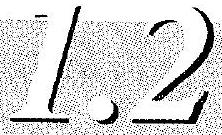
\includegraphics[max width=\textwidth, center]{2024_10_30_21385cc68d0979b6f3f8g-017}

一些看上去很复杂的代数式,通过观察与比较,如果可以发现相同或相似之处,此时可以用另一个变量来代替较复杂的代数式,从而起到简化计算的目的,这种方法叫做换元法,它大量运用于计算、化简、解方程、证明题中。

例1 计算: $\sqrt{2009 \times 2010 \times 2011 \times 2012+1}$ 。\\
【解】令 $n=2010$, 则\\
原式 $=\sqrt{(n-1) n(n+1)(n+2)+1}=\sqrt{\left(n^{2}+n\right)^{2}-2\left(n^{2}+n\right)+1}$\\
\begin{align*}
=n^{2}+n-1
\end{align*}

因为 $n=2010$ ,所以原式 $=4042109$ 。\\
【注】运用换元法可以使计算显得简洁。\\
例2 比较 $\sqrt{1+\sqrt{1+\sqrt{1+\cdots}}}$ 与 $1+\frac{1}{1+\frac{1}{1+\cdots}}$ 的大小。\\
【解】令 $\sqrt{1+\sqrt{1+\sqrt{1+\cdots}}}=M, 1+\frac{1}{1+\frac{1}{1+\cdots}}=N$, 则 $M=$ $\sqrt{1+M}, N=1+\frac{1}{N}$, 所以, $M^{2}-M-1=0, N^{2}-N-1=0$, 因为 $M>0$, $N>0$ ,所以 $M=N=\frac{1+\sqrt{5}}{2}$ 。

【注】在循环算式的计算和化简中经常采用本例中的处理方法.\\
例3 解方程组 $\left\{\begin{array}{l}\sqrt{x+\frac{1}{y}}-\sqrt{x+y-3}=\sqrt{3}, \\ 2 x+y+\frac{1}{y}=6 .\end{array}\right.$\\
【解】设 $\sqrt{x+\frac{1}{y}}=u, \sqrt{x+y-3}=v(u>0, v \geqslant 0$ ,且 $u>v)$ ,则原方 程 组 可 化 为 $\left\{\begin{array}{l}u-v=\sqrt{3}, \\ u^{2}+v^{2}=3,\end{array}\right.$ 解得 $\left\{\begin{array}{l}u=\sqrt{3}, \\ v=0 .\end{array}\right.$ 代入原方程组得

\section{厦门郑剑雄高中数学竞赛系列}
全国小学奥数群:221739457,全国初中奥数学生群:253736211,全国高中奥数学生群591782992\\
全国初中奥数教练群112464128,全国高中奥数教练群195949359\\
竞赛公众号:新浪微博@郑剑雄 微信:v136257437.QQ:136257437\\
业务:初高中联赛班、培优班、美国高中数学、教师培训、机构教学产品研发、讲义资料出售等\\
$\left\{\begin{array}{l}x+\frac{1}{y}=3, \\ x+y-3=0,\end{array}\right.$ 解得 $\left\{\begin{array}{l}x=2, \\ y=1\end{array}\right.$ 或 $\left\{\begin{array}{l}x=4, \\ y=-1 .\end{array}\right.$ 经检验, 原方程组的解为 $\left\{\begin{array}{l}x=2, \\ y=1\end{array}\right.$ 或 $\left\{\begin{array}{l}x=4, \\ y=-1 .\end{array}\right.$

【注】分式方程(组)和无理方程(组)最后要检验是否为增根。\\
例4 已知: $(y-z)^{2}+(z-x)^{2}+(x-y)^{2}=(y+z-2 x)^{2}+(z+x-$ $2 y)^{2}+(x+y-2 z)^{2}$, 试求: $\frac{(y z+1)(z x+1)(x y+1)}{\left(x^{2}+1\right)\left(y^{2}+1\right)\left(z^{2}+1\right)}$ 的值.

【解】令 $a=x-y, b=y-z, c=z-x$, 则条件转化为\\
\begin{align*}
a^{2}+b^{2}+c^{2}=(c-a)^{2}+(a-b)^{2}+(b-c)^{2},
\end{align*}

化简得\\
\begin{align*}
a^{2}+b^{2}+c^{2}-2 a b-2 b c-2 c a=0 .
\end{align*}

又\\
\begin{align*}
a+b+c=(x-y)+(y-z)+(z-x)=0,
\end{align*}

所以\\
\begin{align*}
(a+b+c)^{2}=a^{2}+b^{2}+c^{2}+2 a b+2 b c+2 c a=0,
\end{align*}

由 (1) + (2) 得 $a^{2}+b^{2}+c^{2}=0$, 故 $a=b=c=0$, 即\\
\begin{align*}
x-y=y-z=z-x=0,
\end{align*}

所以, $x=y=z$ ,原式 $=\frac{\left(x^{2}+1\right)\left(y^{2}+1\right)\left(z^{2}+1\right)}{\left(x^{2}+1\right)\left(y^{2}+1\right)\left(z^{2}+1\right)}=1$ 。\\
【注】换元法更能够体现问题的代数结构,突显出问题的实质。\\
例5 若 $m$ 是整数,且 $m \neq 0$ ,求证: $\frac{\sqrt[3]{2-\sqrt{5}}+\sqrt[3]{2+\sqrt{5}}}{m}$ 是有理数。\\
【证明】令 $x=\sqrt[3]{2+\sqrt{5}}, y=\sqrt[3]{2-\sqrt{5}}$, 则 $x^{3}+y^{3}=4$, 且 $x y=-1$,从而\\
\begin{align*}
x^{3}+y^{3}=(x+y)^{3}-3 x y(x+y)=4,
\end{align*}

进而\\
\begin{align*}
(x+y)^{3}-1+3(x+y)-3=0,
\end{align*}

即 $(x+y-1)\left[(x+y)^{2}+(x+y)+4\right]=0$, 又由于\\
\begin{align*}
(x+y)^{2}+(x+y)+4=\left(x+y+\frac{1}{2}\right)^{2}+\frac{15}{4}>0
\end{align*}

所以 $x+y-1=0, x+y=1$, 因为 $m$ 是整数且 $m \neq 0$, 所以

业务:初高中联赛班、培优班、美国高中数学、教师培训、机构教学产品研发、讲义资料出售等\\
\begin{align*}
\frac{\sqrt[3]{2-\sqrt{5}}+\sqrt[3]{2+\sqrt{5}}}{m}=\frac{1}{m}
\end{align*}

是有理数。\\
【注】此题运用换元法,结合 $x^{3}+y^{3}=4$ ,且 $x y=-1$ ,可以比较方便地进行等式的变形,以达到计算 $x+y$ 的目的。

例 6 解方程 $\sqrt[3]{45+x}+\sqrt[3]{16-x}=1$ 。\\
【解】设 $u=\sqrt[3]{45+x}, v=\sqrt[3]{16-x}$, 则 $\left\{\begin{array}{l}u+v=1, \\ u^{3}+v^{3}=61 .\end{array}\right.$\\
又 $u^{3}+v^{3}=(u+v)^{3}-3 u v(u+v)$ ,所以 $61=1-3 u v$ ,得 $u v=-20$ ,因此, $u , v$ 是方程 $y^{2}-y-20=0$ 的两根,解得 $y_{1}=5, y_{2}=-4$ ,即 $\sqrt[3]{45+x}=5$ 或 -4 ,解得 $x_{1}=-109 , x_{2}=80$ ,经检验, $x_{1}=-109 , x_{2}=80$ 都是原方程的根。

【注】此题的另一种解法如下:\\
令 $a=\sqrt[3]{45+x}, b=\sqrt[3]{16-x}, c=\sqrt[3]{-1}$ ,则 $a+b+c=0$ 。故\\
\begin{align*}
a^{3}+b^{3}+c^{3}-3 a b c=(a+b+c)\left(a^{2}+b^{2}+c^{2}-a b-b c-c a\right)=0
\end{align*}

即\\
\begin{align*}
45+x+16-x-1+3 \sqrt[3]{45+x} \cdot \sqrt[3]{16-x}=0
\end{align*}

化简得 $\sqrt[3]{(45+x)(16-x)}=-20$ ,解得 $x_{1}=-109, x_{2}=80$ 。\\
经检验, $x_{1}=-109, x_{2}=80$ 都是原方程的根。\\
【注】换元法经常需要和一些公式合起来用,所以考察代数式经过换元后可以适用哪个公式成为解题的关键,这需要对公式十分熟练地运用。

例7 解方程 $\left(x+2+\sqrt{x^{2}+4 x+3}\right)^{5}-32\left(x+2-\sqrt{x^{2}+4 x+3}\right)^{5}=$ 31.

【解】令 $a=x+2, b=\sqrt{x^{2}+4 x+3}$ ,则\\
\begin{align*}
\left\{\begin{array}{l}
(a+b)^{5}-32(a-b)^{5}=31 \\
a^{2}-b^{2}=1
\end{array}\right.
\end{align*}

由 (2) 知 $(a+b)(a-b)=1$ ,代人 (1) 得 $\left(\frac{1}{a-b}\right)^{5}-32(a-b)^{5}-31=0$ , $32(a-b)^{10}+31(a-b)^{5}-1=0$, 即 $\left[32(a-b)^{5}-1\right]\left[(a-b)^{5}+1\right]=0$,故 $a-b=\frac{1}{2}$ 或 $a-b=-1$, 分别代入 (2) 得 $\left\{\begin{array}{l}a+b=2, \\ a-b=\frac{1}{2}\end{array}\right.$ 或 $\left\{\begin{array}{l}a+b=-1, \\ a-b=-1,\end{array}\right.$ 得 $a=$ $\frac{5}{4}$ 或 -1 ,故 $x_{1}=-\frac{3}{4}, x_{2}=-3$ ,经检验, $x_{1}=-\frac{3}{4}, x_{2}=-3$ 都是原方程的解.

例8 求所有5元正整数组( $\left.x_{1}, x_{2}, x_{3}, x_{4}, x_{5}\right)$ ,使之满足 $x_{1}>x_{2}>$ $x_{3}>x_{4}>x_{5}$ ,且\\
\begin{align*}
\left[\frac{x_{1}+x_{2}}{3}\right]^{2}+\left[\frac{x_{2}+x_{3}}{3}\right]^{2}+\left[\frac{x_{3}+x_{4}}{3}\right]^{2}+\left[\frac{x_{4}+x_{5}}{3}\right]^{2}=38
\end{align*}

这里 $[x]$ 表示不超过 $x$ 的最大整数。\\
【解】 设 $a=\left[\frac{x_{1}+x_{2}}{3}\right], b=\left[\frac{x_{2}+x_{3}}{3}\right], c=\left[\frac{x_{3}+x_{4}}{3}\right], d=$ $\left[\frac{x_{4}+x_{5}}{3}\right]$, 则\\
\begin{align*}
a^{2}+b^{2}+c^{2}+d^{2}=38,
\end{align*}

由于 $x_{5} \geqslant 1, x_{4} \geqslant 2$, 所以 $a \geqslant b \geqslant c \geqslant d \geqslant 1$, 从而 $\frac{38}{4} \leqslant a^{2} \leqslant 35$, 即 $3<a<6$,下面讨论如下:\\
(1)若 $a=5$ ,则 $b^{2}+c^{2}+d^{2}=13$ ,经枚举可知不存在满足题意的正整数;\\
(2)若 $a=4$ ,则 $b^{2}+c^{2}+d^{2}=22$ ,经枚举可知满足题意的仅有 $b=3$ , $c=3, d=2$ ;

由于 $12 \leqslant x_{1}+x_{2}<15,9 \leqslant x_{2}+x_{3}<12,9 \leqslant x_{3}+x_{4}<12,6 \leqslant x_{4}+$ $x_{5}<9$, 从而根据 $x_{2} \geqslant x_{4}+2$ 可知必有 $x_{2}+x_{3}=11, x_{3}+x_{4}=9$ 且 $x_{2}=$ $x_{4}+2$ ,从而可得 $x_{2}=x_{3}+1, x_{3}=x_{4}+1$ ,因此 $x_{2}=6, x_{3}=5, x_{4}=4$ 。

于是 $7 \leqslant x_{1}<9,2 \leqslant x_{5}<4$ 。经检验可知,满足题意的 $\left(x_{1}, x_{2}, x_{3}\right.$ , $\left.x_{4}, x_{5}\right)$ 为 $(8,6,5,4,3),(8,6,5,4,2),(7,6,5,4,3),(7,6$, $5,4,2)$ 。

【注】利用整体换元实现对局部范围的约束是关键.

\section{练习 1.2}
1 已知 $a \geqslant \frac{1}{8}$, 求证: $\sqrt[3]{a+\frac{a+1}{3} \sqrt{\frac{8 a-1}{3}}}+\sqrt[3]{a-\frac{a+1}{3} \sqrt{\frac{8 a-1}{3}}}=1$.\\
2 计算: $\frac{\sum_{n=1}^{99} \sqrt{10+\sqrt{n}}}{\sum_{n=1}^{99} \sqrt{10-\sqrt{n}}}$ 的值.\\
经试求所有正整数 $n$ ,使得对于四个不同的正整数 $a 、 b 、 c 、 d$ ,在

\begin{verbatim}
夏门郑剑雄高中数学竞赛系列
\end{verbatim}

全国小学奥数群:221739457,全国初中奥数学生群:253736211,全国高中奥数学生群591782992全国初中奥数教练群112464128,全国高中奥数教练群195949359竞赛公众号:新浪微博@郑剑雄 微信:v136257437 QQ:136257437\\
业务:初高中联赛班、培优班、美国高中数学、教师培训、机构教学产品研发、讲义资料出售等\\
\begin{align*}
\frac{(a-c)(b-d)}{(b-c)(a-d)}, \frac{(b-c)(a-d)}{(a-c)(b-d)}, \frac{(a-b)(d-c)}{(a-d)(b-c)}, \frac{(a-c)(b-d)}{(a-b)(c-d)}
\end{align*}

中至少有 2 个等于 $n$.\\
4 证明:方程 $x^{2}+y^{5}=z^{3}$ 有无穷多组非零整数解。\\
㯺 设正整数 $k, n \geqslant 2$, 试求:\\
\begin{align*}
S(k, n)=\left[\frac{2^{n+1}+1}{2^{n-1}+1}\right]+\left[\frac{3^{n+1}+1}{3^{n-1}+1}\right]+\cdots+\left[\frac{k^{n+1}+1}{k^{n-1}+1}\right]
\end{align*}

的值。

关于 $x$ 的一元二次方程 $a x^{2}+b x+c=0(a \neq 0)$ ,我们用配方法可得 $a\left(x+\frac{b}{2 a}\right)^{2}=\frac{b^{2}-4 a c}{4 a}$, 故 $\left(x+\frac{b}{2 a}\right)^{2}=\frac{b^{2}-4 a c}{4 a^{2}}$ ,因为 $\left(x+\frac{b}{2 a}\right)^{2} \geqslant 0$ ,所以当 $b^{2}-4 a c \geqslant 0$ 时,原方程才有实数根。我们将 $b^{2}-4 a c$ 称为一元二次方程根的判别式,用符号" $\Delta$ "表示。具体来说,当 $b^{2}-4 a c>0$ 时,方程有两个不相等的实数根;当 $b^{2}-4 a c=0$ 时,方程有两个相等的实数根;当 $b^{2}-4 a c<0$ 时,方程没有实数根。

一元二次方程的根的判别式可以有两方面的作用:一是根据" $\Delta$ "的值来判断方程的实数根的情况;二是根据方程中实数根的情况,得出" $\Delta$ "的值,从而可以求出方程中的字母系数的值、系数之问的关系、字母的取值范围,进一步可以证明等式或不等式、求代数式的最值、求方程的整数解等等,它是实数根与系数之间的重要纽带。

例1 已知在关于 $x$ 的方程 $x^{2}+p_{1} x+q_{1}=0$ 与 $x^{2}+p_{2} x+q_{2}=0$ 中, $p_{1} p_{2}=2\left(q_{1}+q_{2}\right)$ ,求证:这两个方程至少有一个方程有实数根。

【证明】设这两个方程的判别式分别为 $\Delta_{1}$ 和 $\Delta_{2}$ ,则 $\Delta_{1}+\Delta_{2}=p_{1}^{2}-$ $4 q_{1}+p_{2}^{2}-4 q_{2}$ ,又 $p_{1} p_{2}=2\left(q_{1}+q_{2}\right)$ ,故 $\Delta_{1}+\Delta_{2}=p_{1}^{2}-2 p_{1} p_{2}+p_{2}^{2}=\left(p_{1}-\right.$ $\left.p_{2}\right)^{2} \geqslant 0$ ,所以 $\Delta_{1} \geqslant 0$ 与 $\Delta_{2} \geqslant 0$ 中至少有一个成立。因此,这两个方程至少有一个方程有实数根。

【注】 此题除了用到根的判别式外,还应用了平均数原理,即若 $P+$ $Q \geqslant R$ ,则 $P \geqslant \frac{R}{2}$ 与 $Q \geqslant \frac{R}{2}$ 中至少有一个成立。

例2 设 $a<b<c<d$ ,证明:对任意的实数 $t \neq-1$ ,关于 $x$ 的方程( $x-$ $a)(x-c)+t(x-b)(x-d)=0$ 都有两个不相等的实数根。

【证明】原方程可整理得\\
\begin{align*}
(1+t) x^{2}-[(a+c)+(b+d) t] x+(a c+b d t)=0
\end{align*}

因为 $t \neq-1$,\\
\begin{align*}
\begin{aligned}
\Delta_{1} & =[(a+c)+(b+d) t]^{2}-4(1+t)(a c+b d t) \\
& =(b-d)^{2} t^{2}+2[(a+c)(b+d)-2(a c+b d)] t+(a-c)^{2}
\end{aligned}
\end{align*}

由于 $b<d$ ,故 $(b-d)^{2}>0$ ,从而 (2) 式可看作关于 $t$ 的二次函数,图象开口向上,要证明 $\Delta_{1}>0$ ,只需要证明此二次函数与 $x$ 轴无交点,即关于 $t$ 的二次函数 (2) 的判别式 $\Delta_{2}<0$ 即可。\\
\begin{align*}
\text { 又 } \begin{aligned}
\Delta_{2} & =4[(a+c)(b+d)-2(a c+b d)]^{2}-4(b-d)^{2}(a-c)^{2} \\
& =16(a-d)(b-c)(a-b)(d-c)
\end{aligned}
\end{align*}

结合 $a<b<c<d$ ,故 $\Delta_{2}<0$ ,所以原方程有两个不相等的实数根。\\
【注】本题为了证明关于 $x$ 的方程有两个不相等的实数根,先将其转化为证明根的判别式 $\Delta_{1}>0$ ,又可将 $\Delta_{1}>0$ 转化为证明关于 $t$ 的二次函数与 $x$轴无交点,即 $\Delta_{2}<0$ 。连续两次化归给解题以明确的方向。

上面的例题是有关根据 $\Delta$ 的值来判断方程的实数根的情况,其实,还有大量已知方程根的情况,运用 $\Delta$ 的取值求方程中字母系数的值或取值范围,及字母系数之间的关系等类型的问题,下面分几种情况加以介绍:

\section{一、已知方程有实数根求系数的取值范围}
例3 已知方程 $x^{2}+4 a x-4 a+3=0,2 x^{2}-(4 a+1) x+2 a^{2}-1=0$中至少有一方程有实数根,求 $a$ 的取值范围。

【解】由题意得\\
\begin{align*}
\Delta_{1}=(4 a)^{2}+4(4 a-3) \geqslant 0
\end{align*}

解得 $a \geqslant \frac{1}{2}$ 或 $a \leqslant-\frac{3}{2}$ ;\\
\begin{align*}
\Delta_{2}=(4 a+1)^{2}-8\left(2 a^{2}-1\right) \geqslant 0
\end{align*}

解得 $a \geqslant-\frac{9}{8}$ ,所以, $a$ 的取值范围是 $a \geqslant-\frac{9}{8}$ 或 $a \leqslant-\frac{3}{2}$ 。\\
【注】本题也可以从反面考虑,即考虑两个方程均无实根的情形,请读者比较一下两种方法。

\section{二、已知整系数方程有有理根或整数根求系数或未知数的值}
对于整系数方程 $a x^{2}+b x+c=0(a \neq 0)$ ,若方程有有理根(或整数根),则其判别式一定是一个完全平方数,否则即为无理根。

例4 当 $x$ 为何有理数时,代数式 $9 x^{2}+23 x-2$ 的值恰好是两个连续正偶数的乘积?

【解】设两个连续偶数为 $k, k+2$ ( $k$ 为正偶数), 则

业务:初高中联赛班、培优班、美国高中数学、教师培训、机构教学产品研发、讲义资料出售等\\
\begin{align*}
9 x^{2}+23 x-2=k(k+2) \text {, 即 } 9 x^{2}+23 x-\left(k^{2}+2 k+2\right)=0 \text {. }
\end{align*}

因为 $x$ 是有理数,且此方程有有理根,所以它的判别式是完全平方数,令\\
\begin{align*}
\Delta=23^{2}+36\left(k^{2}+2 k+2\right)=565+36(k+1)^{2}=p^{2}(p \geqslant 0)
\end{align*}

从而 $p^{2}-36(k+1)^{2}=565$ ,即

故\\
\begin{align*}
\begin{aligned}
& \left\{\begin{array}{l}
p+6(k+1)=113 \\
p-6(k+1)=5
\end{array}\right. \\
& \left\{\begin{array}{l}
p+6(k+1)=565 \\
p-6(k+1)=1
\end{array}\right.
\end{aligned}
\end{align*}

解得 $\left\{\begin{array}{l}p=59, \\ k=8\end{array}\right.$ 或 $\left\{\begin{array}{l}p=283, \\ k=46 .\end{array}\right.$\\
代入方程 (1) 解得 $x_{1}=2, x_{2}=-\frac{41}{9}, x_{3}=-17, x_{4}=\frac{130}{9}$.\\
综上所述,当 $x_{1}=2, x_{2}=-\frac{41}{9}, x_{3}=-17, x_{4}=\frac{130}{9}$ 时,原代数式恰好为两个连续偶数 8 和 10 ,或 46 和 48 的乘积。

\section{三、运用判别式求代数式的最值}
例5 求 $\frac{3 x^{2}+6 x+5}{\frac{1}{2} x^{2}+x+1}$ 取最小值时的 $x$ 值.\\
【解】令 $y=\frac{3 x^{2}+6 x+5}{\frac{1}{2} x^{2}+x+1}$, 则\\
\begin{align*}
(y-6) x^{2}+2(y-6) x+2 y-10=0
\end{align*}

由题意得 $y \neq 6$ ,且 $\frac{1}{2} x^{2}+x+1=\frac{1}{2}(x+1)^{2}+\frac{1}{2}>0$ ,由于 $x$ 可取任何实数,所以方程 (1) 有实数根, $\Delta=4(y-6)^{2}-4(y-6)(2 y-10)=-4\left(y^{2}-\right.$ $10 y+24)=-4(y-5)^{2}+4 \geqslant 0$ ,解得 $4 \leqslant y \leqslant 6$ ,故 $4 \leqslant y<6$ 。将 $y=4$ 代入得 $x=-1$ ,故当 $x=-1$ 时,分式有最小值 4 。

【注】利用方程有解的必要条件,往往能够缩小范围,但要验证正确性。

\section{四、运用判别式解特殊的二元二次方程}
例 6 求方程 $5 x^{2}+6 x y+2 y^{2}-14 x-8 y+10=0$ 的实数解.

【解】将方程看作关于 $x$ 的一元二次方程,整理得\\
\begin{align*}
5 x^{2}+(6 y-14) x+2 y^{2}-8 y+10=0
\end{align*}

由题意得 $\Delta=(6 y-14)^{2}-20\left(2 y^{2}-8 y+10\right)=-4(y+1)^{2} \geqslant 0$, 所以\\
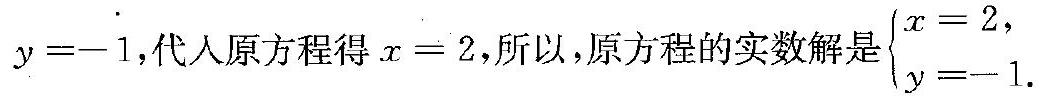
\includegraphics[max width=\textwidth, center]{2024_10_30_21385cc68d0979b6f3f8g-025}

【注】在求解特殊的二元二次方程时,常用主元法,具体内容将在本章 1.5 节加以介绍。当然,本题也可以将 $y$ 作为主元,读者不妨一试。

\section{五、构造一元一次方程有实根来证明等式或不等式}
例7 若 $a_{1}, a_{2}, \cdots, a_{n}, b_{1}, b_{2}, \cdots, b_{n}$ 都是实数,求证:\\
\begin{align*}
\left(a_{1}^{2}+a_{2}^{2}+\cdots+a_{n}^{2}\right)\left(b_{1}^{2}+b_{2}^{2}+\cdots+b_{n}^{2}\right) \geqslant\left(a_{1} b_{1}+a_{2} b_{2}+\cdots+a_{n} b_{n}\right)^{2}
\end{align*}

【分析】 直接展开后比较,处理起来很困难,若两边同乘以 4. 可以化为类似于 $4 a c \geqslant b^{2}$ 的形式,从而构造一元二次方程,利用根的判别式来证明。

【证明】(1)若 $a_{1}^{2}+a_{2}^{2}+\cdots+a_{n}^{2}=0$ ,则 $a_{1}=a_{2}=\cdots=a_{n}=0$ ,原不等式成立;\\
(2)若 $a_{1}^{2}+a_{2}^{2}+\cdots+a_{n}^{2} \neq 0$ ,构造二次函数\\
\begin{align*}
\begin{aligned}
y & =\left(a_{1}^{2}+a_{2}^{2}+\cdots+a_{n}^{2}\right) x^{2}-2\left(a_{1} b_{1}+a_{2} b_{2}+\cdots+a_{n} b_{n}\right) x+\left(b_{1}^{2}+b_{2}^{2}+\cdots+b_{n}^{2}\right) \\
& =\left(a_{1} x-b_{1}\right)^{2}+\left(a_{2} x-b_{2}\right)^{2}+\cdots+\left(a_{n} x-b_{n}\right)^{2} \geqslant 0,
\end{aligned}
\end{align*}

又 $a_{1}^{2}+a_{2}^{2}+\cdots+a_{n}^{2} \geqslant 0$ ,即二次函数开口向上,二次函数图象与 $x$ 轴无交点或只有一个交点, 故 $\Delta \leqslant 0$ 。即\\
\begin{align*}
\Delta=4\left(a_{1} b_{1}+a_{2} b_{2}+\cdots+a_{n} b_{n}\right)^{2}-4\left(a_{1}^{2}+a_{2}^{2}+\cdots+a_{n}^{2}\right)\left(b_{1}^{2}+b_{2}^{2}+\cdots+\right.
\end{align*}\\
$\left.b_{n}^{2}\right) \leqslant 0$,

所以,\\
\begin{align*}
\left(a_{1}^{2}+a_{2}^{2}+\cdots+a_{n}^{2}\right)\left(b_{1}^{2}+b_{2}^{2}+\cdots+b_{n}^{2}\right) \geqslant\left(a_{1} b_{1}+a_{2} b_{2}+\cdots+a_{n} b_{n}\right)^{2} .
\end{align*}

【注】所得的结论是著名的柯西(Cauchy)不等式,本题也可用向量方法证明。

例 8 已知函数 $f(x)=x^{2}+a x+b$, 其中 $a, b$ 为实数。若存在实数 $m$, 使得 $|f(m)| \leqslant \frac{1}{4}$ ,且 $|f(m+1)| \leqslant \frac{1}{4}$ ,试求: $\Delta=a^{2}-4 b$ 的最小值。

【解】 对任意实数 $x_{0}$ ,有\\
\begin{align*}
1=\left|\left(m+1-x_{0}\right)-\left(m-x_{0}\right)\right| \leqslant\left|m+1-x_{0}\right|+\left|m-x_{0}\right|,
\end{align*}

业务:初高中联赛班、培优班、美国高中数学、教师培训、机构教学产品研发、讲义资料出售等所以由抽屎原理可知 $\left|m+1-x_{0}\right|$ 与 $\left|m-x_{0}\right|$ 中必有一个不小于 $\frac{1}{2}$ 。

如果 $\Delta=a^{2}-4 b<0$, 那么 $f(m)=\left(m+\frac{a}{2}\right)^{2}-\frac{\Delta}{4}, f(m+1)=$ $\left(m+1+\frac{a}{2}\right)^{2}-\frac{\Delta}{4}$ 中必有一个大于 $\frac{1}{4}$, 这与题设矛盾, 所以 $\Delta \geqslant 0$.

又当 $a=-1, b=\frac{1}{4}$ 时, $|f(0)|=|f(1)|=\frac{1}{4}$, 且 $\Delta=0$, 所以 $\Delta=b^{2}-4 a c$的最小值为 0 。

\section{练 习 1.3}
1 试问:当 $m$ 是何整数时, $9 m^{2}+5 m+26$ 能够分解成两个连续正整数的乘积?\\
2 若 $a 、 b 、 c 、 d$ 、 $e$ 均为实数, 且满足 $a+b+c+d+e=8, a^{2}+b^{2}+c^{2}+$ $d^{2}+e^{2}=16$ ,求 $e$ 的最大值。\\
3设 $a 、 b 、 c$ 为 互 不 相 等 的 实 数,且满足关系式: $\left\{\begin{array}{l}b^{2}+c^{2}=2 a^{2}+16 a+14, \\ b c=a^{2}-4 a-5,\end{array}\right.$ 求 $a$ 的取值范围。\\
4 设正实数 $a 、 b$ ,二次三项式 $y^{2}-a y+b$ 的判别式 $\Delta$ 满足 $0<\Delta<2 a$ 。求证:不等式 $x^{4}-(a+1) x^{2}-\sqrt{\Delta} x+b \leqslant 0$ 的解集是总长度为 2 的两个区间的并集。\\
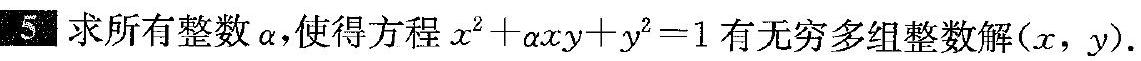
\includegraphics[max width=\textwidth, center]{2024_10_30_21385cc68d0979b6f3f8g-026}

业务:初高中联赛班、培优班、美国高中数学、教师培训、机构教学产品研发、讲义资料出售等

\section{试试韦达定理}
若方程 $a x^{2}+b x+c=0\left(a \neq 0, b^{2}-4 a c \geqslant 0\right)$ 有两个实根 $x_{1}, x_{2}$ ,则 $a x^{2}+$ $b x+c=a\left(x-x_{1}\right)\left(x-x_{2}\right)$ ,比较系数可得 $x_{1}+x_{2}=-\frac{b}{a}, x_{1} x_{2}=\frac{c}{a}$ ,这个性质揭示了一元二次方程的根与系数的关系,称之为韦达定理。运用这个定理可以不解方程确定两根之和,两根之积与系数之间的关系,从而可以求出关于两根的对称式的值,得出系数的取值或取值范围,构造新的一元二次方程等等,下面分几种情形来说明。

\section{一、由韦达定理求有关两根的代数式的值}
例1 已知 $s, t$ 是方程 $x^{2}-6 x+7=0$ 的两根,且 $s>t$ ,不解方程求 (1) $s-t$ ;(2) $\frac{2}{s}+3 t^{2}$ 的值。

【解】(1)由于 $s, t$ 是方程 $x^{2}-6 x+7=0$ 的两根,且 $s>t$ ,由韦达定理可得 $s+t=6, s t=7$, 所以 $s-t=\sqrt{(s-t)^{2}}=\sqrt{(s+t)^{2}-4 s t}=2 \sqrt{2}$.

【注】在题(2)中,由于 $\frac{2}{s}+3 t^{2}$ 是非对称式,因此采取"配对"的方法,引入与之对应的另一个非对称式 $-\frac{2}{t}+3 s^{2}$ ,从而达到整个式子为对称式的目的。计算它们的和与差,利用基本对称式 $x_{1}+x_{2}, x_{1} x_{2}$ ,运用韦达定理最后求出\\
\begin{align*}
\begin{gathered}
\text { (2) 令 } A=\frac{2}{s}+3 t^{2}, B=\frac{2}{t}+3 s^{2} \text {, 则 } \\
A+B=\frac{2}{s}+\frac{2}{t}+3\left(s^{2}+t^{2}\right)=\frac{2(s+t)}{s t}+3\left[(s+t)^{2}-2 s t\right]=\frac{474}{7}, \\
A-B=\frac{2}{s}-\frac{2}{t}+3\left(t^{2}-s^{2}\right)=\frac{2(t-s)}{s t}+3(t+s)(t-s)=-\frac{256 \sqrt{2}}{7} . \\
\text { 由 (1) }+ \text { (2) 得 } 2 A=\frac{474-256 \sqrt{2}}{7} \text {, 故 } A=\frac{2}{s}+3 t^{2}=\frac{237-128 \sqrt{2}}{7} .
\end{gathered}
\end{align*}

业务:初高中联赛班、培优班、美国高中数学、教师培训、机构教学产品研发、讲义资料出售等 $\frac{2}{s}+3 t^{2}$ 的值。

例2 设 $x_{1}, x_{2}$ 是方程 $2 x^{2}-4 m x+2 m^{2}+3 m-2=0$ 的两个实根,当 $m$为何值时, $x_{1}^{2}+x_{2}^{2}$ 有最小值,试求这个最小值。

【解】因为 $\Delta=16 m^{2}-8\left(2 m^{2}+3 m-2\right) \geqslant 0$ ,即 $-24 m+16 \geqslant 0$ ,解得 $m \leqslant \frac{2}{3}$, 又由题意得 $x_{1}+x_{2}=2 m, x_{1} x_{2}=\frac{2 m^{2}+3 m-2}{2}$, 故\\
\begin{align*}
x_{1}^{2}+x_{2}^{2}=\left(x_{1}+x_{2}\right)^{2}-2 x_{1} x_{2}=2 m^{2}-3 m+2=2\left(m-\frac{3}{4}\right)^{2}+\frac{7}{8}
\end{align*}

因 $m \leqslant \frac{2}{3}<\frac{3}{4}$, 所以当 $m=\frac{2}{3}$ 时, $x_{1}^{2}+x_{2}^{2}$ 有最小值 $2\left(\frac{2}{3}-\frac{3}{4}\right)^{2}+\frac{7}{8}=$ $\frac{8}{9}$.

【注】在运用韦达定理时,最容易忽视的条件是要在有实数根的前提下,本题也要防止出现当 $m=\frac{3}{4}$ 时, $x_{1}^{2}+x_{2}^{2}$ 有最小值 $\frac{7}{8}$ 的错误。

\section{二、由韦达定理构造方程来解题}
若 $x_{1}+x_{2}=p, x_{1} x_{2}=q$ ,则可构造方程 $x^{2}-p x+q=0$ (其两根为 $x_{1}$ , $x_{2}$ )来处理问题。

例3 解方程 $(2+\sqrt{3})^{x}+(2-\sqrt{3})^{x}=4$.\\
【分析】直接解方程比较难,观察到 $2+\sqrt{3}$ 与 $2-\sqrt{3}$ 互为倒数,可以得到 $(2+\sqrt{3})^{x} \cdot(2-\sqrt{3})^{x}=1$ ,再结合 $(2+\sqrt{3})^{x}+(2-\sqrt{3})^{x}=4$ ,可以构造一元二次方程用韦达定理来解题。

【解】因为 $(2+\sqrt{3})(2-\sqrt{3})=1$, 故 $(2+\sqrt{3})^{x} \cdot(2-\sqrt{3})^{x}=1$, 令\\
\begin{align*}
a=(2+\sqrt{3})^{x}, b=(2-\sqrt{3})^{x}
\end{align*}

则 $\left\{\begin{array}{l}a+b=4, \\ a b=1 .\end{array}\right.$ 解得 $\left\{\begin{array}{l}a=2+\sqrt{3}, \\ b=2-\sqrt{3}\end{array}\right.$ 或 $\left\{\begin{array}{l}a=2-\sqrt{3}, \\ b=2+\sqrt{3} .\end{array}\right.$\\
所以 $(2+\sqrt{3})^{x}=2+\sqrt{3}$ 或 $(2+\sqrt{3})^{x}=2-\sqrt{3}$, 解得 $x=1$ 或 $x=-1$.

\section{三、用韦达定理解有关一元二次方程的整数根的问题}
例4 设方程 $x^{2}-p x+q=0, x^{2}-q x+p=0$ 的根都是正整数,求正整数 $p, q$ 的值。

业务:初高中联赛班、培优班、美国高中数学、教师培训、机构教学产品研发、讲义资料出售等

【解】 设 $x^{2}-p x+q=0$ 的两根为 $x_{1}, x_{2} ; x^{2}-q x+p=0$ 的两根为 $x_{3}, x_{4}$ ,由韦达定理得 $x_{1}+x_{2}=p, x_{1} x_{2}=q, x_{3}+x_{4}=q, x_{3} x_{4}=p$ ,故\\
\begin{align*}
\left\{\begin{array}{l}
x_{1}+x_{2}=x_{3} x_{4} \\
x_{3}+x_{4}=x_{1} x_{2}
\end{array}\right.
\end{align*}

由(2)-(1)得 $x_{1} x_{2}-x_{1}-x_{2}+x_{3} x_{4}-x_{3}-x_{4}=0$ ,\\
即\\
\begin{align*}
\left(x_{1}-1\right)\left(x_{2}-1\right)+\left(x_{3}-1\right)\left(x_{4}-1\right)=2 .
\end{align*}

因为 $x_{1}, x_{2}, x_{3}, x_{4}$ 均为正整数,所以\\
$\left\{\begin{array}{l}\left(x_{1}-1\right)\left(x_{2}-1\right)=2, \\ \left(x_{3}-1\right)\left(x_{4}-1\right)=0\end{array}\right.$ 或 $\left\{\begin{array}{l}\left(x_{1}-1\right)\left(x_{2}-1\right)=1, \\ \left(x_{3}-1\right)\left(x_{4}-1\right)=1\end{array}\right.$ 或 $\left\{\begin{array}{l}\left(x_{1}-1\right)\left(x_{2}-1\right)=0, \\ \left(x_{3}-1\right)\left(x_{4}-1\right)=2 .\end{array}\right.$\\
解得 $\left\{\begin{array}{l}x_{1}+x_{2}=p=5, \\ x_{1} x_{2}=q=6\end{array}\right.$ 或 $\left\{\begin{array}{l}x_{1}+x_{2}=p=4, \\ x_{1} x_{2}=q=4\end{array}\right.$ 或 $\left\{\begin{array}{l}x_{3}+x_{4}=q=5, \\ x_{3} x_{4}=p=6 .\end{array}\right.$\\
所以, $\left\{\begin{array}{l}p=5, \\ q=6\end{array}\right.$ 或 $\left\{\begin{array}{l}p=4, \\ q=4\end{array}\right.$ 或 $\left\{\begin{array}{l}p=6, \\ q=5 .\end{array}\right.$\\
例 5 已知 $p, q$ 为整数,并且是关于 $x$ 的方程 $x^{2}-\frac{p^{2}+11}{9} x+\frac{15}{4}(p+$ $q)+16=0$ 的两根, 求 $p, q$ 的值.

【解】由韦达定理得 $\left\{\begin{array}{l}p+q=\frac{p^{2}+11}{9}, \\ p q=\frac{15}{4}(p+q)+16 .\end{array}\right.$\\
由 (1) 知 $p+q>0$ ,代人 (2) 得 $p q>0$ ,故 $p>0, q>0$ 。\\
由(2)得\\
\begin{align*}
16 p q=60(p+q)+16^{2}
\end{align*}

即\\
\begin{align*}
(4 p-15)(4 q-15)=481=1 \times 481=13 \times 37
\end{align*}

故 $\left\{\begin{array}{l}4 p-15=1, \\ 4 q-15=481\end{array}\right.$ 或 $\left\{\begin{array}{l}4 p-15=481, \\ 4 q-15=1\end{array}\right.$ 或 $\left\{\begin{array}{l}4 p-15=13, \\ 4 q-15=37\end{array}\right.$ 或 $\left\{\begin{array}{l}4 p-15=37, \\ 4 q-15=13 .\end{array}\right.$解得 $\left\{\begin{array}{l}p=4, \\ q=124\end{array}\right.$ 或 $\left\{\begin{array}{l}p=124, \\ q=4\end{array}\right.$ 或 $\left\{\begin{array}{l}p=7, \\ q=13\end{array}\right.$ 或 $\left\{\begin{array}{l}p=13, \\ q=7 .\end{array}\right.$

代入(1)得 $p^{2}=1141$ (舍去)或 $p^{2}=169$ ,所以 $p=13, q=7$ ,此时方程化为 $x^{2}-20 x+91=0$ ,它的两根为 13 和 7 。所以, $p=13, q=7$ 。

例 6 给定了 $n(n>1)$ 个二次三项式 $x^{2}-a_{1} x+b_{1}, \cdots, x^{2}-a_{n} x+b_{n}$ ,其中 $2 n$ 个实数 $a_{1}, \cdots, a_{n}, b_{1}, \cdots, b_{n}$ 互不相同。试问:是否可能每个多项式的根都是 $a_{1}, \cdots, a_{n}, b_{1}, \cdots, b_{n}$ 中的数?

【解】假设有这样的可能性,那么由于 $a_{1}, \cdots, a_{n}, b_{1}, \cdots, b_{n}$ 这 $2 n$ 个实数互不相同,它们构成了 $n$ 个二次三项式的所有根的全体,其中每个二次三项式均有两个根。假设 $\alpha_{i}, \beta_{i}$ 是二次方程 $x^{2}-a_{i} x+b_{i}=0$ 的两个根,则由韦达定理知 $a_{i}=\alpha_{i}+\beta_{i}, b_{i}=\alpha_{i} \beta_{i}$ ,既然 $n$ 个二次三项式的所有根的全体就是 $a_{1}, \cdots$ , $a_{n}, b_{1}, \cdots, b_{n}$ ,所以就有\\
\begin{align*}
\sum_{i=1}^{n} a_{i}=\sum_{i=1}^{n}\left(\alpha_{i}+\beta_{i}\right)=\sum_{i=1}^{n}\left(a_{i}+b_{i}\right)=\sum_{i=1}^{n} a_{i}+\sum_{i=1}^{n} b_{i} .
\end{align*}

因此 $\sum_{i=1}^{n} b_{i}=0$ 。另一方面, 有 $\alpha_{i}^{2}+\beta_{i}^{2}=\left(\alpha_{i}+\beta_{i}\right)^{2}-2 \alpha_{i} \beta_{i}=a_{i}^{2}-2 b_{i}$.\\
从而\\
\begin{align*}
\sum_{i=1}^{n}\left(a_{i}^{2}+b_{i}^{2}\right)=\sum_{i=1}^{n}\left(\alpha_{i}^{2}+\beta_{i}^{2}\right)=\sum_{i=1}^{n}\left(a_{i}^{2}-2 b_{i}\right)=\sum_{i=1}^{n} a_{i}^{2},
\end{align*}

这表明 $\sum_{i=1}^{n} b_{i}^{2}=0$ ,于是所有的 $b_{i}$ 都为 0 ,与题意相矛盾。从而本题的结论是否定的。

【注】这里通过韦达定理的过渡,实现了总体和与部分和在代数上的相互衔接。

\section{练 习1.4}
若 $a 、 b$ 为正整数,试问:关于 $x$ 的方程 $x^{2}-a b x+\frac{1}{2}(a+b)=0$ 是否有两个正整数解?\\
2 当 $a$ 为何值时,方程 $x^{2}+2 a x+2 a^{2}-1=0$ 至少有一个正根?\\
5若 $m$ 为负实数,求证:方程 $\frac{1}{x}+\frac{1}{x+m}+\frac{1}{x+m^{2}}=0$ 有两个符号相反的实数根,其中正根必小于 $-\frac{2}{3} m$ ,负根必大于 $-\frac{2}{3} m^{2}$ 。\\
4 已知:方程 $x^{2}+p x+q=0$ 的系数 $p$ 与 $q$ 被改变为新系数,新旧系数之间相差 0.001. 试问:新方程的较大根与旧方程较大根之间的差能否大于等于 1000 ?\\
5 欲 给定二次三项式 $f(x)=x^{2}+a x+b$ 。现已知方程 $f(f(x))=0$ 有 4 个不同的实根,其中有两个根的和等于 -1 . 证明: $b \leqslant-\frac{1}{4}$.

业务:初高中联赛班、培优班、美国高中数学、教师培训、机构教学产品研发、讲义资料出售等\\
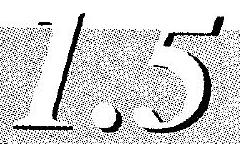
\includegraphics[max width=\textwidth, center]{2024_10_30_21385cc68d0979b6f3f8g-031}

\section{主元素方法}
当一个代数式中含有两个或两个以上变量时,通常采取适当的变形,确定其中的一个变量为主变量,从主变量的角度来解决问题,这种方法就称为主元素方法。

例1 求方程 $2 x^{2}+y^{2}-2 x y-4 x-30=0$ 的正整数解。\\
【解】原方程视为关于 $y$ 的二次方程:\\
\begin{align*}
y^{2}-2 x y+\left(2 x^{2}-4 x-30\right)=0
\end{align*}

则 $\Delta=4 x^{2}-4\left(2 x^{2}-4 x-30\right)=4\left[34-(x-2)^{2}\right]$ 是一个完全平方数,知 $(x-2)^{2}=9$ 或 25 ,由于 $x$ 为正整数,故 $x=5$ 或 7 。当 $x=5$ 时,原方程化为 $y^{2}-10 y=0$ ,解得 $y_{1}=10 , y_{2}=0$ ;当 $x=7$ 时,原方程化为 $y^{2}-14 y+40=$ 0 ,解得 $y_{1}=10, y_{2}=4$ 。所以,原方程的正整数解 $(x, y)$ 为 $(5,10),(7,10)$ , $(7,4)$.

【注】本题也可以 $x$ 为主元,读者不妨一试。\\
例2 若二次方程 $a x^{2}+2(2 a-1) x+4(a-3)=0$ 至少有一个整数根,求正整数 $a$ 的值。

【分析】本题可看作是关于 $x$ 的一元二次方程,根据根的判别式及求根公式,能求出正整数 $a$ 的值。再换一个角度看,若以 $a$ 为主元,把它变形为关于 $a$ 的一元一次方程,是不是也能解呢?

【解法一】由题意得 $\Delta=4(8 a+1)$ 是一个完全平方数,因 $8 a+1$ 是奇数,故它一定是奇数的平方,设 $8 a+1=(2 m+1)^{2}$ ( $m$ 为正整数),解得 $a=$ $\frac{1}{2} m(m+1)$ ,将 $a$ 的值代入原方程得 $x_{1}=-2+\frac{4}{m}, x_{2}=-2-\frac{4}{m+1}$ 。由于 $x_{1}, x_{2}$ 中至少有一个为整数,故 $m \mid 4$ 或 $(m+1) \mid 4$, 又 $m$ 为正整数, 因此 $m=$ $1,2,3,4$ ,解得 $a=1,3,6,10$ 。

【解法二】将原方程整理成关于 $a$ 的方程 $a=\frac{2 x+12}{(x+2)^{2}}(x \neq-2)$ ,因 $a$为正整数,故 $a=\frac{2 x+12}{(x+2)^{2}} \geqslant 1$ ,整理得 $x^{2}+2 x-8 \leqslant 0$ ,解得 $-4 \leqslant x \leqslant 2$ 。

又因为 $x$ 是整数, 故 $x=-4,-3,-2,0,1,2$, 分别代入得 $a=1,6,10,3$, $\frac{14}{9}, 1$ ,得 $a$ 的值为 $1,3,6,10$ 。

例 3 解方程 $x^{4}-2 \sqrt{3} x^{2}-x+3-\sqrt{3}=0$.\\
【分析】本题属于解高次方程, 并且系数 $\sqrt{3}$ 是无理数, 用因式分解方法很困难。仔细观察系数 $\sqrt{3}$ 和 3 ,发现 $3=(\sqrt{3})^{2}$ ,这就给我们一个思路:把 $\sqrt{3}$ 看作一个元。

【解】设 $\sqrt{3}=a$ ,则原方程化为 $x^{4}-2 a x^{2}-x+a^{2}-a=0$ ,整理为关于 $a$ 的方程,得 $a^{2}-\left(2 x^{2}+1\right) a+x^{4}-x=0$ ,因式分解得\\
\begin{align*}
\left[a-\left(x^{2}-x\right)\right]\left[a-\left(x^{2}+x+1\right)\right]=0,
\end{align*}

故 $a=x^{2}-x$ 或 $a=x^{2}+x+1$, 即 $x^{2}-x-\sqrt{3}=0$ 或 $x^{2}+x+1-\sqrt{3}=0$.\\
解得 $x=\frac{1 \pm \sqrt{1+4 \sqrt{3}}}{2}$ 或 $x=\frac{-1 \pm \sqrt{4 \sqrt{3}-3}}{2}$.\\
【注】这里我们突破了常规思维,把 $\sqrt{3}=a$ 看作一个主元,这种把某个常数作为主元的方法虽然不常用,但有时却非常有效。

例4 设 $a, b, c$ 为三个不同的非零实数,解关于 $x, y, z$ 的方程组:\\
\begin{align*}
\left\{\begin{array}{l}
\frac{x}{a^{3}}-\frac{y}{a^{2}}+\frac{z}{a}=1 \\
\frac{x}{b^{3}}-\frac{y}{b^{2}}+\frac{z}{b}=1 \\
\frac{x}{c^{3}}-\frac{y}{c^{2}}+\frac{z}{c}=1
\end{array}\right.
\end{align*}

【分析】解三元一次方程组,一般方法是消元、降次为一元一次方程。但是本题由于 $a, b, c$ 三个字母系数的存在,使得计算非常繁琐,但这三个方程非常有特点,方程的形式相似,不同的是方程中的系数由 $a$ 换为 $b, c$ ,能否转换思路,把 $a , b , c$ 看作主元,将 $x , y , z$ 看作系数呢?

【解】由题意得 $a, b, c$ 分别是关于 $t$ 的方程 $\frac{x}{t^{3}}-\frac{y}{t^{2}}+\frac{z}{t}=1$ 的三个不同实根,整理得 $t^{3}-z t^{2}+y t-x=0$ ,根据韦达定理得 $\left\{\begin{array}{l}x=a b c, \\ y=a b+b c+c a , \\ z=a+b+c\end{array}\right.$

例5 已知 $y=\left(2 x^{5}+2 x^{4}-53 x^{3}-57 x+54\right)^{2011}$, 求当 $x=\frac{1}{2}(\sqrt{111}-$

1)时的函数值.\\
【分析】 若直接将 $x=\frac{1}{2}(\sqrt{111}-1)$ 代入,必然很繁琐,适当变形得 $2 x+1=\sqrt{111}$ ,则 $2 x^{2}+2 x-55=0$ ,将 $t=2 x^{2}+2 x-55$ 作为主元,将原式化为 $t$ 的形式,然后计算,将会使计算简化。

【解】 因 $x=\frac{1}{2}(\sqrt{111}-1)$ ,故 $2 x+1=\sqrt{111}, 2 x^{2}+2 x-55=0$ ,而 $\left(2 x^{5}+2 x^{4}-53 x^{3}-57 x+54\right)$ 除以 $\left(2 x^{2}+2 x-55\right)$ 后所得的商式是 $x^{3}+$ $x-1$ ,余式为 -1 ,故 $y=\left[\left(2 x^{2}+2 x-55\right)\left(x^{3}+x-1\right)-1\right]^{2011}=-1$ 。

例 6 求使不等式 $x^{2}+p x>4 x+p-3$ 对满足 $0 \leqslant p \leqslant 4$ 的实数 $p$ 都成立的 $x$ 的取值范围。

【分析】 如果将不等式看作关于 $x$ 的函数 $f(x)=x^{2}+(p-4) x-p+$ $3>0$ 来解,由于已经知道 $p$ 的取值范围求 $x$ 的取值范围,而非已知 $x$ 的取值范围求 $p$ 的值。问题陷人僵局,换一个角度,以 $p$ 为主元呢?

【解】 原不等式即 $x^{2}+(x-1) p-4 x+3>0$ ,令 $f(p)=(x-1) p+x^{2}-$ $4 x+3$, 这是 $f$ 关于 $p$ 的一次函数,因为 $0 \leqslant p \leqslant 4$ ,由一次函数图象得 $f(p)>0$恒成立的条件是:\\
\begin{align*}
\left\{\begin{array} { l } 
{ f ( 0 ) > 0 , } \\
{ f ( 4 ) > 0 , }
\end{array} \text { 即 } \left\{\begin{array}{l}
x^{2}-4 x+3>0, \\
x^{2}-1>0,
\end{array}\right.\right.
\end{align*}

解得 $x>3$ 或 $x<-1$ 。\\
例7 设正整数 $x_{1}, x_{2}, x_{3}, x_{4}, x_{5}$ 满足 $x_{1}+x_{2}+x_{3}+x_{4}+x_{5}=$ $x_{1} x_{2} x_{3} x_{4} x_{5}$ ,求 $x_{5}$ 的最大值。

【解】由对称性,不妨设 $x_{1} \leqslant x_{2} \leqslant x_{3} \leqslant x_{4} \leqslant x_{5}, x_{1}, x_{2}, x_{3}, x_{4}, x_{5}$ 都是正整数,故\\
\begin{align*}
\begin{aligned}
1 & =\frac{1}{x_{1} x_{2} x_{3} x_{4}}+\frac{1}{x_{1} x_{2} x_{3} x_{5}}+\frac{1}{x_{1} x_{3} x_{4} x_{5}}+\frac{1}{x_{2} x_{3} x_{4} x_{5}}+\frac{1}{x_{1} x_{2} x_{4} x_{5}} \\
& \leqslant \frac{1}{x_{4}}+\frac{1}{x_{5}}+\frac{1}{x_{4} x_{5}}+\frac{1}{x_{4} x_{5}}+\frac{1}{x_{4} x_{5}}=\frac{3+x_{4}+x_{5}}{x_{4} x_{5}}
\end{aligned}
\end{align*}

所以 $x_{4} x_{5} \leqslant 3+x_{4}+x_{5}$, 即 $\left(x_{4}-1\right)\left(x_{5}-1\right) \leqslant 4$, 若 $x_{4}=1$, 则 $x_{1}=x_{2}=x_{3}=$ $x_{4}=1$ ,得 $x_{5}=4+x_{5}$ 无解,故 $x_{4}>1$ ,且为整数,因此 $x_{4}-1 \geqslant 1 , x_{5}-1 \leqslant 4$ , $x_{5} \leqslant 5$ 。 当 $x_{5}=5$ 时, $(1,1,1,2,5)$ 是适合已知条件的一组数,可见 $x_{5}$ 的最大值为 5 。

【注】此题有五个变量,利用排序,结合不等式和已知条件等式,将问题转化为以变量 $x_{5}$ 为主元的等式或不等式是解题的关键。

\section{练 1.5}
1固解方程组 $\left\{\begin{array}{l}x+y+z=3, \\ x^{2}+y^{2}+z^{2}=3, \\ x^{3}+y^{3}+z^{3}=3 .\end{array}\right.$\\
2 若 $F\left(\frac{1-x}{1+x}\right)=x$ ,试求 $F(-2-x)$ 的表达式。\\
龮设 $x, y, z$ 均为实数, 试求\\
\begin{align*}
f(x, y, z)=(x+y)^{2}+(y+z)^{2}+(x+z-2)^{2}+(x+y+z)^{2}
\end{align*}

的最小值。\\
4 若实数 $x 、 y$ 满足 $x-3 \sqrt{x+1}=3 \sqrt{y+2}-y$, 试求 $p=x+y$ 的最大值和最小值。\\
5 求满足下述条件的最小正实数 $k$ :对任意不小于 $k$ 的 4 个互不相同的实数 $a 、 b 、 c 、 d$ ,都存在一个排列 $p, q, r, s$ ,使得方程\\
\begin{align*}
\left(x^{2}+p x+q\right)\left(x^{2}+r x+s\right)=0
\end{align*}

有 4 个互不相同的实根。

在现实生活中,存在大量的对称的美,例如房屋、汽车、蝴蝶、篮球 $\cdots \cdots$ ,甚至人的身体也是对称的。在数学中也存在许多诸如对称式,对称方程,对称算法,对称图形等等,结构上的对称使得解题的任意性变得有序化、规则化。

例1 甲、乙两人在 $19 \times 19$ 的格子棋盘下棋,规则如下:如一方已落子,则另一方不能在之前已有的棋子的上、下、左、右的任何一格上落子,当一方无处落子时,则失败。试问:如果甲先落子,他有必胜的把握吗?

【解】甲有必胜策略,因为 $19 \times 19$ 的方格棋盘是中心对称图形,甲只要先在中心方格内落子,然后接着在乙所落子的方格关于中心对称的方格内落子,这样就可保证:只要乙有地方落子,则甲必可在它的对称位置落子,最后乙无处落子,甲必胜。

【注】利用图形的对称性可以很方便的解决一些图形操作问题和几何证明问题。

例2 已知 $2 a^{2}-8 a+3=0,3 b^{2}-8 b+2=0$, 且 $a b \neq 1$, 试求: $\left(a+\frac{1}{b}\right)\left(b+\frac{1}{a}\right)$ 的值。

【分析】代数式 $2 a^{2}-8 a+3=0,3 b^{2}-8 b+2=0$ ,且 $a b \neq 1$ 似乎并不对称,但是结果要求的 $\left(a+\frac{1}{b}\right)\left(b+\frac{1}{a}\right)$ 给我们暗示:关于 $a$ 和关于 $\frac{1}{b}$ 的式子是否对称?关于 $b$ 和关于 $\frac{1}{a}$ 的式子是否对称?

【解】因为 $3 b^{2}-8 b+2=0$ ,故 $b \neq 0$ ,等式两边同除以 $b^{2}$ ,得 $2\left(\frac{1}{b}\right)^{2}-$ $\frac{8}{b}+3=0$. 又 $2 a^{2}-8 a+3=0$, 且 $a b \neq 1$, 故 $a, \frac{1}{b}$ 是方程 $2 x^{2}-8 x+3=$ 0 的两个不相等的实数根,故 $a+\frac{1}{b}=4$ 。同理, $b, \frac{1}{a}$ 是方程 $3 x^{2}-8 x+2=0$的两个不相等的实数根,故 $b+\frac{1}{a}=\frac{8}{3}$ 。所以, $\left(a+\frac{1}{b}\right)\left(b+\frac{1}{a}\right)=\frac{32}{3}$.

例3 解方程: $6 x^{4}-5 x^{3}-38 x^{2}-5 x+6=0$ 。\\
【分析】此多项式各项系数中与正中间一项等距离的项的系数都相等,因此考虑用 $x+\frac{1}{x}$ 来表示。

【解】 当 $x=0$ 时,左边 $=6$ 非零, 故 $x=0$ 不是原方程的根. 方程两边同时除以 $x^{2}$ 得 $6\left(x^{2}+\frac{1}{x^{2}}\right)-5\left(x+\frac{1}{x}\right)-38=0$ ,即 $6\left(x+\frac{1}{x}\right)^{2}-$ $5\left(x+\frac{1}{x}\right)-50=0$ ,令 $y=x+\frac{1}{x}$ ,原方程化为 $6 y^{2}-5 y-50=0, y_{1}=-\frac{5}{2}$, $y_{2}=\frac{10}{3}$. 当 $y=-\frac{5}{2}$ 时, $x+\frac{1}{x}=-\frac{5}{2}=-2-\frac{1}{2}$, 解得 $x_{1}=-2, x_{2}=-\frac{1}{2} ;$当 $y=\frac{10}{3}$ 时, $x+\frac{1}{x}=\frac{10}{3}=3+\frac{1}{3}$ ,解得 $x_{1}=3, x_{2}=\frac{1}{3}$ 。综上,原方程的解是 $x_{1}=-2, x_{2}=-\frac{1}{2}, x_{3}=3, x_{4}=\frac{1}{3}$ 。

例4 求不超过 $(\sqrt{7}+\sqrt{5})^{6}$ 的最大整数。\\
【分析】直接求 6 次计算量较大,这时经常会想到降次,联想乘法公式, "配对"的想法逐渐形成,即由 $\sqrt{7}+\sqrt{5}$ 想到 $\sqrt{7}-\sqrt{5}$ ,分别令它们等于 $a, b$ ,则 $a+b=2 \sqrt{7}, a b=2$ ,接下来就可以用基本对称式了。

【解】设 $\sqrt{7}+\sqrt{5}=a, \sqrt{7}-\sqrt{5}=b$, 则 $a+b=2 \sqrt{7}, a b=2$ 。\\
故\\
\begin{align*}
a^{2}+b^{2}=(a+b)^{2}-2 a b=24
\end{align*}

因为\\
\begin{align*}
a^{6}+b^{6}=\left(a^{2}+b^{2}\right)^{3}-3(a b)^{2}\left(a^{2}+b^{2}\right)=13536
\end{align*}

又 $0<(\sqrt{7}-\sqrt{5})^{6}<1$, 故 $13535<(\sqrt{7}+\sqrt{5})^{6}<13536$.\\
所以,不超过 $(\sqrt{7}+\sqrt{5})^{6}$ 的最大整数是 13535 。\\
例5 已知 $a=\frac{7}{13}, b=\frac{1}{3}, c=\frac{5}{39}$, 试求:\\
\begin{align*}
\frac{a^{2}\left(\frac{1}{b}-\frac{1}{c}\right)+b^{2}\left(\frac{1}{c}-\frac{1}{a}\right)+c^{2}\left(\frac{1}{a}-\frac{1}{b}\right)}{a\left(\frac{1}{b}-\frac{1}{c}\right)+b\left(\frac{1}{c}-\frac{1}{a}\right)+c\left(\frac{1}{a}-\frac{1}{b}\right)}
\end{align*}

【解】先化简,原式 $=\frac{a^{3}(c-b)+b^{3}(a-c)+c^{3}(b-a)}{a^{2}(c-b)+b^{2}(a-c)+c^{2}(b-a)}$ ,可以看出分子分母都是关于 $a, b, c$ 的轮换对称式,利用轮换对称的性质对分子分母进行因式分解。

对于分子,当 $a=b$ 时,代数式的值为 0 ,可见分子含有因式 $(a-b)$ ,由轮

换对称性质,分子也含有因式 $(b-c)$ 和 $(c-a)$ ,当 $a=-(b+c)$ 时,分子的值也为 0 ,所以分子的另一个一次因式为 $(a+b+c)$ ,故可设 $a^{3}(c-b)+b^{3}(a-c)+$ $c^{3}(b-a)=k(a-b)(b-c)(c-a)(a+b+c)$ 。两边取 $a=0, b=1, c=2$,可得 $k=1$ ,故分子化为 $(a-b)(b-c)(c-a)(a+b+c)$ 。

同理,可设 $a^{2}(c-b)+b^{2}(a-c)+c^{2}(b-a)=m(a-b)(b-c)(c-a)$,两边取 $a=0, b=1, c=2$, 可得 $m=1$ ,即分母可化为 $(a-b)(b-c)(c-a)$ 。

所以,原式 $=a+b+c$ ,当 $a=\frac{7}{13}, b=\frac{1}{3}, c=\frac{5}{39}$ 时,原式 $=1$.\\
【注】将 $a, b, c$ 赋值,代入 $a^{2}(c-b)+b^{2}(a-c)+c^{2}(b-a)=m(a-$ $b)(b-c)(c-a)$ 中可求 $m$ 的值,赋值时应注意让 $a, b, c$ 两两不同,否则左边 $=$ 右边 $=0$ ,无法求出 $m$ 的值。

例 6 已知 $a, b, c, x$ 均不为 0 ,且 $\frac{x}{a+2 b+c}=\frac{y}{a-c}=\frac{z}{a-2 b+c}$ ,证明: $\frac{a}{x+2 y+z}=\frac{b}{x-z}=\frac{c}{x-2 y+z}$.

【分析】许多形式上对称的式子,诸如连等式和轮换式,要充分运用其对称性,如连等式就可用"设 $k$ 法",令这些连等式都等于 $k$ ,然后用 $k$ 的代数式表达未知数,最后代入,使问题迎刃而解。

【证明】令 $\frac{x}{a+2 b+c}=\frac{y}{a-c}=\frac{z}{a-2 b+c}=k(k \neq 0)$,\\
则\\
\begin{align*}
\begin{aligned}
& \text { 则 } \quad x=k(a+2 b+c), y=k(a-c), z=k(a-2 b+c), \\
& \text { 故 } \quad x+2 y+z=k[(a+2 b+c)+2(a-c)+(a-2 b+c)]=4 a k, \\
& \text { 同理得 } \quad x-z=4 b k, x-2 y+z=4 c k,
\end{aligned}
\end{align*}

同理得\\
所以,\\
\begin{align*}
\frac{a}{x+2 y+z}=\frac{b}{x-z}=\frac{c}{x-2 y+z}=\frac{1}{4 k}
\end{align*}

例7 设 $k$ 是一个非零实数, $\alpha 、 \beta$ 是方程 $x^{2}-7 x+8 k=0$ 的两个实根。.试问:是否存在实数 $k$ ,使得 $\frac{2}{\alpha}+3 \beta^{2}=\frac{7+\sqrt{49-32 k}}{8 k}$ 成立?

【解】由 $\Delta=49-32 k \geqslant 0$ 可得 $k \leqslant \frac{49}{32}$. 又根据韦达定理有 $\alpha+\beta=7$, $\alpha \beta=8 k$. 若 $\frac{2}{\alpha}+3 \beta^{2}=\frac{7+\sqrt{49-32 k}}{8 k}$ 成立, 则由对称性应有 $\frac{2}{\beta}+3 \alpha^{2}=$ $\frac{7-\sqrt{49-32 k}}{8 k}$. 故 $\frac{2}{\alpha}+3 \beta^{2}+\frac{2}{\beta}+3 \alpha^{2}=\frac{7}{4 k}$,于是

业务:初高中联赛班、培优班、美国高中数学、教师培训、机构教学产品研发、讲义资料出售等\\
\begin{align*}
\frac{2(\alpha+\beta)}{\alpha \beta}+3\left[(\alpha+\beta)^{2}-2 \alpha \beta\right]=\frac{7}{4 k}+3(49-16 k)=\frac{7}{4 k}
\end{align*}

解得 $k=\frac{49}{16}$ ,但 $\frac{49}{16}>\frac{49}{32}$ ,即此时方程无实根,从而原问题的结论为否定。\\
【注】本题对于对称性的处理用到整系数一元二次方程根的特性。

\section{练 习 1.6}
雷设 $x^{4}+x^{3}-4 x^{2}+x+1=0$, 试求: $p=x^{3}+\frac{1}{x^{3}}$ 的值.\\
2 分解因式: $(x+y+z)^{5}-x^{5}-y^{5}-z^{5}$.\\
3 求证: $\frac{n}{n+1}+\frac{2 n(n-1)}{(n+1)(n+2)}+\frac{3 n(n-1)(n-2)}{(n+1)(n+2)(n+3)}+\cdots=\frac{n}{2}$.\\
4 对实系数二次多项式 $p(x)=a x^{2}+b x+c$ ,定义 $S(p)=(a-b)^{2}+(b-$ $c)^{2}+(c-a)^{2}$ ,试求最大的正实数 $r$ ,使得当 $p(x)$ 有实根时, $S(p) \geqslant r a^{2}$恒成立。\\
5 要 我们知道存在无穷多组正整数的有序数对 $(m, n)$ 满足: $m+(m+1)+$ $(m+2)+\cdots+(n-1)+n=m n$ ,例如 $(1,1),(3,6),(15,35),(85$, 204)是具有 $m$ 最小的前四组。\\
(1)试再找出一组解;\\
(2)现设 $(x, y)$ 是其一组解,试利用这组解,找到另外的一组解,并证明之。

用放大或缩小的方法来确定某个数或某个代数式的取值范围,称为放缩法。放缩法在不等式的证明,不定方程的求解等方面都有运用。但要注意的是放缩要恰当,过则即反。

例1 已知 $A=12345678910111213, B=31211101987654321$, 求 $\frac{A}{B}$ 的小数点后前三位数字。

【解】直接计算比较繁琐,可以通过放缩来估计 $\frac{A}{B}$ 的范围。因为 $\frac{A}{B}>$ $\frac{1234}{3122}=0.3952 \cdots$ ;而 $\frac{A}{B}<\frac{1235}{3121}=0.3957 \cdots$ ,所以它的小数点后前三位数字是 395.

例2 已知 $N=10 \times \frac{2010^{2011}+2011^{2012}}{2010^{2010}+2011^{2011}}$ ,求 $N$ 的整数部分。\\
【解】因为 $\frac{N}{10}=\frac{2010\left(2010^{2010}+\frac{2011}{2010} \times 2011^{2011}\right)}{2010^{2010}+2011^{2011}}>2010$, 所以,\\
\begin{align*}
\begin{aligned}
\frac{N}{10}-2010 & =\frac{2010^{2011}+2011^{2012}}{2010^{2010}+2011^{2011}}-2010=\frac{2011^{2011}}{2010^{2010}+2011^{2011}} \\
& =\frac{1}{\frac{1}{2011}\left(\frac{2010}{2011}\right)^{2010}+1}
\end{aligned}
\end{align*}

因为 $\frac{2010}{2011}<1$, 所以 $\frac{N}{10}-2010>\frac{1}{\frac{1}{2011}+1}>0.9$.\\
又因为 $\frac{2011^{2011}}{2010^{2010}+2011^{2011}}<1$ ,所以 $0.9<\frac{N}{10}-2010<1$ ,解得 $20109<$ $N<20110$ 。从而 $N$ 的整数部分是 20109 。

【注】恰当放缩求某个数的整数部分,实际上就是要估算出这个数介于哪两个相邻的自然数之间,从而达到目的。

放缩法的基本思想是依据是不等式的传递性,要证明 $A \leqslant B$ 时,去寻找一个 $C$ ,使得 $A \leqslant C$ 与 $C \leqslant B$ 都容易证明。

例3 求证: $\frac{1}{1^{2}}+\frac{1}{2^{2}}+\cdots+\frac{1}{n^{2}}<2$ 。\\
[证明]\\
\begin{align*}
\begin{aligned}
\frac{1}{1^{2}}+\frac{1}{2^{2}}+\cdots+\frac{1}{n^{2}} & <1+\frac{1}{1 \times 2}+\frac{1}{2 \times 3}+\cdots+\frac{1}{(n-1) n} \\
& =1+\frac{1}{1}-\frac{1}{2}+\frac{1}{2}-\frac{1}{3}+\cdots+\frac{1}{n-1}-\frac{1}{n} \\
& =2-\frac{1}{n}<2
\end{aligned}
\end{align*}

【注】 $\frac{1}{1^{2}}+\frac{1}{2^{2}}+\cdots+\frac{1}{n^{2}}>\frac{1}{1 \times 2}+\frac{1}{2 \times 3}+\cdots+\frac{1}{n(n+1)}$ 是一种常用的放缩方法,但是在此题中应用不对,不等号的方向反了。

用放缩法证明时,经常需要增加或舍去一些项,扩大或缩小分式的分母等方法得到比原不等式更强但较容易证明的不等式,如求证: $s=\frac{1}{1^{2}}+\frac{1}{2^{2}}+\cdots+$ $\frac{1}{n^{2}}<\frac{7}{4}$, 要从第三项开始放大, 得 $s=\frac{1}{1^{2}}+\frac{1}{2^{2}}+\cdots+\frac{1}{n^{2}}<1+\frac{1}{4}+\frac{1}{2 \times 3}+$ $\frac{1}{3 \times 4}+\cdots+\frac{1}{(n-1) n}=\frac{7}{4}-\frac{1}{n}<\frac{7}{4}$ ;若从第二项开始放大就得到例 3 的结论: $s<2$ ;而从第四项开始放大,可以得到 $s<\frac{61}{36}$ 的更精确的结果,放缩的程度取决于结论的要求。

例4 已知 $0<a<1$ ,且满足 $\left[a+\frac{1}{30}\right]+\left[a+\frac{2}{30}\right]+\cdots+\left[a+\frac{29}{30}\right]=$ 18 , 求 $[10 a]$ 的值.

【解】 因为 $0<a+\frac{1}{30}<a+\frac{2}{30}<\cdots<a+\frac{29}{30}<2$, 故 $\left[a+\frac{1}{30}\right]$, $\left[a+\frac{2}{30}\right], \cdots,\left[a+\frac{29}{30}\right]$ 都等于 0 或 1 , 由题设可知,其中有 18 个 1,11 个 0.故\\
\begin{align*}
\begin{aligned}
& {\left[a+\frac{1}{30}\right]=\left[a+\frac{2}{30}\right]=\cdots=\left[a+\frac{11}{30}\right]=0} \\
& {\left[a+\frac{12}{30}\right]=\left[a+\frac{13}{30}\right]=\cdots=\left[a+\frac{29}{30}\right]=1}
\end{aligned}
\end{align*}

所以 $0<a+\frac{11}{30}<1$, 且 $1 \leqslant a+\frac{12}{30}<2$, 解得 $6 \leqslant 10 a<\frac{19}{3}$, 故 $[10 a]=6$.

例5 已知 $S=\left[\frac{199 \times 1}{97}\right]+\left[\frac{199 \times 2}{97}\right]+\cdots+\left[\frac{199 \times 96}{97}\right]$ ,求 $S$ 的值。\\
【分析】对于每一个" $[x]$ "中的分数一一估计,规律性较难体现,注意到首尾两项" $[x]$ "中的分数之和恰为整数 199,可利用高斯函数性质首尾配对进行处理。

【解】 因为 $0<\left\{\frac{199 \times 1}{97}\right\}<1,0<\left\{\frac{199 \times 96}{97}\right\}<1$, 故 $0<$ $\left\{\frac{199 \times 1}{97}\right\}+\left\{\frac{199 \times 96}{97}\right\}<2$, 又 $\frac{199 \times 1}{97}+\frac{199 \times 96}{97}=199$, 所以 $\left\{\frac{199 \times 1}{97}\right\}+$ $\left\{\frac{199 \times 96}{97}\right\}=1,\left[\frac{199 \times 1}{97}\right]+\left[\frac{199 \times 96}{97}\right]=198$, 同 理 $\left[\frac{199 \times 2}{97}\right]+$ $\left[\frac{199 \times 95}{97}\right]=198, \cdots,\left[\frac{199 \times 48}{97}\right]+\left[\frac{199 \times 49}{97}\right]=198$ (注意,这里用到(97, 199) $=1$, 对 $1 \leqslant k \leqslant 96$ ,数 $\frac{199 k}{97}$ 都不为整数)。

故 $S=198 \times 48=9504$ 。\\
例6 设 $x$ 为有理数,证明:仅存在有限多组满足 $a<0, b^{2}-4 a c=5$ 的整数 $(a, b, c)$ ,使得 $a x^{2}+b x+c>0$ 。

【分析】由条件可知, 只要 $a, b, c$ 中任何一个能够证明为有限, 那么其他的随之完成论证。

【证明】因为函数 $y=a x^{2}+b x+c$ 的顶点为 $\left(-\frac{b}{2 a}, \frac{4 a c-b^{2}}{4 a}\right)$, 因此由二次函数开口向下,可知\\
\begin{align*}
\frac{4 a c-b^{2}}{4 a} \geqslant a x^{2}+b x+c
\end{align*}

由已知可设 $x=\frac{p}{q}$ ,其中 $p, q$ 为整数且 $(p, q)=1, q>0$ 。那么\\
\begin{align*}
a x^{2}+b x+c=\frac{a p^{2}+b p q+c q^{2}}{q^{2}}>0,
\end{align*}

从而\\
\begin{align*}
\frac{a p^{2}+b p q+c q^{2}}{q^{2}} \geqslant \frac{1}{q^{2}}
\end{align*}

利用 $b^{2}-4 a c=5$ 以及(1)和(2)可得 $-\frac{5}{4 a}=-\frac{b^{2}-4 a c}{4 a} \geqslant \frac{1}{q^{2}}$, 从而 $|a|=-a \leqslant$ $\frac{5}{4} q^{2}$ 为有界,因此 $a$ 只能取有限个整数。

业务:初高中联赛班、培优班、美国高中数学、教师培训、机构教学产品研发、讲义资料出售等\\
下面估计 $b$. 由于 $a<0$ ,及 $a x^{2}+b x+c>0$ ,可得\\
\begin{align*}
\frac{-b+\sqrt{b^{2}-4 a c}}{2 a}<x<\frac{-b-\sqrt{b^{2}-4 a c}}{2 a},
\end{align*}

所以 $-2 a x-\sqrt{5}<b<-2 a x+\sqrt{5}$, 即 $|b|<|2 a x|+\sqrt{5}$. 对固定的 $(x, a)$ 可知 $b$也是取有限个整数值,而 $c=\frac{b^{2}-5}{4 a}$ ,因此对固定的 $(a, b)$ 可知 $c$ 也只能取有限个整数值。

综上所述,仅存在有限多组整数解 $(a, b, c)$ 满足题意.\\
【注】本题难点在于利用了整数的离散性,直接把分式 $\frac{a p^{2}+b p q+c q^{2}}{q^{2}}$ 的分子放缩到了1.

\section{练 习 1.7}
1试问: $\frac{1}{8}$ 能否写成三个互异的完全平方数的倒数之和?\\
2 试求: $\left\{\frac{5 \times 7 \times 1}{2011}\right\}+\left\{\frac{5 \times 7 \times 2}{2011}\right\}+\cdots+\left\{\frac{5 \times 7 \times 2010}{2011}\right\}$ 的值, 其中 $\{x\}=$ $x-[x]$.\\
3置设 $a, b, c$ 为正实数, 求 $T=\left[\frac{a+b}{c}\right]+\left[\frac{b+c}{a}\right]+\left[\frac{c+a}{b}\right]$ 的最小值.\\
4 设 $x_{1} \geqslant x_{2} \geqslant \cdots x_{n} \geqslant 0$ ,且 $\sum_{i=1}^{n} \frac{x_{i}}{\sqrt{i}}=1$ ,证明: $\sum_{i=1}^{n} x_{i}^{2} \leqslant 1$ 。\\
5 试问:是否存在满足下列条件的正整数对 $(m, n)$ ,使得:\\
(1) $(m, n)=1, m \leqslant 2011$ ;\\
(2)对任意 $k=1,2, \cdots, 2011$ ,均有 $\left[\frac{n k}{m}\right]=[\sqrt{2} k]$ 。\\
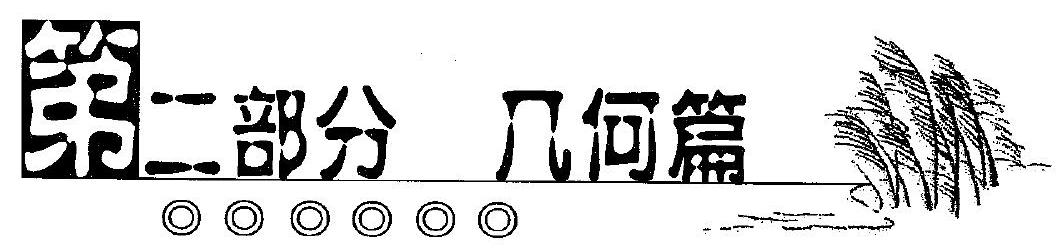
\includegraphics[max width=\textwidth, center]{2024_10_30_21385cc68d0979b6f3f8g-043}

平面几何是一个直老的数学分支,它不仅研究图形之间的位置关系与度量关系,也涉及平移、旋转、翻折等几何变换的动态属性.学习平面几何的过程,不仅能加强逻辑的严密性,也能利用代数技巧和数论中的某些知誤,做到数与形的有机结合. 在本章,我们从几个角度来重现几何中的一些基本观点。

业务:初高中联赛班、培优班、美国高中数学、教师培训、机构教学产品研发、讲义资料出售等

利用图形的面积公式,可以解决许多与面积相关的问题。对于常见的特殊图形面积的计算,一般直接使用公式或等积变换,对于非常规图形面积的计算,可通过图形的割补,以及图形的运动(平移、旋转、翻折)来转换成特殊图形面积问题。有时题目中并没有直接涉及面积,但可以通过对同一图形面积的不同算法,推出需要的代数或几何关系,从而使问题获解。

例1 如图 2-1-1:长方形 $A B C D$ 的面积是 2012 平方厘米,梯形 $A E G F$ 的顶点 $F$ 在 $B C$上, $D$ 是腰 $E G$ 的中点,试求梯形 $A E G F$ 的面积。

【分析】重点关注矩形 $A B C D 、 \triangle D F A$ 和梯形 $A E G F$ 的面积关系。

【解】取 $A F$ 的中点 $K$ ,连结 $D K 、 D F$ 。\\
由题意, $D K$ 是梯形 $A E G F$ 的中位线,因此,\\
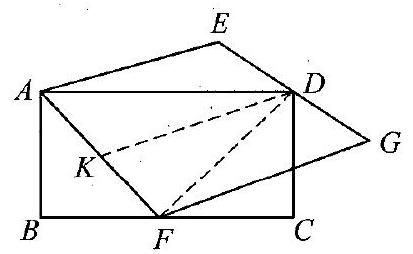
\includegraphics[max width=\textwidth, center]{2024_10_30_21385cc68d0979b6f3f8g-045(1)}

\section*{图 2-1-1}
\begin{align*}
D K / / A E / / F G, D K=\frac{1}{2}(A E+F G)
\end{align*}

所以\\
\begin{align*}
\frac{S_{\triangle A E D}}{S_{\triangle A K D}}=\frac{A E}{D K}, \frac{S_{\triangle D F G}}{S_{\triangle D F K}}=\frac{F G}{D K}
\end{align*}

由 $K$ 为 $A F$ 中点, 知\\
\begin{align*}
S_{\triangle A D K}=S_{\triangle F D K}, S_{\triangle A E D}+S_{\triangle D F G}=S_{\triangle A F D},
\end{align*}\\
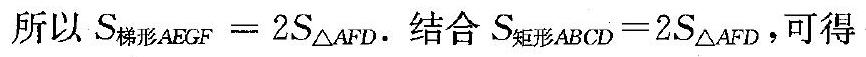
\includegraphics[max width=\textwidth, center]{2024_10_30_21385cc68d0979b6f3f8g-045}\\
\begin{align*}
S_{\text {槏形AEGF }}=S_{\text {矩形 } A B C D}=2012 .
\end{align*}

【注】 通过本题可了解几种常见的面积变换. 也可延长 $A E$ 和 $F D$ 交于一点,通过全等方法证明 $S_{\text {粎形AEGF }}=2 S_{\triangle A D F}$ 。

例2 如图 2-1-2:在梯形 $A B C D$ 中, $A D / / B C, A D: B C=1: 2, F$ 为线段 $A B$ 上的点, $E$ 为线段 $F C$ 上的点,且 $S_{\triangle A O F}: S_{\triangle D O E}=1: 3, S_{\triangle B E F}=24$ ,求 $\triangle A O F$ 的面积。

【分析】由于平行线间的距离处处相等,可将其作为一些三角形的高之和,进行面积的变换。

【解】过点 $E$ 作 $A D$ 的垂线,分别交 $A D$ 、 $B C$ 于点 $N 、 M$ 。过点 $F$ 作 $A D$ 的垂线,分别交 $D A$ 延长线及 $B C$ 于点 $Q 、 P$ 。\\
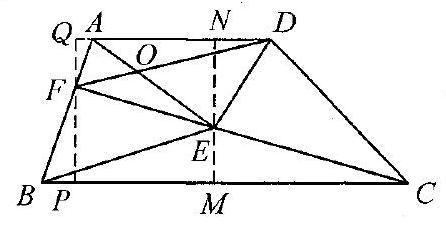
\includegraphics[max width=\textwidth, center]{2024_10_30_21385cc68d0979b6f3f8g-046}

图2-1-2

由于 $A D / / B C$ ,故 $P Q=M N$ 。\\
所以, $Q F+F P=N E+E M$ ,即 $F P-E M=N E-Q F$ 。从而\\
\begin{align*}
\begin{aligned}
S_{\triangle A E D}-S_{\triangle A F D} & =\frac{1}{2}(E N-F Q) \cdot A D \\
& =\frac{1}{2}(P F-M E) \cdot \frac{1}{2} B C \\
& =\frac{1}{2}\left(S_{\triangle B F C}-S_{\triangle B E C}\right) \\
& =\frac{1}{2} S_{\triangle B F E}=12
\end{aligned}
\end{align*}

由 $S_{\triangle A O F}: S_{\triangle D O E}=1: 3$, 知\\
\begin{align*}
S_{\triangle A E D}-S_{\triangle A F D}=S_{\triangle D O E}-S_{\triangle A O F}=2 S_{\triangle A O F}=12
\end{align*}

所以 $S_{\triangle A O F}=6$.\\
【注】本题虽然只用了最基本的面积公式 $S=\frac{1}{2} a h$ ,但发现了三角形高的差不变的性质,巧妙地转换成面积的差的关系。在解题中要善于发现题中隐藏的不变量。

例3 如图 2-1-3: $P$ 是 $\triangle A B C$ 内的一点, 连结 $A P 、 B P 、 C P$ 并延长,分别与 $B C 、 A C 、 A B$ 交于点 $D$ 、 $E 、 F$. 已知 $A P=6, B P=9, D P=6, E P=3, C F=20$ 。求 $\triangle A B C$ 的面积

【分析】可围绕 $P$ 为 $A D$ 中点这个条件构造平行线,求出其余未知线段的长度。再利用海伦公式及面积关系求解。

【解】 过点 $D$ 作 $A E$ 的平行线交 $B P$ 于点 $M$, 过点 $D$ 作 $A B$ 的平行线交 $C P$ 于点 $N$.

因为 $A P=P D=6$ 且 $D M / / A E$, 得\\
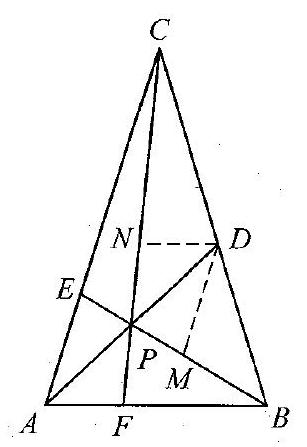
\includegraphics[max width=\textwidth, center]{2024_10_30_21385cc68d0979b6f3f8g-046(1)}

图 2-1-3\\
\begin{align*}
E P=M P=3,
\end{align*}

进而, $E M=6, B M=6$ ,即 $M$ 为 $B E$ 的中点,所以 $D$ 为 $B C$ 的中点,即 $C D=B D$ 。\\
因为 $D N / / A B$, 所以 $N$ 为 $C F$ 的中点, $P$ 为 $N F$ 的中点。\\
从而 $C N=F N=10, N P=P F=5, C P=15$ 。\\
由中线长公式: $P D^{2}=\frac{1}{2} C P^{2}+\frac{1}{2} B P^{2}-\frac{1}{4} B C^{2}$ 可得, $B C=6 \sqrt{13}$, $C D=3 \sqrt{13}$.

由海伦公式: $S_{\triangle C P D}=27$ ,故 $S_{\triangle A B C}=4 S_{\triangle C P D}=108$.\\
【注】常见的三角形面积公式有:\\
\begin{align*}
\begin{aligned}
S_{\triangle A B C} & =\frac{1}{2} a h_{a}=\frac{1}{2} b h_{b}=\frac{1}{2} c h_{c} \\
& =\frac{1}{2} a b \sin C=\frac{1}{2} b c \sin A=\frac{1}{2} a c \sin B \\
& =\frac{a b c}{4 R} \\
& =2 R^{2} \sin A \sin B \sin C \\
& =p r \\
& =\sqrt{p(p-a)(p-b)(p-c)} .
\end{aligned}
\end{align*}

其中 $\triangle A B C$ 三边为 $a 、 b 、 c$ ,对应边上的高为 $h_{a} 、 h_{b} 、 h_{c}$ ,外接圆、内切圆半径分别为 $R 、 r$, 半周长 $p=\frac{1}{2}(a+b+c)$.

例4 如图 2-1-4:设凸四边形 $A B C D$ 内接于以 $O$ 为中心的圆,且两条对角线相互垂直. 求证:折线 $A O C$ 分该四边形面积相等的两部分。

【分析】对角线互相垂直的四边形面积等于对角线乘积的一半。

【证明】过点 $O$ 作 $O P \perp B D$ ,垂足为点 $P$ 。\\
故 $S_{\text {四边形 } A O C D}=S_{\triangle A O C}+S_{\triangle A C D}=\frac{1}{2} A C \cdot P D$ 。\\
因为 $O P \perp B D$ ,故 $P D=\frac{1}{2} B D$ ,所以\\
\begin{align*}
S_{\text {四边形 } A O C D}=\frac{1}{4} A C \cdot B D .
\end{align*}\\
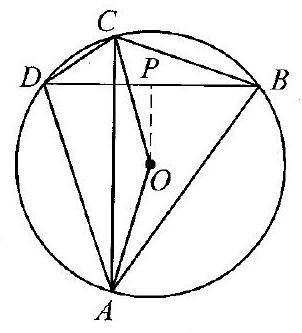
\includegraphics[max width=\textwidth, center]{2024_10_30_21385cc68d0979b6f3f8g-047}

图 2-1-4

因为 $A C \perp B D$, 所以 $S_{\text {四边形 } A B C D}=\frac{1}{2} A C \cdot B D$ 。\\
所以 $S_{\text {四边形 } A B C D}=2 S_{\text {四边形 } A O C D}$, 即折线 $A O C$ 分该四边形面积相等的两部分.

例5 设 $P$ 是 $\triangle A B C$ 内一点, 延长 $A P 、 B P 、 C P$ 与对边相交于点 $D 、 E$ 、 $F$ 。设 $A P=a, B P=b, C P=c$ ,且 $a+b+c=43$ , $P D=P E=P F=d=3$ ,求 $a b c$ 的值。

【分析】可将条件中相应线段比转换成面积比,通过面积相等的关系人手解题。

【解】由共边比例定理可得: $\frac{S_{\triangle P A B}}{S_{\triangle A B C}}=\frac{d}{c+d}$.\\
同理: $\frac{S_{\triangle P B C}}{S_{\triangle A B C}}=\frac{d}{a+d}, \frac{S_{\triangle P C A}}{S_{\triangle A B C}}=\frac{d}{b+d}$.\\
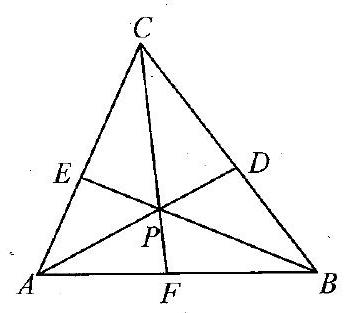
\includegraphics[max width=\textwidth, center]{2024_10_30_21385cc68d0979b6f3f8g-048(1)}

图2-1-5

故 $\frac{d}{a+d}+\frac{d}{b+d}+\frac{d}{c+d}=\frac{S_{\triangle P A B}+S_{\triangle P B C}+S_{\triangle P C A}}{S_{\triangle A B C}}=\frac{S_{\triangle A B C}}{S_{\triangle A B C}}=1$.\\
从而 $2 d^{3}+(a+b+c) d^{2}-a b c=0$ ,所以 $a b c=441$ 。\\
例 6 如图 2-1-6:设 $\triangle A B C$ 的三条中线 $A D 、 B E 、 C F$ 交于点 $G$ ,且 $\triangle A G F, \triangle C G D$ 和 $\triangle B G D$ 的内切圆半径都相同。证明: $\triangle A B C$ 是正三角形。

【分析】利用 $S=p \cdot r$ ,及面积和内切圆半径相等的条件,得到相应的边的关系,再进行论证。

【证明】设 $\triangle A F G$ 和 $\triangle C D G$ 的内心分别为 $I_{1}$和 $I_{2}$ ,过 $I_{1}$ 作 $I_{1} M_{1} \perp F G$ 于点 $M_{1}$ ,过 $I_{2}$ 作 $I_{2} M_{2} \perp$ $G D$ 于点 $M_{2}$ ,连结 $I_{1} G$ 和 $I_{2} G$ 。

因为 $D$ 为 $B C$ 的中点,所以 $B D=C D$ ,从而 $S_{\triangle B D G}=S_{\triangle C D G}$. 故\\
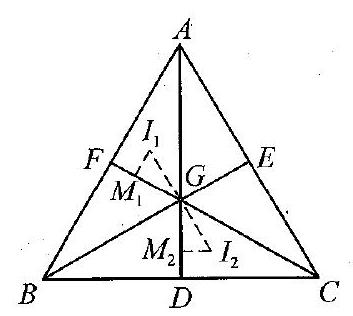
\includegraphics[max width=\textwidth, center]{2024_10_30_21385cc68d0979b6f3f8g-048}

图2-1-6\\
$\frac{1}{2}(B D+D G+B G) \cdot r=\frac{1}{2}(C D+D G+G C) \cdot r$.

故 $B G=C G, G D \perp B C$ 。\\
进而 $A D$ 垂直平分 $B C$ ,所以 $A B=A C$ 。\\
在 Rt $\triangle I_{1} M_{1} G$ 和 Rt $\triangle I_{2} M_{2} G$ 中有: $I_{1} M_{1}=I_{2} M_{2}$ ,且有\\
\begin{align*}
\angle I_{1} G M_{1}=\frac{1}{2} \angle A G F=\frac{1}{2} \angle D G C=\angle I_{2} G M_{2}
\end{align*}

从而 $\mathrm{Rt} \triangle I_{1} M_{1} G \cong \mathrm{Rt} \triangle I_{2} M_{2} G$ ,所以 $G M_{1}=G M_{2}$ 。\\
因为\\
\begin{align*}
G M_{1}=\frac{1}{2}(A G+G F-A F), G M_{2}=\frac{1}{2}(G D+G C-C D)
\end{align*}

故 $A G+G F-A F=G D+G C-C D$ 。\\
因为 $A F+F G+G A=G D+D C+C G$ ,所以 $A F=C D$ 。\\
因而 $A B=B C$ 。所以 $A B=A C=B C$ ,即 $\triangle A B C$ 为正三角形。\\
【注】利用三角形面积的不同表达式,可以建立各种等量关系,帮助我

们从中发现规律,得到解题思路。\\
例7 如图 2-1-7: $\triangle A B C$ 的三边上 $B C=a, C A=b, A B=c, a, b$ , $c$ 都是整数,且 $a, b$ 的最大公约数为 2 。点 $G$ 和点 $I$ 分别为 $\triangle A B C$ 的重心和内心,且 $\angle G I C=90^{\circ}$ 。求 $\triangle A B C$ 的周长。

【分析】过 $G I$ 的直线截得等腰 $\triangle P Q C$ ,利用重心和内心的性质将 $\triangle P Q C$ 的面积算两次,再进行分析。

【解】过 $G I$ 的直线与边 $B C 、 C A$ 分别交于点 $P 、 Q$ 。过 $G$ 作 $G E \perp B C, G F \perp A C$ ,垂足分别为 $E 、 F$ ,连结 $G C$ 。

设 $\triangle A B C$ 的内切圆的半径为 $r, B C 、 C A$ 边\\
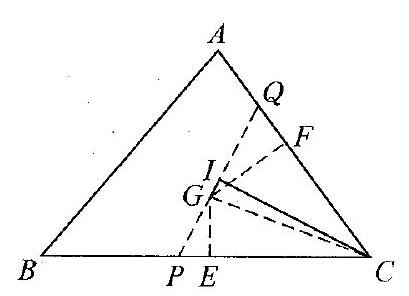
\includegraphics[max width=\textwidth, center]{2024_10_30_21385cc68d0979b6f3f8g-049}

图2-1-7

上的高的长分别为 $h_{a}, h_{b}$ 。

因为 $I$ 为 $\triangle A B C$ 的内心,所以 $\angle P C I=\angle Q C I$ 。\\
由题意: $\angle Q I C=\angle P I C=90^{\circ}$ ,故 $\triangle P I C \cong \triangle Q I C$ ,所以 $P C=Q C$ 。\\
一方面: $\quad S_{\triangle P Q C}=S_{\triangle P I C}+S_{\triangle Q I C}=\frac{1}{2} \cdot P C \cdot r+\frac{1}{2} \cdot Q C \cdot r$ ,\\
另一方面: $\quad S_{\triangle P Q C}=S_{\triangle G P C}+S_{\triangle G Q C}=\frac{1}{2} \cdot P C \cdot(G E+G F)$ ,\\
故 $2 r=G E+G F=\frac{1}{3}\left(h_{a}+h_{b}\right)$.\\
故 $\frac{4 S_{\triangle A B C}}{a+b+c}=\frac{1}{3} \cdot\left(\frac{2 S_{\triangle A B C}}{a}+\frac{2 S_{\triangle A B C}}{b}\right)$, 所以 $a+b+c=\frac{6 a b}{a+b}$.\\
因为 $\triangle A B C$ 的重心 $G$ 和内心 $I$ 不重合,故 $\triangle A B C$ 不是正三角形。\\
若 $a=b$ ,则 $a=b=2, c=2$ ,矛盾!\\
从而 $a \neq b$, 不妨设 $a>b, a=2 a_{1}, b=2 b_{1},\left(a_{1}, b_{1}\right)=1$. 由 $\frac{6 a b}{a+b}=$ $\frac{12 a_{1} b_{1}}{a_{1}+b_{1}}$ 为整数知, $a_{1}+b_{1} \mid 12$ ,即 $a+b \mid 24$ 。因此 $a+b=6,8,12,24$.

经检验,只有当 $a=14, b=10, c=11$ 时满足条件,故 $a+b+c=35$ ,即 $\triangle A B C$ 的周长为 35 。

【注】本题虽然没有直接涉及面积,但借助于图形面积知识解答,往往事半功倍。

\section{练 32.1}
䨩 如图:已知正方形 $A B C D$ 的面积为 35 平方厘米, $E 、 F$ 分别为边 $A B 、 B C$

上的点, $A F$ 与 $C E$ 相交于点 $G$ ,并且 $\triangle A B F$ 的面积为 5 平方厘米, $\triangle B C E$ 的面积为 14 平方厘米。求四边形 $B E G F$ 的面积。\\
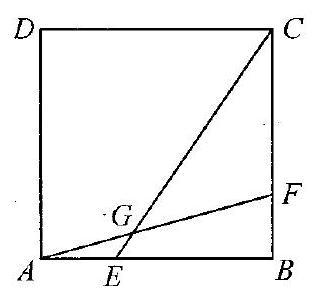
\includegraphics[max width=\textwidth, center]{2024_10_30_21385cc68d0979b6f3f8g-050}\\
(第1题)\\
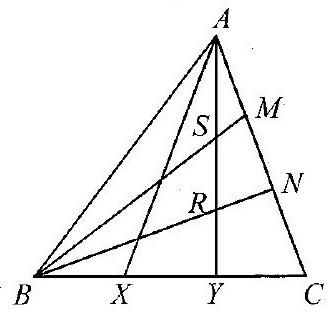
\includegraphics[max width=\textwidth, center]{2024_10_30_21385cc68d0979b6f3f8g-050(3)}\\
(第2题)

2 如图:点 $M$ 和 $N$ 三等分 $A C$ ,点 $X$ 和 $Y$ 三等分 $B C, A Y$ 与 $B M 、 B N$ 分别交于点 $S 、 R$ 。求四边形 $S R N M$ 的面积与 $\triangle A B C$ 的面积之比。\\
设 $\triangle A B C$ 三边上的三个内接正方形(有两个顶点在三角形的一边上,另两个顶点分别在三角形另两边上)的面积都相等。证明: $\triangle A B C$ 为正三角形。\\
4 如图:过 $\triangle A B C$ 内部一点 $P$ ,作三条分别与三边平行的直线,所得的三个三角形 $t_{1}, t_{2}, t_{3}$ 的面积分别为 $4,9,49$ 。求 $S_{\triangle A B C}$ 的值。\\
5 是否存在三个顶点均为格点的正三角形?\\
6. 已知四边形 $A B C D$ 的面积为 $32, A B 、 C D 、 A C$的长都是整数,且它们的和为 16 。\\
(1)这样的四边形有几个?\\
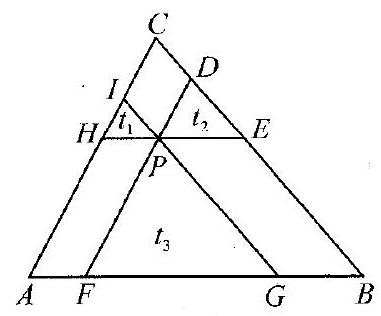
\includegraphics[max width=\textwidth, center]{2024_10_30_21385cc68d0979b6f3f8g-050(2)}\\
(第4题)\\
(2)求这样的四边形边长的平方和的最小值。\\
知 $\triangle A B C$ 的三边长恰是三个连续正整数,其周长和面积分别为 $p_{1}$ 和 $S_{1}$ 。将 $\triangle A B C$ 的三边都增加 10 ,所得到的新 $\triangle A^{\prime} B^{\prime} C^{\prime}$ 的周长和面积分别为 $p_{2}$ 和 $S_{2}$ 。当 $p_{1} p_{2}=S_{1} S_{2}$ 时,求 $\triangle A B C$ 的三边长。\\
8 设 $I$ 是 $\triangle A B C$ 内心, $I$ 在 $A B 、 B C 、 C A$ 上的射影分别是 $L 、 M 、 N, M I$延长后,交 $L N$ 于点 $T, A T$ 延长后与 $B C$ 交于点 $Q$ 。求证: $B Q=C Q$ 。\\
量在 Rt $\triangle A B C$ 中, $\angle A=90^{\circ}, \angle B$ 和 $\angle C$ 的内角平分线交于点 $I$ ,分别交对边于 $D$ 和 $E$ 两点。证明:四边形 $B C D E$ 的面积是 $\triangle B I C$ 面积的两倍。\\
10 如图:在锐角 $\triangle A B C$ 的 $B C$ 边上有两点 $E 、 F$ ,满足 $\angle B A E=\angle C A F$ ,作 $F M \perp A B, F N \perp A C, M$ 、 $N$ 是垂足,延长 $A E$ 交 $\triangle A B C$ 的外接圆于点 $D$ 。证明:四边形 $A M D N$ 与 $\triangle A B C$ 的面积相等。\\
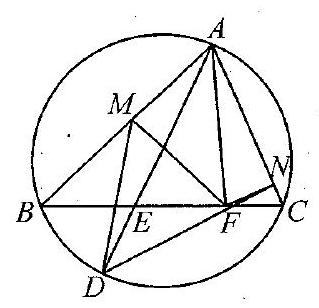
\includegraphics[max width=\textwidth, center]{2024_10_30_21385cc68d0979b6f3f8g-050(1)}\\
(第 10 题)

与代数变换的重要性一样,几何变换同样在几何问题的解决中也起着非常重要的作用。通过几何变换,可以把分散的线段、角相对集中起来,从而使已知条件集中在一个我们所熟知的基本图形之中,然后利用新的图形的性质对原图形进行研究,从而使问题得以转化。

例1 如图 2-2-1:设 $I$ 是 $\triangle A B C$ 的垂心。 求证: $A I^{2}+B C^{2}=B I^{2}+A C^{2}=C I^{2}+A B^{2}$ 。

【分析】对于 $\triangle A B C$ 各边来说,结论是轮换式,于是只需证得某一个等式即可。显然等式每边都是两线段的平方和,故可考虑构造相应的直角三角形。

【证明】 分别过点 $B 、 I$ 作 $A I 、 A B$ 的平行线,两线交于 $P$ 点,连结 $P C$ 。\\
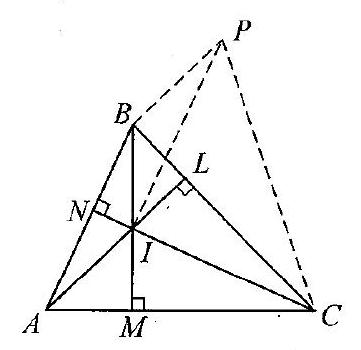
\includegraphics[max width=\textwidth, center]{2024_10_30_21385cc68d0979b6f3f8g-051(1)}

图2-2-1

由条件可知:四边形 $A I P B$ 为平行四边形,从而 $B P=A I, \angle P B C=\angle A L B=90^{\circ}$ ,所以\\
\begin{align*}
P C^{2}=P B^{2}+B C^{2}=A I^{2}+B C^{2} ;
\end{align*}

同理: $P I=A B, \angle P I C=\angle B N C=90^{\circ}$ 。\\
故 $P C^{2}=C I^{2}+P I^{2}=C I^{2}+A B^{2}$ ,所以 $A I^{2}+B C^{2}=C I^{2}+A B^{2}$ ;\\
同理: $A I^{2}+B C^{2}=B I^{2}+A C^{2}$ 。\\
所以 $A I^{2}+B C^{2}=B I^{2}+A C^{2}=C I^{2}+A B^{2}$ 。\\
例 2 已知 $\triangle A B C$ 的三条中线的长为 $3 、 4 、 5$. 求 $\triangle A B C$ 的面积.\\
【分析】 设 $\triangle A B C$ 的中线 $A D=3$ , $B E=4, C F=5$ 。现考虑通过平移使三条中线集中在一起,构成一个确定的三角形,再分析面积间的数量关系。

【解法一】过 $F$ 作 $F K \underline{I} E C$ ,连结 $K A 、$ $K E 、 K B 、 E F$ 。\\
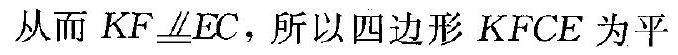
\includegraphics[max width=\textwidth, center]{2024_10_30_21385cc68d0979b6f3f8g-051(2)}\\
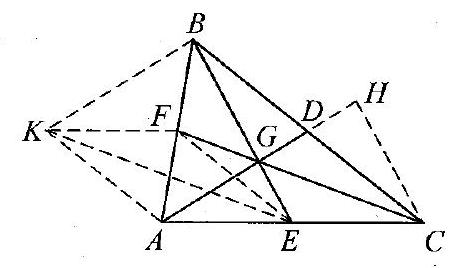
\includegraphics[max width=\textwidth, center]{2024_10_30_21385cc68d0979b6f3f8g-051}

图2-2-2

行四边形,进而 $K F=E C$ 。\\
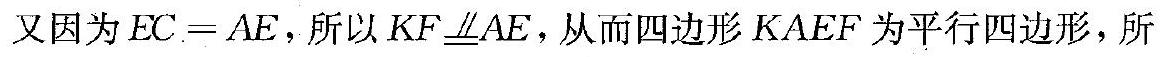
\includegraphics[max width=\textwidth]{2024_10_30_21385cc68d0979b6f3f8g-052}以 $K A \underline{ }$

因为 $E F \cong \frac{1}{2} B C, B D=\frac{1}{2} B C$ ,故 $A K \Perp B D$ 。\\
因此四边形 $B K A D$ 为平行四边形。从而 $B K=A D$ 。\\
所以 $\triangle B K E$ 是以 $\triangle A B C$ 三边中线长为边长的三角形。\\
因为 $5^{2}=3^{2}+4^{2}$, 所以 $\triangle B K E$ 为直角三角形, $S_{\triangle B K E}=6$ 。\\
因为 $S_{\triangle B F K}=\frac{1}{4} S_{A D B K}=\frac{1}{4} S_{\triangle A B C}, S_{\triangle B E F}=\frac{1}{4} S_{\triangle A B C}, S_{\triangle E F K}=S_{\triangle A E F}=$ $\frac{1}{4} S_{\triangle A B C}$.

从而 $S_{\triangle B K E}=\frac{3}{4} S_{\triangle A B C}, S_{\triangle A B C}=8$.\\
【注】可将问题一般化,设 $\triangle A B C$ 三边上中线的长度分别为 $m_{a}, m_{b}$ , $m_{c}$ ,则有:\\
\begin{align*}
S_{\triangle A B C}=\frac{4}{3} \sqrt{p\left(p-m_{a}\right)\left(p-m_{b}\right)\left(p-m_{c}\right)}
\end{align*}

其中 $p=\frac{1}{2}\left(m_{a}+m_{b}+m_{c}\right)$.\\
【解法二】利用重心的性质,构造出三角形,结合以 $A D 、 B E 、 C F$ 长为边的三角形与其相似,再求解面积。

延长 $G D$ 至点 $H$ ,使 $G D=H D$ ,连结 $H C$ 。\\
易证: $\triangle B D G \cong \triangle C D H$ ,故 $B G=C H=\frac{2}{3} B E$ 。\\
因为 $C G=\frac{2}{3} C F, G H=2 G D=\frac{2}{3} A D$ ,故 $C G^{2}=H G^{2}+H C^{2}$ ,因此 $S_{\triangle G H C}=\left(\frac{2}{3}\right)^{2} \times 6=\frac{8}{3}$, 所以 $S_{\triangle C D G}=\frac{4}{3}$.

又因为 $G$ 为 $\triangle A B C$ 的重心,所以 $S_{\triangle A B C}=8$ 。\\
【注】由以上两个例题可知,图形经过适当的平移可以使已知条件和结论中的图形元素得以延伸,再通过某些桥梁得以联系和统一。

例3 如图 2-2-3:在 $\triangle A B C$ 外作等腰 Rt $\triangle A B D$ 和等腰 Rt $\triangle A C E$ ,且 $\angle B A D=\angle C A E=90^{\circ}, A M$ 为 $\triangle A B C$ 中 $B C$ 边上的中线, 连结 $D E$ 。求证: $D E=2 A M$.

【分析】由 $M$ 为 $B C$ 中点, 可利用中线加倍得到 $A F=2 A M$, 再证 $A F=$\\
$D E$. 注意到 $\triangle B M F$ 可通过 $\triangle C M A$ 旋转得到,故可利用图形旋转相关性质思考。

【证明】延长 $A M$ 至 $F$ ,使 $A M=F M$ ,连结 $B F$ 。\\
因为 $B M=C M, A M=F M, \angle A M C=\angle F M B$ ,所以 $\triangle A M C \cong \triangle F M B$ 。

从而 $\angle F=\angle M A C, B F=A C$ ,所以\\
\begin{align*}
\begin{aligned}
\angle A B F & =180^{\circ}-\angle B A F-\angle F \\
& =180^{\circ}-\angle B A F-\angle M A C \\
& =180^{\circ}-\left(180^{\circ}-\angle D A E\right)=\angle D A E
\end{aligned}
\end{align*}\\
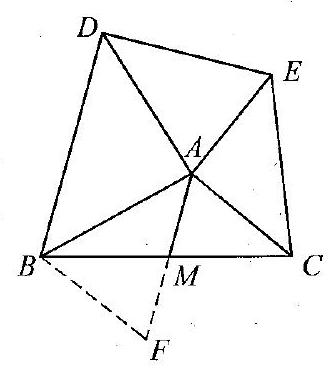
\includegraphics[max width=\textwidth, center]{2024_10_30_21385cc68d0979b6f3f8g-053}

图2-2-3

又因为 $A D=A B, A E=A C$, 故 $A E=B F$.\\
因而 $\triangle A D E \cong \triangle B A F, D E=A F=2 A M$ 。\\
【注】图形的旋转可通过构造全等来实现,旋转变换即全等变换的一种,在几何证明题中,常常以图形旋转的观点来研究,是常用策略。

例4 如图 2-2-4:正方形 $A B C D$ 内一点 $E, E$ 到 $A 、 B 、 C$ 三点的距离之和的最小值为 $\sqrt{2}+\sqrt{6}$ ,求此正方形的边长。

【分析】利用图形的旋转,将三条线段转换为首尾顺次连接,再利用两点间线段最短求最值问题。

【解】 将 $\triangle A B E$ 绕 $A$ 点顺时针旋转 $60^{\circ}$ 到 $\triangle A M N$ ,连结 $N E, M B$ 。过 $M$ 作 $M P \perp B C$ ,垂足为 $P$ 。\\
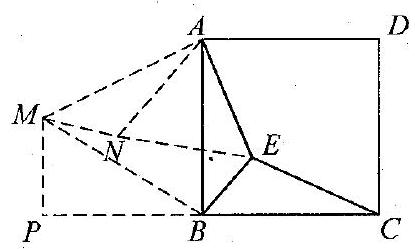
\includegraphics[max width=\textwidth, center]{2024_10_30_21385cc68d0979b6f3f8g-053(1)}

图2-2-4

由题意: $A E=A N, \angle N A E=60^{\circ}$ ,从而 $\triangle A N E$ 为等边三角形. 故 $A E=N E$ ,所以\\
\begin{align*}
A E+B E+C E=M N+N E+E C
\end{align*}

当 $A E+B E+C E$ 最小时,折线 $M N E C$ 为线段,且 $M C=\sqrt{2}+\sqrt{6}$ ;\\
同理: $\triangle A M B$ 为等边三角形。\\
所以 $A B=B C=B M, \angle M B A=60^{\circ}$.\\
设 $A B=x$, 则 $P M=\frac{1}{2} x, P B=\frac{\sqrt{3}}{2} x$, 在 Rt $\triangle M P C$ 中:\\
\begin{align*}
(\sqrt{2}+\sqrt{6})^{2}=\left(\frac{1}{2} x\right)^{2}+\left(\frac{\sqrt{3}}{2} x+x\right)^{2}
\end{align*}

解得: $x=2$, 即 $A B=2$, 正方形边长为 2 .

例5 如图 2-2-5:在正 $\triangle A B C$ 内有一点 $P, P$ 到三个顶点 $A 、 B 、 C$ 的距离分别为 $a 、 b 、 c$, 求 $\triangle A B C$ 的面积。

【分析】由于 $A P 、 B P 、 C P$ 为已知,故可将 $A P 、 B P 、 C P$ 移至一个三角形。为此可分别旋转 $\triangle A B P 、 \triangle B P C 、 \triangle P C A$ ,通过求六边形 $A F B D C E$的面积求解 $\triangle A B C$ 的面积。

【解】分别将 $\triangle A B P 、 \triangle B C P 、 \triangle C A P$ 绕着 $B$ 、 $C 、 A$ 顺时针旋转 $60^{\circ}$ ,得到 $\triangle C B D 、 \triangle A C E$ 、 $\triangle B A F$ 。连结 $P D 、 P E 、 P F$ 。\\
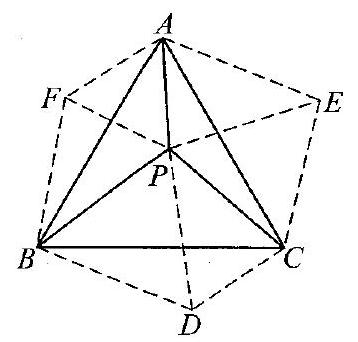
\includegraphics[max width=\textwidth, center]{2024_10_30_21385cc68d0979b6f3f8g-054}

图2-2-5

故 $S_{\text {六边形 } A F B D C E}=2 S_{\triangle A B C}$.\\
因为 $A P=A F, \angle P A F=60^{\circ}$ ,所以 $\triangle A P F$ 为等边三角形,边长为 $a$ 。从而 $P F=A P$ 。

因为 $B F=P C$ ,故 $\triangle B P F$ 的三边长分别为 $a, b, c$ ;\\
同理: $\triangle B P D$ 是边长为 $b$ 的等边三角形, $\triangle C P E$ 是边长为 $c$ 的等边三角形,

由于 $\triangle D P C$ 和 $\triangle E P A$ 的三边长都分别为 $a, b, c$.\\
因此 $S_{\text {六边形 } A F B D C E}=\frac{\sqrt{3}}{4}\left(a^{2}+b^{2}+c^{2}\right)+3 \sqrt{p(p-a)(p-b)(p-c)}$.\\
所以 $S_{\triangle A B C}=\frac{\sqrt{3}}{8}\left(a^{2}+b^{2}+c^{2}\right)+\frac{3}{2} \sqrt{p(p-a)(p-b)(p-c)}$, 其中 $p=\frac{1}{2}(a+b+c)$.

【注】利用图形的旋转可构造等边三角形或等腰直角三角形,实现线段和角度的转换,使原来分散的线段和角集中起来或有序地排列起来,得到新的图形以方便研究。

例6 如图 2-2-6: 在 $\triangle A B C$ 中, $A D$ 是角平分线, $B E=C F$, 点 $M 、 N$分别是 $B C$ 和 $E F$ 的中点。求证: $M N / / A D$ 。

【分析】利用等腰三角形轴对称性构造中点,再结合条件中的中点,构造平行四边形来论证平行关系。

【证明】过 $E$ 作 $A D$ 的垂线,交 $A D$ 于点 $G$ ,交 $A C$ 于点 $S$ 。过 $B$ 作 $A D$ 的垂线, 交 $A D$ 于点 $H$, 交 $A C$ 于点 $T$ 。连结 $G N, H M$ 。

因为 $A D$ 平分 $\angle B A C$ ,所以 $\angle E A G=\angle S A G$ 。\\
因为 $A D \perp E S$ ,故 $\angle A G E=\angle A G S=90^{\circ}$ 。\\
所以 $\triangle A E G \cong \triangle A S G$ 。\\
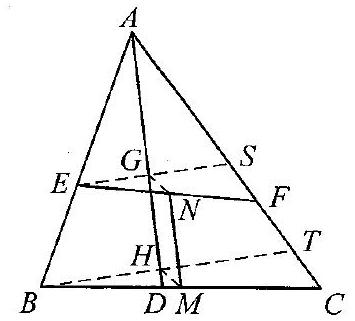
\includegraphics[max width=\textwidth, center]{2024_10_30_21385cc68d0979b6f3f8g-054(1)}

图2-2-6

故 $A E=A S, E G=S G$ 。\\
同理: $A B=A T, B H=T H$.\\
又因为 $N$ 为 $E F$ 的中点,故 $G N \Perp \frac{1}{2} S F$ ;同理: $M H \Perp \frac{1}{2} C T$ 。\\
因为 $B E=F C$ ,所以 $S T=F C$ ,从而 $S F=C T$ ,进而 $G N \Perp H M$ 。\\
故四边形 $G N M H$ 为平行四边形,所以 $M N / / A D$ 。\\
【注】本题是把角平分线作为翻折轴来进行解题的。用角平分线作为翻折轴,可以使翻折图形落至原来图形的另一侧,而且对应点的连线被角平分线垂直平分. 这样不仅可以增加图形的直观性,而且增强条件与结论间的逻辑联系。

例 7 如图 2-2-7:在矩形 $A B C D$ 中, $A B=20, B C=10$ ,若在 $A B$ 、 $A C$ 上各取一点 $N 、 M$, 使得 $B M+M N$ 的值最小, 求这个最小值.

【分析】作 $B$ 关于 $A C$ 的对称点 $E$ ,即求折线 $E M N$ 的最小值,这个最小值为点 $E$ 到 $A B$ 垂线段的距离。

【解】作 $B$ 关于直线 $A C$ 的对称点 $E$, 连结 $A E$ 、 $B E 、 M E$ 。过点 $E$ 作 $A B$ 的垂线, 交 $A B 、 A C$ 于点 $F 、 G$.

由 $B M+M N=E M+M N \geqslant E F$ ,所以 $B M+$\\
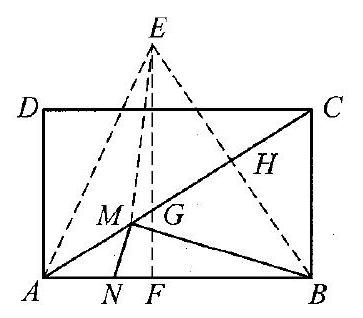
\includegraphics[max width=\textwidth, center]{2024_10_30_21385cc68d0979b6f3f8g-055}

图2-2-7\\
$M N$ 的最小值为 $E F$ 。

因为 $2 S_{\triangle A B C}=A B \cdot B C=A C \cdot B H$, 故 $B H=4 \sqrt{5}, B E=2 B H=8 \sqrt{5}$ 。\\
所以 $A H=\sqrt{A B^{2}-B H^{2}}=8 \sqrt{5}$ 。\\
因为 $2 S_{\triangle A B E}=A B \cdot E F=B E \cdot A H$ ,故 $E F=16$ 。\\
所以 $B M+M N$ 的最小值为 16 ,此时 $N$ 和 $F$ 重合, $M$ 和 $G$ 重合。\\
例8 如图 2-2-8:在 $\triangle A B C$ 中, $\angle A B C=90^{\circ}, A B=B C, P$ 为三角形内一点,分别作 $P$ 关于 $B C 、 C A 、 A B$ 的对称点 $A^{\prime} 、 B^{\prime} 、 C^{\prime}$ 。若所得 $\triangle A^{\prime} B^{\prime} C^{\prime}$ 中, $\angle B^{\prime} A^{\prime} C^{\prime}=90^{\circ}, A^{\prime} B^{\prime}=A^{\prime} C^{\prime}$ 。求: $S_{\triangle A^{\prime} B^{\prime} C^{\prime}}: S_{\triangle A B C}$ 的值。

【分析】由对称性可得的五边形面积是 $\triangle A B C$面积的两倍,并且 $A C^{\prime} A^{\prime} B^{\prime}$ 是正方形。 $\triangle A^{\prime} B^{\prime} C$ 为等腰直角三角形。

【解】 连结 $P A 、 P B 、 P C 、 A C^{\prime} 、 A B^{\prime} 、 B A^{\prime}$ 、 $B C^{\prime} 、 C A^{\prime} 、 C B^{\prime}$ 。

由轴对称性知: $A C^{\prime}=A P=A B^{\prime}$ 。\\
$\angle C^{\prime} A B=\angle P A B, \angle B^{\prime} A C=\angle P A C$.\\
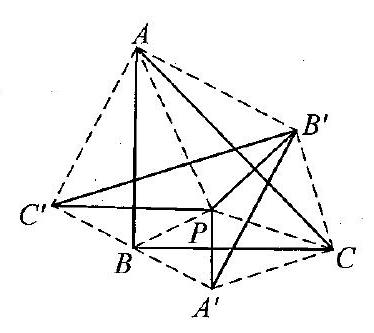
\includegraphics[max width=\textwidth, center]{2024_10_30_21385cc68d0979b6f3f8g-055(1)}

图2-2-8

因为 $\angle A B C=90^{\circ}, A B=B C$, 所以 $\angle B A C=45^{\circ}$. 故 $\angle B^{\prime} A C^{\prime}=90^{\circ}$;同理: $\angle A^{\prime} C B^{\prime}=90^{\circ}, \angle A^{\prime} B C^{\prime}=180^{\circ}$, 故 $C^{\prime} 、 B 、 A^{\prime}$ 三点共线.所以 $\triangle A B^{\prime} C^{\prime}$ 是等腰直角三角形。\\
因为 $\triangle A^{\prime} B^{\prime} C^{\prime}$ 也是等腰直角三角形,所以四边形 $A C^{\prime} A^{\prime} B^{\prime}$ 为正方形;同理: $\triangle A^{\prime} B^{\prime} C$ 为等腰直角三角形。

设 $A^{\prime} B^{\prime}=a$, 故. $S_{A^{\prime} B^{\prime} A C^{\prime}}=a^{2}, S_{\triangle A^{\prime} B^{\prime} C}=\frac{1}{4} a^{2}$, 故 $S_{A^{\prime} C B^{\prime} A C^{\prime}}=\frac{5}{4} a^{2}$.由轴对称性质: $S_{A^{\prime} C B^{\prime} A C^{\prime}}=2 S_{\triangle A B C}$, 故 $S_{\triangle A B C}=\frac{5}{8} a^{2}$.\\
故 $S_{\triangle A^{\prime} B^{\prime} C^{\prime}}: S_{\triangle A B C}=\frac{1}{2} a^{2}: \frac{5}{8} a^{2}=4: 5$.

\section{练 2.2}
目证明:如果七条直线两两相交,那么所得的角中至少有一个角小于 $26^{\circ}$.\\
2 如图:在"风车三角形"中, $A A^{\prime}=B B^{\prime}=C C^{\prime}=2, \angle A O B^{\prime}=\angle B O C^{\prime}=$ $\angle C O A^{\prime}=60^{\circ}$. 求证: $S_{\triangle A O B^{\prime}}+S_{\triangle B O C^{\prime}}+S_{\triangle C O A^{\prime}}<\sqrt{3}$.\\
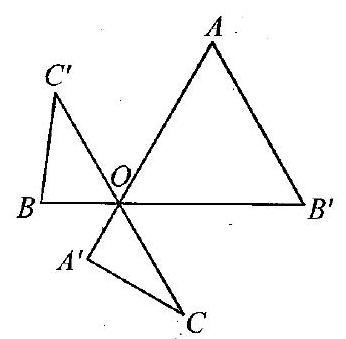
\includegraphics[max width=\textwidth, center]{2024_10_30_21385cc68d0979b6f3f8g-056}\\
(第2题)\\
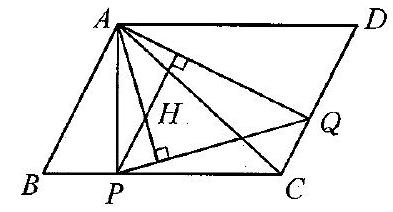
\includegraphics[max width=\textwidth, center]{2024_10_30_21385cc68d0979b6f3f8g-056(1)}\\
(第3题)\\
3. 如图: 在平行四边形 $A B C D$ 中, 由 $A$ 向另两边作垂线 $A P 、 A Q$, 已知 $P Q=a, A C=b, H$ 为 $\triangle A P Q$ 的垂心. 求 $A H$ 的值.\\
4 已知直角三角形 $A B C$ 中, 斜边 $A B$ 长为 $2, \angle A C B=90^{\circ}$, 三角形内一个动点到三个顶点的距离之和的最小值为 $\sqrt{7}$. 求这个直角三角形的两个锐角的大小。\\
国 如图: 在四边形 $A B C D$ 中, $\angle A B C=30^{\circ}, \angle A D C=60^{\circ}, A D=A C$. 证明: $B D^{2}=A B^{2}+B C^{2}$ 。\\
6 . 如图: 已知正方形 $A B C D$ 的边长为 $1, P 、 Q$ 是其内两点, 且 $\angle P A Q=$ $\angle P C Q=45^{\circ}$. 求 $S_{\triangle P A B}+S_{\triangle P C Q}+S_{\triangle Q A D}$ 的值.\\
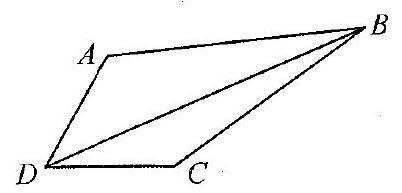
\includegraphics[max width=\textwidth, center]{2024_10_30_21385cc68d0979b6f3f8g-057}\\
(第 5 题)\\
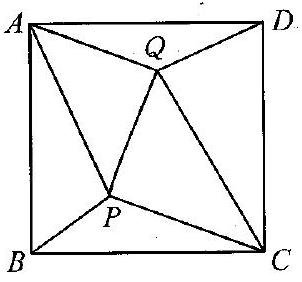
\includegraphics[max width=\textwidth, center]{2024_10_30_21385cc68d0979b6f3f8g-057(1)}\\
(第 6 题)

知点 $I$ 是锐角 $\triangle A B C$ 的内心, $A_{1} 、 B_{1} 、 C_{1}$ 分别是点 $I$ 关于边 $B C 、 C A$ 、 $A B$ 的对称点, 若点 $B$ 在 $\triangle A_{1} B_{1} C_{1}$ 的外接圆上, 求 $\angle A B C$ 的值.\\
8 已知在 $\triangle A B C$ 的边 $A B 、 A C$ 上分别取点 $Q 、 P$, 使得 $\angle P B C=\angle Q C B=$ $\frac{1}{2} \angle A$. 求证: $B Q=C P$ 。\\
9 已知 $\angle P O Q=30^{\circ}$, $A$ 为 $O Q$ 上一点, $B$ 为 $O P$ 上一点, 且 $O A=5$, $O B=12$. 在 $O B$ 上取点 $A_{1}$, 在 $A Q$ 上取点 $A_{2}$, 设 $l=A A_{1}+A A_{2}+A_{2} B$,求 $l$ 的最小值。\\
10 是否存在这样的 $\square A B C D$ ,使之具有如下两个性质:\\
(1)两条对角线 $A C$ 与 $B D$ 的长是互质的整数;\\
(2) 若分别以直线 $A C 、 B D$ 为对称轴作出 $\triangle A C D$ 和 $\triangle B C D$ 的对称 $\triangle A C D^{\prime}$ 和 $\triangle B C^{\prime} D$ ,则线段 $B D^{\prime}$ 与 $A C^{\prime}$ 也是互质的整数。\\
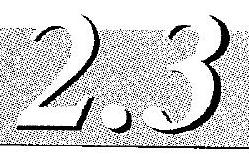
\includegraphics[max width=\textwidth, center]{2024_10_30_21385cc68d0979b6f3f8g-058(1)}

\section{构造相似}
相似三角形可以看作是全等三角形的推广,利用相似三角形不但可以证明角、线段的等量关系,而且还可以证明有关线段的比例关系。利用题中有关相似形的结论、性质,或添线"制造"相似形加以利用,往往是解题的关键所在。

例1 已知 $M 、 N$ 分别在正方形 $A B C D$ 的边 $D A 、 A B$ 上,且 $A M=A N$ ,过 $A$ 作 $B M$ 的垂线,垂足为 $P$ 。求证: $\angle A P N=\angle B N C$ 。

【分析】易知 $\angle B N C=\angle B P C$ ,故只需证 $\angle A P N=\angle B P C$ ,这可通过判定三角形相似来完成。

【证明】连结 $P C$ ,在 Rt $\triangle A B M$ 中, $A P \perp B M$ 。\\
所以 $\angle 1=\angle 2, \angle A P M=\angle B P A=90^{\circ}, \angle 3=$ $\angle 4$, 故 $\triangle A P M \backsim \triangle B P A$. 从而 $\frac{A M}{A B}=\frac{A P}{B P}$.

因为 $A B=B C, A M=A N$, 故 $\frac{A N}{B C}=\frac{A P}{B P}$.\\
因为 $A D / / B C$, 所以 $\angle 4=\angle 5$, 从而 $\angle 3=\angle 5$,\\
所以 $\triangle A P N \backsim \triangle B P C$ ,故 $\angle A P N=\angle B P C ,$\\
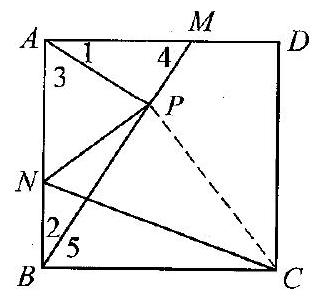
\includegraphics[max width=\textwidth, center]{2024_10_30_21385cc68d0979b6f3f8g-058}

图2-3-1\\
$\angle A N P=\angle B C P$ ,故 $N 、 B 、 C 、 P$ 四点共圆。

进而 $\angle B P C=\angle B N C$ ,所以 $\angle A P N=\angle B N C 。$\\
【注】通过已有相似三角形和线段等量转换,构造新的相似三角形,是解题的关键。

例2 如图 2-3-2:设点 $O$ 是四边形 $A B C D$ 对角线 $A C 、 B D$ 的交点,且 $\frac{B O}{D O}=\frac{7}{6}$ 。若 $\angle B A D+$ $\angle B C A=180^{\circ}, A B=6, A C=5, A D=4$. 求 $B C$的值.

【分析】构造 $\angle B A D$ 或 $\angle B C A$ 的补角,进而得到相等的角,再得到相似三角形去求解。\\
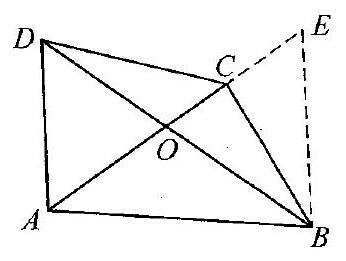
\includegraphics[max width=\textwidth, center]{2024_10_30_21385cc68d0979b6f3f8g-058(2)}

图 2-3-2

【解】过 $B$ 作 $A D$ 的平行线,交 $A C$ 的延长线于

点 $E$.

则 $\angle B A D+\angle A B E=180^{\circ}$ 。\\
因为 $\angle B A D+\angle B C A=180^{\circ}$, 故 $\angle A B E=\angle B C A$.\\
又因为 $\angle B A C=\angle E A B$, 所以 $\triangle B A C \backsim \triangle E A B$.\\
故 $\frac{B C}{B E}=\frac{A C}{A B}=\frac{5}{6}$, 又因为 $A D / / B E$, 从而 $\frac{B E}{A D}=\frac{B O}{D O}=\frac{7}{6}$.\\
所以 $B E=\frac{14}{3}, B C=\frac{35}{9}$.\\
【注】在处理有关线段比例关系时,常常构造平行线和相似三角形来求解。

例3 如图 2-3-3:在等边三角形 $A B C$ 的边 $B C$ 上取一点 $D$ ,使 $C D=$ $2 B D$ ,作 $C H \perp A D, H$ 为垂足,连结 $B H$ 。求证: $\angle D B H=\angle D A B$ 。

【分析】若 $\angle D B H=\angle D A B$ ,则有 $\triangle A B D \backsim \Omega$ $\triangle B H D$ ,需通过边的比例关系计算可得: $B D^{2}=$ $D H \cdot A D$ 。故可相应地作高构造相似三角形求解。

【证明】过 $A$ 作 $A E \perp B C$ ,垂足为 $E$ 。\\
因为 $A E \perp B C, C H \perp A D$ ,所以 $\angle A E D=$ $\angle C H D$ 。

又因为 $\angle C D H=\angle A D E$ ,故 $\triangle C D H \backsim$\\
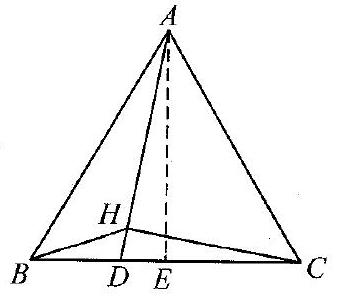
\includegraphics[max width=\textwidth, center]{2024_10_30_21385cc68d0979b6f3f8g-059}

图 2-3-3\\
$\triangle A D E$ 。

从而 $\frac{C D}{A D}=\frac{D H}{D E}$, 即 $A D \cdot D H=C D \cdot D E$.\\
结合 $A B=A C, A E \perp B C$ 可知, $B E=C E$.\\
设 $D E=a$, 则 $B D=2 a, C D=4 a$, 从而 $D E \cdot C D=4 a^{2}=B D^{2}$.\\
故 $\frac{A D}{B D}=\frac{B D}{D H}$, 且 $\angle B D H=\angle A D B$, 进而 $\triangle A D B \backsim \triangle B D H$.\\
故 $\angle D B H=\angle D A B$ 。\\
【注】直接计算法,是构造相似三角形的重要方法之一.\\
例 4 如图 2-3-4:设 $S$ 为锐角 $\triangle A B C$ 的边 $A B$ 上的点, $P 、 Q$ 分别为 $\triangle A S C$ 和 $\triangle B S C$ 的外接圆的圆心。试问:点 $S$ 在边 $A B$ 上的什么位置时,可使 $\triangle P Q S$ 的面积最小?

【分析】利用外心的性质,可得 $\triangle P Q S \backsim$ $\triangle A B C$ ,通过相似比比较两者的面积关系,进而找出最值情况。\\
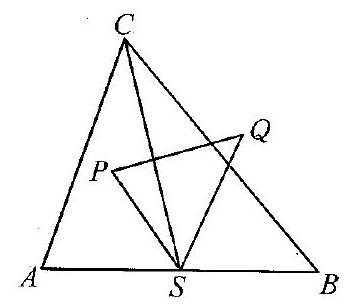
\includegraphics[max width=\textwidth, center]{2024_10_30_21385cc68d0979b6f3f8g-059(1)}

图2-3-4

【解】由题意可知 $P Q$ 垂直平分 $C S$, 故\\
\begin{align*}
\angle S P Q=\frac{1}{2} \angle S P C=\angle S A C=\angle B A C .
\end{align*}

同理: $\angle S Q P=\angle A B C$, 故 $\triangle S Q P \backsim \triangle C B A$.\\
设相似比 $\frac{P S}{A C}=k$. 则 $S_{\triangle P Q S}=k^{2} S_{\triangle A B C}$.\\
又因为 $A C$ 是以 $P S$ 为半径的圆的弦,所以 $A C \leqslant 2 P S$ ,从而 $k \geqslant \frac{1}{2}$ 。\\
故当且仅当 $A C$ 为圆 $P$ 的直径,即 $C S \perp A B$ 时,等号成立。\\
因此点 $S$ 为过点 $C$ 的高线的垂足时, $\triangle P Q S$ 的面积最小, 为 $\frac{1}{4} S_{\triangle A B C}$.\\
【注】利用相似三角形的性质,可将原三角形边、角、周长、面积等问题转换到新的图形中去研究,发现新的思路。

例5 如图 2-3-5:从 $\odot O$ 外的一点 $P$ 作 $\odot O$ 的两条切线, 切点分别为点 $A 、 B$, 在劣弧 $\overparen{A B}$ 上任取一点 $C$,先过点 $C$ 作 $\odot O$ 的切线,分别交 $P A 、 P B$ 于点 $D 、 E$ ,再过点 $C$ 作 $C F \perp A B$, 垂足为 $F$. 求证: $\angle C F D=\angle C F E$ 。

【分析】只需证 $\angle D F A=\angle E F B$, 即有 $\triangle A D F \backsim$ $\triangle B E F$ 。通过作 $A F 、 B F$ 边上的高构造直角三角形相似,再通过边的转换进而求证。

【证明】分别过点 $D 、 E$ 作 $D M \perp A B, E N \perp A B$,垂足为 $M 、 N$ 。\\
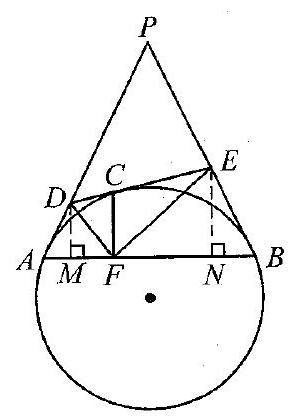
\includegraphics[max width=\textwidth, center]{2024_10_30_21385cc68d0979b6f3f8g-060}

图 2-3-5

故 $\angle A M D=\angle F M D=\angle E N F=\angle E N B=90^{\circ}$ 。\\
因为 $P A=P B$, 所以 $\angle D A M=\angle E B N$ 。\\
从而 $\triangle A D M \backsim \triangle B E N$. 进而 $\frac{D M}{E N}=\frac{A D}{B E}$.\\
由题意: $A D=C D, C E=B E$, 故 $\frac{D M}{E N}=\frac{D C}{C E}$.\\
由题意易知: $D M / / C F / / E N$, 所以 $\frac{D C}{E C}=\frac{M F}{F N}$.\\
故 $\frac{D M}{E N}=\frac{M F}{F N}$, 从而 $\triangle D M F \backsim \triangle E N F$. 进而 $\angle D F M=\angle E F N$.\\
所以 $\angle C F D=\angle C F E$.\\
【注】对于复杂的三角形相似问题,可通过作高,变为直角三角形相似的问题。

例6 如图 2-3-6:在 $\triangle A B C$ 中,设 $A H=$ $B I=\frac{1}{m} A B, B D=C E=\frac{1}{m} B C, C F=A G=$ $\frac{1}{m} A C(m>2) . A D$ 与 $B G$ 交于点 $P, B F$ 与 $C I$ 交于点 $R, A E$ 与 $C H$ 交于点 $Q$. 求证: $\frac{S_{\triangle R Q P}}{S_{\triangle A B C}}=$ $\left(\frac{m-2}{2 m-1}\right)^{2}$.\\
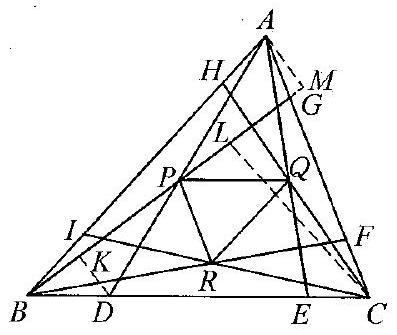
\includegraphics[max width=\textwidth, center]{2024_10_30_21385cc68d0979b6f3f8g-061(1)}

图2-3-6

【分析】可通过比例关系求得 $\triangle P Q R$ 和 $\triangle A B C$ 相似,进而得出面积的比.\\
【证明】分别过 $D 、 C 、 A$ 作 $B G$ 的垂线,垂足分别为 $K 、 L 、 M$ ,从而 $D K / / C L / / A M$ ,故\\
\begin{align*}
\begin{aligned}
\frac{A P}{P D} & =\frac{A M}{D K}=\frac{A M}{B D \cdot \sin \angle G B C} \\
& =\frac{A M}{\frac{1}{m} B C \cdot \sin \angle G B C}=m \cdot \frac{A M}{C L} \\
& =m \cdot \frac{A G}{G C}=\frac{m}{m-1}
\end{aligned}
\end{align*}

同理可证: $\frac{A Q}{Q E}=\frac{m}{m-1}$, 故 $\frac{A P}{P D}=\frac{A Q}{Q E}$, 所以 $P Q / / B C$.\\
同理可证: $P R / / A C 、 Q R / / A B$, 从而 $\triangle P Q R \backsim \triangle C B A$.\\
因为 $\frac{P Q}{B C}=\frac{P Q}{\frac{m}{m-2} D E}=\frac{m-2}{m} \cdot \frac{P Q}{D E}=\frac{m-2}{m} \cdot \frac{A P}{A D}=\frac{m-2}{m} \cdot \frac{1}{1+\frac{P D}{A P}}$\\
\begin{align*}
=\frac{m-2}{m} \cdot \frac{1}{1+\frac{m-1}{m}}=\frac{m-2}{2 m-1},
\end{align*}

故 $\frac{S_{\triangle R Q P}}{S_{\triangle A B C}}=\left(\frac{m-2}{2 m-1}\right)^{2}$.\\
【注】如果两个角的两条边互相平行,则这两个角相等或互补。如果三角形的三条边互相平行,则这两个三角形相似。本题还可以用 Menelaus 定理处理线段的比值,请读者一试。

例7 如图 2-3-7:在锐角 $\triangle A B C$ 中, $A B>$ $A C, M$ 为 $B C$ 的中点, $P$ 在 $\triangle A M C$ 内, 且 $\angle B A M=$ $\angle P A C$, 设 $\triangle A B C 、 \triangle A B P 、 \triangle A C P$ 的外心分别为 $O 、 O_{1} 、 O_{2}$. 求证: $A O$ 平分 $O_{1} O_{2}$ 。\\
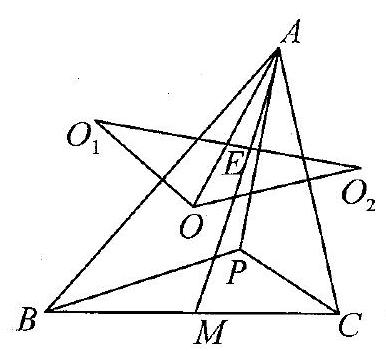
\includegraphics[max width=\textwidth, center]{2024_10_30_21385cc68d0979b6f3f8g-061}

图2-3-7

【分析】易知 $\angle A O O_{2}=\angle A B C$ ,再结合条件可得 $\angle O_{2}=\angle B A M$ 。通过相似由 $M$ 为 $B C$ 中点,可证得 $E$ 为 $O_{1} O_{2}$ 中点。

【证明】因为 $O_{1} 、 O_{2}$ 分别为 $\triangle A B P$ 和 $\triangle A C P$ 的外心,所以 $O_{1} O_{2} \perp A P$ 。同理: $O O_{2} \perp A C$ ,故 $\angle O_{2}=\angle P A C$ 。\\
又因为 $\angle B A M=\angle P A C$, 所以 $\angle O_{2}=\angle B A M$.\\
因为 $O$ 为 $\triangle A B C$ 的外心,所以 $\angle O_{2} O E=\angle A B M$ ,进而 $\triangle O_{2} O E \backsim \triangle A B M$ 。\\
同理: $\triangle O_{1} O E \backsim \triangle A C M$ ,故 $\frac{O_{1} E}{O E}=\frac{A M}{C M}, \frac{A M}{B M}=\frac{O_{2} E}{O E}$ 。\\
因为 $B M=C M$ ,故 $O_{1} E=O_{2} E$ ,即 $A O$ 平分 $O_{1} O_{2}$ 。\\
【注】可构造 $\triangle A B C$ 的外接圆,将 $\angle B A M$ 和 $\angle C A M$ 转换成新的圆周角,直接构造三角形和 $\triangle O_{1} O_{2} O$ 相似。

【证明】延长 $A M$ 交 $\triangle A B C$ 外接圆于 $D$ ,连结 $B D 、 C D$ 。

由上面证明可知:\\
\begin{align*}
\begin{aligned}
& \angle O_{1}=\angle M A C=\angle C B D \\
& \angle O_{2}=\angle B A M=\angle B C D
\end{aligned}
\end{align*}

从而 $\triangle O_{1} O_{2} O \backsim \triangle B C D$ 。\\
由上面证明可证: $\triangle O E O_{2} \backsim \triangle D M C$ , $\triangle O E O_{1} \backsim \triangle D M B$ 。\\
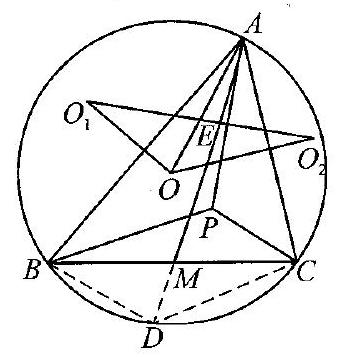
\includegraphics[max width=\textwidth, center]{2024_10_30_21385cc68d0979b6f3f8g-062(2)}

图2-3-8

进而 $\frac{O_{1} E}{B M}=\frac{O_{1} O}{B D}=\frac{O_{1} O_{2}}{B C}$.\\
因为 $B M=\frac{1}{2} \dot{B} C$, 故 $O_{1} E=\frac{1}{2} O_{1} O_{2}$, 即 $A O$ 平分 $O_{1} O_{2}$.

\section{练 习 2.3}
1 如图:已知在 $\triangle A B C$ 中, $\angle B A C=90^{\circ}, A D \perp B C, E$ 是 $A C$ 的中点, $E D$的延长线交 $A B$ 的延长线于 $F$. 求证: $\frac{A B}{A C}=\frac{D F}{A F}$.\\
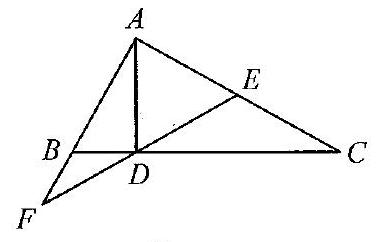
\includegraphics[max width=\textwidth, center]{2024_10_30_21385cc68d0979b6f3f8g-062(1)}\\
(第1题)\\
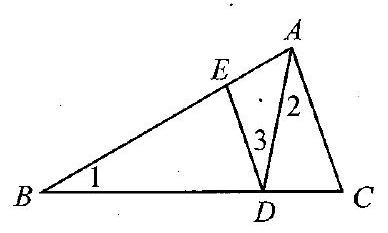
\includegraphics[max width=\textwidth, center]{2024_10_30_21385cc68d0979b6f3f8g-062}\\
(第2题)

2 . 如图:在 $\triangle A B C$ 中, $B C=a, A C=b, A B=c, D 、 E$ 分别是边 $B C 、 A B$上的点,且 $\angle 1=\angle 2=\angle 3$ ,如果 $\triangle A B C 、 \triangle E B D 、 \triangle A D C$ 的周长依次为 $m 、 m_{1} 、 m_{2}$ 。求证: $\frac{m_{1}+m_{2}}{m} \leqslant \frac{5}{4}$.\\
際 如图:四边形 $A B C D$ 是梯形,点 $E$ 是上底边 $A D$ 上一点, $C E$ 的延长线与 $B A$ 的延长线交于点 $F$ ,过点 $E$ 作 $B A$ 的平行线交 $C D$ 的延长线于点 $M, B M$ 与 $A D$ 交于点 $N$. 证明: $\angle A F N=$ $\angle D M E$ 。\\
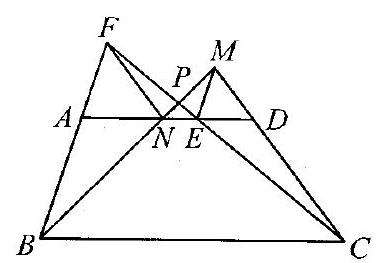
\includegraphics[max width=\textwidth, center]{2024_10_30_21385cc68d0979b6f3f8g-063(4)}\\
(第3题)

4 如图:直线 $m$ 的同侧有三个相邻的等边 $\triangle A B C 、 \triangle A D E 、 \triangle A F G$ ,且 $G$ 、 $A 、 B$ 都在直线 $m$ 上,设这个三角形的边长依次为 $a 、 b 、 c$ ,连结 $G D$ 交 $A E$ 于 $N$ ,再连结 $B N$ 交 $A C$ 于 $L$ 。求 $A L$ 。\\
\includegraphics[max width=\textwidth, center]{2024_10_30_21385cc68d0979b6f3f8g-063(1)}\\
(第4题)\\
\includegraphics[max width=\textwidth, center]{2024_10_30_21385cc68d0979b6f3f8g-063(2)}\\
(第 $\mathbf{5}$ 题)

医如图:在 $\triangle A B C$ 中, $\angle A$ 是直角, $A D \perp B C$ 于 $D, A T$ 平分 $\angle B A C, O_{1}$ 、 $O_{2}$ 分别是 $\triangle A B D$ 和 $\triangle A C D$ 的内心。证明: $A T \perp O_{1} O_{2}$ 。\\
6. 如图:在 $\triangle A B C$ 中, $\angle A C B=90^{\circ}$ ,点 $D$ 在 $C A$ 上,使得 $C D=1, A D=3$ ,并且 $\angle B D C=3 \angle B A C$. 求 $B C$ 的长.\\
(7) 设 $T=(a, b, c)$ 是一个边长为 $a, b, c$ 的三角形,其面积为 $\triangle$ ;记 $T^{\prime}=\left(a^{\prime}, b^{\prime}, c^{\prime}\right)$\\
\includegraphics[max width=\textwidth, center]{2024_10_30_21385cc68d0979b6f3f8g-063}\\
(第 6 题)

是由原三角形 $T$ 的三条高组成的三角形, $T^{\prime}$ 的面积记为 $\triangle^{\prime}$ ;进一步,记 $T^{\prime \prime}=\left(a^{\prime \prime}, b^{\prime \prime}, c^{\prime \prime}\right)$ 是由原三角形 $T^{\prime}$ 的三条高组成的三角形, $T^{\prime \prime}$ 的面积记为 $\triangle^{\prime \prime}$ 。已知 $\triangle^{\prime}=30, \triangle^{\prime \prime}=20$ ,求 $\triangle$ 的值。\\
8 如图:已知三个彼此相似的三角形 $\triangle, \triangle_{1}, \triangle_{2}$,它们的周长分别为 $p, p_{1}, p_{2}$ ,若较小的两个三角形 $\triangle_{1}$ 和 $\triangle_{2}$ 可以互不重叠地放在大三角形 $\triangle$ 的内部。求证: $p_{1}+p_{2}<\sqrt{2} p$ 。\\
\includegraphics[max width=\textwidth, center]{2024_10_30_21385cc68d0979b6f3f8g-063(3)}\\
(第8题)

9 不等边 $\triangle A B C$ 的三边长为 $a 、 b 、 c$, 且 $a+b=2 c$, 若经过 $\triangle A B C$ 的重心

夏门郑剑雄高中数学竞赛系列\\
全国小学奥数群:221739457,全国初中奥数学生群:253736211,全国高中奥数学生群591782992全国初中奥数教练群112464128,全国高中奥数教练群195949359竞赛公众号:新浪微博@郑剑雄 微信:v136257437 QQ:136257437\\
业务:初高中联赛班、培优班、美国高中数学、教师培训、机构教学产品研发、讲义资料出售等\\
$G$ 和内心 $I$ 的直线分该三角形两部分的面积为 $S_{1}$ 和 $S_{2}\left(S_{1} \leqslant S_{2}\right)$. 求 $\frac{S_{1}}{S_{2}}$的值。\\
10 如图:已知 $D$ 为 $\triangle A B C$ 的边 $B C$ 上的任意一点, $I_{1} 、 I_{2}$ 分别为 $\triangle A B D 、 \triangle A C D$ 的内心, $I_{1}^{\prime} 、$ $I_{2}^{\prime}$ 分别为这两个三角形的旁心, $P 、 P^{\prime}$ 分别为 $\triangle A B C$ 的内切圆和旁切圆与边 $B C$ 的切点。证明: $\triangle I_{1} P I_{2} \circlearrowright \triangle I_{2}^{\prime} P^{\prime} I_{1}^{\prime}$ 。\\
\includegraphics[max width=\textwidth, center]{2024_10_30_21385cc68d0979b6f3f8g-064}\\
(第 10 题)

圆与直线型可组合成一些复杂的几何图形,是一类综合性的几何问题。利用圆的性质,可以丰富几何计算和几何证明的方法。在本节中,我们对圆的有关典型问题作一个简单的介绍。

例1 如图 2-4-1:四边形 $A B C D$ 内接于圆 $O, A D$ 为直径,且 $A D=8$ , $A B=B C, C D=7$, 求 $A B$ 的长.

【分析】利用条件 $A B=B C$ ,则可推出所对圆周角相等,故构建出代数方程求解。

【解】设 $A B=B C=x, B D=y$ 。\\
且 $\angle A D B=\angle B D C=\alpha$ 。\\
则由余弦定理得:\\
\includegraphics[max width=\textwidth, center]{2024_10_30_21385cc68d0979b6f3f8g-065}

图2-4-1\\
\begin{align*}
\cos \alpha=\frac{8^{2}+y^{2}-x^{2}}{2 \times 8 y}=\frac{7^{2}+y^{2}-x^{2}}{2 \times 7 y}
\end{align*}

故 $y^{2}=x^{2}+56$ 。\\
因为 $A D$ 为 $\odot O$ 直径, 故 $\angle A B D=90^{\circ}$. 从而 $y^{2}+x^{2}=64$, 故 $x=2$, 即 $A B=2$ 。

注意到 $\overparen{A B}=\overparen{B C}$ 这个条件,还可以考虑使用垂径定理。

【解】连结 $A C, B O$ 交于点 $M$.\\
因为 $A B=B C$ ,所以 $\overparen{A B}=\overparen{B C}$ 。\\
又因为 $B O$ 为半径,所以 $B O \perp A C$ 。\\
\includegraphics[max width=\textwidth, center]{2024_10_30_21385cc68d0979b6f3f8g-065(1)}

图2-4-2

因为 $A D$ 为 $\odot O$ 的直径,因此 $C D \perp A C$ 。\\
从而 $M O / / C D$, 所以 $M O=\frac{1}{2} C D=\frac{7}{2}, B M=\frac{1}{2}$.\\
在 Rt $\triangle A M O$ 中, $A M^{2}=4^{2}-\left(\frac{7}{2}\right)^{2}=\frac{15}{4}$.

在 Rt $\triangle A B M$ 中, $A B^{2}=\frac{15}{4}+\left(\frac{1}{2}\right)^{2}=4$, 即 $A B=2$ 。\\
注意到垂直和角平分线,还可以构造等腰三角形来求解。\\
【解】如图2-4-3连结 $B D$ ,延长 $A B$ 和 $D C$交于点 $E$ 。

由前面解法可得: $\triangle A B D \cong \triangle E B D$ 。\\
故 $E B=A B=B C=x, A D=E D=8$, $E C=1$ 。\\
\includegraphics[max width=\textwidth, center]{2024_10_30_21385cc68d0979b6f3f8g-066(1)}

图2-4-3

故由割线定理: $E B \cdot E A=E C \cdot E D$ 。\\
故 $2 x^{2}=8, x=2$ ,即 $A B=2$ 。\\
【注】在解决有关圆的问题中,要善于结合圆的性质和其他图形性质,运用多种方法思考。

例2 如图 2-4-4: $A B$ 为 $\odot O$ 的直径, $C$ 为半圆弧 $A B$ 上一点, $C D \perp$ $A B$ 于 $D$ ,以 $C$ 为圆心, $C D$ 的长为半径的圆交 $\odot O$ 于点 $E 、 F$ 。求证: $E F$ 平分 $C D$ 。

【分析】 $E F$ 为 $\odot O$ 和 $\odot C$ 的公共弦,可考虑分别在两圆中以 $E F$ 为弦使用相交弦定理,寻找所要的数量关系。

【证明】延长 $C D$ 和 $D C$ ,分别交 $\odot O$ 和 $\odot C$于 $M 、 N$ 点。

由相交弦定理得:CG $\cdot$ GM = EG $\cdot$ GF, $D G \cdot G N=E G \cdot G F$.

故 $C G \cdot G M=D G \cdot G N$.\\
\includegraphics[max width=\textwidth, center]{2024_10_30_21385cc68d0979b6f3f8g-066}

图2-4-4

从而 $C G \cdot(D G+M D)=D G \cdot(C G+C N)$.\\
进而 $C G \cdot M D=D G \cdot C N$ 。\\
结合 $A B \perp C D$ 且 $A B$ 为直径,故 $M D=C D$ 。\\
由于 $C D=C N$ ,所以 $C G=D G$ ,即 $E F$ 平分 $C D$ 。\\
【注】圆不仅是中心对称图形,而且还是轴对称图形,过圆心的直线是它的对称轴。利用圆的对称性可帮助我们解决问题。

例3 如图 2-4-5: $A B$ 为 $\odot O$ 的直径, $A B=2 R$ , $C D$ 为一条动弦, $C D$ 交 $A B$ 于 $E$ ,且 $\angle A E C=45^{\circ}$ 。求证: $C E^{2}+E D^{2}$ 为定值。

【分析】利用圆的对称性,构造直角三角形,简化 $C E^{2}+E D^{2}$ 。

【证明】过 $C$ 点作关于 $A B$ 的对称点 $F$, 连结 $E F$ 、\\
\includegraphics[max width=\textwidth, center]{2024_10_30_21385cc68d0979b6f3f8g-066(2)}

图2-4-5\\
$D F$ ,则点 $F$ 在 $\odot O$ 上.\\
由圆的对称性: $C E=F E, \angle C E F=2 \angle C E A=90^{\circ}$, 故 $\angle F E D=90^{\circ}$.\\
从而 $C E^{2}+E D^{2}=E F^{2}+E D^{2}=F D^{2}$ 。\\
由正弦定理得: $F D=2 R \sin \angle F C D$ 。\\
故 $F D=\sqrt{2} R$ 。\\
所以 $C E^{2}+E D^{2}=2 R^{2}$ 为定值。\\
【注】在处理平面几何中的许多问题时,常常需要借助于圆的性质,但常常我们直接要用的圆并不存在,这就需要我们利用已知条件,借助图形把实际存在的圆找出来,再利用这个圆的性质解题。

例4 如图 2-4-6: $P A 、 P B$ 分别切 $\odot O$ 于点 $A 、 B, O P$ 交 $A B$ 于点 $C$,弦 $E F$ 过点 $C$. 求证: $\angle A P E=\angle B P F$.

【分析】 $\angle A P E$ 和 $\angle B P F$ 对于 $\odot O$ 而言均为圆外角,直接证明不容易。考虑到问题等价于 $\angle E P O=\angle F P O$ ,若证明 $O 、 F 、 P$ 、 $E$ 四点共圆,再结合 $O E=O F$ 即可。

【证明】连结 $O E 、 O F 、 O A 、 O B$ 。\\
因为 $P A$ 切 $\odot O$ 于 $A 、 P B$ 切 $\odot O$ 于 $B$, 所以 $O A \perp P A, O B \perp P B$ ,从而 $A 、 P 、 B 、 O$ 四\\
\includegraphics[max width=\textwidth, center]{2024_10_30_21385cc68d0979b6f3f8g-067}

图2-4-6

点共圆。

故 $O C \cdot P C=A C \cdot B C$.\\
因为 $E C \cdot F C=A C \cdot B C$ ,故 $O C \cdot P C=E C \cdot F C$ 。\\
进而 $E 、 O 、 F 、 P$ 四点共圆,故 $\angle 1=\angle 4, \angle 2=\angle 3$ ,因为 $O E=O F$ ,故 $\angle 1=\angle 2$ ,从而 $\angle 3=\angle 4$ 。

因为 $\angle A P O=\angle B P O$ ,所以 $\angle A P E=\angle B P F$ 。\\
【注】判断四点共圆的主要依据和方法有:\\
(1)四边形的一组对角互补,那么这个四边形的四个顶点共圆。\\
(2)四边形的一个外角等于它的内对角,那么这个四边形的四个顶点共圆。\\
(3)线段向同侧所张的两个角相等,那么两个角的顶点和线段的端点共圆。\\
(4)四边形的两条对角线交点分每条对角线所成的两段线段之积相等,那么这个四边形的四个顶点共圆。\\
(5)延长四边形的一组对边相交于一点,若这点到这组对边中每一边端点的两条线段长的积相等,那么这个四边形的四个顶点共圆。\\
(6)到同一个点距离相等的四个点共圆。

例5 如图 2-4-7: $\triangle A B C$ 的内切圆分别切 $A B 、 A C$ 于点 $E 、 F, D$ 是 $B C$的中点, $\angle B 、 \angle C$ 的平分线分别与直线 $E F$ 交于点 $N 、 M$ 。证明: $D M=D N$ 。

【分析】若 $\triangle B M C$ 和 $\triangle B N C$ 均为直角三角形即证,故可考虑证 $B 、 E 、 M 、 I$ 四点共圆及 $C 、 F 、 N 、 I$四点共圆。

【证明】设 $\triangle A B C$ 内心为 $I$, 连结 $A I 、 E I 、 F I$ 、 $B M 、 C N$ 。

由题意得: $A 、 E 、 I 、 F$ 四点共圆,故\\
\begin{align*}
\angle I E F=\angle I A F=\frac{1}{2} \angle A
\end{align*}\\
\includegraphics[max width=\textwidth, center]{2024_10_30_21385cc68d0979b6f3f8g-068}

图 2-4-7

进而 $\angle B E M=90^{\circ}+\angle I E F=90^{\circ}+\frac{1}{2} \angle A=\angle B I C$,\\
所以 $B 、 E 、 M 、 I$ 四点共圆。\\
故 $\angle B M I=\angle B E I=90^{\circ}$ ,即 $\triangle B M C$ 为直角三角形。\\
因为 $D$ 是 $B C$ 的中点, 所以 $D M=\frac{1}{2} B C$.\\
同理: $D N=\frac{1}{2} B C$ ,故 $D M=D N$ 。\\
【注】在题目中涉及三角形的外心或内心时,还可以构造三角形的外接圆或内切圆帮助解题。

例6 在 $\triangle A B C$ 中, 已知点 $I$ 为内心, 点 $O$ 为外心, $A B=5, B C=6$, $C A=4$. 求证 $: O I \perp C I$ 。

【分析】构造 $\triangle A B C$ 的外接圆, 证明点 $I$ 是 $E C$ 中点即可。

【证明】延长 $C I$ 交 $A B$ 于点 $D$, 交 $\triangle A B C$ 的外接圆于点 $E$.

因为 $C I$ 平分 $\angle A C B$, 所以 $\frac{A C}{B C}=\frac{A D}{B D}=\frac{2}{3}$.\\
结合 $A B=5$, 可得 $A D=2, B D=3$ 。\\
\includegraphics[max width=\textwidth, center]{2024_10_30_21385cc68d0979b6f3f8g-068(1)}

图2-4-8

由角平分线长公式: $C D^{2}=A C \cdot B C-A D \cdot B D$得, $C D=3 \sqrt{2}$ 。

由于 $A D \cdot B D=C D \cdot E D$ ,故 $E D=\sqrt{2}$ 。\\
又因为 $\frac{A D}{A C}=\frac{D I}{I C}=\frac{D I}{3 \sqrt{2}-D I}$, 故 $D I=\sqrt{2}$.\\
从而 $E I=I C=2 \sqrt{2}$, 所以 $O I \perp E C$.

例7 如图 2-4-9: $\triangle A B C$ 外接圆的圆心为 $O$, 点 $P 、 Q$ 分别在线段 $C A 、 A B$ 上, $K 、 L 、 M$ 分别是 $B P 、 C Q 、 P Q$ 的中点, 圆 $O$ 过 $K 、 L 、 M$ 并且与 $P Q$ 相切。证明: $O P=O Q$ 。

【分析】若 $P O=Q O$ ,即 $P 、 Q$ 关于 $\odot O$ 等幕,需证 $A Q \cdot Q B=A P \cdot P C$. 考虑到中点,可从构造中位线入手。

【证明】 连结 $M K, K L, M L$, 因为 $P Q$ 与 $\odot O$ 相切,所以 $\angle K M Q=\angle K L M$.

又因为 $M K$ 为 $\triangle B P Q$ 的中位线, 因此 $M K / /$ $B Q$ 。

因为 $\angle K M Q=\angle A Q P$, 故 $\angle K L M=$ $\angle A Q P$ 。\\
\includegraphics[max width=\textwidth, center]{2024_10_30_21385cc68d0979b6f3f8g-069(2)}

图2-4-9

同理: $\angle L K M=\angle A P Q$, 从而 $\triangle A P Q \backsim \triangle M K L$.\\
故 $\frac{A P}{M K}=\frac{A Q}{M L}$.\\
因为 $M K=\frac{1}{2} B Q, M L=\frac{1}{2} P C$ ,所以 $\frac{A P}{B Q}=\frac{A Q}{P C}$.\\
即 $A P \cdot P C=A Q \cdot B Q$ ,故 $P 、 Q$ 关于 $\odot O$ 等幂。\\
所以 $O P=O Q$.

1胃: $\triangle A B C$ 的外接圆圆心为 $O$ ,以 $B C$ 边为直径的 $\odot O^{\prime}$ 交 $A B$ 于点 $E$ ,交 $A C$ 于点 $D$, 若 $E D$ 的中点为点 $F$. 求证: $O A / / O^{\prime} F$ 。\\
\includegraphics[max width=\textwidth, center]{2024_10_30_21385cc68d0979b6f3f8g-069}\\
(第1题)\\
\includegraphics[max width=\textwidth, center]{2024_10_30_21385cc68d0979b6f3f8g-069(1)}\\
(第2 题)

2 如图:在 $\triangle A B C$ 中, $D 、 E 、 F$ 分别为 $A B 、 B C 、 A C$ 边的中点,分别作 $\triangle A B C$ 与 $\triangle D E F$ 的外接圆 $\odot O$ 与 $\odot O^{\prime}$, 过 $A$ 作圆 $O$ 的切线, 过点 $E$ 作\\
$\odot O^{\prime}$ 的切线. 求证: $M N / / G H$ 。\\
3 如图:圆内接四边形 $A B C D, A B=A D$ , $P B=B O, C E \perp P E, C D=18$, 求 $D E$的长.\\
4 圆内接四边形 $A B C D$ 的对角线 $A C 、 B D$ 相交于点 $E$, 线段 $B C=D C=4, A E=6, B E$\\
\includegraphics[max width=\textwidth, center]{2024_10_30_21385cc68d0979b6f3f8g-070(4)}\\
(第3题)

和 $D E$ 的长都是正整数,求 $B D$ 的长。\\
蛊如图: $A B$ 为 $\odot O$ 的直径, 自 $A B$ 上一点 $C$ 向圆的切线 $D F$ 作垂线 $C F, F$为垂足, $D$ 为切点, $D E$ 为过 $C$ 的弦, 若 $C F=8, C D=10, A B=14$. 求 $C E$ 的长。\\
\includegraphics[max width=\textwidth, center]{2024_10_30_21385cc68d0979b6f3f8g-070(2)}\\
(第 5 题)\\
\includegraphics[max width=\textwidth, center]{2024_10_30_21385cc68d0979b6f3f8g-070}\\
(第 6 题)

6 如图: 直线 $A B$ 和 $A C$ 与圆 $O$ 分别相切于 $B 、 C$ 两点, $P$ 为圆上一点, 且 $P$到 $A B 、 A C$ 的距离分别为 6 和 4 , 求点 $P$ 到 $B C$ 的距离.\\
雷设 $C$ 为平面上一个圆, 而 $C_{1}, C_{2}$ 是两个没有交点的圆, 它们都内切于 $C$,切点分别为 $A 、 B$. 直线 $t$ 为 $C_{1}, C_{2}$ 的一条公切线, 分别切 $C_{1}, C_{2}$ 于点 $D 、 E$, 且圆 $C_{1}, C_{2}$ 在 $t$的同一侧. $F$ 为 $A D$ 和 $B E$ 的交点。证明:点 $F$ 在圆 $C$ 上.\\
8 . 如图: 在 $\triangle A B C$ 中, 已知 $A D \perp B C, B E \perp C A$, $A D$ 与 $B E$ 相交于点 $H, P$ 为边 $A B$ 的中点, 过点 $C$ 作 $C Q \perp P H$, 垂足为 $Q$. 求证: $P E^{2}=$ $P H \cdot P Q$.\\
5 已知点 $O$ 是锐角 $\triangle A B C$ 的外心,过 $A 、 B 、 O$ 三点的圆交 $A C 、 B C$ 于点 $E 、 F$, 且 $E F=O C$. 求证: $O C \perp E F$, 且 $\angle A C B=45^{\circ}$ 。\\
10 如图: 在锐角 $\triangle A B C$ 中, $A B>A C, \angle B A C=$ $60^{\circ}, O 、 H$ 分别为 $\triangle A B C$ 的外心、垂心, 直线 $O H$ 分别与 $A B 、 A C$ 交于点 $P 、 Q$. 求证: $P O=$ QH.\\
\includegraphics[max width=\textwidth, center]{2024_10_30_21385cc68d0979b6f3f8g-070(3)}\\
(第8 题)\\
\includegraphics[max width=\textwidth, center]{2024_10_30_21385cc68d0979b6f3f8g-070(1)}\\
(第 10 题)

在处理几何问题的时候,往往将"形"的问题借助于数式的推理,使之量化,从而具体探索"形"的性质,最终得到相应的几何量之间的关系。

例1 如图 2-5-1:矩形 $A B C D$ 中, $E 、 F$ 为 $B C$ 、 $C D$ 上的点,且 $S_{\triangle A B E}=5, S_{\triangle A D F}=4, S_{\triangle C E F}=3$ 。求 $\triangle A E F$ 的面积。

【分析】已知条件中三个三角形均为直角三角形,可适当引入字母表示面积关系。对于所求不规则 $\triangle A E F$ 的面积,则可通过面积割补来表示。\\
\includegraphics[max width=\textwidth, center]{2024_10_30_21385cc68d0979b6f3f8g-071}

图 2-5-1

【解】设 $A B=a, B C=b$, 则 $B E=\frac{10}{a}, D F=\frac{8}{b}$.\\
故由 $\left(a-\frac{8}{b}\right)\left(b-\frac{10}{a}\right)=6$, 可得 $a b+\frac{80}{a b}=24$.\\
解得: $a b=20$ 或 $a b=4$ (舍),故 $S_{\triangle A E F}=20-5-4-3=8$ 。\\
【注】本题解法是将面积数量化,当然也可从面积的比例关系入手解答。连结 $D E$ ,设 $S_{\triangle D E F}=x$ ,则有 $\frac{x+3}{x+3+5}=\frac{x}{4} , x=2$ ,进而得解。

例2 如图 2-5-2: 四边形 $A B C D$ 是直角梯形,且 $A B=B C=2 A D$ , $P A=1, P B=2, P C=3$, 求梯形 $A B C D$ 的面积。

【分析】本题只需求出高 $A B$ 即可。可考虑将 $\triangle P A B$ 和 $\triangle P B C$ 分解成若干个直角三角形,通过勾股定理来寻求有关 $A B$ 的数量关系。

【解】过 $P$ 作 $P M \perp A B, P N \perp B C$ ,垂足分别为 $M$ 、 $N$. 设 $P M=x, P N=y, A B=m$ ,则由勾股定理得:\\
\begin{align*}
\left\{\begin{array}{l}
x^{2}+y^{2}=4 \\
x^{2}+(m-y)^{2}=1 \\
(m-x)^{2}+y^{2}=9
\end{array}\right.
\end{align*}\\
\includegraphics[max width=\textwidth, center]{2024_10_30_21385cc68d0979b6f3f8g-071(1)}

图2-5-2

由(1)(2)得:\\
\begin{align*}
\begin{aligned}
& y=\frac{m^{2}+3}{2 m} \\
& x=\frac{m^{2}-5}{2 m}
\end{aligned}
\end{align*}

由(1)(3)得:\\
代入(1)得: $m^{4}-10 m^{2}+17=0$, 解得 $m^{2}=5 \pm 2 \sqrt{2}$.\\
因为 $m>y$, 故 $\frac{m^{2}+3}{2 m}<m$, 即 $m^{2}>3$, 故 $m^{2}=5+2 \sqrt{2}$, 故 $A B^{2}=5+$ $2 \sqrt{2}$.\\
\includegraphics[max width=\textwidth, center]{2024_10_30_21385cc68d0979b6f3f8g-072}\\
【注】本题也可利用图形旋转的观点, 将 $\triangle B C P$ 绕点 $B$ 逆时针旋转 $90^{\circ}$后得 $\triangle B A Q$, 可求得 $\angle A P B=135^{\circ}$, 进而求得 $A B$.

例3 在锐角 $\triangle A B C$ 中, $B D$ 是 $A C$ 边上的高, $E$ 是 $A B$ 边上的一点, 满足 $\angle A E C=45^{\circ}, B D=2 C E$, 且 $D E / / B C$. 求证: $C E=A C+A D$.

【分析】利用 $\angle A E C=45^{\circ}$, 可构造等腰直角三角形,再利用 $B D=2 C E$ ,可将图中线段数量化,进而寻找所求的数量关系。

【证明】过点 $C$ 作 $C F \perp A B$, 交 $A B$ 于点 $F$.\\
设 $A D=x, C E=a$, 则 $B D=2 a, A B=\sqrt{4 a^{2}+x^{2}}$.\\
在 $\mathrm{Rt} \triangle C E F$ 中, $\angle C E F=45^{\circ}$, 故 $E F=C F=\frac{\sqrt{2}}{2} a$.\\
由于 Rt $\triangle A C F \backsim \operatorname{Rt} \triangle A B D$ ,从而\\
\begin{align*}
\frac{A F}{A D}=\frac{A C}{A B}=\frac{F C}{B D}=\frac{\frac{\sqrt{2}}{2} a}{2 a}=\frac{\sqrt{2}}{4}
\end{align*}\\
\includegraphics[max width=\textwidth, center]{2024_10_30_21385cc68d0979b6f3f8g-072(1)}

图 2-5-3

故 $A F=\frac{\sqrt{2}}{4} x, A C=\frac{\sqrt{2}}{4} \sqrt{4 a^{2}+x^{2}}$.\\
因为 $D E / / B C$, 所以 $\frac{A D}{A C}=\frac{A E}{A B}$.\\
从而 $A D=\frac{A C}{A B} \cdot A E=\frac{\sqrt{2}}{4}(E F+A F)=\frac{\sqrt{2}}{4}\left(\frac{\sqrt{2}}{4} x+\frac{\sqrt{2}}{2} a\right)$.\\
即 $x=\frac{\sqrt{2}}{4}\left(\frac{\sqrt{2}}{4} x+\frac{\sqrt{2}}{2} a\right)$, 解得 $x=\frac{2}{7} a$.

故 $A C=\frac{5}{7} a$ ,进而 $A C+A D=a=C E$ 。\\
【注】对于线段的和差问题,并不一定采取截长补短法或中线加倍法,通过数的量化往往更有利于思考分析。

例4 如图 2-5-4:在四边形 $A B C D$ 中, $\triangle A B D 、 \triangle B C D 、 \triangle A B C$ 的面积是 $3: 4: 1$, 点 $M 、 N$ 分别在 $A C 、 C D$ 上, 满足 $A M: A C=C N: C D$, 并且 $B 、 M 、 N$ 三点共线。求证: $M$ 与 $N$ 分别是 $A C$ 与 $C D$ 的中点。

【分析】条件中比例关系 $A M: A C=C N: C D$ ,并不能推出平行关系,只有结合结论可知 $A M: A C=$ $C N: C D=m=\frac{1}{2}$ ,故可考虑引入参数 $m$ ,再结合面积的比例关系求解。

【证明】设 $\frac{A M}{A C}=\frac{C N}{C D}=m(0<m<1)$.\\
由共边定理得: $\frac{B E}{E D}=\frac{1}{6}$, 进而 $\frac{B E}{B D}=\frac{1}{7}$.\\
\includegraphics[max width=\textwidth, center]{2024_10_30_21385cc68d0979b6f3f8g-073}

图2-5-4

同理: $\frac{A E}{A C}=\frac{3}{7}$.\\
从而 $\frac{E M}{M C}=\frac{7 m-3}{7-7 m}, \frac{C N}{N D}=\frac{m}{1-m}$.\\
因为 $B 、 M 、 N$ 三点共线,故由梅涅劳斯定理有: $\frac{C N}{N D} \cdot \frac{D B}{B E} \cdot \frac{E M}{M C}=1$, 故 $\frac{m}{1-m} \cdot 7 \cdot \frac{7 m-3}{7-7 m}=1$.

即 $6 m^{2}-m-1=0$, 解得 $m_{1}=\frac{1}{2}, m_{2}=-\frac{1}{3}$ (舍), 所以 $M 、 N$ 分别是 $A C 、 C D$ 的中点.

例5 在 $\triangle A B C$ 中, 已知点 $I$ 为内心, 点 $O$ 为外心, $A B=5, B C=6$, $C A=4$. 求证: $O I \perp C I$ 。

【分析】在上节中,利用 $\triangle A B C$ 的外接圆及垂径定理来证明。本题也可通过线段长度的计算,使用勾股定理逆定理来证明。

【证明】 连结 $C O$, 过点 $I$ 过 $I D \perp C A$ ,垂足为 $D$ 。

由题意: $p=\frac{1}{2}(a+b+c)=\frac{15}{2}$ ( $p$ 为 $\triangle A B C$ 的\\
\includegraphics[max width=\textwidth, center]{2024_10_30_21385cc68d0979b6f3f8g-073(1)}

图2-5-5

周长的一半),故\\
\begin{align*}
S=\sqrt{p(p-a)(p-b)(p-c)}=\frac{15}{4} \sqrt{7}
\end{align*}

因为 $S=p \cdot r$ ( $r$ 为内接圆半径, 即 $I D$ 的长 $)$, 所以 $r=\frac{\sqrt{7}}{2}$.\\
又因为\\
\begin{align*}
C D=\frac{B C+C A-A B}{2}=\frac{5}{2},
\end{align*}

所以\\
\begin{align*}
C I=\sqrt{C D^{2}+I D^{2}}=2 \sqrt{2}
\end{align*}

由余弦定理得:\\
\begin{align*}
\cos \angle A C B=\frac{4^{2}+6^{2}-5^{2}}{2 \times 4 \times 6}=\frac{9}{16}
\end{align*}

进而 $\sin \angle A C B=\frac{5}{16} \sqrt{7}$.\\
由正弦定理得: $2 R=\frac{A B}{\sin \angle A C B}$, 故 $R=\frac{8}{7} \sqrt{7}$, 即外接圆半径 $O C=\frac{8}{7} \sqrt{7}$.\\
由欧拉公式得: $O I^{2}=R^{2}-2 R r$ ,故 $O I^{2}=\frac{8}{7}$ 。\\
从而 $I O^{2}+I C^{2}=O C^{2}$ ,故 $O I \perp C I$ 。\\
例 6 若凸四边形 $A B C D$ 内有一点 $O$ ,且该点到凸四边形各顶点距离的平方和等于凸四边形面积的 2 倍。求证:该凸四边形为正方形。

【分析】显然该命题的逆命题成立。考虑到四边形面积可分成四个小三角形,联系题设中 $O A$ 、 $O B$ 等条件,可利用面积公式 $S=\frac{1}{2} a b \sin \alpha$ 来表示,\\
\includegraphics[max width=\textwidth, center]{2024_10_30_21385cc68d0979b6f3f8g-074}

图 2-5-6

并用不等式进行适当的放缩变换。

【证明】由题意:\\
\begin{align*}
2 S=O A^{2}+O B^{2}+O C^{2}+O D^{2}
\end{align*}

故 $4 S=2\left(O A^{2}+O B^{2}+O C^{2}+O D^{2}\right)$.\\
故 $4 S \geqslant 2 O A \cdot O B+2 O B \cdot O C+2 O C \cdot O D+2 O D \cdot O A$.\\
故 $4 S \geqslant 2 \sin \angle A O B \cdot O A \cdot O B+2 \sin \angle B O C \cdot O B \cdot O C+2 \sin \angle C O D \cdot$\\
$O C \cdot O D+2 \sin \angle D O A \cdot O D \cdot O A=4 S$.\\
故只有取等号时才成立,此时:\\
\begin{align*}
\begin{gathered}
O A=O B=O C=O D \\
\angle A O \dot{B}=\angle B O C=\angle C O D=\angle D O A=90^{\circ}
\end{gathered}
\end{align*}

所以凸四边形 $A B C D$ 为正方形。\\
【注】对于一些几何问题中数量关系为整数时,不仅可以用数去量化,

而且还可以运用数的整除性质、同余性质、一元二次方程整数解等多种方法来解答。

例7 已知 $\triangle A B C$ 为一个不等边三角形,且 $\angle A=60^{\circ}, B C=7$ ,其他两边均为整数。求另两边的长。

【分析】通过余弦定理建立边、角之间的代数关系,并构建一元二次方程来解答。

【解】在 $\triangle A B C$ 中, 由余弦定理得:\\
\begin{align*}
b^{2}+c^{2}-2 b c \cos 60^{\circ}=49
\end{align*}

故 $(b+c)^{2}-3 b c=49$. 设 $b+c=k$ ( $k$ 为正整数),则 $b c=\frac{k^{2}-49}{3}, b \neq c$ 。\\
故 $b 、 c$ 是方程 $x^{2}-k x+\frac{k^{2}-49}{3}=0$ 的不相同的正整数根。\\
从而 $\Delta=k^{2}-4 \cdot \frac{k^{2}-49}{3}=\frac{196-k^{2}}{3}>0$ ,且 $\Delta$ 为完全平方数,解得 $k<14$.

因为 $b+c>7$, 故 $7<k<14$ 。\\
经检验:当 $k=13$ 时, $\Delta=9$ 符合;当 $k=11$ 时, $\Delta=25$ 符合.\\
故当 $k=13$ 时, $b=5, c=8$; 当 $k=11$ 时, $b=3, c=8$.\\
所以另两边长分别为 5 和 8 ,或者 3 和 8 。\\
【注】在解题时,可经常利用不等式控制变量的范围,再进行枚举。当然可进一步分析出 $k \neq 0(\bmod 3)$ ,减少枚举情况。

例 8 如图 2-5-7: 在 $\triangle A B C$ 中, $A B=33$, $A C=21, B C=m, m$ 为整数, 又在 $A B$ 上可找到点 $D$, 在 $A C$ 上可找到点 $E$, 使 $A D=D E=E C=n, n$为整数。试求: $m$ 的值。

【分析】可利用 $\triangle A D E$ 和 $\triangle A B C$ 共角的特点,通过余弦定理建立两个三角形边之间的数量关系。\\
\includegraphics[max width=\textwidth, center]{2024_10_30_21385cc68d0979b6f3f8g-075}

图 2-5-7

【解】在 $\triangle A B C$ 中,\\
\begin{align*}
\begin{aligned}
& \cos A=\frac{33^{2}+21^{2}-m^{2}}{2 \times 33 \times 21}=\frac{1530-m^{2}}{2 \times 33 \times 21} \\
& \cos A=\frac{n^{2}+(21-n)^{2}-n^{2}}{2 n(21-n)}=\frac{21-n}{2 n} \\
& \quad \frac{1530-m^{2}}{2 \times 33 \times 21}=\frac{21-n}{2 n}
\end{aligned}
\end{align*}

在 $\triangle A D E$ 中,

从而

故\\
\begin{align*}
n\left(2223-m^{2}\right)=33 \times 21^{2}=3^{3} \times 7^{2} \times 11
\end{align*}

因为 $m 、 n$ 为正整数,所以 $n \mid 3^{3} \times 7^{2} \times 11$ 。\\
因为 $E C<A C, A D+D E>A E$, 故 $7<n<21$.\\
由此可得 $n=9$ 或 $n=11$ 。\\
当 $n=9$ 时, $m$ 不是整数,舍去。\\
当 $n=11$ 时, $m=30$, 符合题意.\\
从而 $m=30$ 。

\section{练 习 2.5}
在 $\triangle A B C$ 中,已知 $(a+b+c)(a+b-c)=3 a b, \sin A \sin B=\frac{3}{4}$ ,试判定此三角形的形状。\\
2 已知 $D$ 是 $\triangle A B C$ 的边 $A C$ 上的一点, $A D: D C=2: 1, \angle C=45^{\circ}$, $\angle A D B=60^{\circ}$, 求证: $A B$ 是 $\triangle B C D$ 的外接圆的切线。\\
\includegraphics[max width=\textwidth]{2024_10_30_21385cc68d0979b6f3f8g-076(1)}顶点分别在等腰 $\mathrm{Rt} \triangle A B C\left(\angle C=90^{\circ}\right)$ 的三边上,求 $\triangle A B C$ 直角边长的最大可能值。\\
4 已知一个凸四边形的各边长均为整数,且任何一边长都能整除其余三边长度之和。求证:这个四边形必有两边相等。\\
5 5如图:在 $\triangle A B C$ 的 $A C$ 及 $B C$ 边上分别取点 $D 、 E$ ,使 $\angle A B E=\angle D A C$ , $\angle A D B=\angle B E C, C E=B D$. 求 $\triangle A B C$ 的所有内角的值.\\
\includegraphics[max width=\textwidth, center]{2024_10_30_21385cc68d0979b6f3f8g-076(2)}\\
(第 5 题)\\
\includegraphics[max width=\textwidth, center]{2024_10_30_21385cc68d0979b6f3f8g-076}\\
(第 6 题)

6 . 如图: 在锐角 $\triangle A B C$ 中, $B D$ 为边 $A C$ 上的高, $E$ 为 $A B$ 上一点, $\angle A E C=$ $45^{\circ}, B D=2 C E, C E=A C+A D$ 。求证: $D E / / B C$ 。\\
7 如图:已知 $\triangle A B C$ 中, $\angle A$ 的平分线、 $A C$ 上的中线、 $A B$ 上的高共点 $F$ ,且 $\angle A=2 \angle B$. 求 $\angle A$ 的值.\\
\includegraphics[max width=\textwidth, center]{2024_10_30_21385cc68d0979b6f3f8g-077(2)}\\
(第7题)\\
\includegraphics[max width=\textwidth, center]{2024_10_30_21385cc68d0979b6f3f8g-077}\\
(第 8 题)\\
\includegraphics[max width=\textwidth, center]{2024_10_30_21385cc68d0979b6f3f8g-077(1)}\\
(第9 题)

8 如图:设 $M$ 是 $\triangle A B C$ 内部一点, $M D \perp A B, M E \perp B C, M F \perp A C$ ,且 $B D=B E, C E=C F$ 。求证: $A D=A F$ 。\\
9. 如图:已知 $A O$ 是等腰 $\triangle A E F$ 底边 $E F$ 上的高,并有 $A O=E F$ ,延长 $A E$到 $B$ ,使得 $B E=A E$ ,过点 $B$ 作 $A F$ 的垂线,垂足是 $C$ 。求证: $O$ 是 $\triangle A B C$的内心。\\
10 在 $\triangle A B C$ 的边 $B C 、 C A$ 与 $A B$ 上取点 $A_{1} 、 B_{1} 、 C_{1}$, 线段 $A_{1} B_{1} 、 B_{1} C_{1}$ 与 $C_{1} A_{1}$ 分 $\triangle A B C$ 为四个面积相等的三角形。求证: $A_{1} 、 B_{1} 、 C_{1}$ 是 $\triangle A B C$各边的中点.

业务:初高中联赛班、培优班、美国高中数学、教师培训、机构教学产品研发、讲义资料出售等\\
\includegraphics[max width=\textwidth, center]{2024_10_30_21385cc68d0979b6f3f8g-079}

在初中数学竞赛中,数论问题主要涉及整除性质、完全平方数、素数与合数,简单的同余和不定方程,在这里我们换一个角度与读者一起来温故自知新。

业务:初高中联赛班、培优班、美国高中数学、教师培训、机构教学产品研发、讲义资料出售等

\section{奇偶分析}
随着我们对数的不断了解,对于整数中的某些规律也在不断的加深。奇偶分析就是其中一种规律,是处理整数问题常见的方法,为以后同余理论的学习打下了基础。下面我们就来看看一些有关的性质:

性质1 奇数与偶数的和是奇数;性质2 奇数与奇数的和是偶数;\\
性质3 偶数与偶数的和是偶数;性质4 奇数与奇数的积是奇数;\\
性质5 奇数与偶数的积是偶数;性质6 偶数与偶数的积是偶数;\\
性质7 奇数个奇数的和是奇数。\\
例1 设 $a_{1}, a_{2}, a_{3}$ 为任意给定的三个整数,把它们按任意顺序排列后记为 $b_{1}, b_{2}, b_{3}$ 。证明: $\left(a_{1}-b_{1}\right)\left(a_{2}-b_{2}\right)\left(a_{3}-b_{3}\right)$ 总是偶数。

【证明】因为 $\left(a_{1}-b_{1}\right)+\left(a_{2}-b_{2}\right)+\left(a_{3}-b_{3}\right)=0$ ,所以 $\left(a_{1}-b_{1}\right)$ , $\left(a_{2}-b_{2}\right),\left(a_{3}-b_{3}\right)$ 中至少有一个为偶数,否则,三个数都为奇数,则它们的和为奇数,与和为零矛盾,从而 $\left(a_{1}-b_{1}\right)\left(a_{2}-b_{2}\right)\left(a_{3}-b_{3}\right)$ 总是偶数。

【注】本题可以将"三个整数"一般化到奇数个整数,另外采取分类讨论,枚举各种排列,处理时有局限性,利用奇偶性整体求和来操作较简洁。

例2 教室里有 50 血编号分别为 $1,2,3, \cdots, 50$ 的灯,都是关上的,50名学生依次进来,第 $i$ 个学生把编号为 $i$ 的倍数的灯上的拉线开关拉一下,试问:最后教室里亮着的灯的编号有哪些?

【分析】电灯只有开与关两种状态,每拉一次将改变电灯的原有状态,由于初始状态 50 盏电灯都是关上的,所以决定电灯最终状态的,是电灯拉线开关被拉次数为奇数还是偶数。

【解】显然,被拉奇数次的电灯最终为亮。对于编号为 $i$ 的电灯被拉的次数取决于 $i$ 的约数个数,即若 $i$ 的正因数个数为奇数,则编号为 $i$ 的电灯亮着,若 $i$ 的正因数个数为偶数,则编号为 $i$ 的电灯熄灭。

对于任意正整数 $n$ ,若 $d$ 为 $n$ 的正因数,则 $\frac{n}{d}$ 也是,即 $n$ 的正因数成对出现,当且仅当 $n$ 为完全平方数时, $n$ 的算术平方根与自身配对。所以,当且仅当 $n$ 为完全平方数时, $n$ 的正因数个数为奇数。

所以,最后教室里亮着的电灯的编号有 $1 、 4 、 9 、 16 、 25 、 36 、 49$.\\
例3 如图 3-1-1所示,在 $4 \times 4$ 方格纸上已填上 $2,0,1,1$ ,是否能在余下的方格内各填上一整数,使得方格纸上的每行每列都成等差数列?

【分析】思路:采用"特殊到一般"的解题思想。先寻求一些特殊位置,看是否存在符合要求的整数,若不行,可以马上对结论进行否定,若适合,再进行下一次的探索。

【解】以第一列,第四行位置为基础,假设可以填上一个符合要求的整数,设为 $n$ ,并设第一列所成的等差数列公差为 $d_{1}$ ,第四行所成的等差数列公差为 $d_{2}$ ,则一方面 $n=1+2 d_{1}$ ,另一方面 $n=2-2 d_{2}$ ,所以有 $1+2 d_{1}=2-$\\
\includegraphics[max width=\textwidth, center]{2024_10_30_21385cc68d0979b6f3f8g-082}

图3-1-1\\
$2 d_{2}$ ,即得 $2\left(d_{1}+d_{2}\right)=1$ ,从等式可以看出,左边为一偶数,右边为一奇数,显然是矛盾的。由此可以得出否定的结论。

例4 已知 $n$ 个整数的乘积为 $n$ ,且和为 0 ,证明: $n$ 可被 4 整除。\\
【证明】设 $n$ 个整数为 $a_{1}, a_{2}, \cdots, a_{n}$ ,由题意得\\
\begin{align*}
\begin{gathered}
a_{1} a_{2} \cdots a_{n}=n \\
a_{1}+a_{2}+\cdots+a_{n}=0
\end{gathered}
\end{align*}

若 $n$ 为奇数,则由(1)可知 $a_{1}, a_{2}, \cdots, a_{n}$ 均为奇数,于是 $a_{1}+a_{2}+\cdots+a_{n}$是奇数个奇数之和也为奇数与(2)矛盾。所以 $n$ 必为偶数,从而 $a_{1}, a_{2}, \cdots, a_{n}$中必有一个为偶数。

考虑 $a_{1}, a_{2}, \cdots, a_{n}$ 中只有一个是偶数,不妨设 $a_{1}$ ,则 $a_{2}+a_{3}+\cdots+a_{n}$ 是奇数个奇数之和为奇数,从而 $a_{1}+a_{2}+\cdots+a_{n}$ 为奇数,这与(2)矛盾。故 $a_{1}$ , $a_{2}, \cdots, a_{n}$ 中至少有两个偶数,所以 $n=a_{1} a_{2} \cdots a_{n}$ 能被 4 整除。

【注】要证明 $n$ 是 4 的倍数,可先证 $n$ 是 2 的倍数。利用奇偶分析,先判断 $n$ 为偶数,在此基础上,后半段的讨论有一定技巧性,但是实质还是再次利用奇偶分析,对 $n$ 个数中偶数的个数做出判断。

例 5 已知 $n$ 个数 $x_{1}, x_{2}, \cdots, x_{n}$ 中的每一个数均为 +1 或 -1 ,若 $x_{1} x_{2}+x_{2} x_{3}+\cdots+x_{n} x_{1}=0$.

求证: $n$ 是 4 的倍数。\\
【证明】因为 $x_{1}, x_{2}, \cdots, x_{n}$ 的值为 +1 或 -1 , 所以 $x_{1} x_{2}, x_{2} x_{3}, \cdots$, $x_{n} x_{1}$ 的值为 +1 或 -1 。

不妨设其中 $k$ 个 $+1, n-k$ 个 -1 ,则 $k-(n-k)=0$ ,即 $n=2 k$ ,从而 $n$为偶数。又因为 $\left(x_{1} x_{2}\right)\left(x_{2} x_{3}\right) \cdots\left(x_{n} x_{1}\right)=(-1)^{k}=\left(x_{1} x_{2} \cdots x_{n}\right)^{2}$ ,所以 $k$ 为偶数,从而 $n$ 是 4 的倍数。

例 6 有 $m$ 只茶杯,开始时杯口朝上,把茶杯任意翻转,规定每翻转 $n(n<m)$ 只,算一次翻动,翻动过的茶杯允许再翻。证明:当 $n$ 为偶数, $m$ 为奇数时,无论翻动多少次,都不可能使杯口全朝下。

【分析】思路一:对每只杯子翻动的次数与翻动总次数的关系进行比较。\\
思路二:对杯子的两种状态进行赋值,即将问题代数化,则可以使翻动问题抽象为代数值的变化,使杯口朝上或朝下的状态抽象为两个不同的代数值。

【证明】 方法一:假设翻动 $k$ 次后,杯口全朝下。按累计共翻动 $k n$ 只杯子。设第 $i$ 只杯子翻动了 $a_{i}$ 次,显然 $a_{i}$ 为奇数 $(i=1,2,3, \cdots, m)$ ,故\\
\begin{align*}
a_{1}+a_{2}+a_{3}+\cdots+a_{m}=k n
\end{align*}

由于等式的左边是奇数个奇数相加,其结果仍然为奇数,但是等式的右边表示的是一个整数与一个偶数的乘积,其结果为偶数,對然这样的等式是矛盾的,所以不存在这样的 $k$ 。

方法二:将杯口朝上记为" $-1 "$ ,杯口朝下记为" +1 ",并记初始状态为 $S_{0}=(-1)^{m}$ ,则经过一次翻动后的状态为 $S_{1}=(-1)^{m} \cdot(-1)^{n}$ ,那么第 $k$ 次翻动后,有 $S_{k}=(-1)^{m} \cdot(-1)^{k n} \equiv-1$ ,即无论 $k$ 取任意正整数,都不可能使得 $S_{k}=1$ ,而杯口全朝下的状态应该是 $(+1)^{m}=1$ ,所以无论翻动多少次,都不可能使杯口全朝下。

【注】无论是用整数的奇偶性分析还是赋值法,都是一种分类处理的手段,在利用整数的奇偶性解决问题的时候,通常采取 "士 1 "赋值的方法处理。

例7 已知 $m 、 n$ 均为正整数。证明:当且仅当 $n-m$ 是偶数时, $5^{n}+5^{m}$ 可以表示为两个完全平方数的和。

【解】由于 $5^{n}+5^{m}$ 是对称的,所以不妨设 $n \geqslant m$ 。\\
如果 $n 、 m$ 都是偶数,那么 $5^{n}$ 与 $5^{m}$ 都是完全平方数,如果 $n 、 m$ 都是奇数,令 $n-m=2 k$ ,那么\\
\begin{align*}
\begin{aligned}
5^{n}+5^{m} & =5^{m-1} \times 5\left(5^{2 k}+1\right)=5^{m-1}(4+1)\left(5^{2 k}+1\right) \\
& =5^{m-1}\left(4 \cdot 5^{2 k}+5^{2 k}+4+1\right) \\
& \left.=5^{m-1}\left[\left(2 \cdot 5^{k}\right)^{2}+2 \cdot 2 \cdot 5^{k}+1\right)+\left(\left(5^{k}\right)^{2}-2 \cdot 5^{k} \cdot 2+2^{2}\right)\right] \\
& =5^{m-1}\left(2 \cdot 5^{k}+1\right)^{2}+5^{m-1}\left(5^{k}-2\right)^{2}
\end{aligned}
\end{align*}

可以写成两个完全平方数的和。\\
但若 $n 、 m$ - 奇一偶,例如 $n=2 k, m=2 k+1$ ,则由 $5^{2} \equiv 1(\bmod 8)$ ,则有 $5^{n} \equiv 1(\bmod 8), 5^{m} \equiv 5(\bmod 8)$ ,从而, $5^{n}+5^{m} \equiv 6(\bmod 8)$ ,但两个完全平方数的和 $\equiv 0,1,2,4,5(\bmod 8)$ ,此时, $5^{n}+5^{m}$ 不能表示为两个平方数

之和,因此命题成立。\\
例 8 试求满足 $k!l!=k!+l!+m!$ 的所有正整数组 $(k, l, m)$.\\
【解】由对称性,不妨设 $k \geqslant l$ ,则 $k!=\frac{k!}{l!}+1+\frac{m!}{l!}$ ,由于 $k \geqslant l$ ,故 $\frac{k!}{l!}$为整数,于是 $\frac{m!}{l!}$ 也必须为整数,从而 $m \geqslant l$ 。

由于 $\frac{k!}{l!}+1+\frac{m!}{l!} \geqslant 3$, 从而 $k!\geqslant 3$, 故 $k \geqslant 3$. 所以, $k!$ 为偶数, 故 $\frac{k!}{l!}$ 与 $\frac{m!}{l!}$ 必是一奇一偶。\\
(1)若 $\frac{k!}{l!}$ 为奇数, $\frac{m!}{l!}$ 为偶数,则 $k=l$ 或 $k=l+1, l$ 为偶数。\\
(1) 若 $k=l$, 则 $k!=2+\frac{m!}{k!}$. 若 $k=3,6=2+\frac{m!}{3!}$, 解得 $m=4$; 若 $k>$ 3 ,则 $k!-2$ 不能被 3 整除,所以, $m \leqslant k+2$ ,否则 $\frac{m!}{k!}$ 能被 3 整除,所以 $m=k+1$ $(k=3 t$ 或 $3 t+1)$ 或 $k+2(k=3 t)$ 。

当 $m=k+1$ 时, $\frac{m!}{k!}=k+1$ ,故 $k!=k+3$ 。此方程无解( 4 或 5 都不是方程的解, $k>5$ 时左边大于右边)。

当 $m=k+2$ 时, $\frac{m!}{k!}=(k+2)(k+1)$, 故 $k!=k^{2}+3 k+4$, 同上可知,也无解。\\
(2) 若 $k=l+1$, 且 $l$ 为偶数, 则 $(l+1)!=l+2+\frac{m!}{l!}$. 由于当 $m \geqslant l+1$ 时, $(l+1)!$ 与 $\frac{m!}{l!}$ 均能被 $l+1$ 整除,但 $l+2$ 不能被 $l+1$ 整除,此时无解。而 $m=$ $l$ 时, 要求 $(l+1)!=l+3$ ,同上讨论,可知亦无解。\\
(2)若 $\frac{m!}{l!}$ 是奇数, $\frac{k!}{l!}$ 为偶数,则 $m=l$ 或 $m=l+1$ 且 $l$ 为偶数。\\
(1) 若 $m=l$, 则方程为 $k!=\frac{k!}{l!}+2$, 得 $\frac{k!}{l!}(l!-1)=2$, 这要求 $\frac{k!}{l!}=2$, $l!-1=1$ ,不能成立;\\
(2) 若 $m=l+1, l$ 为偶数, 则方程为 $k!l!=k!+l!+(l+1)!$, 即 $k!(l!-1)=(l+2) l!$ 。注意到 $l!-1$ 与 $l$ ,互素,故 $l!-1 \mid l+2$ ,且 $l$ 为偶数得 $l=2, k!=8$ ,这不能成立。

综上所述,原方程只有一解: $k=l=3, m=4$ 。\\
【注】本题利用奇偶性,结合整除性质,分类讨论了不定方程的正整数

\section{解的各种情况。}
\section{练 习 3.1}
䞥已知整数 $a 、 b 、 c$ 满足 $a+b+c=0$ 。设 $d=a^{2011}+b^{2011}+c^{2011}$ ,试问: $d$是否可能为素数?\\
2 试问:对于哪些正整数 $n(n \geqslant 3)$ ,可将 1 至 $n$ 的整数排成圆周,满足任何两个相邻数之和可以被顺时针的下一个数整除?\\
3需已知 $x 、 y$ 为正整数,且 $x^{2}+x y+y^{2}$ 的十进制末位数码是 0 ,求证:它的末两位数码都是 0 。

4 非负有理数列 $a_{1}, a_{2}, a_{3}, \cdots$ 满足如下条件:对任何整数 $m$ 和 $n$ 都有 $a_{m}+a_{n}=a_{n n}$ ,证明:该数列中有相同的数。\\
5 设 $2 n+1$ 个整数 $a_{1}, a_{2}, \cdots, a_{2 n+1}$ 具有性质 $P$ :从其中任意去掉一个,剩下的 $2 n$ 个数可以分成个数相等的两组,其和相等。证明:这 $2 n+1$ 个整数全相等。

只能被 1 和它本身整除的正整数叫做素数,素数是数论中最简单、最重要的一类数,许多问题从正整数的素因数出发分析显得自然、简单、直接.

下面的一些性质在素因数分析处理数论问题时经常用到:

\begin{enumerate}
  \item 最小的素数是 2 ,它也是唯一的偶素数。
  \item 任意一个大于 1 的正整数的最小正因数是素数.
  \item 若 $p$ 为素数, $a, b$ 为整数, 且 $p \mid a b$, 则 $p \mid a$ 或 $p \mid b$ 。
  \item 素数有无穷多个.
\end{enumerate}

例1 已知 $a 、 b 、 c$ 是不同的素数, 且满足 $a b^{b} c+a=2000$, 试求 $a 、 b 、 c$的值。

【解】由题意知 $a\left(b^{b} c+1\right)=2000=2^{4} \times 5^{3}$ ,所以 $a=2$ 或 $a=5$ 。\\
(1)若 $a=2$, 则 $b^{b} c=999=3^{3} \times 37$ ,所以 $b=3, c=37$ ;\\
(2) 若 $a=5$, 则 $b^{b} c=399=3 \times 7 \times 19$, 无解.

所以 $a=2, b=3, c=37$ 。\\
例2 试问:当 $n$ 为何正整数时, 323 能够整除 $20^{n}+16^{n}-3^{n}-1$ ?\\
【分析】对于指数为字母的式子,多用同余来研究,但是 323 本身比较大, 直接模 323 操作较复杂, 利用整除的性质, 考虑用 323 的素因数作模来研究。

【解】由于 $323=17 \times 19$, 所以当 $n$ 为偶数时,\\
\begin{align*}
\begin{aligned}
& 20^{n}+16^{n}-3^{n}-1 \equiv 1+3^{n}-3^{n}-1 \equiv 0(\bmod 19) \\
& 20^{n}+16^{n}-3^{n}-1 \equiv 3^{n}+1^{n}-3^{n}-1 \equiv 0(\bmod 17)
\end{aligned}
\end{align*}

此时 323 整除 $20^{n}+16^{n}-3^{n}-1$ 。\\
当 $n$ 为奇数时, $20^{n}+16^{n}-3^{n}-1 \equiv 3^{n}-1-3^{n}-1 \equiv-2 \not \equiv 0(\bmod 17)$ ,所以此时 323 不整除 $20^{n}+16^{n}-3^{n}-1$ 。

综上所述, $n$ 为偶数时, 323 整除 $20^{n}+16^{n}-3^{n}-1$ 。\\
【说明】本例利用了整除的一个性质:若 $a, b$ 互素,且 $a|c, b| c$, 则 $a b \mid c$.

例3从 $1,2,3, \cdots, 2012$ 中,选出若干个数,使其中的任意三个数的最小公倍数均在所选的数中,试问:最多可以选多少个不同的数?

【解】 设共取出 $k$ 个数,它们是 $1 \leqslant a_{1}<a_{2}<\cdots<a_{k} \leqslant 2012$ ,由题意 $\left[a_{i}, a_{j}, a_{k}\right] \leqslant a_{k}$ ,又根据最小公倍数定义: $\left[a_{i}, a_{j}, a_{k}\right] \geqslant a_{k}$ ,所以 $\left[a_{i}, a_{j}\right.$ , $\left.a_{k}\right]=a_{k}$ ,即 $a_{i}\left|a_{k}, a_{j}\right| a_{k}$ 。

因此, $a_{1}, \cdots, a_{k}$ 都是 $a_{k}$ 的正因数。反过来,当 $a_{k}$ 取定后,如果取出 $a_{k}$ 的所有正因数,那么这些数中任意三个数的最小公倍数仍为 $a_{k}$ 的正因数,在所选的数中。从而,只需找到 $1,2, \cdots, 2012$ 中正因数个数最多的那个正整数 $m$ ,即可确定 $k$ 的最大值。

从 $m$ 的不同素因数的个数出发去讨论 $d(m)$ (它表示 $m$ 的正因数的个数)。

如果 $m$ 只有一个素因数, 那么 $d(m) \leqslant 11$ (因为满足 $2^{x} \leqslant 2012$ 的最大正整数 $x=10$ );

如果 $m$ 恰有两个不同素因数,为使 $d(m)$ 最大,可设 $m=2^{x} \cdot 3^{y}$ ,分别就 $y=1,2,3, \cdots$ 计算,可知 $m=2^{6} \times 3^{3}$ 时, $d(m)=28$ 为最大;

如果 $m$ 恰有三个不同素因数,同上可设 $m=2^{x} \cdot 3^{y} \cdot 5^{z}$ ,分别就 $z=1$ , $2,3, \cdots$ 计算,可知 $m=2^{5} \times 3^{2} \times 5$ 时, $d(m)=36$ 为最大;

如果 $m$ 恰有四个不同素因数,可设 $m=2^{x} \cdot 3^{y} \cdot 5^{x} \cdot 7^{s}$ ,就 $s=1,2, \cdots$计算,可知 $m=2^{4} \times 3 \times 5 \times 7$ 时, $d(m)=40$ 为最大。

综上可知,最多可以选出 40 个数满足条件。\\
例 4 求所有的正整数 $n$ 和素数 $p$ ,使得\\
\begin{align*}
n^{3}-p^{5}=p^{6}+3 n-2
\end{align*}

【解】 移项后作因式分解,得\\
\begin{align*}
(n-1)^{2}(n+2)=p^{5}(p+1)
\end{align*}

注意到: $(n-1, n+2)=(n-1,3)=1$ 或 3 。如果 $(n-1, n+2)=1$ ,那么,由 $p$ 为素数可知 $p^{5} \mid(n-1)^{2}$ 或 $p^{5} \mid n+2$ 。前者要求 $p^{3} \mid n-1$ ,此时有 $(n-1)^{2}>p^{5}$ ,故 $p+1>n+2=3+n-1 \geqslant 3+p^{3}$ ,不能成立;后者要求 $n+2 \geqslant p^{5}$ ,知 $n-1 \geqslant p^{5}-3 \geqslant 2 p^{4}-3 \geqslant p^{4}+\left(2^{4}-3\right)=p^{4}+13$ ,导致 $(n-1)^{2}>p+1$ ,亦不能成立。

如果 $(n-1, n+2)=3$ ,那么由上面的讨论可知 $p=3$ (否则,将有 $p^{5} \mid$ $(n-1)^{2}$ 或 $\left.p^{5} \mid n+2\right)$ ,此时,可设 $n-1=3 m$ ,则 $n+2=3(m+1)$ ,进而, $m^{2}(m+1)=3^{2} \cdot 4$ ,知 $m=3$ 。

综上可知,所求的 $(n, p)=(10,3)$ 。

例5 设 $n$ 为正整数。证明:存在正整数 $a, b$ ,使得\\
\begin{align*}
n=a-b,
\end{align*}

并且 $a, b$ 的不同素因数的个数相同。\\
【证明】我们用 $\pi(x)$ 表示正整数 $x$ 的不同素因数的个数,\\
如果 $n$ 为偶数,那么取 $a=2 n, b=n$ ,则 $\pi(a)=\pi(b)=\pi(n)$ ,并有 $n=$ $a-b$ 。命题成立;

如果 $n$ 为奇数,设 $p$ 是不能整除 $n$ 的最小奇素数,那么 $p-1$ 的所有奇素因数都是 $n$ 的素因数,从而取 $a=p n, b=(p-1) n$ ,则 $n=a-b$ ,而 $\pi(a)=$ $\pi(b)=1+\pi(n)$ (注意, $p-1$ 为偶数,故 $\pi(b)=1+\pi(n)$ )。命题亦成立。

【注】这里取"最小"的方法在数论中经常用到。\\
例6 设 $n$ 是一个大于 2 的正整数。证明:在数 $n$ 与 $n!$ 之间至少有一个整数为素数。

【证明】设 $p_{1}, p_{2}, \cdots, p_{m}$ 是所有不超过 $n$ 的素数,由 $n>2$ ,知 2,3 都在 $p_{1}, \cdots, p_{m}$ 中出现,考虑数\\
\begin{align*}
M=p_{1} \cdots p_{m}-1,
\end{align*}

可知 $M \geqslant 2 \times 3-1=5$ ,而 $M$ 的素因数 $q$ 不能是 $p_{1}, \cdots, p_{m}$ 中的数,因此 $q>n$ ,又 $M \leqslant 2 \cdot 3 \cdot 4 \cdots \cdot n-1=n!-1$ ,故 $q<n!$ 。

所以,在 $n$ 与 $n!$ 之间存在一个整数为素数。\\
【注】由此题的结论可推出素数有无穷多个。\\
\includegraphics[max width=\textwidth, center]{2024_10_30_21385cc68d0979b6f3f8g-088(1)}

盾求所有不超过 100 的恰好有 3 个正整数因子的正整数的乘积,并证明所有这样的数都是完全平方数。\\
2 设 $k \geqslant 2$ ,且当 $j=1,2, \cdots,[\sqrt[k]{n}]$ 时,都有 $j \mid n$ ,求证: $n<p_{2 k}^{k}$ ,这里 $p_{2 k}$表示第 $2 k$ 个素数。\\
\includegraphics[max width=\textwidth, center]{2024_10_30_21385cc68d0979b6f3f8g-088}\\
4 证明:形如 $p \equiv 2(\bmod 3)$ 的素数有无穷多个。\\
畮证明:存在无穷多个正整数 $n$ ,使得 $n^{4}+1$ 的最大素因子大于 $2 n$ 。

如果两个整数 $a 、 b$ 被正整数 $m$ 除,有相同的余数,那么称 $a$ 与 $b$ 对模 $m$ 同余,记为: $a \equiv b(\bmod m)$ 。

选择合适的模,是利用同余理论处理问题的关键,可以帮助解决一类指数形式的数的问题,也可较快判断含有字母的式子是否为素数,用来判断末尾或末几位的数字,还可被用来构造抽屉解决一些组合问题。

例1 试问: $2^{2011}+1$ 与 $2^{2010}+1$ 是否都为素数?\\
【分析】 希望找到正整数 $m$ ,使得 $2^{2011}+1 \equiv 0(\bmod m)$ ,即 $2^{2011} \equiv$ $-1(\bmod m)$ 。注意到 2011 为奇数,从而上式成立的一个充分条件是 $2 \equiv$ $-1(\bmod m)$ ,取 $m=3$ 即可。另外,因为 2010 为偶数,要找到正整数 $m$ ,使得 $2^{2010} \equiv-1(\bmod m)$ ,只要将底数扩大,使指数变成奇数,即可类似处理: $2^{2010} \equiv$ $-1(\bmod m) \Leftrightarrow 4^{1005} \equiv-1(\bmod m)$ ,取 $m=5$ 即可。

【解】因为 $2 \equiv-1(\bmod 3)$ ,所以 $2^{2011}+1 \equiv(-1)^{2011}+1 \equiv-1+1 \equiv$ $0(\bmod 3)$ 。从而 $2^{2011}+1$ 为合数。

因为 $4 \equiv-1(\bmod 5)$ ,所以\\
\begin{align*}
2^{2010}+1=4^{1005}+1 \equiv(-1)^{1005}+1 \equiv-1+1 \equiv 0(\bmod 5)
\end{align*}

从而 $2^{2010}+1$ 为合数。\\
【注】对于指数形式的数,或者用含有字母的式子表示的数,判断其是否为素数,可选择适当的模,考察其余数的规律。

例2 设 $p$ 是素数, $q=4^{p}+p^{4}+4$ 也是素数,试求 $p+q$ 的值。\\
【分析】用最小的素因数 $2 、 3$ 等来试验, $q=4^{p}+p^{4}+4$ 也是素数的必要条件是不含素因数 2、3. 由于模 2 并不能得到好的结果,所以考虑模 3.

【解】因为 $q=4^{p}+p^{4}+4 \equiv 1^{p}+p^{4}+1 \equiv 2+p^{4}(\bmod 3)$ ,且 $p^{2} \equiv 0$ , $1(\bmod 3)$ ,则 $p^{4}=0,1(\bmod 3)$ 。

若 $p^{4} \equiv 1(\bmod 3)$ ,则 $q \equiv p^{4}+2 \equiv 1+2 \equiv 0(\bmod 3)$ ,又由于 $q=4^{p}+$ $p^{4}+4>3$ ,与 $q$ 为素数矛盾;

若 $p^{4} \equiv 0(\bmod 3)$ ,则 $p=3$ 。此时 $q=4^{p}+p^{4}+4=149$ 为素数,因此\\
\begin{align*}
p+q=152
\end{align*}

例3 求证:对任意非负整数 $n$ ,数 $3^{n}+2 \times 17^{n}$ 不是一个完全平方数。\\
【证明】当 $n$ 为偶数时,不妨设 $n=2 m$ ,其中 $m$ 为非负整数,则 $3^{n}=9^{m} \equiv$ $1(\bmod 8)$ ;当 $n$ 为奇数时,设 $n=2 m+1$ ,则 $3^{n}=3 \times 9^{m} \equiv 3(\bmod 8)$ ,故对任意正整数 $n$ ,都有\\
\begin{align*}
3^{n}+2 \times 17^{n} \equiv 3 \text { 或 } 5(\bmod 8),
\end{align*}

但完全平方数 $\equiv 0,1$ 或 $4(\bmod 8)$ ,所以数 $3^{n}+2 \times 17^{n}$ 不是一个完全平方数。\\
【注】判断一个数是不是完全平方数,我们也可以用"模"的方法,例如,我们有经验:偶数的平方是 4 的倍数,奇数的平方除以 4 余 1 ,所以若一个整数模 4 同余 2 或 3 ,则它一定不是完全平方数。类似的还有很多,需要不断积累总结。本题较容易选择模 4 ,也能够直接对 $n$ 为偶数进行排除,对 $n$ 为奇数是无法直接得到,需再选择其他数作模,此时会选择模 8 ,发现这样才能完成证明,当然,直接选择模 8 将一步到位,无需分类讨论,更为简洁,这也体现了 "选择合适的模"的重要性!

例4 设 $p$ 为大于 3 的素数,且对某个正整数 $n$ ,数 $p^{n}$ 是一个 20 位数。证明:数 $p^{n}$ 的 20 个数码中,至少有 3 个数码相同。

【分析】我们知道一个正整数与它的各位数码和模 9 同余,因此研究数码时常用到模 9.

【证明】若 $p^{n}$ 的 20 个数码中没有 3 个数码相同,则 $0,1,2, \cdots, 9$ 中每一个数码恰好各出现 2 次。于是 $p^{n} \equiv 2 \times(0+1+\cdots+9)=90 \equiv 0(\bmod 9)$ ,所以 $p$ 是 3 的倍数,这与 $p$ 是大于 3 的素数矛盾,得证。

例5 已知正整数 $p 、 q$ 都是素数,且 $7 p+q, p q+11$ 也都是素数。求 $p+q$ 。

【分析】由于 $p 、 q 、 7 p+q 、 p q+11$ 都是素数,且 $7 p+q>7, p q+$ $11>11$ ,所以,可用最小的素因数 $2 、 3$ 来尝试。先考虑模 2 ,若 $p \equiv q \equiv 1(\bmod$ $2)$ ,则 $7 p+q \equiv 7+1 \equiv 0(\bmod 2)$ ,矛盾。于是 $p 、 q$ 中至少有一个为偶数。进而类似分析,发现 $p 、 q$ 中至少有一个为 3.

【解】 当 $p \equiv q \equiv 1(\bmod 2)$ 时, $7 p+q \equiv 7+1 \equiv 0(\bmod 2)$ 。但 $7 p+$ $q \geqslant 7>2$ ,与 $7 p+q$ 是素数矛盾,所以, $p 、 q$ 中至少有一个为偶数。又 $p 、 q$ 都为素数,则 $p=2$ 或 $q=2$ 。\\
(1)当 $p=2$ 时, $14+q$ 和 $2 q+11$ 都是素数。\\
若 $q \equiv 1(\bmod 3)$ ,则 $14+q \equiv 14+1 \equiv 0(\bmod 3)$ ,矛盾;\\
若 $q \equiv-1(\bmod 3)$ ,则 $2 q+11 \equiv-2+11 \equiv 0(\bmod 3)$ ,矛盾。\\
所以, $q \equiv 0(\bmod 3)$ 。但 $q$ 是素数,故 $q=3$ 。\\
(2)当 $q=2$ 时, $7 p+2 、 2 p+11$ 都是素数.\\
若 $p \equiv 1(\bmod 3)$ ,则 $7 p+2 \equiv 7+2 \equiv 0(\bmod 3)$ ,矛盾;\\
若 $p \equiv-1(\bmod 3)$ ,则 $2 p+11 \equiv-2+11 \equiv 0(\bmod 3)$ ,矛盾。\\
所以, $p \equiv 0(\bmod 3)$ 。但 $p$ 是素数,故 $p=3$ 。\\
经检验, $p=2, q=3$ 或 $p=3, q=2$ 符合条件。所以 $p+q=5$ 。\\
例 6 称具有 $a^{2}+161 b^{2}$ 形式的数为"好数",其中 $a, b$ 都是整数。\\
(1)证明:100,2010都是"好数".\\
(2)证明:存在正整数 $x, y$ ,使得 $x^{161}+y^{161}$ 是"好数",而 $x+y$ 不是"好数"。\\
【解】(1)由 $a^{2}+161 b^{2}$ 形式的数为"好数",将 100 与 2010 表示成"好数"的形式即可证明结论的正确性,注意 $100=10^{2}+161 \times 0^{2}, 2010=43^{2}+$ $161 \times 1^{2}$ ;\\
(2)由于指数 161 太大,考虑用同余来解决问题;由 $161=7 \times 23$ ,所以可考虑模 7 ,而 $a^{2}+161 b^{2}$ 除以 7 的余数可以是 $0,1,2,3$ ,可知构造 $x 、 y$ 时,最好让 $x+y$ 对模 7 余 3 即可。

又由于 $\left[p\left(p^{161}+1\right)\right]^{161}+\left(p^{161}+1\right)^{161}=\left(p^{161}+1\right)^{161}\left(p^{161}+1\right)=$ $\left(p^{161}+1\right)^{162}$ 是完全平方数,所以可以令 $x=3\left(3^{161}+1\right), y=3^{161}+1$ ,则\\
$x^{161}+y^{161}=\left(3^{161}+1\right)^{162}=\left[\left(3^{161}+1\right)^{81}\right]^{2}+161 \times 0^{2}$ 是好数,\\
结合 $3^{161} \equiv 5(\bmod 7)$ (这可由 $3^{3} \equiv-1(\bmod 7)$ ,知 $3^{161} \equiv(-1)^{53} \cdot 3^{2} \equiv$ $-2(\bmod 7)$ 得到), 可得 $x+y=3 \times\left(3^{161}+1\right)+3^{161}+1 \equiv 3 \times(5+1)+$ $6 \equiv 3(\bmod 7)$ ,所以 $x+y$ 不是好数。

【注】选择适当的模对于问题处理的难易影响很大.

\section{练 习 3.3}
试求:最小的素数,使得对于某个整数 $n$ ,这个素数能整除 $n^{2}+5 n+23$ 。\\
2 设 $a>1, n>1$ ,定义 $a^{n}$ 为一个完全方幂。证明:当 $p$ 是一个素数时, $2^{p}+$ $3^{p}$ 不是完全方幂。\\
知 $a 、 b$ 是两个整数,证明: $a$ 与 $b$ 同奇偶,当且仅当存在整数 $c, d$ 使得 $a^{2}+b^{2}+c^{2}+1=d^{2}$ 。\\
4 证明:对于任意正整数 $n \geqslant 2$ ,都存在一个正整数 $m$ ,使得 $m$ 可以被同时表示成 2 个, 3 个, $\cdots, n$ 个正整数的平方和。\\
5 是否存在一个 2 的幂,其每位上的数字均非零,且可以按不同的次序重新排列各位数字得到另一个数也是 2 的幂?证明你的结论。

业务:初高中联赛班、培优班、美国高中数学、教师培训、机构教学产品研发、讲义资料出售筀

\section{作出适当的估计}
数论问题中很多时候需要对于代数式进行分析,估算其范围,从而尽可能地减少枚举的次数。不仅如此,对于一个未知的式子,有时还需对离散的变量进行排序,适当估值,进而确定变量的最值。

例1 若素数 $p, q$ 满足: $p \mid q+15$ 且 $q \mid p+21$ ,试问:满足条件的素数对 ( $p, q$ )共有多少对?

【解】若 $p=2$, 则 $q=23$; 若 $q=2$, 则 $p=17$;\\
当 $p>2, q>2$ 时, 则 $q+15, p+21$ 均为偶数, 所以 $p \left\lvert\, \frac{q+15}{2}\right.$ 且 $q \left\lvert\, \frac{p+21}{2}\right.$.

从而 $2 p \leqslant q+15,2 q \leqslant p+21$, 进而 $p \leqslant 17, q \leqslant 19$.\\
逐一检验,可知 $p=17, q=19 ; p=3, q=3$ 符合题意,所以,满足条件的数对共 4 对。

【注】利用整除性进行估算,确定较小范围,为枚举提供保证。\\
例2 求不定方程 $x^{3}+y^{3}=1072$ 的正整数解。\\
【解】因为 $x^{3}+y^{3}=2 \times 536$ ,而 536 非立方数,所以 $x \neq y$ ,不妨设 $x>$ $y$ ,则有\\
\begin{align*}
8^{3}<536<x^{3}<1072<11^{3}
\end{align*}

故 $9 \leqslant x \leqslant 10$ 。\\
当 $x=10$ 时, $y^{3}=72$ 无整数解;当 $x=9$ 时, $y^{3}=1072-729=343=7^{3}$ ,所以原方程的正整数解为 $\left\{\begin{array}{l}x=9, \\ y=7,\end{array}\left\{\begin{array}{l}x=7, \\ y=9 .\end{array}\right.\right.$

【注】利用估计的方法解不定方程是一种常用的方法,通过放缩得到整变量的上界与下界,然后对有限多的可能值用枚举法逐一验证并求出。本题如果直接分析 $0<x<11,0<y<11$ ,进行逐个枚举,也能得到这两组解,但计算量较大,放缩恰当的话,可减少枚举次数。

例3 试求所有的整数 $n$ ,使得 $n^{4}+6 n^{3}+11 n^{2}+3 n+31$ 是完全平方数。\\
【分析】由 $n$ 是整数,对多项式 $n^{4}+6 n^{3}+11 n^{2}+3 n+31$ 配方处理,如果恰好是关于 $n$ 的多项式的平方,则所有的整数 $n$ 都是解,从而问题解决;否则对配方以后多出的部分进行估计讨论。

【解】设 $A=n^{4}+6 n^{3}+11 n^{2}+3 n+31$ 是完全平方数,则配方后 $A=$ $\left(n^{2}+3 n+1\right)^{2}-3(n-10)$ 是完全平方数。当 $n>10$ 时, $A<\left(n^{2}+3 n+1\right)^{2}$ ,所以 $A \leqslant\left(n^{2}+3 n\right)^{2}$ ,所以\\
\begin{align*}
A-\left(n^{2}+3 n\right)^{2}=\left(n^{2}+3 n+1\right)^{2}-3(n-10)-\left(n^{2}+3 n\right)^{2} \leqslant 0
\end{align*}

即 $\left(n^{2}+3 n+1\right)^{2}-\left(n^{2}+3 n\right)^{2} \leqslant 3(n-10)$ ,从而可得 $2 n^{2}+3 n+31 \leqslant 0$ ,这不可能。

当 $n=10$ 时, $A=\left(10^{2}+3 \times 10+1\right)^{2}=131^{2}$ 是完全平方数;\\
当 $n<10$ 时, $A>\left(n^{2}+3 n+1\right)^{2}$;\\
若 $n \leqslant-3$, 或 $n \geqslant 0$, 则 $n^{2}+3 n+1 \geqslant 0$ 。\\
此时,应有 $A \geqslant\left(n^{2}+3 n+2\right)^{2}$ ,化简得 $2 n^{2}+9 n-27 \leqslant 0$ ,从而\\
\begin{align*}
-7<\frac{-3(\sqrt{33}+3)}{4} \leqslant n \leqslant \frac{3(\sqrt{33}-3)}{4}<3
\end{align*}

进而 $n=-6,-5,-4,-3,0,1,2$ ,此时对应的 $A=409,166,67,40$ , 31,52,145都不是完全平方数。

若 $n=-2 、-1$ ,则与之对应的 $A=37 、 34$ 也都不是完全平方数。\\
综上所述,只有当 $n=10$ 时, $A$ 是完全平方数。\\
【注】由于 $A$ 是完全平方数,配方后 $\left(n^{2}+3 n+1\right)^{2}$ 也是完全平方数,若 $A$ 等于 $\left(n^{2}+3 n+1\right)^{2}$ ,配方多出的多项式应该等于 0 ;若 $A$ 不等于 $\left(n^{2}+3 n+\right.$ $1)^{2}$ ,配方多出的多项式应该大于或小于 0 ,但此"多余的"式子是一次的,不能反映出较多的信息,必须进一步估计范围。

例4 设正整数 $m, n$ 满足: $m>n$. 证明:\\
\begin{align*}
[m, n]+[m+1, n+1]>\frac{2 m n}{\sqrt{m-n}}
\end{align*}

这里 $[x, y]$ 表示正整数 $x, y$ 的最小公倍数。\\
【证明】设 $(m, n)=d_{1},(m+1, n+1)=d_{2}$ ,由于 $d_{1}, d_{2}$ 分别为 $m$ , $m+1$ 的约数,而 $(m, m+1)=1$ ,故 $\left(d_{1}, d_{2}\right)=1$ 。

进一步, 由 $d_{1}\left|\dot{m}-n, d_{2}\right|(m+1)-(n+1)$ 可知 $d_{1}, d_{2}$ 都是 $m-n$ 的约数,结合 $\left(d_{1}, d_{2}\right)=1$ ,知 $d_{1} d_{2} \mid m-n$ ,故 $d_{1} d_{2} \leqslant m-n$ 。于是

业务:初高中联赛班、培优班、美国高中数学、教师培训、机构教学产品研发、讲义资料出售等\\
\begin{align*}
\begin{aligned}
{[m, n]+[m+1, n+1] } & =\frac{m n}{d_{1}}+\frac{(m+1)(n+1)}{d_{2}}>\frac{m n}{d_{1}}+\frac{m n}{d_{2}} \\
& =m n\left(\frac{1}{d_{1}}+\frac{1}{d_{2}}\right) \geqslant 2 m n \sqrt{\frac{1}{d_{1} d_{2}}} \\
& \geqslant \frac{2 m n}{\sqrt{m-n}} .
\end{aligned}
\end{align*}

命题获证。\\
【注】如果正整数 $x, y$ 之间满足 $x \mid y$, 那么 $x \leqslant y$ 。这个估计式在处理数论问题时经常用到。

例5 设正整数 $n$ 满足: $2^{n-1} \mid n!$ 。证明:存在非负整数 $k$ ,使得 $n=2^{k}$ 。\\
【证明】对题中所给的 $n$ ,设 $2^{k} \leqslant n<2^{k+1}$ (这里 $k$ 为非负整数),则 $n!$ 的素因数分解式中 2 的幂次 $M$ 为\\
\begin{align*}
M=\left[\frac{n}{2}\right]+\cdots+\left[\frac{n}{2^{k}}\right]
\end{align*}

由 $[x] \leqslant x$ ,故\\
\begin{align*}
\begin{aligned}
M & \leqslant \frac{n}{2}+\cdots+\frac{n}{2^{k}}=n\left(\frac{1}{2}+\cdots+\frac{1}{2^{k}}\right) \\
& =n\left(1-\frac{1}{2^{k}}\right)=n-\frac{n}{2^{k}} \leqslant n-1
\end{aligned}
\end{align*}

而 $2^{n-1} \mid n!$ ,故 $M \geqslant n-1$ 。上述不等式都应取等号,这要求 $n=2^{k}$ (注意,当 $n=2^{k}$ 时,上述不等式确实都取等号)。

所以,命题成立。\\
【说明】 高斯函数的性质: $x-1<[x] \leqslant x$ 是去掉取整符号的基本手段,它将一个数论问题转化到一个不等式问题。

例6 设 $a$ 为给定的正实数, $n$ 为正整数,试用 $a, n$ 表示和式\\
\begin{align*}
S(a)=[\sqrt{a}]+\left[\sqrt{a+\frac{1}{n}}\right]+\cdots+\left[\sqrt{a+\frac{n-1}{n}}\right]
\end{align*}

的值。\\
【解】注意到,对 $1 \leqslant j \leqslant n-1$ ,有 $\sqrt{a}<\sqrt{a+\frac{j}{n}}<\sqrt{a+1}$ ,因此,区间 ( $\sqrt{a}, \sqrt{a+1})$ 内是否存在正整数显得非常关键.

若存在正整数 $m$ ,使得 $\sqrt{a}<m<\sqrt{a+1}$ ,则 $a<m^{2}<a+1$ ,而区间( $a$ , $a+1)$ 的长度为 1 ,因此 $m^{2}$ 是 $(a, a+1)$ 中唯一的整数,故 $[a+1]=m^{2}$ ,这表

明: $(\sqrt{a}, \sqrt{a+1})$ 内存在正整数的充要条件是 $[a+1]$ 为完全平方数。\\
情形一: $[a+1]$ 不是完全平方数,此时 $(\sqrt{a}, \sqrt{a+1})$ 中不存在正整数,故对 $0 \leqslant j \leqslant n-1$, 都有 $\left[\sqrt{a+\frac{j}{n}}\right]=[\sqrt{a}]$ ,从而 (1) 中\\
\begin{align*}
S(a)=n[\sqrt{a}] .
\end{align*}

情形二: $[a+1]$ 是一个完全平方数, 此时 $(\sqrt{a}, \sqrt{a+1})$ 内有正整数(它为 $[\sqrt{a}]+1)$ ,故存在 $1 \leqslant j \leqslant n-1$ ,使得 $\sqrt{a+\frac{j-1}{n}}<[\sqrt{a}]+1 \leqslant \sqrt{a+\frac{j}{n}}$ ,由 (1) 知\\
\begin{align*}
S(a)=j[\sqrt{a}]+(n-j)([a]+1)
\end{align*}

现在来讨论 $j$ 的值. 设 $[\sqrt{a}]=k$, 则 $a+\frac{j-1}{n}<(k+1)^{2} \leqslant a+\frac{j}{n}$, 故 $\{a\}+$ $\frac{j-1}{n}<(k+1)^{2}-[a] \leqslant\{a\}+\frac{j}{n}$ (这里 $\{a\}=a-[a]$ 是 $a$ 的小数部分),由 $\{a\}+\frac{j}{n}<2$ 及 $(k+1)^{2}-[a]$ 为整数, 可知此不等式等价于 $\{a\}+\frac{j-1}{n}<1 \leqslant$ $\{a\}+\frac{j}{n}$, 得 $n(1-\{a\}) \leqslant j<n(1-\{a\})+1$, 故 $j=\lceil n(1-\{a\})\rceil$ (这里 $\lceil x\rceil$表示不小于 $x$ 的最小整数), 即 $j=n+\lceil-n\{a\}\rceil$ 。从而, $S(a)=n[\sqrt{a}]-$「一n $\{a\}\rceil$ 。\\
\begin{align*}
\text { 综上, } S(a)= \begin{cases}n \cdot[\sqrt{a}], & \text { 若 }[a]+1 \text { 不是完全平方数, } \\ n \cdot[\sqrt{a}]-\lceil-n\{a\}\rceil, & \text { 若 }[a]+1 \text { 是完全平方数. }\end{cases}
\end{align*}

例7 是否存在 2009 个实数 $a_{i}(i=1,2, \cdots, 2009)$ ,同时满足下列两个条件:\\
(1) $\left|a_{i}\right|<1, i=1,2, \cdots, 2009$;\\
(2) $\sum_{i=1}^{2009}\left|a_{i}\right|-\left|\sum_{i=1}^{2009} a_{i}\right|=2008$.

【解】若存在这样的实数组. 则 $a_{i}$ 中必有数 $<0$, 也必有数 $\geqslant 0$, 否则, $\sum_{i=1}^{2009}\left|a_{i}\right|-\left|\sum_{i=1}^{2009} a_{i}\right|=0$ ,与题设矛盾。

不妨设 $a_{1}, \cdots, a_{k} \geqslant 0, a_{k+1}, \cdots, a_{2009}<0$ ,且 $\sum_{i=1}^{k} a_{i}=x, \sum_{i=k+1}^{2009}\left|a_{i}\right|=y$ ,进一步,还可设 $x \geqslant y$ ,否则,以 $-a_{i}$ 代 $a_{i}$ 即可。则 $\sum_{i=1}^{2009}\left|a_{i}\right|=x+y,\left|\sum_{i=1}^{2009} a_{i}\right|=$

业务:初高中联赛班、培优班、美国高中数学、教师培训、机构教学产品研发、讲义资料出售等\\
$x-y$, 由 (2) 得 $y=1004$. 于是 $x \geqslant 1004$.\\
由(1)知, $0<a_{i}<1(1 \leqslant i \leqslant k)$ ,故 $\sum_{i=1}^{k} a_{i}<\sum_{i=1}^{k} 1=k$ ,于是 $k>x \geqslant$ 1004 , 从而 $k \geqslant 1005$, 于是 $y=\sum_{i=k+1}^{2009}\left|a_{i}\right|<\sum_{i=k+1}^{2009} 1=2009-k \leqslant 1004$, 则 $y \leqslant$ 1003. 与 $y=1004$ 矛盾. 故这样的实数组不存在.

【注】本题对部分和的总体控制要求很高,处理好部分与全体之间的关系借助于不等式的放缩。

\section{练 习 3.4}
鰶证明:不存在正整数 $n$ ,使得 $2 n^{2}+1,3 n^{2}+1$ 与 $6 n^{2}+1$ 均为完全平方数。\\
2 (1)写出 3 个不同的正整数,使其中任意两个数的乘积与 10 之和都是完全平方数;\\
(2)是否存在 4 个不同的正整数,仍满足(1)中要求?\\
红任给 $n$ 个正整数, 令其中所有 $k$ 元乘积的最大公因数为 $d_{k}$, 其中 $2 \leqslant$ $k \leqslant n-1$ 。 求证: $d_{k}^{2} \mid d_{k-1} \cdot d_{k+1}$ 。\\
4 对于给定的整数 $k>1$ ,令 $Q(n)=[n, n+1, n+2, \cdots, n+k]$ ,其中 $[a, b]$ 表示正整数 $a$ 与 $b$ 的最小公倍数. 证明:存在无限多个正整数 $n$ ,使得 $Q(n)>Q(n+1)$ 。\\
5 数列 $\left\{a_{i}\right\}$ 中 $a_{1}=1, a_{2}=2$ ,对于 $n>2, a_{n}$ 是不属于 $\left\{a_{1}, a_{2}, \cdots, a_{n-1}\right\}$且不与 $a_{n-1}$ 互素的最小正整数. 求证:存在素数 $p$ ,它整除数列中的无穷多项。\\
\includegraphics[max width=\textwidth, center]{2024_10_30_21385cc68d0979b6f3f8g-097}

组合是一个数学的重要分支,在竞赛中往往涉及计数问题,构造问题,存在性问题以及最优化问题等等.由于组合问题本身灵活多变,很多时候没有固定的解题模式可循,因此需要我们深刻的数学洞察能力,良好的数学直觉和熟悉一些代数,几何中的处理方法。在这里,我们将透过几种不同的角度,换-个角度,重新来看待一些经典的问题,希望起到抛砖引き的功效。

业务:初高中联赛班、培优班、美国高中数学、教师培训、机构教学产品研发、讲义资料出售等

抽届原理又称鸽笼原理,在组合数学问题中常常被用到。举一个很简单的例子:将 3 个苹果放人 2 个抽屉里,一定存在一个抽屉里放了 2 个或更多的苹果。这就是最简单的抽屉原理。它是由德国数学家狄利克雷首先提出,所以也称为狄利克雷原理。它有许多表现形式,常见的有如下几种:

抽屉原理 I. 把 $n+1$ 个元素,分别放在 $n$ 个"抽屉"里,那么一定存在某个 "抽屉"含有两个或两个以上的元素。

抽屈原理 II. 把 $m$ 个元素,分别放在 $n$ 个"抽屉"里 $(m \geqslant n)$ ,那么至少有一个"抽屉"里至少有 $k$ 个元素,这里\\
\begin{align*}
k= \begin{cases}\frac{m}{n}, & \text { 当 } n \text { 整除 } m \text { 时, } \\ {\left[\frac{m}{n}\right]+1,} & \text { 当 } n \text { 不整除 } m \text { 时. }\end{cases}
\end{align*}

其中 $[x]$ 表示不超过 $x$ 的最大整数。\\
抽屎原理 III. 把无穷多个元素,分别放在有限个"抽屉"里,那么必有一个"抽屉"里含有无穷多个元素。

在应用抽屉原理解决问题时,一般分为三个步骤:首先确定分类对象的个数;其次构造抽屈,并说明每个抽屉中的元素符合要求;最后利用抽屉原理证明结论成立。下面通过一些典型的例题来说明这些问题。

例1 任给 5 个整数,证明:必能从中选出 3 个,使得它们的和能被 3整除。

【分析】由于结论是要证明和是 3 的倍数,所以可以从被 3 除所得的余数入手进行讨论。

【解】由于任意整数被 3 除所得的余数只能是 $0,1,2$ ,所以可以构造 $\{0\} ,\{1\} ,\{2\}$ 这样三个抽届,那么所有整数都可以根据被 3 除所得的余数对应地放入这三个抽庶中。于是有如下两种情形:\\
(1)若这5个数分布在 3 个抽屉里,则从这三个抽屉中各取一个数,和一

定是 3 的倍数;\\
(2)若这 5 个数分布在不超过 2 个抽屉里,根据抽屉原理,必有一个抽屉含有至少 3 个数,那么这个抽屉中的任意三个数之和也一定是 3 的倍数;

综上所述,命题成立。\\
例2 有 50 名运动员进行某个项目的单循环赛,如果没有平局,也没有人全胜,证明:一定有两个运动员获胜的场次相同。

【解】由于没有平局,不妨设赢一局得 1 分,输一局得 0 分。那么由题意可知,最多可能得 48 分(因为没有人全胜),最少可能得 0 分。故得分可能种数为 49 种,而共有 50 名运动员,所以必有两名运动员得分相同。

【注】这里采用了简单的极端原理,考虑了得分的两种极端值,从而构造出抽屉的数量,而元素的数量 50 个是显而易见的。

例3 在 $1,11,111, \cdots, \underbrace{11 \cdots 1}_{n \uparrow 1}, \cdots$ 中,是否存在 2011 的倍数?\\
【解】考虑数列的前 2011 个数: $1,11,111, \cdots, \underbrace{11 \cdots 1}_{2011 \uparrow 1}$ ,若其中没有 2011 的倍数,那么它们被 2011 除所得的余数一定为 $1,2,3, \cdots, 2010$ 这其中的一种,而共有 2011 个数,所以由抽屉原理知必有两数模 2011 同余。不妨设 $\underbrace{11 \cdots 1}_{i \uparrow 1} \equiv \underbrace{11 \cdots 1}_{j \uparrow 1}(\bmod 2011)$ ,这里 $1 \leqslant i<j \leqslant 2011$ 。则 $2011 \mid(\underbrace{11 \cdots 1}_{j \uparrow 1}-\underbrace{11 \cdots 1}_{i \uparrow 1})$ ,即 $2011 \mid \underbrace{11 \cdots 1}_{j i \uparrow 1} \times 10^{i}$ 。又因为 2011 与 $10^{i}$ 互素,故 $2011 \mid \underbrace{11 \cdots 1}_{j-i \uparrow 1}$ 。这与其中没有 2011 的倍数矛盾。

所以在 $1,11,111, \cdots, \underbrace{11 \cdots 1}_{n \uparrow 1}, \cdots$ ,一定有 2011 的倍数。\\
【注】无穷多个数中,必有两个数对某一确定的数同余. 此题也可用原理!处理。

例4 在 $1,2,3, \cdots, 99,100$ 中,任意取出 51 个数,试证明:在这 51 个数中,一定有两个数,其中一个是另一个的倍数。

【分析】此类问题的关键在于构造出少于 51 个抽屉,要求包括所有 100个数,且每个抽屉中的任意两个数都有倍数关系。而考虑到每个正整数都可以写成奇数与 2 的幕次的乘积,抽屉的构造就很明显了。

【解】构造如下 50 个抽屉: $\{1,2,4,8,16,32,64\},\{3,6,12,24$ , $48,96\},\{5,10,20,40,80\}, \cdots,\{47,94\},\{49,98\},\{51\},\{53\}, \cdots$, $\{95\},\{97\},\{99\}$ 。任取 51 个数放入这 50 个抽屉中,根据抽屉原理,一定有两个数取自同一抽屉,它们一定满足倍数关系。故命题得证。

【注】事实上,在 $1,2,3, \cdots, 2 n$ 中任意取出 $n+1$ 个数,也有这样的结

论. 构造抽屈 $\left(A_{k}=\left\{2 k+1,2 \cdot(2 k+1), 2^{2} \cdot(2 k+1), \cdots\right\}, k=0,1\right.$, $2 , \cdots, n-1$ )的方法完全一样。

例5 在 $3 \times 4$ 的长方形中,任意放置 6 个点。证明:可以找到两个点,它们的距离不大于 $\sqrt{5}$ 。

【解】如图4-1-1,将长方形划分为5个部分:三个五边形,两个四边形。并且每个部分中任意两点之间的距离都不会超过它们最长的对角线的长度 $\sqrt{5}$ (注意到,凸五边形的对角线长度为 $\sqrt{5}$ 或 2 ),所以六个点放人 5 个部分中,根据抽屉原理,必有两点处于同一部分,这两点之间的距离就不会超过 $\sqrt{5}$ 。\\
\includegraphics[max width=\textwidth, center]{2024_10_30_21385cc68d0979b6f3f8g-101}

图 4-1-1

例6 证明:从任意给定的 2011 个正整数中总可以找到若干个数,使得它们的和能被 2011 整除。

【解】设这2011个正整数为 $a_{1}, a_{2}, \cdots, a_{2011}$ ,构造如下 2011 个和数:\\
\begin{align*}
a_{1}, a_{1}+a_{2}, a_{1}+a_{2}+a_{3}, \cdots, a_{1}+a_{2}+\cdots+a_{2011}
\end{align*}

由于任意一个正整数被2011除,所得余数只可能是 $0,1,2, \cdots, 2010$ 这 2011 种可能,若有余数为 0 的情形,则命题已经成立;若余数均不为 0 ,那么只有 2010 种可能,所以上述 2011 个和放入 2010 个抽屈中,由抽屉原理知,必有两个和式模 2011 同余。将这两个和式相减,即可得到所要的满足条件的数。

例7 已知从 $100,101, \cdots, 500$ 中任取 $n$ 个不同的数,使得总能够找到其中 3 个数,它们的数字和相同,试求: $n$ 的最小值。

【分析】如何构造抽屉,一直是难点,本题"数字和相同"这个条件指引了我们方向。

【解】在 $100,101, \cdots, 500$ 这 401 个数中,数字和为 1 的只有 100 这一个数,数字和最大的 22 也只有 499 这一个,其余 399 个数的数字和都在 2 至 21 之间,所以根据抽屉原理,在这 399 个数中,任取 $20 \times 2+1=41$ 个数,则必存在 3 个数,它们的数字之和相同,从而 $n \geqslant 43$ 都符合要求。

下面来举例子:\\
$100 ; 101,110 ; 102,120 ; 103,130 ; 104,140 ; 105,150 ; 106,160$; 107, 170; 108, 180; 109, 190; 119, 191; 129, 192; 139, 193; 149, 194; 159, 195; 169, 196; 179, 197; 189, 198; 469, 496; 479, 497; 489, 498;499\\
它们当中没有三个数字相同,因此 $n=42$ 不符合题意,从而 $n$ 最小为 43.

【注】请读者体会分组的原则。\\
例8 设实数 $x_{1}, x_{2}, x_{3}, x_{4}, x_{5}$, 试求具有下述性质的最小正整数 $n$ : 若存在 $n$ 个不同的,形如 $x_{p}+x_{q}+x_{r}(1 \leqslant p<q<r \leqslant 5)$ 的和都等于 0 ,则有 $x_{1}=x_{2}=x_{3}=x_{4}=x_{5}$.

【解】 一方面,取 $x_{1}=2 a, x_{2}=x_{3}=x_{4}=x_{5}=-a$ 则形如 $x_{1}+x_{i}+$ $x_{j}(2 \leqslant i<j \leqslant 5)$ 的和都等于 0 , 因此, $n \geqslant 7$.

另一方面, 如果存在 7 个不同的形如 $x_{p}+x_{q}+x_{r}(1 \leqslant p<q<r \leqslant 5)$ 的和都等于 0 ,那么, 在 7 个和中 $x_{1}, x_{2}, x_{3}, x_{4}, x_{5}$ 共出现 $3 \times 7=21$ 次,因此,根据抽展原理可知,至少有一个出现 5 次,不妨设其为 $x_{1}$ ,由于 $x_{i}+x_{j}$ ( $2 \leqslant$ $i<j \leqslant 5$ )共有 6 个和,故其中至多一个未出现,不妨设 $x_{2}+x_{3}$ 未出现,则有\\
\begin{align*}
\begin{aligned}
x_{1}+x_{2}+x_{4} & =x_{1}+x_{2}+x_{5}=x_{1}+x_{3}+x_{4} \\
& =x_{1}+x_{3}+x_{5}=x_{1}+x_{4}+x_{5}=0,
\end{aligned}
\end{align*}

从而 $x_{2}=x_{3}=x_{4}=x_{5}=-\frac{x_{1}}{2}$, 在和式 $x_{i}+x_{j}+x_{k}$ 中,必有一个使得 $i, j, k$ 均不为 1 ,那么 $x_{i}+x_{j}+x_{k}=3 x_{2}=0$, 由此可得 $x_{1}=x_{2}=x_{3}=x_{4}=x_{5}=0$ 。

综上所述,最小的正整数 $n=7$ 。\\
【注】本题在举例和论证过程中反复利用了抽展原理。

\section{练习 4.1}
直证明:从 $2,4,6, \cdots, 30$ 这 15 个偶数中任选 9 个数,其中必有两数之和为 34 。\\
22 证明:任意 27 个小于 100 的不同正整数中,一定有两个不互素的数。\\
海某夏令营组织 1987 名营员去游览故宫,景山公园,北海公园,规定每人必须去一处,且每人至多去两处游览。求证:至少有 332 人游览的地方完全相同。\\
4 在半径为 $r$ 的圆内有任意 7 个点, 证明: 其中至少有两个点, 它们之间的距离不超过 $r$ 。\\
臨已知一个圆,经过圆心任意作 993 条直径,它们与圆共有 1986 个交点,在每个交点分别填写从 1 到 496 当中的一个整数(可以重复填写)。证明:一定可以找到两条直径,它们两端的数的和相等。\\
6 . 在边长为 1 的正三角形中, 任取 7 个点, 其中任意三点不共线. 证明: 其中

必有三点构成的三角形的面积不超过 $\frac{\sqrt{3}}{12}$ 。\\
77 能否将 $5 \times 5$ 的棋盘的每个小方格分别填上 4, 5, 6 这三个数之一,使得每行、每列以及两条对角线上的五个数字之和各不相同?为什么?\\
8 将 $5 \times 9$ 的长方形分成 10 个边长为整数的长方形,无论怎么分,分得的长方形中必有两个是完全相同的。请说明理由。\\
至 一个正方形被分成了 $9 \times 9(=81)$ 个大小相同的小方格,在每一个小方格中,任意填写 $1,2, \cdots, 19,20$ 中的一个数。求证:一定能够找到两对小方格,每对小方格都关于中心小方格(处在大正方形中心位置的小方格)对称,且这两对小方格所填数字之和相等。

在解决某些组合问题时,有时需要将具有某些共同性质的点、线、区域等进行染色或者赋值,从而达到解决问题的目的。通常是将所研究的对象先进行分类,每一类用相同颜色染色或者对其赋予特定的权重等,以更加形象地突出每一类的特点。

这类方法本质上仍然是一种分类方法,只不过技巧性相对更强。下面通过一些例子来说明常用的技巧。

例1 已知:在 5 行 7 列的棋盘中挖去第一行、第四列上的小方格,试问:能否用 $1 \times 2$ 的砖头铺满余下的 34 个格子且没有重叠?

【解】如图4-2-1,对棋盘进行黑白交错染色. 挖去第四列第一个后,还剩下 18 个黑格和 16 个白格,而每一个 $1 \times 2$ 的砖块铺在棋盘上恰好都要占去 1 个黑格和 1 个白格,所以不能用 17 个砖块铺满棋盘且不重叠。

【注】这是染色问题中典型的区域小方格染色问题,所采用的也是交错染色法。

例2 已知:在 $7 \times 7$ 的棋盘中有一只跳跳虫,最开始它位于第 1 行第 2 列的位置,跳跳虫每次只能跳到与它所在格有邻边的格子中,试问:跳跳虫能否不重复地经过棋盘中每个格子各一次?

【解】如图4-2-2,将棋盘进行黑白交错染色。跳跳虫刚开始在白格里,而且它要么从黑格跳到\\
\includegraphics[max width=\textwidth, center]{2024_10_30_21385cc68d0979b6f3f8g-104}

图 4-2-1\\
\includegraphics[max width=\textwidth, center]{2024_10_30_21385cc68d0979b6f3f8g-104(1)}

图 4-2-2

白格,要么从白格跳到黑格,所以若要不重复地经历所有格子各一次,必须为 25 个白格和 24 个黑格。而实际上图中是 25 个黑格和 24 个白格,所以不能不重复地经历每个格子各一次。

【注】本题的染色方法与上题相同。

例3 证明:用 15 块大小为 $4 \times 1$ 的矩形瓷砖和 1 块大小为 $2 \times 2$ 的正方形瓷砖,不能恰好铺盖 $8 \times 8$ 的正方形地面。

【分析】将 $8 \times 8$ 正方形地面的方格一半染上一种颜色,另一半染上另一种颜色,再用 $4 \times 1$ 的矩形和 $2 \times 2$ 的正方形瓷砖去盖,如果盖住的两种颜色的小方格不是一样多,那么说明在给定条件下完满铺盖不可能。

【证明】如图4-2-3,用间隔为两格且与从右上至左下的这类次对角线平行的斜格同色的染色方式,以黑白两种颜色将整个地面的方格染色。那么,地面上黑格与白格各有 32 个。由于每块 $4 \times 1$ 的矩形砖不论是横放还是坚盖,且不论盖在何处,总是占据地面上的两个白格、两个黑格,从而 15 块 $4 \times 1$ 的矩形砖铺盖后还剩两个黑格和两个白格。但由于与次对角线平行的斜格总是同色,而与主对角线平行的相邻格\\
\includegraphics[max width=\textwidth, center]{2024_10_30_21385cc68d0979b6f3f8g-105}

图 4-2-3

总是异色,所以,不论怎样放置,一块 $2 \times 2$ 的正方形砖,总是盖住三黑一白或一黑三白,这说明剩下的一块 $2 \times 2$ 正方形砖无论如何盖不住剩下的二黑二白的地面。故得证。

【注】当基本的交错染色方法失效时,如何寻找新的合适的染色方式,是解决问题的关键。

例4 如图 4-2-4 所示是一个由 4 个 $1 \times 1$ 的方格组成的"L"形,用若干个这种"L"形硬纸片可以无重叠拼成一个 $m \times n$ (长为 $m$ 个单位,宽为 $n$ 个单位)的矩形(如图 4-2-5)。试证明: $m n$ 必是 8 的倍数。\\
\includegraphics[max width=\textwidth, center]{2024_10_30_21385cc68d0979b6f3f8g-105(1)}

图4-2-4\\
\includegraphics[max width=\textwidth, center]{2024_10_30_21385cc68d0979b6f3f8g-105(2)}

图4-2-5

【证明】因为 $m \times n$ 矩形由"L"形拼成,所以 $m \times n$ 是 4 的倍数,于是 $m$ 、 $n$ 中必有一个是偶数,不妨设为 $m$ 。把 $m \times n$ 矩形中的 $m$ 列按一列黑、一列白间隔染色,则不论"L"形在这矩形中的放置位置如何("L"形的放置,共有 8 种可能),"L"形或占有 3 白一黑四个方格(第一种)或占有 3 黑一白四个方格 (第二种)。

设第一种 " $L$ "形共有 $p$ 个,第二种" $L$ "形共 $q$ 个,则 $m \times n$ 矩形中的白格数为 $3 p+q$ ,而它的黑格数为 $p+3 q$ 。

由于 $m$ 为偶数,所以 $m \times n$ 矩形中黑、白条数相同,黑、白方格总数也必相等。从而有 $3 p+q=p+3 q$ ,进而 $p=q$ 。所以"L"形的总数为 $2 p$ 个,即"L"形总数为偶数,所以 $m \times n$ 一定是 8 的倍数。

例5 能否把 $1,1,2,2,3,3, \cdots, 2010,2010$ 这些数排成一行,使得两个 1 之间夹着一个数,两个 2 之间夹着两个数, $\cdots$ ,两个 2010 之间夹着 2010个数?证明你的结论。

【解】将 $2010 \times 2$ 个位置按奇数位着白色,偶数位着黑色染色,于是黑白点各有 2010 个. 易知同一个偶数占据一个黑点和一个白点,同一个奇数要么都占黑点,要么都占白点,于是在 1005 个偶数中,占据白点 $A_{1}=1005$ 个,黑点 $B_{1}=1005$ 个;在 1005 个奇数中,占据白点 $A_{2}=2 a$ 个,黑点 $B_{2}=2 b$ 个,其中 $a+b=1005$ 。因此,共占白点数目 $A=A_{1}+A_{2}=1005+2 a$ 个。黑点数目 $B=$ $B_{1}+B_{2}=1005+2 b$ 个,由于 $a+b=1005$ (非偶数),所以 $a \neq b$ ,从而得 $A \neq B$ ,这与黑、白点各有 2010 个矛盾。故这种排法不可能。

【注】如果将2010改为2012,结论如何呢?\\
例6 已知空间六点,任三点不共线,任四点不共面,成对地连接它们得十五条线段,用红色或蓝色染这些线段(一条线段只染一种颜色)。求证:无论怎样染色,总存在同色三角形。

【证明】设 $A 、 B 、 C 、 D 、 E 、 F$ 是所给六点。考虑以 $A$ 为端点的线段 $A B 、 A C 、 A D 、 A E 、$ $A F$ 。由抽屉原则可知,这五条线段中至少有三条颜色相同。不妨设 $A B 、 A C 、 A D$ 都染成红色(如图 4-2-6,其中实线为红色)。再考虑 $\triangle B C D$ 的三边,如果其中有一条边是红色的,则同色三角形已出现;如 $\triangle B C D$ 三边都不是红色的,则它就\\
\includegraphics[max width=\textwidth, center]{2024_10_30_21385cc68d0979b6f3f8g-106}

图4-2-6

是蓝色三角形,同色三角形也出现。

故不论在哪种情况下,都存在同色三角形。\\
例7 已知 12 个红球和 12 个蓝球排成一行。证明:必有相邻的 6 个球为三红三蓝。

【证明】将这些球标上数字,红球标上 1 ,蓝球标上 -1 。于是问题变为:必有 6 个相邻的球,它们标号之和为 0 。记从第 $i$ 个球起的 6 个相邻数字之和为 $S_{i}$ 。由于 $i$ 可以取 $1,2, \cdots, 19$ 中的每一个数。而 $S_{i}$ 的所有取值为 -6 , $-4,-2,0,2,4,6$ ,且 $\left|S_{i+1}-S_{i}\right|=0$ 或 2.

由 $S_{1}+S_{7}+S_{13}+S_{19}=0$ 可知,若四数中有 0 ,则命题已成立;否则有正有负,不妨设 $S_{i}>0, S_{j}<0$ (这里 $i, j$ 取自 $1,7,13,19$ 中的某一个),那么在 $i, j$ 之间必存在一个 $k$ ,使得 $S_{k}=0$ 。故命题成立。

例8 现有男女各 $2 n$ 人,围成内外两圈跳舞,每圈各 $2 n$ 人,有男有女,外圈的人面向内,内圈的人面向外,跳舞规则如下:每当音乐一起,如面对面者为一男一女,则男的邀请女的跳舞,如果均为男的或均为女的,则鼓掌助兴,曲终时,外圈的人均向左横移一步,如此继续下去,直至外圈的人移动一周。证明:在整个共 $2 n$ 次的跳舞过程中至少有一次跳舞的人不少于 $n$ 对。

【证明】将男性赋值为 +1 ,女性赋值为 -1 ,记外圈的 $2 n$ 个数为 $a_{1}$ , $a_{2}, \cdots, a_{2 n}$ 与内圈的 $2 n$ 个数为 $b_{1}, b_{2}, \cdots, b_{2 n}$ ,它们中有 $2 n$ 个 $1,2 n$ 个一 1 ,因此,\\
\begin{align*}
a_{1}+a_{2}+\cdots+a_{2 n}+b_{1}+b_{2}+\cdots+b_{2 n}=0
\end{align*}

从而\\
\begin{align*}
\left(a_{1}+a_{2}+\cdots+a_{2 n}\right)\left(b_{1}+b_{2}+\cdots+b_{2 n}\right)=-\left(b_{1}+b_{2}+\cdots+b_{2 n}\right)^{2} \leqslant 0
\end{align*}

另一方面,当 $a_{1}$ 与 $b_{i}$ 面对面时, $a_{1} b_{i}, a_{2} b_{i+1}, \cdots, a_{2 n} b_{i-1}$ 中的 -1 的个数表示这时跳舞的对数,如果在整个过程中,每次跳舞的人数均少于 $n$ 对,那么恒有\\
\begin{align*}
a_{1} b_{i}+a_{2} b_{i+1}+\cdots+a_{2 n} b_{i-1}>0(i=1,2, \cdots, 2 n)
\end{align*}

从而总和满足 : $0<\sum_{i=1}^{2 n}\left(a_{1} b_{i}+a_{2} b_{i+1}+\cdots+a_{2 n} b_{i-1}\right)$\\
\begin{align*}
=\left(a_{1}+a_{2}+\cdots+a_{2 n}\right)\left(b_{1}+b_{2}+\cdots+b_{2 n}\right)
\end{align*}

由(1)与(2)矛盾知,至少有一次跳舞的人数不少于 $n$ 对。\\
【注】本题处理过程中用到从局部到整体处理的思想。

\section{练 习 4.2}
\includegraphics[max width=\textwidth]{2024_10_30_21385cc68d0979b6f3f8g-107}子线进行裁剪,总不能剪出七个由相邻小方格组成的矩形。\\
22 证明:在任意六个人中,必有三个人互相认识或互相不认识。\\
\includegraphics[max width=\textwidth, center]{2024_10_30_21385cc68d0979b6f3f8g-108(1)}\\
(第 1 题)\\
\includegraphics[max width=\textwidth, center]{2024_10_30_21385cc68d0979b6f3f8g-108}\\
(第3题)\\
\includegraphics[max width=\textwidth]{2024_10_30_21385cc68d0979b6f3f8g-108(2)}两格,坚着走每步走一格,试问:小虫走到第 5 行第 5 列是否一定经过奇数步或者一定经过偶数步?\\
4 中国象棋中的马,每步由 $1 \times 2$ 格的一个顶点跳到其对角顶点。求证:该马从棋盘上任意一点出发要跳到它的相邻格,必须经过奇数步。\\
5 能否用面积为 $1 \times 4$ 的一些长方块将 $10 \times 10$ 的棋盘覆盖?\\
6 已知三角形 $A B C$ 内有 $n$ 个点(无三点共线),连同 $A 、 B 、 C$ 共 $n+3$ 个点。以这些点为顶点把 $\triangle A B C$ 分成若干个互不重叠的小三角形。现把 $A, B$, $C$ 分别染成红色、蓝色、黄色,而其余 $n$ 个点,每个点任意染上红、蓝、黄三色之一。求证:三顶点都不同色的小三角形的总数必是奇数。

\section{分类与枚举}
\begin{center}
\includegraphics[max width=\textwidth]{2024_10_30_21385cc68d0979b6f3f8g-109}
\end{center}

在简单的组合计数问题中,经常会将符合条件的所有对象一一列举出来,从而得到问题的结果,这种方法称之为枚举法。枚举法往往与分类讨论密不可分。因为为了枚举方便,经常会将所有对象按照某种性质进行分类考察,最后再得到结论. 枚举计数过程的关键在于不重复、不遗漏,按照一定顺序进行。

例1 试问:有多少不同的有序整数对 $(x, y)$ 满足 $x^{2}+y^{2}<5$ ?\\
【解】我们对 $x^{2}+y^{2}$ 的值进行枚举如下:\\
当 $x^{2}+y^{2}=0$ 时, $(x, y)=(0,0)$ ;\\
当 $x^{2}+y^{2}=1$ 时, $(x, y)=(0,-1),(0,1),(1,0),(-1,0)$ ;\\
当 $x^{2}+y^{2}=2$ 时, $(x, y)=(-1,-1),(1,1),(1,-1),(-1,1)$ ;\\
当 $x^{2}+y^{2}=3$ 时,无整数解;\\
当 $x^{2}+y^{2}=4$ 时, $(x, y)=(0,2),(0,-2),(2,0),(-2,0)$ ,\\
综上所述,满足要求的有序整数对有 $1+4+4+4=13$ 对。\\
【注】枚举的关键在于不重不漏,题目的本质是计算一个圆内的整点个数,这里采用的是依同心圆半径不同作分类的处理,也可以采用其余分类方法,例如,先看圆内最大的正方形。

例2 试问:将 3 个红球和 3 个蓝球围成一圈,不同的排列方式有几种? (旋转后可重合的算同一种)

【解】按照红球的摆放来分类枚举:\\
(1)若没有红球相邻,则只有红蓝相间一种排列方式;\\
(2)若只有两个红球相邻,则有"红红蓝蓝红蓝"以及"红红蓝红蓝蓝"这两种;\\
(3)若三只红球都相邻,则只有三红三蓝一种方式。\\
综上所述,共有四种排列方式。\\
【注】这类问题被称之为环状排列问题,对一般情况: $n$ 个红球和 $n$ 个蓝球的环状排列数,计算会较为困难。

例3 将四个数 $1,2,3,4$ 的排列为 $a_{1}, a_{2}, a_{3}, a_{4}$ ,试问:满足对 $1 \leqslant i \leqslant$ 4 ,都有 $a_{i} \neq i$ 的排列方式有多少种?

【解】若 $a_{1}=2$ ,则有 $2143,2341,2413$ 这三种;若 $a_{1}=3$ ,则有 3142 , 3412,3421 这三种;若 $a_{1}=4$ ,则有 $4123 , 4312 , 4321$ 这三种。

综上所述,共有 9 种排列方式。\\
【注】事实上,当 $a_{1}=3,4$ 的后两种情形与第一种是类似的,所以可以直接得出排列种数均为三种。符合要求的排列称为"更列"(或"错位排列"),若将四个数推广至一般,即 $n$ 个数,则可以用容斥原理来求得。

例4 数一数图 4-3-1 中有多少个三角形?\\
【解】把图中最小的三角形看做基本三角形,按照三角形大小分类计数:

含有 1 个基本三角形的三角形共 16 个;\\
含有 2 个基本三角形的三角形共 16 个;\\
含有 4 个基本三角形的三角形共 8 个;\\
含有多于 4 个基本三角形的三角形共 4 个。\\
\includegraphics[max width=\textwidth, center]{2024_10_30_21385cc68d0979b6f3f8g-110}

图 4-3-1

综上所述,图中共有三角形 $16+16+8+4=44$ 个。\\
例 5 已知 $m 、 n 、 k$ 为正整数, $m \geqslant n \geqslant k$ ,且 $2^{m}+2^{n}-2^{k}$ 是 100 的倍数,试求: $m+n-k$ 的最小值。

【分析】由于 $2^{m}+2^{n}-2^{k}$ 中有因数 $2^{k}$ ,又 $2^{m}+2^{n}-2^{k}$ 是 100 的倍数, $2^{m}+2^{n}-2^{k}$ 是 4 的倍数且是 25 的倍数,求 $m+n-k$ 的最小值可以去掉因数 $2^{k}$ 后逐个试验。

【解】不妨设 $2^{m}+2^{n}-2^{k}=100 t$ ,其中 $t$ 为正整数。\\
若 $n=k$ ,则得 $2^{m}=100 t$ ,不可能,因此 $n>k$ 。同理 $m>k$ 。从而\\
\begin{align*}
2^{k}\left(2^{m-k}+2^{n-k}-1\right)=2^{2} \cdot 5^{2} t
\end{align*}

结合 $2^{m-k}+2^{n-k}-1$ 为奇数可知 $k \geqslant 2$ 。\\
不妨设 $m-k=p, n-k=q,(0<q \leqslant p)$ 则 $m+n-k=p+q+k$.为使此式最小,应使 $k$ 取最小,故 $k=2$ 。从而 $2^{p}+2^{q}-1=25 t, t$ 为奇数,进而 $2^{p}+2^{q}$ 的末两位数字为 26 或 76 。两边模 5 ,注意到, $\left\{2^{r}(\bmod 5)\right\}$ 为 $2,4,3$ , $1, \cdots$ ,可知 $(p, q)=(1,2),(2,1),(3,3)(\bmod 4)$, 结合 $2^{p}+2^{q}-1 \geqslant 25$ 及 $p \geqslant q$ ,可知 $(p, q)=(5,2),(6,1),(9,2),(5,1),(10,1),(7,3), \cdots$, 其中使得 $25 \mid 2^{p}+2^{q}-1$ 且 $p+q$ 最小的数对为 $(p, q)=(10,1)$ 。所以 $p+q+$ $k \geqslant 13, m+n-k$ 的最小值为 13 。

例6 现有长 150 cm 的铁丝,要截成 $n(n>2)$ 小段,每段的长为不小于 1 cm 的整数。如果其中任意 3 小段都不能拼成三角形,试求 $n$ 的最大值,此时

\section{有几种方法将该铁丝截成满足条件的 $n$ 段?}
【分析】要使得 $n$ 尽量大, 那么每段的长度要尽量小, 所以这些小段应该恰好构成斐波那契数列:1, $1,2,3,5,8, \ldots .$.

【解】由题意,每段长度不小于 1 cm ,且要求为整数,不能构成三角形,因此这些小段的长度只可能是: $1,1,2,3,5,8,13,21,34,55,89, \ldots \ldots$.又因为: $1+1+2+\cdots+34+55=143<150$; 但 $1+1+2+\cdots+34+55+89=$ $232>150$, 所以 $n$ 的最大值为 10 。

下面举例子:\\
将长为 150 cm 的铁丝分成满足条件的 10 段有如下 7 种方式:\\
\begin{align*}
\begin{aligned}
& 1,1,2,3,5,8,13,21,34,62 ; \\
& 1,1,2,3,5,8,13,21,35,61 ; \\
& 1,1,2,3,5,8,13,21,36,60 ; \\
& 1,1,2,3,5,8,13,21,37,59 ; \\
& 1,1,2,3,5,8,13,22,35,60 ; \\
& 1,1,2,3,5,8,13,22,36,59 ; \\
& 1,1,2,3,5,8,14,22,36,58 .
\end{aligned}
\end{align*}

\section{练 习 4.3}
证明:若整数 $n$ 不是 5 的倍数,则 $n^{2}$ 也不是 5 的倍数。\\
2 将 $1,2,3,4,5$ 排成一排,每个数均不大于它两侧(如果两侧都有数的话) 的两个数的平均数,问这样的排列有多少个?\\
高国䀩中有多少个三角形?\\
\includegraphics[max width=\textwidth, center]{2024_10_30_21385cc68d0979b6f3f8g-111(1)}\\
(第3 题)\\
\includegraphics[max width=\textwidth, center]{2024_10_30_21385cc68d0979b6f3f8g-111}\\
(第4题)

4 图中所有长方形的面积之和是多少?\\
5的求100以内仅能分解为两个素数之积的正整数的个数。\\
6 某钱币爱好者想把 3.50 元纸币兄换成 1 分、 2 分、 5 分的硬币,他要求硬

币总数为 150 枚,且每种硬币不少于 20 枚, 5 分的硬币要多于 2 分的硬币. 请你设计兑换方案。\\
7 在一个五边形的边上染色,每条边可以染红、黄、蓝三种颜色中的一种,但不允许相邻边有相同颜色。问有多少种不同染色方法?\\
8 在 $1,2,3, \cdots, 2004$ 中, 有多少个整数可以表示成 $[2 x]+[4 x]+[6 x]$ 的形式? 这里 $x$ 为实数。

\section{递推和归纳}
递推和归纳是处理与正整数 $n$ 相关的命题时常用的方法. 其基本思想是从小的 $n$ 推出下一个或者大的 $n$ 成立。强调前后者之间的联系。

例1 已知有 $2 n$ 个人,如果每两人一组,试问:有多少种不同的分组方式?

【解】先取定一个人,他与其余 $2 n-1$ 个人均可组成一组,故有 $2 n-1$ 种方式;再考虑剩下 $2 n-2$ 人,取定 一人后,他有 $2 n-3$ 种方式组队。依此类推,于是共有 $(2 n-1) \times(2 n-3) \times \cdots \times 1$ 即 $(2 n-1)!$ !种不同的组队方式。

例2 已知某台阶有 10 级,每次可以向上跨一级或两级台阶。试问:走完 10 级台阶有多少种走法?

【解】不妨设走完 $n$ 级台阶有 $a_{n}$ 种走法,则要走到第 $n$ 级,要么从第 $n-$ 1 级上一级,要么从第 $n-2$ 级跨两级。于是可以得到递推关系式: $a_{n}=a_{n-1}+$ $a_{n-2}(n \geqslant 3)$ 。而 $a_{1}=1, a_{2}=2$ ,所以 $a_{3}=a_{1}+a_{2}=3, a_{4}=a_{2}+a_{3}=5$ , $a_{5}=a_{3}+a_{4}=8, \cdots, a_{8}=34, a_{9}=55, a_{10}=89$ ,故走完 10 级台阶有 89 种走法。

例3 圆周上两个点将圆周分成两半,在这两点上写上数1. 然后将两段半圆弧等分,在分点上写上相邻两数之和;再把四段圆弧分别等分,仍然在分点上写上相邻两数之和。如此下去,问:第六步后,圆周上所有点之和是多少?

【解】不妨设第 $n$ 步后,圆周上所有点之和为 $a_{n}$ 。考虑从第 $n-1$ 步到第 $n$ 步的过程:添上去的新数都等于相邻两数之和,且原来的数都被计算了两遍,即新数之和为 $2 a_{n-1}$ ,所以\\
\begin{align*}
a_{n}=a_{n-1}+2 a_{n-1}=3 a_{n-1}
\end{align*}

又 $a_{1}=2$ ,所以 $a_{2}=6, a_{3}=18, a_{4}=54, a_{5}=162, a_{6}=486$ ,即第六步后,圆周上所有点数字之和为 486 。

例4 四人进行篮球训练,互相传球。要求每人接球后马上传给别人,开始由甲开球,并作第一次传球。第五次传球后,球又回到甲手中。试问:有多少种不同的传球方式?

【解】设第 $n$ 次传球后,球回到甲手中的传球方式有 $a_{n}$ 种。考虑前 $n-1$次传球,每次传球都有三种选择,故所有传球方式共有 $3^{n-1}$ 种。注意到,只有第 $n-1$ 次传球后,球不在甲手上,那么第 $n$ 次才能传给甲,所以,\\
\begin{align*}
a_{n}=3^{n-1}-a_{n-1} . \quad(n \geqslant 2)
\end{align*}

由 $a_{1}=0$ ,可依次算得 $a_{2}=3-a_{1}=3, a_{3}=3^{2}-a_{2}=6, a_{4}=3^{3}-6=$ $21, a_{5}=3^{4}-a_{4}=60$ ,所以共有 60 种可能的传球方式。

【注】从上面的处理可看出,只有恰当建立前后者之间的关系式才能方便地用递推方法解决。

例5 $n$ 条直线最多能把平面分成多少部分?\\
【解】不妨设 $n$ 条直线最多能把平面分成 $a_{n}$ 份。考虑第 $n$ 条直线,它最多与前面 $n-1$ 条均相交,那么它被分成了 $n$ 段,被分成的每一条线段(或者射线),都可以将平面多分出一个部分。所以 $a_{n}=a_{n-1}+n$ ,于是\\
\begin{align*}
\begin{aligned}
& a_{n-1}=a_{n-2}+(n-1), \\
& a_{n-2}=a_{n-3}+(n-2), \\
& \cdots \cdots \\
& a_{3}=a_{2}+3 \\
& a_{2}=a_{1}+2
\end{aligned}
\end{align*}

将上面 $n-1$ 个式子相加,有 $a_{n}=a_{1}+2+3+\cdots+n$ ,结合 $a_{1}=2$ ,可得\\
\begin{align*}
a_{n}=2+2+3+\cdots+n=\frac{n^{2}+n+2}{2}
\end{align*}

所以 $n$ 条直线最多可以将平面分成 $\frac{n^{2}+n+2}{2}$ 个部分。\\
例 6 用 1 或 2 两个数字写 $n$ 位数,其中任意相邻的两个位置不全为 1 。记这样的 $n$ 位数的个数为 $f(n)$ 。求 $f(10)$ 的值。

【解】符合条件的 $n$ 位数可以分为如下两类:\\
(1)首位为 2 ,则以后的 $n-1$ 位符合条件的个数为 $f(n-1)$ ;\\
(2)首位为 1 ,则第二位必为 2 ,之后 $n-2$ 位符合条件的个数为 $f(n-2)$ ,于是 $f(n)=f(n-1)+f(n-2)$ 。且 $f(1)=2, f(2)=3$, 所以可以递推得到 $f(10)=144$ 。

【注】这里与例 2 一样,均为斐波那契数列。\\
例 7 已知有排成一行的 10 个方格,现用红、黄、蓝三色涂每个格子,每格涂一色,要求任意相邻的格子不同色,且首尾两格也不同色。试问:有多少种不同的涂法?

【解】 直接考虑一般情形,不妨设一行 $n$ 个格子的涂法有 $a_{n}$ 种,那么显然 $a_{1}=3, a_{2}=6, a_{3}=6$ ,当 $n \geqslant 4$ 时,将格子编号,第 1 个格与第 $n-1$ 格不相邻。\\
(1)若第 $n-1$ 格与第 1 格颜色不同,此时第 $n$ 格只有一种颜色可以选择,且前 $n-1$ 个格子满足首尾两个不同色,故这种情况有 $a_{n-1}$ 种涂法。\\
(2)若第 $n-1$ 格与第 1 格颜色相同,此时第 $n-2$ 格与第 1 格颜色不同,于是前 $n-2$ 个格子满足首尾两个不同色,于是前 $n-2$ 个格子有 $a_{n-2}$ 种涂法,而另一方面,第 $n$ 个格子此时有两种选择,于是这种情况有 $2 a_{n-2}$ 种涂法。故 $a_{n}=a_{n-1}+2 a_{n-2}(n \geqslant 4)$ ,递推可知 $a_{10}=2^{10}+2$ 。

例8 空间 $n$ 个平面最多可将空间分成多少个部分?\\
【解】 显然,当这 $n$ 个平面满足以下条件时,所分割的部分数是最多的:

\begin{enumerate}
  \item 这 $n$ 个平面两两相交;
  \item 没有三个以上的平面交于一点;
  \item 这 $n$ 个平面的交线任两条都不平行。
\end{enumerate}

由于一般情况不易考虑,不妨从简单的、特殊的情况入手来寻找规律. 设 $n$ 个平面分空间的部分数为 $a_{n}$, 易知:

当 $n=1$ 时, $a_{n}=2$ ;当 $n=2$ 时, $a_{n}=4$ ;当 $n=3$ 时, $a_{n}=8$ ;\\
当 $n=4$ 时, 情况有些复杂, 我们以一个四面体为模型来观察, 可知 $a_{n}=$ 15;

从以上几种情况,很难找出一个一般性的规律,而且当 $n$ 的值继续增大时,情况更复杂。那么,我们把问题再进一步简单化,将空间问题退化到平面问题: $n$ 条直线最多可将平面分割成多少个部分?(这 $n$ 条直线中, 任两条不平行,任三条不交于同一点),设 $n$ 条直线最多可将平面分割成 $b_{n}$ 个部分,那么由例 5 的结论知 $b_{n}=\frac{1}{2}\left(n^{2}+n+2\right)$ 。

回到原问题,用类似思路来解决空间的问题。\\
设 $k$ 个平面将空间分割成 $a_{k}$ 个部分,再添加上第 $k+1$ 个平面,这个平面与前 $k$ 个平面相交有 $k$ 条交线,这 $k$ 条交线,任意三条不共点,任意两条不平行,因此这第 $k+1$ 个平面就被这 $k$ 条直线分割成 $b_{k}$ 个部分。而这 $b_{k}$ 个部分平面中的每一个,都把它所通过的那一部分空间分割成两个较小的空间。所以,添加上这第 $k+1$ 个平面后就把原有的空间数增加了 $b_{k}$ 个部分. 由此得递推关系式: $a_{k+1}=a_{k}+b_{k}$ ,即 $a_{k+1}-a_{k}=b_{k}$ 。

当 $k=1,2, \cdots, n-1$ 时,我们得到如下 $n-1$ 个关系式:\\
\begin{align*}
\begin{aligned}
& a_{2}-a_{1}=b_{1}, \\
& a_{3}-a_{2}=b_{2}, \\
& \cdots \\
& a_{n}-a_{n-1}=b_{n-1}
\end{aligned}
\end{align*}

业务:初高中联赛班、培优班、美国高中数学、教师培训、机构教学产品研发、讲义资料出售等\\
将这 $n-1$ 个式子相加,得\\
\begin{align*}
a_{n}=a_{1}+\left(b_{1}+b_{2}+\cdots+b_{n-1}\right) .
\end{align*}

因为 $b_{n}=\frac{1}{2}\left(n^{2}+n+2\right)$ 且 $a_{1}=2$, 所以\\
\begin{align*}
\begin{aligned}
a_{n}= & 2+\left[\frac{1}{2}\left(1^{2}+1+2\right)+\frac{1}{2}\left(2^{2}+2+2\right)+\cdots+\right. \\
& \left.\frac{1}{2}\left((n-1)^{2}+n-1+2\right)\right] \\
= & 2+\frac{1}{2}\left\{\left[\left(1^{2}+2^{2}+\cdots+(n-1)^{2}\right]+[(1+2+\cdots(n-1)]+\right.\right. \\
& 2(n-1)\} \\
= & n+1+\frac{1}{2}\left[\frac{1}{6}(n-1) n(2 n-1)+\frac{1}{2}(n-1) n\right] \\
= & n+1+\frac{1}{6}(n-1) n(n+1) \\
= & \frac{n^{3}+5 n+6}{6} .
\end{aligned}
\end{align*}

综上所述, $n$ 个平面最多可将平面分割成 $\frac{1}{6}\left(n^{3}+5 n+6\right)$ 个部分。

\section{练 习 4.4}
直平面上 5 个圆最多能把平面分成多少部分?\\
2 . 设 $a_{1}, a_{2}, \cdots, a_{n}$ 这 $n$ 个数取值为 0 或 1 . 记满足 $a_{1} \leqslant a_{2}, a_{2} \geqslant a_{3}, a_{3} \leqslant$ $a_{4}, a_{4} \geqslant a_{5} \cdots \cdots$ 的序列 $\left(a_{1}, a_{2}, \cdots, a_{n}\right)$ 个数为 $f(n)$. 求 $f(10)$ 的值.\\
场置求满足以下条件的数列的个数:项数为 6 ,每一项为 0 或 1 或 2 ,并且 0 不能为 2 的前一项也不能为 2 的后一项。\\
4 平面上有 100 条直线, 其中 20 条互相平行. 问这 100 条直线最多能将平面分成多少部分?\\
51 已知: $\triangle A B C$ 内部有 2011 个点。 以顶点 $A 、 B 、 C$ 和这 2011 个点为顶点能把原三角形分割成多少个小三角形?

\section{极端原理}
极端原理是一种从特殊情形看问题的方法,它往往以最大值、最小值、最长、最短等为出发点,寻找解题的突破口。在应用极端原理时,常利用如下一些事实:

性质1 在有限个数中,一定有最大数和最小数。\\
性质2 无限个正整数中有最小数。\\
性质 3 无限个实数中不一定有最大数或最小数。\\
性质4 设 $a_{i}>0(i=1,2, \cdots, n)$ ,若 $a_{1}+a_{2}+\cdots+a_{n}=M$ ,则 $a_{i}$ 中至少存在一个 $a_{i} \geqslant \frac{M}{n}$ ,同时也至少存在一个 $a_{k} \leqslant \frac{M}{n}(1 \leqslant k \leqslant n)$ ,我们称之为平均数原理。

例1 若 2011 可以分解成若干项不同的正整数之和,试问最多能分成几项?

【分析】考虑极端情况,即每一项尽可能小.\\
令 $2011=a_{1}+a_{2}+\cdots+a_{k}$ ,且 $1 \leqslant a_{1}<a_{2}<a_{3}<\cdots<a_{k}$ ,其中 $a_{1}$, $a_{2}, \cdots, a_{k}$ 均为正整数,则 $a_{1}$ 的最小值为 1 ,由此可知 $a_{2}$ 的最小值为 $2, \cdots$ ,这样就有 $2011 \geqslant 1+2+\cdots+k=\frac{1}{2} k(k+1)$ ,由 $k$ 为正整数,可知 $k \leqslant 62$ ,又因为当 $a_{1}=1, a_{2}=2, a_{3}=3, a_{4}=4, a_{5}=6, a_{6}=7, \cdots, a_{62}=63$ 时有 $2011=a_{1}+a_{2}+\cdots+a_{62}$ ,故最多可以分解为 62 项。

【注】从最简单的情况入手是常见的方法.\\
例2 将 $1,2,3,4,5,6,7,8,9,10$ 任意排列在一个圆周上,证明:其中必有 3 个连续的数之和不小于 18.

【解】设 $a_{1}, a_{2}, \cdots, a_{10}$ 是 $1,2, \cdots, 10$ 沿圆周顺时针方向的任意一个排列且不妨设 $a_{1}=1$, 于是 $\left(a_{2}+a_{3}+a_{4}\right)+\left(a_{5}+a_{6}+a_{7}\right)+\left(a_{8}+a_{9}+a_{10}\right)=$ $2+3+4+5+6+7+8+9+10=\frac{1}{2}(2+10) \times 9=54$ ,从而由平均数原理可知: $a_{2}+a_{3}+a_{4}, a_{5}+a_{6}+a_{7}, a_{8}+a_{9}+a_{10}$ 中必有一个不小于 $\frac{1}{3} \times 54=18$.

【注】合理运用平均数原理对控制局部和与整体和往往十分有效。\\
例3 平面上给定 2010 个点,任意两点的距离小于 2005 ,任意三点是某个钝角三角形的顶点。求证:存在直径不超过 2005 的圆,覆盖这 2010 个点。

【解】考虑极端情况,即距离最大的两点. 在这 2010 个点中,设两两之间距离最大的两点是点 $A$ 与点 $B$ ,且 $|A B|<2005$ ,那么以 $A B$ 为直径的圆覆盖了这 2010 个点. 这是因为,如图 4-5-1,分别过点 $A$ 与点 $B$ 作直线 $A B$ 的垂线 $l_{1}, L_{2}$, 则由题意,给定的点 $P$ 不能在直线 $l_{1}, l_{2}$ 围成的带形区域之外,否则点 $P$ 到点 $B$ (或 $A$ )的距离大于 $A B$ ,这与 $A B$ 的最大性矛盾,同时,给定的点 $P^{\prime}$ 也不能在\\
\includegraphics[max width=\textwidth, center]{2024_10_30_21385cc68d0979b6f3f8g-118(1)}

图4-5-1

带形区域的圆外,否则点 $P^{\prime}$ 与 $A, B$ 不能构成钝角三角形,与已知条件矛盾。故结论成立。(注意图中圆外角、圆周角与圆内角的大小关系)

【注】极端原理常体现在距离,长度,角度,面积及图形的极端情形等问题上。此例可一般化为:如果平面上给定 $n$ 个点,任两点距离小于常数 $a$ ,任三点是某个钝角三角形的顶点,那么存在直径不超过 $a$ 的圆,覆盖这 $n$ 个点。

例4 平面上有 $n$ 个点,其中过任意两点的直线都必过第三点,证明:这 $n$个点必在同一条直线上。

【解】 若这 $n$ 个点不全在同一条直线上,过这 $n$ 个点中的任意两点所确定的每条直线,都必然有不在此直线上的点。对每一条直线,求出 $n$ 个点中不在这条直线上的点到直线的距离,这些距离的数目将是有限种,所以由性质1可知,其中一定有一个最小的,记为 $d_{0}$ 。如图4-5-2,设 $d_{0}$ 是点 $A$ 到 $B 、 C$ 所确定的直线的距离,作 $A P \perp$ $B C$ 于点 $P$ ,则 $d_{0}=A P$ 。由题设,在直线 $B C$ 上还至少有这 $n$ 个点中的另一个点 $E$ ,且由抽屉原理知 $B 、 C$ 、 $E$ 三点中至少有两个点位于 $P$ 点同侧( $E$ 可能与 $P$ 重合),从而不妨设 $C, E$ 在 $P$ 点同侧,且 $P E \leqslant P C$ 。作 $E Q \perp A C$ 于点 $Q$, 记 $d_{1}=E Q$, 那么应有 $d_{1} \geqslant d_{0}$, 但\\
\includegraphics[max width=\textwidth, center]{2024_10_30_21385cc68d0979b6f3f8g-118}

图 4-5-2\\
$\triangle C E Q \backsim \triangle C A P$, 所以 $\frac{d_{1}}{d_{0}}=\frac{E Q}{A P}=\frac{C E}{A C} \leqslant \frac{C P}{A C}<1$, 即 $d_{1}<d_{0}$ ,矛盾。

这表明这 $n$ 个点全在同一条直线上.\\
【注】本题的背景是著名的 Sylvester 问题:若平面上给出 $n$ 个不全共线的点,则存在一条直线 $l$ ,它恰通过其中两个点。这两个问题处理手法很相似,

均利用了极端原理。\\
例5 将 51 至 150 的所有整数写在一个 $10 \times 10$ 方格表中。试问:是否可能对任何两个马在以边相邻的方格中的数 $a$ 与 $b$ ,方程 $x^{2}-a x+b=0$ 与 $x^{2}-$ $b x+a=0$ 中至少有一个方程有两个整数根?

【解】假设存在,不妨考虑 $a$ 为素数且 $77<a \leqslant 150$ ,而 $b$ 是写在与它以边相邻的方格中的数。

如果方程 $x^{2}-b x+a=0$ 有两个整数根,则由韦达定理知,它们的乘积为 $a$ ,它们的和为 $b>0$ 。因此这两个整数根只能为 1 和 $a$ ,于是 $b=a+1$ 。

如果方程 $x^{2}-a x+b=0$ 有两个整数根 $x_{1}<x_{2}$ ,则同理可得 $x_{1}+x_{2}=$ $a , x_{1} x_{2}=b$ 。若 $x_{1}, x_{2} \geqslant 2$ ,则 $b=x_{1}\left(a-x_{1}\right) \geqslant 2(a-2)$ ,这是因为一次函数 $y=t(a-t)$ 在 $t \leqslant \frac{a}{2}$ 时单调递增,从而 $b \geqslant 2 a-4>150$ ,这不可能。这就意味着此时有一个根等于 1 ,另一根为 $a-1$ ,即对这样的素数 $a$ ,它的邻格中只能写 $a+1$ 或 $a-1$ ,从而它只能有两个邻格,进而素数 $a$ 只能写在角上的方格中。然而一共只有四个角上方格,而在 78 至 150 之间却至少存在 5 个质数( 79 , 83,89,97,101),它们不可能全都写在角上的方格中,从而结论为否定。

【注】本题的难点是发现素数的邻格仅有 2 个。\\
例 6 在正方体的几个顶点上各写有一个互不相同的整数,在每条棱上写上其两个端点上的数的最大公约数。试问:这几个顶点上的数字之和能否等于 12 条棱上的数之和?

【分析】本题的关键在于如何实现对最大公约数的控制。\\
【解】首先,若正整数 $a>b$ ,则 $(a, b) \leqslant b$ 且 $2(a, b) \leqslant a$ ,由此可知 $3(a$ , $b) \leqslant a+b$ ,从而推得:如果将正方体各棱上的此类不等式相加,结论成立的条件是:每条棱上所写之数须满足 $(a, b)=\frac{a+b}{3}$ ,进而 $a$ 与 $b$ 中较大的数等于较小数的二倍。

其次,现假设在某条棱两端分别写着整数 $a$ 和 $b$ 且 $a=2 b$ 。考察从标有 $a$的顶点出发的剩下两条棱的另一端,不妨设这另一端分别写着 $c$ 与 $d$ ,那么由前面论证可知: $c$ 与 $d$ 都或者为 $2 a$ 或者为 $\frac{a}{2}$ 。

若 $c$ 与 $d$ 中有一个为 $\frac{a}{2}$ ,则它将等于 $b$ ,这与互不相同矛盾,否则 $c$ 与 $d$ 自身相等也矛盾。

综上所述,结论为否定。\\
【注】利用数论中最大公约数的性质估算实现了局部与整体之间的过渡。

\section{练 习 4.5}
厓平面内给定 9 个点,其中任意 3 点不共线,若这 9 个点之间连有 21 条线段,证明:存在以给定点为顶点,所连线段为边的三角形。\\
2 设有 $n(n \geqslant 2)$ 名选手进行比赛,任意两位选手都进行一场比赛,每场比赛均决出胜负。求证:存在选手 A ,使得其他的任一选手,或是输给 A ,或是输给被 A 打败的某一名选手。\\
臨平面上有 $n$ 个点,其中任三点都可组成三角形,且其面积均不超过 1 ,证明:存在一个面积不超过 4 的三角形,它能覆盖住所有 $n$ 个点。\\
4 已知平面上 $n$ 个点之间至少有 $\left[\frac{n^{2}}{4}\right]+1$ 条连线,证明:这 $n$ 个点中至少存在一个三角形。\\
5 至将方格之间没有隔墙的 $8 \times 8$ 国际象棋盘称为迷宫。根据指令"向右",可以将棋子车向右移动一格,但若右边是棋盘边缘或有隔墙,则将棋子车停在原地。对于指令"向左"、"向上"、"向下",也作相应理解。程序员写了一个程序,即由若干指令所形成的有限序列,并把它交给操作员。操作员可以选择适合的迷宫,并将棋子车放在他认为合适的任何方格中。试问,程序员能否可以写出这样的程序,使得操作员无论如何选择迷宫和棋子车的初始位置,棋子车都可以走遍迷宫中任何允许到达的方格?

在处理数学问题时,一般都从问题的局部出发,将问题分解成若干个简单的子问题,但是这种思考方法常导致解题过程繁杂,有时我们也可以从整体的形式与结构特征出发。

例1 设有 $n$ 个实数 $x_{1}, x_{2}, \cdots, x_{n}$ 满足: $x_{1}+x_{2}+\cdots+x_{n}=0$ 且 $x_{1}^{2}+$ $x_{2}^{2}+\cdots+x_{n}^{2}=1$ ,记 $a=\min \left\{x_{1}, x_{2}, \cdots, x_{n}\right\}, b=\max \left\{x_{1}, x_{2}, \cdots, x_{n}\right\}$ 。

求证: $a b \leqslant-\frac{1}{n}$ 。\\
【证明】由于本题只要证明\\
\begin{align*}
1+n a b \leqslant 0
\end{align*}

所以,我们改写(1)式为\\
\begin{align*}
x_{1}^{2}+x_{2}^{2}+\cdots+x_{n}^{2}-\left(x_{1}+x_{2}+\cdots+x_{n}\right)(a+b)+n a b \leqslant 0,
\end{align*}

因此问题等价于要证明:\\
$\left[x_{1}^{2}-(a+b) x_{1}+a b\right]+\left[x_{2}^{2}-(a+b) x_{2}+a b\right]+\cdots+\left[x_{n}^{2}-(a+b) x_{n}+a b\right] \leqslant 0$,而 $x_{i}^{2}-(a+b) x_{i}+a b \leqslant 0 \Leftrightarrow\left(x_{i}-a\right)\left(x_{i}-b\right) \leqslant 0 \quad(i=1,2, \cdots, n)$,这个不等式明显成立,故原题结论成立。

【注】要从结论的表面看穿局部与整体的联系实属不易. 本题的结论较好地掩盖了局部的痕迹。

例2 设正整数 $n>1$ ,对于整数 $n+1$ 的每个正约数 $d$ ,均用 $n$ 除以 $d$ ,并将所得的商写在黑板上,余数写在本子上。证明:两处所写不同的数的全体是一样的。

【证明】设 $n+1=k d$ ,其中 $k$ 为正整数,则 $n=(k-1) d+d-1$ ,因此黑板上所写之数为 $k-1$ ,本子上所写之数为 $d-1$ 。

若记 $n+1$ 的全体正约数为 $D$ ,则黑板上所写之数均具有形式 $\frac{n+1}{d}-1$ ,其中 $d$ 为 $D$ 中的一个数;本子上所写之数均具有形式 $d^{\prime}-1$ ,其中 $d^{\prime}$ 也为 $D$ 中

的一个数。由于当 $d$ 取遍 $D$ 中所有不同数时, $\frac{n+1}{d}$ 也将取遍 $D$ 中所有不同之数,故两者的全体所含之数是一致的。

【注】本题实质是利用了 $\sum_{d \mid n} d=\sum_{d \mid n} \frac{n}{d}$ 这一数论中的事实。\\
例3 圆周上写着红蓝两色的数。已知每个红色数等于其两侧相邻数之和,每个蓝色数等于其两侧相邻数之和的一半。证明:所有红色数之和等于 0.

【证明】将所有红色数之和记为 $S_{H}$ ,所有蓝色数之和记为 $S_{L}$ 。注意到对任意三个相连的数 $a 、 b 、 c$ ,都有 $a+c=b$ 或 $2 b$ (视 $b$ 为红数还是蓝数而定),将所有这些等式全部求和。从圆周上所写等式的左边看:每个数都被加了两次,所以总和为 $2\left(S_{H}+S_{L}\right)$ ;从等式的右边看,每个红色数都被加了一次,每个蓝色数被加了两次,所以总和为 $S_{H}+2 S_{L}$ 。由此即可得到 $2\left(S_{H}+S_{L}\right)=$ $S_{H}+2 S_{L}$ ,从而 $S_{H}=0$ 。

【注】本题利用了算两次的思想,将红色数之和与蓝色数之和联系在一起。

例4 给定的 100 个实数 $x_{i}(1 \leqslant i \leqslant 100)$ ,满足 $\sum_{i=1}^{100} x_{i}=1$ 且 $\left|x_{i}-x_{i+1}\right|<$ $\frac{1}{50}(1 \leqslant i \leqslant 99)$. 证明: 可以选出其中 50 个数,使得它们的和与 $\frac{1}{2}$ 的差不超过 $\frac{1}{100}$.

【证明】任取其中 50 个数 $x_{1}, x_{2}, \cdots, x_{50}$ ,若\\
\begin{align*}
\left|x_{1}+x_{2}+\cdots+x_{50}-\frac{1}{2}\right|>\frac{1}{100}
\end{align*}

则对其进行调整,使 $S=x_{1}+x_{2}+\cdots+x_{50}$ 接近 $\frac{1}{2}$ 。下面调整 $x=\left\{x_{1}\right.$ , $\left.x_{2}, \cdots, x_{50}\right\}$ 中的数(更换某些数),使之符合条件。

按下列方程进行调整:从下标最大的数开始,将下标增加1(以便利用条件: $\left|x_{i}-x_{i+1}\right|<\frac{1}{50}$ )。每个数调整一次以后,又从下标最大的数开始进行类似的调整,如此下去,最终可将 $\left\{x_{1}, x_{2}, \cdots, x_{50}\right\}$ 调整为 $\left\{x_{51}, x_{52}, \cdots, x_{100}\right\}$ 。在上述过程中,由平均数原理可知必存在一个时刻,使调整前各数之和 $S_{1} \leqslant$ $\frac{1}{2}$ ,调整后各数之和 $S_{2}>\frac{1}{2}$ 。若 $\left|S_{1}-\frac{1}{2}\right|<\frac{1}{100}$ ,则结论成立,否则必有 $\frac{1}{2}-$ $S_{1} \geqslant \frac{1}{100}$. 下面我们证明此时有 $0<S_{2}-\frac{1}{2}<\frac{1}{100}$. 事实上,\\
\begin{align*}
S_{2}=S_{1}+\left(x_{i+1}-x_{i}\right) \leqslant S_{1}+\left|x_{i+1}-x_{i}\right|<S_{1}+\frac{1}{50}
\end{align*}

从而 $S_{2}-\frac{1}{2}<S_{1}+\frac{1}{50}-\frac{1}{2} \leqslant\left(\frac{1}{2}-\frac{1}{100}\right)+\left(\frac{1}{50}-\frac{1}{2}\right)=\frac{1}{100}$.\\
【注】局部调整法是处理许多不等式问题的重要方法.\\
例5(1)是否存在2011个不同的正整数,满足所有数之和可被其中任何一个数整除?\\
(2)是否存在 2011 个不同的正整数,满足所有数之和可被其中任何两个数之和整除?

【分析】(1)直接寻找不同的正整数很困难,但可以很容易找到 3 个不同的正整数满足题意,因此我们递归构造这些数。

【解】(1)取 $a_{1}=1, a_{2}=2, a_{3}=3$ ,令\\
\begin{align*}
a_{n}=a_{1}+a_{2}+\cdots+a_{n-1}=2 a_{n-1}(n=4,5, \cdots, 2011)
\end{align*}

则由 (1) 有 $a_{n-1} \mid a_{n}$ 且 $2 \mid a_{n}(n=4,5, \cdots, 2011)$ ,进而推得 $a_{n-1} \mid a_{2011}$ 且 $2 \mid a_{2011}(n=4,5, \cdots, 2011)$ 。

所以 $a_{1}\left|a_{2011}, a_{2}\right| a_{2011}, \cdots, a_{2010} \mid a_{2011}$ ,即 $\left(a_{1}, a_{2}, \cdots, a_{2011}\right)$ 也满足条件;\\
(2)假设存在这样的 2011 个不同的正整数,记为 $b_{1}<b_{2}<\cdots<b_{2011}$ ,它们的和 $S$ 可被数组中任意两个数之和整除。

注意到\\
\begin{align*}
b_{1}+b_{2011}<b_{2}+b_{2011}<\cdots<b_{2010}+b_{2011}
\end{align*}

故\\
\begin{align*}
\frac{S}{b_{1}+b_{2011}}>\frac{S}{b_{2}+b_{2011}}>\cdots>\frac{S}{b_{2010}+b_{2011}}
\end{align*}

而\\
\begin{align*}
b_{2011}=\max \left\{b_{i} \mid i=1,2, \cdots, 2011\right\}
\end{align*}

所以\\
\begin{align*}
2011>\frac{S}{b_{1}+b_{2011}}>\frac{S}{b_{2}+b_{2011}}>\cdots>\frac{S}{b_{2010}+b_{2011}}>1
\end{align*}

由已知 $\frac{S}{b_{i}+b_{2011}}(i=1,2, \cdots, 2010)$ 为两两不同的整数,但 $(1,2011)$ 中只有 2009 个整数,矛盾!

因此,不存在 2011 个不同的正整数满足题意。\\
【注】本题利用不等式的放缩,从极端情况对第二问进行处理。\\
例 6 已知 11 个正整数排列在圆周上,其中任意两个相邻数的差不小于 20 ,任意两个相邻数的和不小于 100 。试求圆周上所有数和的最小可能值。

【解】首先对圆周上任意相邻的两个数,我们有结论:其中较大的数不

小于 60 。事实上,对任意相邻的两个数 $a 、 b(a \geqslant b)$ ,由于 $a \geqslant b+20$ ,所以 $100 \leqslant a+b \leqslant 2 a-20$ ,从而 $a \geqslant 60$ 。

其次,对于原题,设圆周上最大的数是 $x_{1}$ ,则圆周上所有数都不大于 $x_{1}$ 。记从 $x_{1}$ 开始按顺时针顺序在 $x_{1}$ 之后的数是 $x_{2}, x_{3}, \cdots, x_{11}$, 那么若 $x_{1} \leqslant 79$ ,则由 $x_{2} \leqslant x_{1}$ 知 $x_{2} \leqslant x_{1}-20 \leqslant 59$ 。由前面结论知 $x_{2}$ 为 $x_{2}$ 和 $x_{3}$ 中较小的,即 $x_{2} \leqslant x_{3}$ ,故 $x_{3} \geqslant 60$ ,同时 $x_{3} \leqslant x_{1} \leqslant 79$ 。

同理 $x_{4} \leqslant 59, x_{5} \geqslant 60, x_{6} \leqslant 59 ; x_{7} \geqslant 60, x_{9} \geqslant 60, x_{11} \geqslant 60$ ,从而 $x_{1} \geqslant x_{11}+20 \geqslant 80>x_{1}$, 矛盾. 因此, $x_{1} \geqslant 80$ 。进而由 $x_{2}+x_{3} \geqslant 100, x_{4}+$ $x_{5} \geqslant 100, \cdots, x_{10}+x_{11} \geqslant 100$ ,相加得 $x_{1}+x_{2}+\cdots+x_{11} \geqslant 580$ 。

另一方面,令 $x_{1}=80, x_{2}=40, x_{3}=60, x_{4}=40, x_{5}=60, \cdots, x_{10}=$ $40, x_{11}=60$ ,此时满足题意且和为 580 。

【注】本题对两个数的局部处理,控制最大数的下界是关键。

\section{练 习 4.6}
证明:存在一个三角形,它能分割成 2005 个全等的小三角形。\\
2 2试问:最少需要剪几刀,可将一个圆形纸片分成 50 张小纸片?\\
\includegraphics[max width=\textwidth]{2024_10_30_21385cc68d0979b6f3f8g-124}如果将其中的一个乘号改为加号,其余乘号不变,发现在所得的 99 个和数中有 32 个数是偶数。试问:在 $a_{1}, a_{2}, \cdots, a_{100}$ 中最多有多少个偶数?\\
4 已知平面上有 $n$ 个点,其中任意三点都可以构成一个直角三角形,试求 $n$的最大值。\\
荡设设有 23 个不同的正整数之和为 4845 , 试求这 23 个正整数的最大公约数的最大值。\\
\includegraphics[max width=\textwidth, center]{2024_10_30_21385cc68d0979b6f3f8g-125}

\section{将合题一般化或特殊化}
特殊化与一般化都是对问题处理的不同方法,前者比较关注问题的处理,后者更为关注问题的实质,两者相辅相成。

例1 已知 $2011!+2,2011!+3, \cdots, 2011!+2011$ 这连续的 2010 个整数构成一个数列,且此数列中无素数。试问:是否存在一个由 2010 个连续整数构成的数列,使得此数列中恰有 12 个素数?

【解】条件中给出了一个特殊化的情形,由于当正整数 $k, 2 \leqslant k \leqslant 2011$时,总有 $k \mid 2011!$ ,所以 $2011!+k$ 总是合数。而 $1,2,3, \cdots, 2010$ 中素数个数超过 12 个,因而考虑数列 $a, a+1, a+2, \cdots, a+2009$ 和数列 $a+1, a+$ $2, \cdots, a+2010$ 中的素数个数变化。

考虑数列 $a, a+1, a+2, \cdots, a+2009$ 和数列 $a+1, a+2, \cdots, a+2010$中的素数个数。若 $a$ 和 $a+2010$ 均为素数或均为合数,则这两个数列中的素数个数相等;若 $a$ 和 $a+2010$ 中有一个是素数,则两个数列中的素数个数差1。由于数列 $1,2, \cdots, 2010$ 中素数从小到大有 $2,3,5,7,11,13,17,19,23$ , $29,31,37,41, \cdots$ 素数个数远超过 12 个,而对于 $a, a+1, a+2, \cdots, a+$ 2009 来说,当 $a=2011!+2$ 时,此数列中无素数。所以,存在一个 $b(1<b<$ $a)$ ,使得数列 $b, b+1, b+2, \cdots, b+2009$ 中恰有 12 个质数,从而结论为肯定存在。

【注】本题给出存在性命题证明的一个范例,数列 $a, a+1, a+2, \cdots$, $a+2009$ 和数列 $a+1, a+2, \cdots, a+2010$ 中的素数个数最多只能相差 1 ,而 $a$ 取 1 或 $2011!+2$ 时素数个数从 1 个变为超过 12 个,从而在 1 与 $2011!+2$ 间存在一个数 $b$ ,使得数列 $b, b+1, b+2, \cdots, b+2003$ 中恰有 12 个素数。

例2 在线段 $A B$ 两端的两个端点上,一个标以蓝色,一个标以红色。在线段中插入 $n$ 个分点,且在各个分点上随意地标上红色或蓝色,这样就把原线段分为 $n+1$ 个不重叠的小线段,这些小线段的两端颜色不同者被称为标准线段。证明:标准线段的个数为奇数。

【解】从最简单的情形入手,即在 $A B$ 之间不插入点,这时 $A B$ 就是一条

标准线段,从而标准线段只有一条,其个数为奇数。\\
其次,若在 $A B$ 之间插入一个点,则这个点可能是红色,也可能是蓝色,这时三个点的颜色可能性有(红,红,蓝)或者(红,蓝,蓝)。由于(红,红)或(蓝,蓝)是非标准线段,不在考虑范围内,所以只有一条标准线段。

再次,在 $A B$ 之间插入两个点,则四点的颜色按照顺序可能性有(红,红,红,蓝)、(红,红,蓝,蓝)、(红,蓝,红,蓝)、(红,蓝,蓝,蓝),由于相邻两点同时为非标准线段,即可以不把它们看做线段(或者叫做零线段),则以上四种情况相应的标准线段的条数为 $1,1,3,1$ 。

从上面分析可以得到本题的解法:设 $A B$ 之间插入 $n$ 个点,我们着眼于标准线段,因为非标准线段的两个端点同色,则可以把这两个端点重合,即把一切非标准线段化为零线段,这时,线段 $A B$ 上的所有点为红,蓝相间的点,而 $A$与 $B$ 两个端点又是一红一蓝,所以标准线段的个数是奇数。

例3 试问:在 $2008,2009,2010$ 这三个数中,哪些数能够写成 $x^{3}+y^{3}+$ $z^{3}-3 x y z$ 的形式?其中 $x, y, z$ 为正整数。

【解】我们考虑更一般的情形,究竟哪些数可表示成 $x^{3}+y^{3}+z^{3}-3 x y z$呢?由于\\
\begin{align*}
x^{3}+y^{3}+z^{3}-3 x y z=(x+y+z)\left(x^{2}+y^{2}+z^{2}-x y-y z-z x\right)
\end{align*}

在模 3 的意义下,取 $x=a+1, y=a, z=a$ ,则上式为 $3 a+1$ ;取 $x=$ $a-1, y=a, z=a$ ,则上式为 $3 a-1$ ;取 $x=a+1, y=a, z=a-1$ ,则上式为 $9 a$ ,其中 $a$ 为整数,由此,我们可以从正面得到此代数式可表示形如 $9 a$ , $3 a+1$ ,3a-1的数,因此据此可以判断可知 2008,2009 可以表示成 $x^{3}+y^{3}+$ $z^{3}-3 x y z$ 的形式,而 2010 不可以。

例4 试问:能否用一些圆来覆盖平面,使得平面上的每个点恰好被2010个圆通过?

【解】我们考虑最简单的情形,即把 2012 改成 2 。用一组直线,取任意整数 $k$ ,直线 $y=k$ 可把平面分割为互相平行的长条。在每个长条中,我们去画所有与这长条的两边相切的圆,则可见长条内的每一点,都且恰好在一个圆的左半圆周上,也恰好在另一个圆的右半圆周上。

另一方面,边界线上的每一个点恰好在这条边界线上方的一个圆周上 (事实上,这个圆和边界线相切),也在且恰好在这条边界线的下方的另一个圆周上。这样,就解决了这一个简单情形。

回到原题,为了解决问题,我们只需要重复利用以上的构造 1005 次,每次利用的边界线所在全体是互不相交的(第一次利用的是 $y=k, k$ 为任意整数)即可。

例5(1)任给2011个大于1的整数,求证:必可擦去一数,使得余下数的乘积可以表示成两个正整数的平方差;\\
(2)现给出 2011 个大于 1 的整数,且其中一个是 2010。假设这些数中仅有一个数满足:擦去后余下数的乘积可以表示成两个正整数的平方差,求证:擦去的这个数一定是 2010 。

【解】 [引理] 正整数 $n>1$ 可以表示成两个正整数的平方差当且仅当 $n$ 为奇数或者 $4 \mid n(n>4)$ 。\\
[引理的证明] 一方面,设 $n=x^{2}-y^{2}=(x-y)(x+y)$ ,由于 $x-y$ 与 $x+y$ 同奇偶,所以若同为奇数,则 $n$ 为奇数;若同为偶数,则 $4 \mid n$ 。又因 $x+$ $y>x-y$, 故奇数 $n>1$ ,偶数 $n>4$ 。

另一方面,当 $n>1$ 为奇数时,取 $x-y=1, x+y=n$ ,则 $x=\frac{n+1}{2}, y=$ $\frac{n-1}{2}$ 都是正整数,满足 $n=x^{2}-y^{2}$ ;当 $n>4$ 且 $4 \mid n$ 时,取 $x-y=2, x+$ $y=\frac{n}{2}$, 则 $x=\frac{n+4}{4}, y=\frac{n-4}{4}$ 都是正整数, 且满足 $n=x^{2}-y^{2}$.

回到原题:\\
(1)假设这些 2011 个数中存在至少 2 个偶数,那么我们就擦去此 2 个偶数外的任何一个其他的数,余下的数的乘积大于 4 能够被 4 整除;若至多一个偶数,则我们可以擦去一个数,使得余下的数都是奇数,其乘积是大于 1 的奇数,根据上面引理可知,均可以表示两个正整数的平方差;\\
(2)如果在这些 2011 个数中除了 2010 ,还存在另外一个偶数,则我们擦去任何一个别的数均能满足(1)的要求,不合题意,因此所给的 2011 个数中仅有2010是偶数,其余均为奇数,但是 2010 不能够被 4 整除,故只有擦去 2010才能够满足要求。

例6 对一个 $5 \times n$ 的方格阵用红蓝两色进行染色。如果对任意一种染色方案,总可以找到由 3 行及 3 列相交所得到的同色 9 个方格,试求 $n$ 的最小值。

【解】首先证明 $n=40$ 不能满足要求。按如下方式对 $5 \times 40$ 的方格阵进行染色:对每列的 5 个方格,将其中 3 个方格染上一种颜色,其余两个方格染上另一种颜色,这样可得不同染色方法数共有 $2 \mathrm{C}_{5}^{3}=20$ 种,将 $5 \times 40$ 的方格阵前 20 列都用上述方法染色,后 20 列也同前 20 列的染色方法,那么无法找到满足题意的同色 9 个方格,从而 $n \geqslant 41$ 。

其次证明当 $n=41$ 时,总可找到这样的同色 9 个方格。由于每列红格与蓝格数不相等,所以由抽屉原理知,至少有 21 列,每列染某种颜色的格子数大于

染另一种颜色的格子数。不妨设此种颜色为红色,那么至少有 21 列满足每列红格数大于蓝格数,即每列至少有 3 个红格,若这 21 列的每列恰有 3 个红格,那么对应了 $\mathrm{C}_{5}^{3}=10$ 种染色方法,从而由抽屉原理知这 21 列中必有 3 列染色方法相同,对应全为红色的 $3 \times 3$ 格阵,满足题意;若这 21 列的每列不止有 3个红格,则可由上述方法易知必存在全为红色的 9 个方格满足题意。

综上所述, $n$ 的最小值为 41 。\\
【注】本题利用抽屈原理,在处理 $n=41$ 时用到了"以退为进"的思想。

\section{练 74.7}
1要 已知对任意实数 $x$ 等式 $(2 x-1)^{8}-(a x+b)^{8}=\left(x^{2}+c x+d\right)^{4}$ 恒成立,试求实数 $a 、 b 、 c 、 d$ 的值,其中 $a>0$ 。\\
2 证明:任何凸四边形均可分割成三个梯形。\\
姃明:一个周长为 $2 l$ 的封闭曲线一定可被一个直径为 $l$ 的圆覆盖。\\
4 是否存在具有下述性质的空间点集 $M$ ,满足以下两条性质:\\
(1) $M$ 由有限个不全在同一平面上的点组成;\\
(2)对 $M$ 中的任意两点 $A$ 与 $B$ ,均存在 $M$ 中的另两点 $C$ 与 $D$ ,使得直线 $A B$ 平行于直线 $C D$ ,但不重合。\\
5 5 在正 25 边形的顶点上依次放上数 $a_{1}, a_{2}, \cdots, a_{25}$ ,其中 $a_{1}=a_{2}=\cdots=$ $a_{13}=1 ; a_{14}=a_{15}=\cdots=a_{25}=-1$ 。将每两个相邻顶点上的数相加,并记 $b_{1}=a_{1}+a_{2}, b_{2}=a_{2}+a_{3}, \cdots, b_{25}=a_{25}+a_{1}$ ,再用数 $b_{1}, b_{2}, \cdots, b_{25}$ 替代 $a_{1}, a_{2}, \cdots, a_{25}$ ,如此进行同样操作 100 次。证明:在最终所得到的 25 个数中,最少有一个数将大于 $10^{20}$ 。

\section{先猜后证}
当面对新问题时,我们希望利用已有知识进行迁移,为此通常会猜测现有问题结论,再结合情景进行推理,这种方法我们常称之为"先猜后证"。

例1 是否存在三个互不相同的非零整数,它们的和为 0 ,但它们的 13 次方之和是一个完全平方数?

【解】 先从局部特殊情况人手,对于任意正整数 $t$ ,数 $3 t ,-t ,-2 t$ 是三个互不相同的非零整数,且其和为零,从而可得在 13 次方的情况下的表达式为\\
\begin{align*}
(3 t)^{13}+(-t)^{13}+(-2 t)^{13}=t^{13}\left(3^{13}-1-2^{13}\right)
\end{align*}

因此为了使其为完全平方数,可令 $t=3^{13}-1-2^{13}$ ,则立刻满足题意。\\
因此,对于 $t=3^{13}-2^{12}-1$ ,数组 $3 t ,-t ,-2 t$ 为满足题意的三个不同的非零整数。

【注】存在性问题一般都会涉及构造,猜测是构造成功的重要环节。\\
例2 是否存在某个正整数 $n(n \geqslant 2011)$ ,使得在数列 $\frac{1}{n} , \frac{2}{n-1}, \cdots, \frac{n}{1}$中有两对不同的数之和相等?

【分析】由于数列中的每个数都具有形式:\\
\begin{align*}
\frac{n+1-a}{a}=\frac{n+1}{a}-1(a=n, n-1, \cdots, 2,1)
\end{align*}

所以要使得结论成立,只要寻找四个不大于 2011 的不同的正整数 $a 、 b 、 c 、 d$ ,使得\\
\begin{align*}
\left(\frac{n+1}{a}-1\right)+\left(\frac{n+1}{b}-1\right)=\left(\frac{n+1}{c}-1\right)+\left(\frac{n+1}{d}-1\right)
\end{align*}\\
$\Leftrightarrow \frac{1}{a}+\frac{1}{b}=\frac{1}{c}+\frac{1}{d}$ 即可。于是,接下来寻找满足上式的分数。事实上,任取两对和数相等的不同正整数,使得它们的最小公倍数不大于 2011 ,再将它们都除以最小公倍数即可。

【注】本题可由简单情况: $1+4=2+3$ 时,两端同除以 12 即可完成猜

测结论正确。\\
例3 已知在长度为 1 的闭线段上可以画 $n$ 个点, 使得在这个长度为 1的闭线段上满足:任意长度为 $S$ 的闭线段上所含的点数不多于 $1+2011 S^{2}$个. 试求 $n$ 的最大值。

【解】先猜结论为 $n_{\text {max }}=45$. 理由如下:若 $n \geqslant 46$ ,则一定有两点的距离不超过 $\frac{1}{45}$. 则由条件知,含这两点的长度为 $\frac{1}{45}$ 的闭线段上所含的点数应不超过 $1+\frac{2011}{45^{2}}<2$ ,矛盾。

其次,当 $n=45$ 时, 45 个点将长度为 1 的闭线段等分成 44 份,则长度为 $S$的闭线段上含有 $[44 S]$ 或 $[44 S]+1$ 个点. 因此只要证明 $[44 S] \leqslant 2011 S^{2}$.

事实上,若 $44 S<1$ 则 $[44 S]=0<2011 S^{2}$ ;若 $44 S \geqslant 1$ ,则 $[44 S] \leqslant$ $44 S \leqslant(44 S)^{2}=1936 S^{2}<2011 S^{2}$ ,故 $n$ 的最大值为 45 。

【注】本题很可能先猜 $n$ 的最大值在 88 附近,但要进一步得出 45 这个值,必须要能利用当 $n \geqslant 46$ 时,必有两点距离不超过 $\frac{1}{45}$ 这一事实。

例4 设正整数 $a_{1}, a_{2}, \cdots, a_{n}$ 中至少有 5 个不同的值。若对任意的正整数 $i, j(1 \leqslant i<j \leqslant n)$ ,存在正整数 $k, l(k \neq l$ ,且均异于 $i$ 与 $j)$ 使得 $a_{i}+$ $a_{j}=a_{k}+a_{l}$, 试求正整数 $n$ 的最小值.

【解】不妨设 $a_{1} \leqslant a_{2} \leqslant \cdots \leqslant a_{n}$, 则由题意, 存在 $k<l$, 使得 $a_{k}+a_{l}=$ $a_{1}+a_{2}(3 \leqslant k<l \leqslant n)$, 因为 $a_{k} \geqslant a_{3}, a_{l} \geqslant a_{4}$, 所以 $a_{1}+a_{2} \geqslant a_{3}+a_{4}$, 又由于 $a_{1} \leqslant a_{2} \leqslant a_{3} \leqslant a_{4}$, 故

同理\\
\begin{align*}
\begin{gathered}
a_{1}=a_{2}=a_{3}=a_{4} . \\
a_{n}=a_{n-1}=a_{n-2}=a_{n-3} .
\end{gathered}
\end{align*}

假设值介于 $a_{1}$ 与 $a_{n}$ 之间的数从小到大排列为: $b_{1}<b_{2}<\cdots<b_{m}$, 取 $a_{i}=a_{1}$, $a_{j}=b_{1}$, 则由题意, 存在正整数 $k, l$ 使得 $a_{i}+a_{j}=a_{k}+a_{l}$. 下面分情况讨论:\\
(1)若 $a_{k}=a_{l}=a_{1}$ ,则 $a_{i}+a_{j}>a_{k}+a_{l}$ ,矛盾!\\
(2) 若 $a_{k}$ 及 $a_{l}$ 均大于 $a_{1}$, 则 $a_{k} \geqslant b_{1}, a_{l} \geqslant b_{1}$, 所以 $a_{k}+a_{l} \geqslant 2 b_{1}>a_{1}+$ $b_{1}$ ,矛盾!

因此设 $a_{k} \leqslant a_{n}$, 则 $a_{k}=a_{1}$, 代人原式得 $a_{l}=b_{1}$, 即值为 $b_{1}$ 的数至少有 2个, 由于至少有 5 个不同的值, 所以 $b_{1} \neq b_{m}$. 同理, 值为 $b_{m}$ 的数至少 2 个, 因此除去 $a_{1}, a_{n}, b_{1}, b_{m}$ 外的数至少还有 1 个。

从而,至少有 $4+4+2+2+1=13$ 个数. 下面给出例子: $1,1,1,1,2$ , $2,3,4,4,5,5,5,5$.

综上所述, $n$ 的最小值为 13 .\\
【注】本题结果容易猜测,但很难表达清晰。\\
例 5 考察所有形如 $x^{2}+p x+q$ 的二次三项式,其中 $p 、 q$ 为整数,且 $1 \leqslant$ $p \leqslant 2012,1 \leqslant q \leqslant 2012$ 。试问:其中具有整数根的二次三项式较多,还是没有实根的二次三项式较多?

【分析】设 $m \leqslant n$ 是方程 $x^{2}+p x+q=0$ 的整数根, 则由韦达定理得 $m+n=-p, m n=q$, 因此 $m, n<0$ 且 $1 \leqslant m n \leqslant 2012,|n| \leqslant|m| \leqslant 2012$.

注意到方程 $x^{2}-n x+m n=0$ 它的系数来自于 1 到 2012 间的整数,所以它属于我们所讨论的范围。根据 $\Delta=n^{2}-4 m n \leqslant n^{2}-4 n^{2}=-3 n^{2}<0$ ,所以它没有实根。这样一来,对于每个具有整数根的方程,都可以对应一个无实根的方程,而且对于不同的有整数根的方程,所对应的无实根方程也不同。

此外,方程 $x^{2}+x+2=0$ 无实根且不能表示为 $x^{2}-n x+m n=0$ 的形式,所以没有实根的二次三项式更多。

【注】本题难点是建立一个从有整根的二次三项式到无实根的二次三项式的单射。

例 6 如图 4-8-1, 已知平面上有四个圆叠在一起形成十个区域,其中在外区域的三个圆每个圆有 5 个区域,在内区域的圆有 7 个区域。现将数字 $0,1, \cdots, 9$ 分别放入十个区域,且使每个圆都有相同的数字和, 试求: 数字和 $S$的取值范围。

【解】考虑内区域的圆,有\\
\begin{align*}
\begin{aligned}
S & =x_{2}+x_{3}+x_{4}+\dot{x}_{5}+x_{6}+x_{8}+x_{9} \\
& \geqslant 0+1+2+\cdots+6=21
\end{aligned}
\end{align*}\\
\includegraphics[max width=\textwidth, center]{2024_10_30_21385cc68d0979b6f3f8g-131}

图4-8-1

所以,最小值为 21 ,等号在: $x_{1}=7, x_{2}=0, x_{3}=5, x_{4}=3, x_{5}=6, x_{7}=$ $4, x_{8}=1, x_{9}=2, x_{6}=8, x_{10}=9$ 时取到。对于 $S$ 的最大值,结论不容易猜到. 考虑数字和是相等的, 则有 $x_{1}=x_{7}+x_{8}+x_{9}, x_{6}=x_{2}+x_{5}+x_{9}, x_{10}=$ $x_{2}+x_{3}+x_{7}$, 因此,一方面有\\
\begin{align*}
x_{1}+x_{6}+x_{10}=2\left(x_{2}+x_{7}+x_{9}\right)+\left(x_{3}+x_{5}+x_{8}\right),
\end{align*}

另一方面,根据内区域圆内数字之和为 $S$ ,因此\\
\begin{align*}
S+\left(x_{1}+x_{6}+x_{10}\right)=0+1+2+\cdots+9=45
\end{align*}

由(1)、(2)可得\\
\begin{align*}
\begin{aligned}
& 45+\left(x_{2}+x_{7}+x_{9}\right) \\
& =x_{4}+\left(x_{1}+x_{6}+x_{10}\right)+2\left(x_{2}+x_{7}+x_{9}\right)+\left(x_{3}+x_{5}+x_{8}\right) \\
& =x_{4}+2\left(x_{1}+x_{6}+x_{10}\right) \\
& =x_{4}+2(45-S) \text {, } \\
& 2 S+\left(x_{2}+x_{7}+x_{9}\right)=45+x_{4}, \\
& 2 S+3 \leqslant 2 S+\left(x_{2}+x_{7}+x_{9}\right)=45+x_{4},
\end{aligned}
\end{align*}

即\\
可得\\
解得 $S \leqslant \frac{51}{2}$ ,由每个数均为整数知 $S_{\text {max }}=25$ 。\\
下面给出取到 25 的例子: $x_{1}=4, x_{2}=2, x_{3}=6, x_{4}=8, x_{5}=5$, $x_{7}=1, x_{8}=3, x_{9}=0, x_{6}=7, x_{10}=9$.

【注】本题最小值较容易猜测,最大值不容易猜测,例子的构造关键是对内区域圆中数字之和的估计。

\section{练 74.8}
1 1 在某次足球比赛中,要求每一队都必须同其余的各个队伍进行一场比赛,每次比赛胜队得 2 分,平局各得 1 分,败队得 0 分。已知有一队得分最多,但它胜的场次比任何一队都少,请问至少有多少队参赛?\\
2 求证: $2 n \times 2 n$ 的棋盘上至少要 $2 n$ 只象才能控制住棋盘上的所有格。(依下棋规则,一只象能控制住它所在格及与它所在格成 $45^{\circ}$ 的线上的不限距离的所有格。如图位于 $O$ 格的象可以控制 $A, B$ , $C, D, E, F, G, H, I, J, K$ 及自身所在格共 12 格)。\\
设 $P_{1}, P_{2}, \cdots, P_{n}$ 是平面上 $n$ 个点,无三点共线,已知以这些点为顶点的任意两个三角形均全等,\\
\includegraphics[max width=\textwidth, center]{2024_10_30_21385cc68d0979b6f3f8g-132}\\
(第2题)

求 $n$ 的最大值。\\
4 在天平的两个秤盘中各放有 $k$ 个砝码,且均用 1 至 $k$ 编号,而且左边的秤盘较重,若交换任意两个具有同样号码的砝码,则总是右边的科盘变得比左边重,或者两边平衡,试问:对怎样的 $k$ ,这才有可能?\\
55 设有 $n$ 位网球手参加只进行双打的锦标赛,要使每个选手都只与任一别的选手恰好进行一场比赛,试问: $n$ 为多少时,比赛才可能进行?

\section{可题解答}
\section{练习 1.1}
\begin{enumerate}
  \item 原式 $=\left(1-\frac{1}{2}\right)\left(1+\frac{1}{2}\right) \cdots\left(1-\frac{1}{2011}\right)\left(1+\frac{1}{2011}\right)=\frac{1}{2} \times \frac{3}{2} \times \frac{2}{3} \times$ $\frac{4}{3} \times \frac{3}{4} \times \frac{5}{4} \times \frac{4}{5} \times \frac{6}{5} \times \cdots \times \frac{2010}{2011} \times \frac{2012}{2011}=\frac{1006}{2011}$.
  \item 因为 $a^{4}+b^{4}+c^{4}-a^{2} b^{2}-b^{2} c^{2}-c^{2} a^{2}=\frac{1}{2}\left[\left(a^{2}-b^{2}\right)^{2}+\left(b^{2}-c^{2}\right)^{2}+\right.$ $\left.\left(c^{2}-a^{2}\right)^{2}\right]$, 又因为 $a^{2}-b^{2}=1+\sqrt{2}, b^{2}-c^{2}=1-\sqrt{2}$ ,两式相加得 $a^{2}-c^{2}=$ 2 ,从而原式 $=\frac{1}{2}\left[(1+\sqrt{2})^{2}+(1-\sqrt{2})^{2}+2^{2}\right]=5$ 。
  \item 若 $p+n^{2 k}=m^{2}$, 则由平方差公式可得 $\left(m-n^{k}\right)\left(m+n^{k}\right)=p$. 由于 $p$\\
\includegraphics[max width=\textwidth]{2024_10_30_21385cc68d0979b6f3f8g-133}对 $(n, k)$ ,使得 $p$ 不是质数,那么此时 $m^{2}=\left(n^{k}+1\right)^{2}$ 就不能表示成 $p+n^{2 k}$ 的形式。
  \item 由于 $(1+\sqrt{2})^{n}$ 展开式可分成含无理因子 $\sqrt{2}$ 部分及不含 $\sqrt{2}$ 部分, 故不妨设 $(1+\sqrt{2})^{n}=x_{n}+y_{n} \sqrt{2}$ ,那么 $(1-\sqrt{2})^{n}=x_{n}-y_{n} \sqrt{2}$ 。两式相乘得 $2 y_{n}^{2}-$ $x_{n}^{2}=(-1)^{n+1}$ 。于是当 $n$ 为奇数时,取 $m=x_{n}^{2}=2 y_{n}^{2}-1$ ;当 $n$ 为偶数时,取 $m=2 y_{n}^{2}=x_{n}^{2}-1$ ,则均可满足题意,从而命题得证。
  \item 对于 $k=0,1,2, \cdots$, 有 $(\sqrt{k+1}-\sqrt{k})^{3}=(k+1) \sqrt{k+1}-3(k+$ 1) $\sqrt{k}+3 k \sqrt{k+1}-k \sqrt{k}=(4 k+1) \sqrt{k+1}-(4 k+3) \sqrt{k}=$ $\sqrt{(4 k+1)^{2}(k+1)}-\sqrt{(4 k+3)^{2} k}=\sqrt{16 k^{3}+24 k^{2}+9 k+1}-$ $\sqrt{16 k^{3}+24 k^{2}+9 k}$, 所以\\
\begin{align*}
\sqrt[3]{\sqrt{16 k^{3}+24 k^{2}+9 k+1}-\sqrt{16 k^{3}+24 k^{2}+9 k}}=\sqrt{k+1}-\sqrt{k}
\end{align*}
\end{enumerate}

业务:初高中联赛班、培优班、美国高中数学、教师培训、机构教学产品研发、讲义资料出售等\\
因此原等式右边 $=\sum_{k=0}^{n-1}(\sqrt{k+1}-\sqrt{k})=\sqrt{n}=$ 左边, 即 $a=16, b=24$, $c=9$.

\section{练习 1.2}
\begin{enumerate}
  \item 设 $A=\sqrt{\frac{8 a-1}{3}}$, 则 $a=\frac{3 A^{2}+1}{8}$, 则左边 $=\sqrt[3]{\frac{3 A^{2}+1}{8}+\frac{A\left(A^{2}+3\right)}{8}}+$ $\sqrt[3]{\frac{3 A^{2}+1}{8}-\frac{A\left(A^{2}+3\right)}{8}}=\frac{A+1}{2}+\frac{1-A}{2}=1=$ 右,所以原等式成立。
  \item 设 $S=\sum_{n=1}^{99} \sqrt{10+\sqrt{n}}, T=\sum_{n=1}^{99} \sqrt{10-\sqrt{n}}$, 注意到, 对正实数 $a 、 b$ 有 $\sqrt{a+b+2 \sqrt{a b}}=\sqrt{a}+\sqrt{b}$ ,特别地,对于每一个固定的 $n(1 \leqslant n \leqslant 99)$ ,选择 $a 、 b$ 使得 $a+b=20, a b=n$, 则 $\sqrt{20+2 \sqrt{n}}=\sqrt{10+\sqrt{100-n}}+$ $\sqrt{10-\sqrt{100-n}}$, 所以 $\sqrt{2} S=\sum_{n=1}^{99} \sqrt{20+2 \sqrt{n}}=\sum_{n=1}^{99}(\sqrt{10+\sqrt{100-n}}+$ $\sqrt{10-\sqrt{100-n}})=\sum_{n=1}^{99}(\sqrt{10+\sqrt{n}}+\sqrt{10-\sqrt{n}})=S+T$, 从而 $\frac{S}{T}=$ $\frac{1}{\sqrt{2}-1}=\sqrt{2}+1$.
  \item 令 $k=\frac{(a-c)(b-d)}{(b-c)(a-d)}$, 则 $\frac{(b-c)(a-d)}{(a-c)(b-d)}=\frac{1}{k}$, 因此 $\frac{(a-b)(d-c)}{(a-d)(b-c)}=$ $\frac{a d-a c-b d+b c}{(b-c)(a-d)}=\frac{(b-c)(a-d)-(a-c)(b-d)}{(b-c)(a-d)}=1-k, \frac{(a-c)(b-d)}{(a-b)(c-d)}$ $=-\frac{(a-c)(b-d)}{(b-c)(a-d)} \cdot \frac{(a-d)(b-c)}{(a-b)(d-c)}=-\frac{k}{1-k}$. 假设 4 个数中有两个相等,则对于任意的正整数 $k$, 等式 $k=1-k, \frac{1}{k}=1-k, \frac{1}{k}=-\frac{k}{1-k}, 1-k=$ $-\frac{k}{1-k}$ 均不可能成立, 所以当 $k=n$ 时有 $n=\frac{1}{n}$ 或 $n=-\frac{n}{1-n}$. 若 $n=\frac{1}{n}$,则 $n=1$, 即 $(a-c)(b-d)=(b-c)(a-d) \Leftrightarrow b d-a d-b c+a c=0 \Leftrightarrow(b-$ $a)(d-c)=0$, 从而在 $a 、 b 、 c 、 d$ 中有相等的数, 矛盾!若 $n=-\frac{n}{1-n}$, 则 $n=$ 2 ,令 $a=1, b=3, c=4, d=7$ 即可。
  \item 由于 $3^{2}+(-1)^{5}=2^{3}$ ,所以 $x=3, y=-1, z=2$ 是原方程的一组解,从而对于任意的正整数 $n$ ,由 $[2,5,3]=30$ ,可取 $x=3 n^{15}, y=-n^{6}, z=$ $2 n^{10}$ ,代人方程得 $\left(3 n^{15}\right)^{2}+\left(-n^{6}\right)^{5}=8 n^{30}=\left(2 n^{10}\right)^{3}$ 满足题意,即 $x=3 n^{15}$ ,\\
$y=-n^{6} , z=2 n^{10}$ 也是原方程的解,从而对任意的正整数 $n$ ,原方程有无穷多组非零整数解。
  \item 先考虑 $n=2$ 时情形:由于 $\frac{m^{3}+1}{m+1}=m^{2}-m+1$, 从而 $S(k, 2)=$ $\sum_{j=2}^{k}\left(j^{2}-j+1\right)=\frac{k(k+1)(2 k+1)}{6}-\frac{k(k+1)}{2}+k-1=\frac{1}{3} k^{3}+\frac{2}{3} k-1=$ $\frac{1}{3}(k-1)\left(k^{2}+k+3\right)$ ;其次对于 $n \geqslant 3$ 且 $a \geqslant 2$ ,有 $\frac{a^{n+1}+1}{a^{n-1}+1}<a^{2}$ ,且 $a^{2}-1<$ $\frac{a^{n+1}+1}{a^{n-1}+1} \Leftrightarrow a^{n+1}-a^{n-1}+a^{2}-1<a^{n+1}+1 \Leftrightarrow a^{2}<a^{n-1}+2$, 从而 $\left[\frac{a^{n+1}+1}{a^{n-1}+1}\right]=$ $a^{2}-1$, 则 $S(k, n)=\sum_{a=2}^{k}\left(a^{2}-1\right)=\frac{k(k+1)(2 k+1)}{6}-k=\frac{k(2 k+5)(k-1)}{6}$.
\end{enumerate}

\section{练习1.3}
\begin{enumerate}
  \item 设 $9 m^{2}+5 m+26=k(k-1)(k \geqslant 2$ 为正整数 $)$, 那么 $9 m^{2}+5 m-$ $\left(k^{2}-k-26\right)=0$ 有整数解,则 $\Delta_{1}=25+36\left(k^{2}-k-26\right)=36 k^{2}-36 k-911$必为完全平方数。设 $36 k^{2}-36 k-911=p^{2}$ ( $p$ 为正整数)有整数解,则 $\Delta_{2}=$ $36^{2}+4 \times 36\left(p^{2}+911\right)=12^{2}\left(p^{2}+920\right)$ 也是完全平方数。\\
设 $p^{2}+920=q^{2}(q$ 为正整数 $)$ ,故 $(q+p)(q-p)=920$ ,由于 $q+p>q-p$ ,且 $q+p$ 与 $q-p$ 同奇偶,因此 $q+p$ 与 $q-p$ 均为偶数,所以 $\left\{\begin{array}{l}q+p=460 , \\ q-p=2 ,\end{array}\right.$ $\left\{\begin{array}{l}q+p=230, \\ q-p=4,\end{array}\left\{\begin{array}{l}q+p=92, \\ q-p=10,\end{array}\left\{\begin{array}{l}q+p=46, \\ q-p=20,\end{array}\right.\right.\right.$ 解得: $\left\{\begin{array}{l}p=229, \\ q=231,\end{array}\left\{\begin{array}{l}p=113, \\ q=117,\end{array}\right.\right.$ $\left\{\begin{array}{l}p=41, \\ q=51,\end{array}\left\{\begin{array}{l}p=13, \\ q=33,\end{array}\right.\right.$ 此时 $m=-1,2,6,-13$.
  \item 构造二次函数 $y=4 x^{2}+2(a+b+c+d) x+\left(a^{2}+b^{2}+c^{2}+d^{2}\right)=(x+$ $a)^{2}+(x+b)^{2}+(x+c)^{2}+(x+d)^{2} \geqslant 0$ ,即函数与 $x$ 轴无交点或只有一个交点,从而 $\Delta=4(a+b+c+d)^{2}-16\left(a^{2}+b^{2}+c^{2}+d^{2}\right) \leqslant 0$ ,代人得 $4(8-e)^{2}-$ $16\left(16-e^{2}\right) \leqslant 0$, 即 $4 e(5 e-16) \leqslant 0,0 \leqslant e \leqslant \frac{16}{5}$, 故 $e$ 的最大值为 $\frac{16}{5}$.
  \item 由于 $\left\{\begin{array}{l}b^{2}+c^{2}=2 a^{2}+16 a+14, \\ b c=a^{2}-4 a-5,\end{array}\right.$ 从而 $(b+c)^{2}=b^{2}+2 b c+c^{2}=$ $4(a+1)^{2}$ ,则 $b+c= \pm 2(a+1)$ ,故 $b 、 c$ 是方程 $x^{2} \pm 2(a+1) x+a^{2}-4 a-$ $5=0 \cdots$ (1) 的两个不相等实数根, $\Delta=4(a+1)^{2}-4\left(a^{2}-4 a-5\right)>0$ ,解得 $a$ $>-1$ ,此时 $b^{2}+c^{2}=2(a+1)(a+7)>0$ ,以上得出 $a$ 的取值范围。仅是 $b \neq$ $c$ 时的情形,下考虑把 $a=b$ (或 $a=c$ )的情况排除。当 $a=b$ 时,由于 $b$ 是方程
\end{enumerate}

业务:初高中联赛班、培优班、美国高中数学、教师培训、机构教学产品研发、讲义资料出售等\\
(1) 的根,故 $a^{2} \pm 2(a+1) a+a^{2}-4 a-5=0$ ,即 $4 a^{2}-2 a-5=0$ 或 $-6 a-$ $5=0$, 从而 $a=\frac{1 \pm \sqrt{21}}{4}$ 或 $a=-\frac{5}{6}$; 当 $a=c$ 时,同理可得 $a=\frac{1 \pm \sqrt{21}}{4}$或 $a=-\frac{5}{6}$ ,所以 $a$ 的取值范围是 $a>-1$ 且 $a \neq \frac{1 \pm \sqrt{21}}{4}, a \neq-\frac{5}{6}$.\\
4. 设 $y^{2}-a y+b=0$ 有两个不同的实根 $y_{1}<y_{2}$ ,由于 $y_{1} y_{2}=b>0$ ,故 $y_{1}$ 与 $y_{2}$ 同号,又 $y_{1}+y_{2}=a>0$ ,所以 $y_{1}, y_{2}$ 均为正数,又由于 $\sqrt{\Delta}=y_{2}-y_{1}$ ,从而 $x^{4}-(a+1) x^{2}-\sqrt{\Delta} x+b=\left(x^{2}+x-y_{1}\right)\left(x^{2}-x-y_{2}\right)$ ,现设方程 $f_{1}(x)=$ $x^{2}+x-y_{1}=0$ 的两根为 $u_{1}<0<u_{2} ; f_{2}(x)=x^{2}-x-y_{2}=0$ 的两根为 $v_{1}<0<v_{2}$, 则 $u_{2}=\frac{-1+\sqrt{1+4 y_{1}}}{2}<\frac{1+\sqrt{1+4 y_{2}}}{2}=v_{2}$, 而 $v_{1}-u_{1}=$ $\frac{1-\sqrt{1+4 y_{2}}}{2}-\frac{-1-\sqrt{1+4 y_{1}}}{2}=1-\frac{\sqrt{1+4 y_{2}}-\sqrt{1+4 y_{1}}}{2}$, 由 $a^{2}-$ $4 b<2 a$ 得 $4 b>a^{2}-2 a$ ,从而 $\left(\sqrt{1+4 y_{2}}-\sqrt{1+4 y_{1}}\right)^{2}=2\left[1+2\left(y_{1}+y_{2}\right)-\right.$ $\left.\sqrt{1+4\left(y_{1}+y_{2}\right)+16 y_{1} y_{2}}\right]=2(1+2 a-\sqrt{1+4 a+16 b})<2(1+2 a-$ $|2 a-1|) \leqslant 4$ ,从而 $\sqrt{1+4 y_{2}}-\sqrt{1+4 y_{1}}<2, v_{1}-u_{1}>0$ ,所以 $f_{1}(x) \cdot$ $f_{2}(x)=\left(x-u_{1}\right)\left(x-v_{1}\right)\left(x-u_{2}\right)\left(x-v_{2}\right) \leqslant 0$ 的解集是两区间的并集 $\left[u_{1}\right.$, $\left.v_{1}\right] \cup\left[u_{2}, v_{2}\right]$ ,从而总长 $=v_{1}-u_{1}+v_{2}-u_{2}=v_{1}+v_{2}-\left(u_{1}+u_{2}\right)=1-(-1)=2$.\\
5. 当 $\alpha=0$ 时, $x^{2}+y^{2}=1$ 只有四组整数解;当 $\alpha= \pm 1$ 时,由 $x^{2} \pm y x+$ $y^{2}=1$ 可得 $4\left(x^{2} \pm x y+y^{2}\right)=4$ ,即 $(2 x \pm y)^{2}+3 y^{2}=4$ ,从而 $y=0$ 或士 1 ,所以仅有有限组解。当 $|\alpha|>1$ 时,用递归方式构造出方程的解:由于当 $(x, y)$ 是对 $\alpha<-1$ 时满足方程的解,那么 $(x,-y)$ 也是对 $\alpha>1$ 时满足方程的解,所以只需构造 $\alpha<-1$ 时方程的无穷多个整数解。注意到当 $\alpha<-1$ 时, $\left(x_{1}, y_{1}\right)=(0$ , 1)是方程的解,所以设 $\left(x_{n}, y_{n}\right)$ 是满足 $0 \leqslant x_{n}<y_{n}$ 时方程的整数解,考虑数对 $\left(x_{n+1}, y_{n+1}\right)=\left(y_{n},-\alpha y_{n}-x_{n}\right)$ ,则 $0 \leqslant x_{n+1}=y_{n}<y_{n}+\left(y_{n}-x_{n}\right) \leqslant-\alpha y_{n}-$ $x_{n}=y_{n+1}$ ,且 $x_{n+1}^{2}-\alpha x_{n+1} y_{n+1}+y_{n+1}^{2}=y_{n}^{2}+\alpha\left(-\alpha y_{n}-x_{n}\right) y_{n}+\left(-\alpha y_{n}-x_{n}\right)^{2}=$ $y_{n}^{2}-\alpha^{2} y_{n}^{2}-\alpha x_{n} y_{n}+\alpha^{2} y_{n}^{2}+2 \alpha x_{n} y_{n}+x_{n}^{2}=y_{n}^{2}+\alpha x_{n} y_{n}+x_{n}^{2}=1$ ,从而 $\left(x_{n+1}, y_{n+1}\right)$也是方程的解,从而原方程有无穷多组整数解。

\section{练习1.4}
\begin{enumerate}
  \item 不妨设 $a \leqslant b$ ,设方程的两个整数根为 $x_{1}, x_{2}\left(x_{1} \leqslant x_{2}\right)$ ,则 $\left\{\begin{array}{l}x_{1}+x_{2}=a b, \\ x_{1} x_{2}=\frac{1}{2}(a+b),\end{array}\right.$
\end{enumerate}

所以 $x_{1} x_{2}-x_{1}-x_{2}=\frac{1}{2} a+\frac{1}{2} b-a b$, 即 $4\left(x_{1}-\right.$

\begin{enumerate}
  \item $\left(x_{2}-1\right)+(2 a-1)(2 b-1)=5$ 。因为 $a 、 b$ 都是正整数,所以 $x_{1} 、 x_{2}$ 均是正整数,于是 $x_{1}-1 \geqslant 0$ 且 $x_{2}-1 \geqslant 0$ 且 $2 a-1 \geqslant 1,2 b-1 \geqslant 1$ ,从而有:\\
\begin{align*}
\left\{\begin{array} { l } 
{ ( x _ { 1 } - 1 ) ( x _ { 2 } - 1 ) = 0 , } \\
{ ( 2 a - 1 ) ( 2 b - 1 ) = 5 }
\end{array} \text { 或 } \left\{\begin{array}{l}
\left(x_{1}-1\right)\left(x_{2}-1\right)=1, \\
(2 a-1)(2 b-1)=1 .
\end{array}\right.\right.
\end{align*}
\end{enumerate}

当前一个方程组成立时,由于 $a 、 b$ 都是正整数且 $a \leqslant b$ ,可得 $a=1, b=3$ ,此时方程为 $x^{2}-3 x+2=0$ ,两根为 $x_{1}=1, x_{2}=2$ ;当后一个方程组成立时,同理可得 $a=1, b=1$ ,此时方程为 $x^{2}-x+1=0$ ,无整数解。综上所述,当且仅当 $a=1, b=3$ 时原方程有整数解 $x_{1}=1, x_{2}=2$ 。\\
2. 设原方程的两根为 $x_{1}, x_{2}$ ,分三种情况讨论:(1)若两根皆为正,则 $\left\{\begin{array}{l}\Delta=-4 a^{2}+4 \geqslant 0, \\ x_{1}+x_{2}=-2 a>0, \\ x_{1} x_{2}=2 a^{2}-1>0,\end{array},\left\{\begin{array}{l}-1 \leqslant a \leqslant 1, \\ a<0, \\ a>\frac{\sqrt{2}}{2} \text { 或 } a<-\frac{\sqrt{2}}{2} .\end{array}\right.\right.$ 即 $-1 \leqslant a<-\frac{\sqrt{2}}{2} ;$ (2)若两根为一正一负,则 $x_{1} x_{2}<0$ ,即 $2 a^{2}-1<0$ ,故 $-\frac{\sqrt{2}}{2}<a<\frac{\sqrt{2}}{2}$ ;(3)若两根一正一零,则 $\left\{\begin{array}{l}x_{1}+x_{2}=-2 a>0 , \\ x_{1} x_{2}=2 a^{2}-1=0 ,\end{array}\right.$ 故 $a=-\frac{\sqrt{2}}{2}$ ,综上所述,当 $-1 \leqslant a<$ $\frac{\sqrt{2}}{2}$ ,方程至少有一个正根。\\
3. 原方程两边同乘以 $x(x+m)\left(x+m^{2}\right)$ 得 $f(x)=3 x^{2}+2 m(m+1)$ $x+m^{3}=0 \cdots$ (1), 由于 $m<0$ ,故 $f(0)=m^{3} \neq 0, f(-m)=m^{2}(1-m) \neq 0$ , $f\left(-m^{2}\right)=m^{3}(m-1) \neq 0$ ,所以方程 (1) 与原方程同解。因为 $\Delta=4 m^{2}(m+1)^{2}-$ $12 m^{3}=4 m^{2}\left(m^{2}-m+1\right)=4 m^{2}\left[\left(m-\frac{1}{2}\right)^{2}+\frac{3}{4}\right]>0$ ,所以原方程有两个不相等的实根. 又 $x_{1} x_{2}=\frac{m^{3}}{3}<0$ ,故两根异号,设 $x_{1}>0, x_{2}<0$ ,由于 $f\left(-\frac{2}{3} m\right) \cdot f(0)=\left[\frac{4 m^{2}}{3}-\frac{4 m^{2}}{3}(m+1)+m^{3}\right] m^{3}=-\frac{m^{6}}{3}<0$, 所以 $0<$ $x_{1}<-\frac{2}{3} m ; f\left(-\frac{2}{3} m^{2}\right) \cdot f(0)=\left[\frac{4 m^{2}}{3}-\frac{4 m^{2}}{3}(m+1)+m^{3}\right] m^{3}=-\frac{m^{6}}{3}<$ 0 ,所以 $-\frac{2}{3} m^{2}<x_{2}<0$ ,从而原方程有两个符号相反的实根,其中正根必小于 $-\frac{2}{3} m$ ,而负根必大于 $-\frac{2}{3} m^{2}$ 。\\
4. 可以. 不妨设原来方程 $x^{2}+p x+q=(x-r)^{2}=0$, 则 $p=-2 r$ 且 $q=$

习题解答

业务:初高中联赛班、培优班、美国高中数学、教师培训、机构教学产品研发、讲义资料出售等\\
$r^{2}$ ,设新方程 $x^{2}+p^{\prime} x+q^{\prime}=\left(x-r_{1}\right)\left(x-r_{2}\right)=0$ ,取 $r_{1}=r+10^{3}+10^{-3}$ , $r_{2}=r-10^{3}$ ,从而 $p^{\prime}=-\left(r_{1}+r_{2}\right)=-2 r-10^{-3}=p-10^{-3}, q^{\prime}=q+10^{-3}$ ,若选取 $r$ ,使 $10^{-3} r=10^{6}+1+10^{-3}$ 即 $r=10^{9}+10^{3}+1$ ,则这时有 $p=-2 r=$ $-2\left(10^{9}+10^{3}+1\right)$ 且 $q=r^{2}=\left(10^{9}+10^{3}+1\right)^{2}$ 满足要求。\\
5. 将方程 $f(x)=0$ 的两个根记为 $c_{1}$ 和 $c_{2}$ ,不妨设 $c_{1} \geqslant c_{2}$ ;将方程 $f(f(x))=0$ 的两个和为 -1 的根记为 $x_{1}$ 和 $x_{2}$ 。易知方程 $f(f(x))=0$ 的根的集合等于 $f(x)=c_{1}$ 与 $f(x)=c_{2}$ 的根的集合的并集。(1)若 $x_{1}$ 和 $x_{2}$ 是后两个方程之一的两个根,那么由韦达定理知 $-a=x_{1}+x_{2}=-1$ ,从而 $a=1$ 。再由韦达定理知 $c_{1}+c_{2}=-1$ ,故有 $c_{2} \leqslant-\frac{1}{2}$ 。由题中条件知方程 $f(x)=c_{2}$ 的判别式非负,所以 $1-4 b+4 c_{2} \geqslant 0$ ,故 $b \leqslant-\frac{1}{4}$ ;(2)如果 $x_{1}$ 和 $x_{2}$ 分别是两个方程的根,那么不失一般性,可以认为 $x_{1}^{2}+a x_{1}+b=c_{1}, x_{2}^{2}+a x_{2}+b=c_{2}$ 。将两式相加,得到 $x_{1}^{2}+x_{2}^{2}+a\left(x_{1}+x_{2}\right)+2 b=c_{1}+c_{2}$ 。由韦达定理知 $c_{1}+c_{2}=$ $-a$, 由题意知 $x_{1}+x_{2}=-1$, 所以该式即为 $x_{1}^{2}+x_{2}^{2}+2 b=0$, 即 $b=$ $-\frac{x_{1}^{2}+x_{2}^{2}}{2} \leqslant-\frac{\left(x_{1}+x_{2}\right)^{2}}{4}=-\frac{1}{4}$.

\section{练习 1.5}
\begin{enumerate}
  \item 由于 $(x+y+z)^{2}=x^{2}+y^{2}+z^{2}+2(x y+y z+z x)=9$, 又 $x+y+$ $z=3, x^{2}+y^{2}+z^{2}=3$ ,故 $x y+y z+z x=3$ 。由 $x^{3}+y^{3}+z^{3}-3 x y z=(x+$ $y+z)\left[x^{2}+y^{2}+z^{2}-(x y+y z+z x)\right]$ ,所以 $x y z=1$ ,从而 $x 、 y 、 z$ 是方程 $t^{3}-3 t^{2}+3 t-1=0$ 的三个实根,此方程可化为 $(t-1)^{3}=0$ ,从而有三个等根 $x=y=z=1$, 且为唯一解。
  \item 令 $t=\frac{1-x}{1+x}$, 则 $x=\frac{1-t}{1+t}$, 从而 $F(t)=\frac{1-t}{1+t}$, 所以 $F(-2-x)=$ $\frac{3+x}{-1-x}=-\frac{3+x}{1+x}$.
  \item 设 $a=x+y, b=y+z, c=x+z$ ,则 $f(x, y, z)=a^{2}+b^{2}+(c-$ $2)^{2}+\left[\frac{1}{2}(a+b+c)\right]^{2} \geqslant \frac{1}{2}(a+b)^{2}+(c-2)^{2}+\left[\frac{1}{2}(a+b+c)\right]^{2}$, 设 $d=$ $a+b$, 那么 $f(x, y, z)=\frac{1}{2} d^{2}+(c-2)^{2}+\left[\frac{1}{2}(d+c)\right]^{2}=\frac{1}{2} d^{2}+\frac{1}{4} d^{2}+$ $\frac{1}{2} d c+\frac{1}{4} c^{2}+c^{2}-4 c+4=\frac{3}{4}\left(d+\frac{1}{3} c\right)^{2}+\frac{5}{4} c^{2}-4 c+4-\frac{1}{12} c^{2} \geqslant \frac{7}{6} c^{2}-$ $4 c+4=\frac{7}{6}\left(c-\frac{12}{7}\right)^{2}+4-\frac{24}{7} \geqslant \frac{4}{7}$, 等号在 $c=\frac{12}{7}, d=-\frac{4}{7}, a=b=-\frac{2}{7}$
\end{enumerate}

即 $x=z=\frac{6}{7}, y=-\frac{8}{7}$ 时取到。\\
4. 由 条 件 $x+y=3(\sqrt{x+1}+\sqrt{y+2})$ ,故不妨设 $\left\{\begin{array}{l}3(\sqrt{x+1}+\sqrt{y+2})=a, \\ x+y=a,\end{array}\right.$ (1) 则 由 (1) 可 得 $\left\{\begin{array}{l}3(u+v)=a, \\ u^{2}+v^{2}=a+3,\end{array} \Leftrightarrow\right.$ $\left\{\begin{array}{l}u+v=\frac{a}{3}, \\ u v=\frac{1}{2}\left(\frac{a^{2}}{9}-a-3\right),\end{array}\right.$\\
负数. 而 (2) $\Leftrightarrow 18 t^{2}-6 a t+a^{2}-9 a-27=0$ 有 2 个非负根 $\Leftrightarrow\left\{\begin{array}{l}-a^{2}+18 a+54 \geqslant 0, \\ a \geqslant 0, \\ a^{2}-9 a-27 \geqslant 0,\end{array}\right.$ 解得 $\frac{9+3 \sqrt{21}}{2} \leqslant a \leqslant 9+3 \sqrt{15}$ ,从而最大值为 $9+3 \sqrt{15}$ ,最小值为 $\frac{9+3 \sqrt{21}}{2}$ 。\\
5. 一方面若 $k<4$, 取 $a 、 b 、 c 、 d$ 使得 $k \leqslant a 、 b 、 c 、 d<\sqrt{4 k}$ ,则对 $(a 、 b$ 、 $c 、 d)$ 的任意排列 $(p, q, r, s)$ ,方程 $x^{2}+p x+q=0$ 的判别式 $\Delta=p^{2}-4 q<$ $4 k-4 q \leqslant 4 k-4 k=0$ ,方程无实根,因此 $k \geqslant 4$ 。另一方面,设 $a 、 b 、 c 、 d$ 是大于等于 4 的 4 个不同实数,不妨设 $4 \leqslant a<b<c<d$ ,考察方程 $x^{2}+d x+$ $a=0 \cdots$ (1) 和 $x^{2}+c x+b=0 \cdots$ (2), 首先 $d^{2}-4 a>4(d-a)>0$ 且 $c^{2}-4 b>$ $4(c-b)>0$ ,因此两个方程(1)、(2)都有两个不同实根;其次,若两个方程(1)与 (2) 有 公共根 $\beta$, 则 $\left\{\begin{array}{l}\beta^{2}+d \beta+a=0, \\ \beta^{2}+c \beta+b=0,\end{array}\right.$ 两式相减, 可得 $\beta=\frac{b-a}{d-c}>0$ ,这时 $\beta^{2}+$ $d \beta+a>0$ 矛盾!从而 (1) 与(2)无相同实根。因此 $k=4$ 为最小的正实数.

\section{练习 1.6}
\begin{enumerate}
  \item 由于已知多项式中首项与末项的系数相同,所以可以用 $x+\frac{1}{x}$ 来表示. 因为 $x^{4}+x^{3}-4 x^{2}+x+1=0$ ,故 $x \neq 0$ ,两边同除以 $x^{2}$ 得 $x^{2}+x-4+$ $\frac{1}{x}+\frac{1}{x^{2}}=0$, 即 $\left(x+\frac{1}{x}\right)^{2}+\left(x+\frac{1}{x}\right)-6=0$, 解得 $x+\frac{1}{x}=2$ 或 -3 ,所以 $p=\left(x+\frac{1}{x}\right)^{3}-3\left(x+\frac{1}{x}\right)=2$ 或 -18.
  \item 这是关于 $x 、 y 、 z$ 的五次齐次式,令 $x=-y$ ,原式 $=0$ ,故原式有因式 $x+y$ ,同理还有因式 $y+z, z+x$ ,这样原式还有一个二次齐次对称式。设原
\end{enumerate}

\section{厦门郑剑雄高中数学竞赛系列}
全国小学奥数群:221739457,全国初中奥数学生群:253736211,全国高中奥数学生群591782992全国初中奥数教练群112464128,全国高中奥数教练群195949359\\
竞赛公众号:新浪微博@郑剑雄 微信:v136257437 QQ:136257437\\
业务:初高中联赛班、培优班、美国高中数学、教师培训、机构教学产品研发、讲义资料出售等\\
式 $=(x+y)(y+z)(z+x)\left[k\left(x^{2}+y^{2}+z^{2}\right)+l(x y+y z+z x)\right]$, 当 $x=y=$ $1, z=0$ 时得 $15=2 k+l \cdots$ (1); 当 $x=2, y=1, z=0$ 时, 得 $35=5 k+2 l \cdots$ (2),由 (1)、(2) 可得 $k=5, l=5$, 原式 $=5(x+y)(y+z)(z+x)\left(x^{2}+y^{2}+z^{2}+\right.$ $x y+y z+z x)$.\\
3. 设 $x \neq-1,-2, \cdots,-n$, 则\\
\begin{align*}
\begin{aligned}
& \frac{x}{x+1}+\frac{2 x(x-1)}{(x+1)(x+2)}+\frac{3 x(x-1)(x-2)}{(x+1)(x+2)(x+3)}+\cdots+ \\
& \frac{n x(x-1)(x-2) \cdots(x-n+1)}{(x+1)(x+2) \cdots(x+n)} \\
= & \frac{x}{x+1}+\sum_{k=1}^{n-1} \frac{(k+1)(x-1) \cdots(x-k) x}{(x+1)(x+2) \cdots(x+k+1)} \\
= & \frac{x}{x+1}+\frac{1}{2} \sum_{k=1}^{n-1}\left[\frac{x(x-1) \cdots(x-k)}{(x+1)(x+2) \cdots(x+k)}-\right. \\
& \left.\frac{x(x-1) \cdots(x-k-1)}{(x+1)(x+2) \cdots(x+k+1)}\right] \\
= & \frac{x}{x+1}+\frac{1}{2}\left[\frac{x(x-1)}{x+1}-\frac{x(x-1) \cdots(x-n)}{(x+1)(x+2) \cdots(x+n)}\right] \\
= & \frac{x}{2}-\frac{x(x-1)(x-2) \cdots(x-n)}{2(x+1)(x+2) \cdots(x+n)}
\end{aligned}
\end{align*}

由 $x=n$ 得原式 $=\frac{n}{2}=$ 右。\\
4. 设 $p(x)=a x^{2}+b c+c$ 有实根 $r_{1}, r_{2}$, 则由韦达定理有 $b=-a\left(r_{1}+\right.$ $\left.r_{2}\right), c=a r_{1} r_{2}$ ,从而 $S(p)=(a-b)^{2}+(b-c)^{2}+(c-a)^{2}=a^{2}\left[\left(1+r_{1}+r_{2}\right)^{2}\right.$ $\left.+\left(r_{1}+r_{2}+r_{1} r_{2}\right)^{2}+\left(r_{1} r_{2}-1\right)^{2}\right]=2 a^{2}\left(r_{1}^{2}+r_{1}+1\right)\left(r_{2}^{2}+r_{2}+1\right)=$ $2 a^{2}\left[\left(r_{1}+\frac{1}{2}\right)^{2}+\frac{3}{4}\right]\left[\left(r_{2}+\frac{1}{2}\right)^{2}+\frac{3}{4}\right] \geqslant \frac{9}{8} a^{2}$ ,当且仅当 $r_{1}=r_{2}=-\frac{1}{2}$ 时等号取到。 $p(x)=a\left(x^{2}+x+\frac{1}{4}\right)$ 时成立,从而 $r$ 的最大值为 $\frac{9}{8}$ 。\\
5. 由于(1)是(2)的特殊情况,故这里仅给一组参考解( 493,1189 )。下面考虑方程 $m+(m+1)+\cdots+n=m n$ ,即 $(n-m+1)(n+m) \cdot \frac{1}{2}=m n$ ,即 $n^{2}-$ $m^{2}+m+n=2 m n$ ,所以 $(x, y)$ 满足 $y^{2}-x^{2}+x+y=2 x y,(2 y+x, 5 y+2 x-$ 1) 满足 $\frac{1}{2}(3 y+x)(7 y+3 x-1)=(2 y+x)(5 y+2 x-1)$ ,从而 $(2 y+x, 5 y+$ $2 x-1$ ) 即为另一组解.

【注】 $(2 y+x, 5 y+2 x-1)$ 来自对条件数据的归律. 本题也可以通过佩

尔方程直接求通解。

\section{练习 1.7}
\begin{enumerate}
  \item 假设 $\frac{1}{8}=\frac{1}{a^{2}}+\frac{1}{b^{2}}+\frac{1}{c^{2}}$, 其中 $a 、 b 、 c$ 互异. 不妨设 $0<a<b<c$, 则 $\frac{1}{a}>\frac{1}{b}>\frac{1}{c}$, 故 $\frac{1}{a^{2}}<\frac{1}{8}=\frac{1}{a^{2}}+\frac{1}{b^{2}}+\frac{1}{c^{2}}<\frac{3}{a^{2}}$, 得 $8<a^{2}<24$, 所以 $a^{2}=9$或 16 . 当 $a^{2}=9$ 时, $\frac{1}{b^{2}}<\frac{1}{b^{2}}+\frac{1}{c^{2}}=\frac{1}{72}<\frac{2}{b^{2}}$, 解得 $72<b^{2}<144$, 从而 $b^{2}=$ 81 或 100 或 121 ,代人原方程得 $c^{2}$ 不是一个完全平方数;当 $a^{2}=16$ 时,同理得 $16<b^{2}<32, b^{2}=25$ ,代入原方程得 $c^{2}$ 不是完全平方数。综上所述, $\frac{1}{8}$ 不能写成三个互异的完全平方数的倒数之和。
  \item 因为 $0<\left\{\frac{5 \times 7 \times 1}{2011}\right\}+\left\{\frac{5 \times 7 \times 2010}{2011}\right\}<2$, 且 $\frac{5 \times 7 \times 1}{2011}+$ $\frac{5 \times 7 \times 2010}{2011}=35$, 所以 $\left\{\frac{5 \times 7 \times 1}{2011}\right\}+\left\{\frac{5 \times 7 \times 2010}{2011}\right\}=1$, 同理 $\left\{\frac{5 \times 7 \times 3}{2011}\right\}+\left\{\frac{5 \times 7 \times 2008}{2011}\right\}=1, \cdots,\left\{\frac{5 \times 7 \times 1005}{2011}\right\}+\left\{\frac{5 \times 7 \times 1006}{2011}\right\}=$ 1 ,原式 $=\frac{2010}{2}=1005$.
  \item 由于对任何实数 $x$ 均有 $[x]>x-1$, 所以 $T>\frac{a+b}{c}+\frac{b+c}{a}+\frac{c+a}{b}-$ $3=\left(\frac{a}{b}+\frac{b}{a}\right)+\left(\frac{b}{c}+\frac{c}{b}\right)+\left(\frac{c}{a}+\frac{a}{c}\right)-3 \geqslant 2+2+2-3=3$ ,故由 $T$ 为整数知 $T \geqslant 4$, 当 $a=6, b=8, c=9$ 时取到 $T=4$, 从而 $T$ 的最小值为 4 .
  \item 由于 $x_{1} \geqslant x_{2} \geqslant \cdots \geqslant x_{n} \geqslant 0$, 所以对任意的 $k(1 \leqslant k \leqslant n)$, 均有 $1 \geqslant$ $\sum_{i=1}^{k} \frac{x_{i}}{\sqrt{i}} \geqslant x_{k} \sum_{i=1}^{k} \frac{1}{\sqrt{i}} \geqslant \frac{k x_{k}}{\sqrt{k}}=\sqrt{k} x_{k}$, 从而 $x_{k}^{2} \leqslant \frac{x_{k}}{\sqrt{k}}$, 因而 $\sum_{i=1}^{k} x_{k}^{2} \leqslant \sum_{k=1}^{n} \frac{x_{k}}{\sqrt{k}}=$ 1.
  \item 由于小于 $\sqrt{2}$ 的最简分母不超过 2011 的只有有限多个, 不妨设其中与 $\sqrt{2}$ 最接近的为 $\frac{n_{1}}{m_{1}}$. 由于 $\frac{n_{1}}{m_{1}}<\sqrt{2}$, 所以对选自 $1,2, \cdots, 2011$ 中的 $i$, 均有 $\frac{n_{1}}{m_{1}} i<$ $\sqrt{2} i$ 。假设 $\left(n_{1}, m_{1}\right)$ 不满足要求, 则存在 $k$, 使得 $\left[\frac{n_{1} k}{m_{1}}\right]=[\sqrt{2} k](1 \leqslant k \leqslant$ 2010),即存在正整数 $m$ ,使得 $\frac{n_{1} k}{m_{1}}<m<\sqrt{2} k$ ,从而 $\frac{n_{1}}{m_{1}}<\frac{m}{k}<\sqrt{2}$ ,由于 $m_{1}, n_{1}$
\end{enumerate}

为正整数,所以 $\frac{m}{k}$ 是比 $\sqrt{2}$ 小且比 $\frac{n_{1}}{m_{1}}$ 大的更接近 $\sqrt{2}$ 的数,矛盾!从而 $k \cdot \frac{n}{m}$ 与 $\sqrt{2} k(k=1,2, \cdots, 2010)$ 间无整数,结合 $\sqrt{2} k$ 不是整数知 $\left[\frac{n k}{m}\right]=[\sqrt{2} k]$.

\section{练习 2.1}
\begin{enumerate}
  \item 连结 $A C 、 B G$.
\end{enumerate}

故 $\frac{B F}{B C}=\frac{S_{\triangle A B F}}{S_{\triangle A B C}}=\frac{5}{\frac{35}{2}}=\frac{2}{7}$.\\
同理: $\frac{B E}{B A}=\frac{4}{5}$.\\
设 $S_{\triangle A G E}=a, S_{\triangle E B G}=b, S_{\triangle B G F}=c, S_{\triangle F G C}=d$.则 $a+b+c=5, b+c+d=14$ 。\\
$\frac{c}{c+d}=\frac{B F}{B C}=\frac{2}{7}, \frac{b}{a+b}=\frac{B E}{A B}=\frac{4}{5}$.\\
\includegraphics[max width=\textwidth, center]{2024_10_30_21385cc68d0979b6f3f8g-142(1)}\\
(第 1 题)

解得: $a=\frac{7}{27}, b=\frac{28}{27}, c=\frac{100}{27}, d=\frac{250}{27}$.所以 $S_{\text {BEGF }}=b+c=4 \frac{20}{27}$ (平) $j$ 厘米)。\\
2. 连结 $R C 、 R M 、 R X$ 。

设\\
\begin{align*}
S_{\triangle R C N}=a, S_{\triangle R C Y}=b
\end{align*}

则\\
\begin{align*}
\begin{aligned}
S_{\triangle R A M} & =S_{\triangle R M N}=S_{\triangle R C N}=a \\
S_{\triangle R B X} & =S_{\triangle R X Y}=S_{\triangle R Y C}=b \\
S_{\triangle A B C} & =3 S_{\triangle A Y C}=3(3 a+b) \\
S_{\triangle A B C} & =3 S_{\triangle B N C}=3(3 b+a)
\end{aligned}
\end{align*}

故

所以 $a=b, S_{\triangle A B C}=12 a$ 。\\
设 $S_{\triangle S M R}=x, S_{\triangle A S M}=y, S_{\triangle B S R}=x_{1}, S_{\triangle B S A}=$\\
\includegraphics[max width=\textwidth, center]{2024_10_30_21385cc68d0979b6f3f8g-142}\\
(第2题)\\
$y_{1}$.

故 $\frac{y_{1}}{x_{1}}=\frac{y}{x}, \frac{x_{1}+y_{1}}{x_{1}}=\frac{x+y}{x}$, 故 $\frac{6 a}{x_{1}}=\frac{a}{x}$, 故 $x_{1}=6 x$, 故 $6 x+x+a=$ $4 a$ ,故 $x=\frac{3}{7} a$ 。

所以 $S_{S R N M}=x+a=\frac{10}{7} a$. 所以 $S_{S R N M}: S_{\triangle A B C}=\frac{10}{7} a: 12 a=5: 42$.\\
3. 如图, 设 $\triangle A B C$ 的面积为 $S, B C$ 边上的高为 $h_{a}$,一边在 $B C$ 边上的内

接正方形的边长为 $x$ 。\\
由题意: $B^{\prime} C^{\prime} / / B C$, 则 $\triangle A B^{\prime} C^{\prime} \backsim \triangle A B C$.\\
故 $\frac{x}{a}=\frac{h_{a}-x}{h_{a}}$, 所以 $x=\frac{a h_{a}}{a+h_{a}}=\frac{2 S}{a+h_{a}}$.\\
同理:可得另两种放法的内接正方形的边长.由于三个内接正方形面积相等。

则 $a+h_{a}=b+h_{b}=c+h_{c}$ 。\\
则 $a+\frac{2 S}{a}=b+\frac{2 S}{b}=c+\frac{2 S}{c}$, 记此值为 $l$.\\
\includegraphics[max width=\textwidth, center]{2024_10_30_21385cc68d0979b6f3f8g-143}\\
(第 3 题)

所以正数 $a 、 b 、 c$ 适合方程 $y+\frac{2 S}{y}=l$.\\
当 $y \neq 0$ 时,有 $y^{2}-l y+2 S=0$ ,但任何二次方程至多有两个相异的根。\\
所以 $a 、 b 、 c$ 中必有两数相同,不妨设 $a=b$ 。\\
若 $a \neq c$ ,则 $a-c=\frac{2 S}{a c}(a-c)$ 。\\
所以 $a c=2 S=a h_{a}$, 所以 $c=h_{a}$ ,所以 $\triangle A B C$ 是以 $\angle B$ 为直角的直角三角形,且 $b$ 为斜边。

因此 $b>a$ ,矛盾!\\
故 $b=a=c$ ,所以 $\triangle A B C$ 为正三角形。\\
4. 由题意: $\triangle H I P \backsim \triangle A C B$, 所以 $\frac{S_{\triangle H I P}}{S_{\triangle A B C}}=\left(\frac{I P}{B C}\right)^{2}$.

又因为四边形 $C I P D$ 是平行四边形,所以 $I P=C D$, 所以 $\sqrt{\frac{S_{\triangle H I P}}{S_{\triangle A B C}}}=\frac{C D}{B C}$.\\
同理: $\sqrt{\frac{S_{\triangle D P E}}{S_{\triangle A B C}}}=\frac{D E}{B C}, \sqrt{\frac{S_{\triangle P F G}}{S_{\triangle A B C}}}=\frac{B E}{B C}$.\\
因为 $\frac{C D}{B C}+\frac{D E}{B C}+\frac{B E}{B C}=1$, 故\\
\begin{align*}
\begin{aligned}
\sqrt{S_{\triangle A B C}} & =\sqrt{S_{\triangle H I P}}+\sqrt{S_{\triangle D P E}}+\sqrt{S_{\triangle P F G}} \\
& =\sqrt{4}+\sqrt{9}+\sqrt{49}=12
\end{aligned}
\end{align*}

所以 $S_{\triangle A B C}=144$ 。\\
5. 假设存在满足题意的正 $\triangle A B O$, 如图所示,则点 $C 、 D 、 E$ 均为格点。

则 $S_{O C E D}$ 为整数; $S_{\triangle O B D}, S_{\triangle A O C}, S_{\triangle A B E}$ 均为有理数,所以 $S_{\triangle A O B}$ 为有理数。

因为 $O B^{2}=O D^{2}+B D^{2}$ ,所以 $O B^{2}$ 为整数,故\\
\includegraphics[max width=\textwidth, center]{2024_10_30_21385cc68d0979b6f3f8g-143(1)}\\
(第5题)

\section{$S_{\triangle A O B}=\frac{\sqrt{3}}{4} O B^{2}$ 为无理数,矛盾!}
所以不存在三个顶点均为格点的正三角形。\\
6. (1) 设 $A B=a, C D=b, A C=l, \triangle A B C$ 的边 $A B$ 上的高为 $h_{1}$, $\triangle A D C$ 的边 $D C$ 上的高为 $h_{2}$. 则\\
\begin{align*}
\begin{aligned}
S_{A B C D} & =S_{\triangle A B C}+S_{\triangle A D C}=\frac{1}{2}\left(a h_{1}+b h_{2}\right) \\
& \leqslant \frac{1}{2} l(a+b)
\end{aligned}
\end{align*}

仅当 $h_{1}=h_{2}=l$ 时等号成立,即在四边形\\
\includegraphics[max width=\textwidth, center]{2024_10_30_21385cc68d0979b6f3f8g-144}\\
(第 6 题)\\
$A B C D$ 中, $A C \perp A B, A C \perp C D$ 时等号成立。

则 $64 \leqslant l(a+b)$ 。所以\\
\begin{align*}
64 \leqslant l(16-l)=64-(l-8)^{2} \leqslant 64
\end{align*}

故 $l=8, a+b=8$ ,且 $A C \perp A B, A C \perp C D$ 。\\
所以这样的四边形有如下 4 个:\\
\begin{align*}
\begin{aligned}
& (a, b ; l)=(1,7,8) ;(a, b, l)=(2,6,8) \\
& (a, b, l)=(3,5,8) ;(a, b, l)=(4,4,8)
\end{aligned}
\end{align*}

它们都是以 $A C$ 为高的梯形或平行四边形。\\
(2) $A B^{2}+B C^{2}+C D^{2}+D A^{2}=a^{2}+\left(a^{2}+8^{2}\right)+(8-a)^{2}+\left[8^{2}+(8-\right.$ $\left.a)^{2}\right]=4 a^{2}-32 a+4 \times 8^{2}=4(a-4)^{2}+192$.

当 $a=b=4$ 时,平方和最小,且为 192 。\\
7. 设 $\triangle A B C$ 的三边长分别为 $a-1, a, a+1 ; \triangle A^{\prime} B^{\prime} C^{\prime}$ 的三边长分别为 $b-1, b, b+1$; 其中 $b-a=10$ 。

故由海伦公式: $S_{1} S_{2}=\sqrt{\frac{3}{2} a \cdot \frac{1}{2} a\left(\frac{1}{4} a^{2}-1\right) \frac{3}{2} b \cdot \frac{1}{2} b\left(\frac{1}{4} b^{2}-1\right)}$, $p_{1} p_{2}=9 a b$.

所以 $\frac{3}{2} a \cdot \frac{1}{2} a\left(\frac{1}{4} a^{2}-1\right) \frac{3}{2} b \cdot \frac{1}{2} b\left(\frac{1}{4} b^{2}-1\right)=81 a^{2} b^{2}$,

故\\
\begin{align*}
a^{2} b^{2}-4\left(a^{2}+b^{2}\right)=16 \times 143
\end{align*}

因为

故\\
\begin{align*}
4\left(a^{2}+b^{2}\right)=4(a-b)^{2}+8 a b=400+8 a b
\end{align*}\\
\begin{align*}
(a b)^{2}-8 a b-16 \times 168=0,
\end{align*}

故 $a b=56, a b=-48$ (舍), 所以 $b=14, a=4$, 所以 $\triangle A B C$ 的三边长分别

为 $3,4,5$ 。\\
8. 连结 $B T 、 C T$ 。

由题意: $\frac{L T}{N T}=\frac{S_{\triangle L I T}}{S_{\triangle N I T}}=\frac{L I \sin \angle T I L}{N I \sin \angle T I N}$.\\
因为 $I$ 是 $\triangle A B C$ 内心,且 $I L \perp A B, I N \perp A C$ , $I M \perp B C$ ,所以 $L=I N, \angle T I L=\angle A B C$, $\angle T I N=\angle A C B$.

所以 $\frac{L T}{N T}=\frac{\sin B}{\sin C}=\frac{A C}{A B}$.\\
\includegraphics[max width=\textwidth, center]{2024_10_30_21385cc68d0979b6f3f8g-145}\\
(第8 题)

所以 $\frac{S_{\triangle A T B}}{S_{\triangle A T C}}=\frac{\frac{1}{2} A B \cdot L T \cdot \sin \angle A L N}{\frac{1}{2} A C \cdot N T \cdot \sin \angle A N L}=\frac{\sin \angle A L N}{\sin \angle A N L}$.\\
由题意易证: $A L=A N$, 所以 $\angle A L N=\angle A N L$, 故 $S_{\triangle A T B}=S_{\triangle A T C}$, 所以 $B Q=C Q$ 。\\
9. 由角平分线的对称性, 可将 $\triangle B I E$ 翻折至 $\triangle B I F$ 位置,将 $\triangle C I D$ 翻折至 $\triangle C I G$ 位置。

因为 $\angle E I B=\angle I B C+\angle I C B$\\
\begin{align*}
=\frac{1}{2}(\angle B+\angle C)=45^{\circ},
\end{align*}

故 $\angle D I E=135^{\circ}$ 。\\
\includegraphics[max width=\textwidth, center]{2024_10_30_21385cc68d0979b6f3f8g-145(1)}\\
(第9 题)

同理: $\angle D I C=45^{\circ}=\angle G I C=\angle B I F$ 。\\
所以 $\angle F I G=45^{\circ}$ 。\\
因为 $I F=I E, I G=I D$ ,所以\\
\begin{align*}
S_{\triangle D I E}=\frac{1}{2} I E \cdot I D \cdot \sin 135^{\circ}=\frac{1}{2} I F \cdot I G \cdot \sin 45^{\circ}=S_{\triangle F I G}
\end{align*}

所以 $S_{B C D E}=2 S_{\triangle B I C}$.\\
10. 连结 $M N 、 B D$ 。

因为 $F M \perp A B, F N \perp A C$ ,所以 $A 、 M 、 F 、 N$四点共圆,故 $\angle A M N=\angle A F N$ ,所以\\
\begin{align*}
\angle A M N+\angle B A E=\angle A F N+\angle C A F=90^{\circ}
\end{align*}

所以 $M N \perp A D$ ,所以 $S_{A M D N}=\frac{1}{2} A D \cdot M N$ 。\\
因为 $\angle C A F=\angle D A B, \angle A C F=\angle A D B$ ,所以\\
\includegraphics[max width=\textwidth, center]{2024_10_30_21385cc68d0979b6f3f8g-145(2)}\\
(第 10 题)\\
$\triangle A F C \backsim \triangle A B D$, 所以 $\frac{A F}{A B}=\frac{A C}{A D}, A B \cdot A C=A F \cdot A D$.\\
因为 $A F$ 是过 $A 、 M 、 F 、 N$ 四点的圆的直径, 故 $\frac{M N}{\sin \angle B A C}=A F$, $M N=A F \sin \angle B A C$, 所以\\
\begin{align*}
\begin{aligned}
S_{\triangle A B C} & =\frac{1}{2} A B \cdot A C \cdot \sin \angle B A C=\frac{1}{2} A D \cdot A F \sin \angle B A C \\
& =\frac{1}{2} A D \cdot M N=S_{A M D N} .
\end{aligned}
\end{align*}

\section{练习2.2}
\begin{enumerate}
  \item 在平面上任取一点 $P$, 过 $P$ 分别作给定的七条直线的平行线. 形成以 $P$ 为顶点的相邻的 14 个角. 如图: 设这 14 个角为 $\alpha_{1}, \alpha_{2}, \alpha_{3}, \cdots, \alpha_{13}, \alpha_{14}$. 这 14 个角分别等于七条直线两两相交所形成的 84 个角中的 14 个.
\end{enumerate}

如果每个 $\alpha_{i} \geqslant 26^{\circ}(i=1,2, \cdots, 14)$, 则\\
\begin{align*}
\alpha_{1}+\alpha_{2}+\cdots+\alpha_{14} \geqslant 14 \times 26^{\circ}=364^{\circ}>360^{\circ},
\end{align*}

矛盾!\\
故这 14 个角中至少有一个角小于 $26^{\circ}$ ,原命题成立。\\
\includegraphics[max width=\textwidth, center]{2024_10_30_21385cc68d0979b6f3f8g-146}\\
(第 1 题)\\
\includegraphics[max width=\textwidth, center]{2024_10_30_21385cc68d0979b6f3f8g-146(1)}\\
(第2题)\\
2. 将 $\triangle B O C^{\prime}$ 沿 $B B^{\prime}$ 方向平移 2 个单位, 所移成的三角形记为 $\triangle B^{\prime} P R$;将 $\triangle A^{\prime} O C$ 沿 $A^{\prime} A$ 方向平移 2 个单位,所移成的三角形记为 $\triangle A R Q$ 。

因为\\
\begin{align*}
\begin{aligned}
& O Q=O A+A Q=O A+O A^{\prime}=A A^{\prime}=2 \\
& O P=O B^{\prime}+B^{\prime} P=O B^{\prime}+O B=B B^{\prime}=2
\end{aligned}
\end{align*}

且 $\angle Q O P=60^{\circ}$, 所以 $\triangle Q O P$ 为正三角形.\\
所以 $P Q=O Q=O P=2$.\\
因为 $Q R+R P=O C+O C^{\prime}=C C^{\prime}=2$, 故 $Q 、 R 、 P$ 三点共线.

所以 $S_{\triangle O P Q}=\frac{\sqrt{3}}{4} \times 2^{2}=\sqrt{3}$, 故 $S_{\triangle A O B^{\prime}}+S_{\triangle P R B^{\prime}}+S_{\triangle A Q R}<\sqrt{3}$, 所以 $S_{\triangle A O B^{\prime}}+S_{\triangle B O C^{\prime}}+S_{\triangle C O A^{\prime}}<\sqrt{3}$.\\
3. 取 $A C$ 的中点 $O$, 连结 $O P$ 。

因为 $\triangle A P C$ 和 $\triangle A Q C$ 均为直角三角形,所以\\
\begin{align*}
O P=O A=O Q=\frac{1}{2} A C=\frac{1}{2} b .
\end{align*}

故 $O$ 为 $\triangle A P Q$ 的外心。\\
过 $O$ 作 $O R \perp P Q , O T \perp A Q$ ,连结 $H Q$ ,过 $T$作 $T S / / A H$ 交 $H Q$ 于 $S$ ,连结 $R S 、 O R$ 。\\
\includegraphics[max width=\textwidth, center]{2024_10_30_21385cc68d0979b6f3f8g-147}\\
(第3题)

易知 $R 、 T$ 分别为 $P Q 、 A Q$ 的中点。\\
所以 $P R=\frac{1}{2} P Q=\frac{1}{2} a$ 。\\
因为 $T S / / A H$ ,故 $T S=\frac{1}{2} A H$ 且 $S$ 为 $H Q$ 的中点。\\
因为 $A H \perp P Q, O R \perp P Q$ ,所以 $A H / / O R$ 。\\
故 $O R / / T S$ 。\\
同理: OT // SR.\\
因为四边形 $O R S T$ 为平行四边形,所以 $O R=T S=\frac{1}{2} A H$ 。\\
在 Rt $\triangle P O R$ 中, $O R=\sqrt{\left(\frac{1}{2} b\right)^{2}-\left(\frac{1}{2} a\right)^{2}}=\frac{1}{2} \sqrt{b^{2}-a^{2}}$,\\
所以 $A H=2 O R=\sqrt{b^{2}-a^{2}}$.\\
4. 设 $\angle A C B=90^{\circ}, A B=2, D$ 为动点, 连结 $D A 、 D B 、 D C$, 以 $C$ 为中心,将 $\triangle C D A$ 逆时针方向旋转 $60^{\circ}$ 得 $\triangle C E F$ ,则 $\triangle C D E$ 为正三角形。

因此 $D E=D C, A D=E F$ ,所以 $D A+D B+D C=E F+E D+D B$ 。\\
当 $E 、 D$ 在 $B F$ 上时, $D A+D B+D C$ 取最小值, 所以 $B F=\sqrt{7}$.\\
设 $A C=F C=x$ ,则 $B C=\sqrt{4-x^{2}}$ 。\\
因为 $\angle F C B=90^{\circ}+60^{\circ}=150^{\circ}$ ,故\\
\begin{align*}
B F^{2}=F C^{2}+B C^{2}-2 F C \cdot B C \cos \angle F C B,
\end{align*}

所以\\
\begin{align*}
7=x^{2}+\left(4-x^{2}\right)-2 x \sqrt{4-x^{2}} \cos 150^{\circ}
\end{align*}

故 $\sqrt{3} x \sqrt{4-x^{2}}=3$, 故 $x^{4}-4 x^{2}+3=0$.

因为 $x>0$, 所以 $x=1$ 或 $x=\sqrt{3}$, 故 $\cos \angle B A C=\frac{1}{2}$ 或 $\frac{\sqrt{3}}{2}$.\\
故 $\angle B A C=60^{\circ}$ 或 $30^{\circ}, \angle A B C=30^{\circ}$ 或 $60^{\circ}$ ,所以两个锐角为 $30^{\circ}, 60^{\circ}$ 。\\
5. 连结 $A C$ 。

因为 $A D=D C, \angle A D C=60^{\circ}$ ,所以 $\triangle A D C$ 是正三角形。\\
所以 $D C=C A=A D$ 。\\
将 $\triangle D C B$ 绕点 $C$ 顺时针旋转 $60^{\circ}$ 到 $\triangle A C E$ 的位置,连结 $B E$ 。

所以 $D B=A E, C B=C E, \angle B C E=\angle A C E-$ $\angle A C B=\angle B C D-\angle A C B=\angle A C D=60^{\circ}$ 。

故 $\triangle B C E$ 为正三角形。\\
所以 $B E=B C, \angle C B E=60^{\circ}$ ,故 $\angle A B E=$\\
\includegraphics[max width=\textwidth, center]{2024_10_30_21385cc68d0979b6f3f8g-148}\\
(第 5 题)\\
$90^{\circ}$ ,所以 $A E^{2}=A B^{2}+B E^{2}$ 。

所以 $B D^{2}=A B^{2}+B C^{2}$ 。\\
6. 将 $\triangle A Q D$ 绕点 $A$ 顺时针旋转 $90^{\circ}$ 至 $\triangle A E B$, $\triangle C Q D$ 绕点 $C$ 逆时针旋转 $90^{\circ}$ 至 $\triangle C F B$ ,连结 $P E 、 P F$ 。

故 $\angle E A P=\angle D A Q+\angle B A P=45^{\circ}$, 所以 $\angle E A P=$ $\angle Q A P$.

故 $\triangle E A P \cong \triangle Q A P$;\\
同理: $\triangle Q C P \cong \triangle F C P$ 。\\
因为 $\angle A B E+\angle C B F=\angle A D Q+\angle C D Q=90^{\circ}$,故 $\angle E B F=180^{\circ}$, 即 $E 、 B 、 F$ 三点共线, 且 $B E=$\\
\includegraphics[max width=\textwidth, center]{2024_10_30_21385cc68d0979b6f3f8g-148(1)}\\
(第6题)\\
$D Q=B F$ 。

所以 $S_{\triangle P B E}=S_{\triangle P B F}$.\\
故 $S_{\triangle P A B}+S_{\triangle P C Q}+S_{\triangle Q A D}=S_{A E B P}+S_{\triangle P C F}=S_{\triangle A E P}+S_{\triangle P B E}+S_{\triangle P C F}=$ $S_{\triangle A P Q}+S_{\triangle P B F}+S_{\triangle P F C}=S_{\triangle A P Q}+S_{P B F C}=S_{\triangle A P Q}+S_{\triangle P B C}+S_{\triangle Q C D}$,所以 $S_{\triangle P A B}+S_{\triangle P C Q}+S_{\triangle Q A D}=\frac{1}{2} S_{A B C D}=\frac{1}{2}$.\\
7. 连结 $B A_{1} 、 B I 、 B C_{1}$ 。

由对称性: $A_{1} B=I B, \angle A_{1} B C=\angle I B C$ ;\\
同理: $C_{1} B=I B, \angle A B I=\angle A B C_{1}$.\\
故 $A_{1} B=C_{1} B$ 。\\
因为 $\angle C B I=\angle A B I$, 所以 $\angle A_{1} B I=\angle C_{1} B I$,故 $\triangle A_{1} B I \cong \triangle C_{1} B I$ 。

所以 $A_{1} I=C_{1} I$ ;\\
\includegraphics[max width=\textwidth, center]{2024_10_30_21385cc68d0979b6f3f8g-148(2)}\\
(第7题)

同理可证: $A_{1} I=B_{1} I=C_{1} I$ 。\\
所以 $I$ 为 $\triangle A_{1} B_{1} C_{1}$ 的外心。\\
所以 $\angle A_{1} I C_{1}=2 \angle A_{1} B_{1} C_{1}$ 。\\
故 $2 \angle A_{1} B_{1} C_{1}+\angle A B C=180^{\circ}$ 。\\
因为 $B 、 A_{1} 、 B_{1} 、 C_{1}$ 四点共圆,故 $\angle A_{1} B C_{1}+\angle A_{1} B_{1} C_{1}=180^{\circ}$ ,所以 $2 \angle A B C+\angle A_{1} B_{1} C_{1}=180^{\circ}$ 。

所以 $\angle A B C=\angle A_{1} B_{1} C_{1}=60^{\circ}$.\\
8. 因为 $\angle P B C=\angle Q C B=\frac{1}{2} \angle A$, 故\\
$\angle B Q C+\angle C P B=\left(\angle A+\angle A C B-\frac{1}{2} \angle A\right)+$ $\left(\angle A+\angle A B C-\frac{1}{2} \angle A\right)=\angle A+\angle B+\angle C=180^{\circ}$.

作点 $P$ 关于 $B C$ 的对称点 $P^{\prime}$ ,连结 $B P^{\prime} 、 C P^{\prime} 、 P P^{\prime}$ 。\\
所以 $\angle B Q C+\angle B P^{\prime} C=180^{\circ}, C P=C P^{\prime}$ 。\\
所以 $B 、 Q 、 C 、 P^{\prime}$ 四点共圆。\\
\includegraphics[max width=\textwidth, center]{2024_10_30_21385cc68d0979b6f3f8g-149(1)}\\
(第8题)

因为 $\angle P^{\prime} B C=\angle P B C=\angle Q C B$, 所以 $B P^{\prime} / / Q C$,所以 $B Q=C P^{\prime}$ ,所以 $B Q=C P$ 。\\
9. 以 $O P$ 所在直线为对称轴,作 $\angle P O Q$ 的轴对称图形 $\angle P O M$ ;以 $O Q$ 所在直线为对称轴作 $\angle Q O P$的轴对称图形 $\angle Q O N$ 。这时,点 $A$ 关于 $O P$ 的对称点为 $O M$ 上的点 $C$, 点 $B$ 关于 $O Q$ 的对称点为 $O N$上的点 $D$, 连结 $C D 、 C A_{1} 、 D A_{2}$ 。

则 $O A=O C=5, O B=O D=12$,\\
\begin{align*}
\angle C O D=3 \angle P O Q=90^{\circ}
\end{align*}\\
\includegraphics[max width=\textwidth, center]{2024_10_30_21385cc68d0979b6f3f8g-149}\\
(第9题)

由对称性: $A A_{1}=C A_{1}, A_{2} B=A_{2} D$ ,所以\\
\begin{align*}
l=A A_{1}+A_{1} A_{2}+A_{2} B=C A_{1}+A_{1} A_{2}+A_{2} D \geqslant C D
\end{align*}

所以 $l_{\text {min }}=C D=13$ 。\\
10. 假设满足条件 (1) (2) 的平行四边形 $A B C D$ 存在,且 $A C$ 与 $B D$ 相交于点 $P$ 。连结 $P C^{\prime} 、 P D^{\prime} 、 A C^{\prime} 、 B D^{\prime}$ 。

则 $A B=C D=C^{\prime} D, A$ 到 $B D$ 的距离等于 $C$ 到 $B D$ 的距离等于 $C^{\prime}$ 到 $B D$的距离。

所以 $A C^{\prime} / / B D$ ,即四边形 $A B D C^{\prime}$ 为等腰梯形。\\
同理:四边形 $A B D^{\prime} C$ 为等腰梯形。

业务:初高中联赛班、培优班、美国高中数学、教师培训、机构教学产品研发、讲义资料出售等\\
所以 $\angle B P D^{\prime}=180^{\circ}-2 \angle A P B=\angle A P C^{\prime}$, 且 $B P=P D^{\prime}, A P=P C^{\prime}$.

所以 $\triangle A P C^{\prime} \backsim \triangle B P D^{\prime}$.\\
所以 $\frac{A C^{\prime}}{B D^{\prime}}=\frac{A P}{B P}=\frac{A C}{B D}$.\\
因为 $A C^{\prime}$ 与 $B D^{\prime}$ 及 $A C$ 与 $B D$ 是两对互质的整数,故 $A C^{\prime}=A C, B D^{\prime}=B D$ 。

因为 $C C^{\prime} \perp B D, A C^{\prime} / / B D$, 所以 $A C^{\prime} \perp C C^{\prime}$,\\
\includegraphics[max width=\textwidth, center]{2024_10_30_21385cc68d0979b6f3f8g-150(1)}\\
(第 10 题)

所以 $A C^{\prime}<A C$ ,矛盾!

所以这样的平行四边形不存在.

\section{练习 2.3}
\begin{enumerate}
  \item 因为 $A D \perp B C$, 所以 $\angle B D A=\angle C D A=90^{\circ}$. 所以 $\angle C+\angle D A C=$ $90^{\circ}$.
\end{enumerate}

因为 $\angle D A C+\angle B A D=90^{\circ}$, 则 $\angle C=$ $\angle B A D$, 所以 $\triangle A B D \backsim \triangle C A D$. 所以 $\frac{A B}{A C}=$ $\frac{B D}{A D}$.

因为 $E$ 为 $A C$ 的中点, 所以 $D E=A E=E C$.\\
所以 $\angle C=\angle E D C$ 。\\
\includegraphics[max width=\textwidth, center]{2024_10_30_21385cc68d0979b6f3f8g-150(2)}\\
(第 1 题)

所以 $\angle B A D=\angle E D C$ 。\\
因为 $\angle E D C=\angle B D F$ ,所以 $\angle B A D=\angle B D F$ 。\\
因为 $\angle F=\angle F$, 所以 $\triangle B D F \backsim \triangle D A F$.\\
所以 $\frac{B D}{A D}=\frac{D F}{A F}, \frac{A B}{A C}=\frac{D F}{A F}$.\\
2. 因为 $\angle 1=\angle 2, \angle C=\angle C$, 所以 $\triangle D A C$ $\backsim \triangle A B C$ 。

所以 $\frac{D C}{A C}=\frac{A C}{B C}$.\\
所以 $D C=\frac{A C^{2}}{B C}=\frac{b^{2}}{a}$.\\
\includegraphics[max width=\textwidth, center]{2024_10_30_21385cc68d0979b6f3f8g-150}\\
(第2题)

所以 $B D=B C-D C=\frac{a^{2}-b^{2}}{a}$.\\
因为 $\angle 2=\angle 3$, 所以 $D E / / A C$.\\
所以 $\triangle B D E \backsim \triangle B C A \backsim \triangle A C D$ 。

所以 $\frac{m_{1}}{m}=\frac{B D}{B C}=\frac{a^{2}-b^{2}}{a^{2}}, \frac{m_{2}}{m}=\frac{A C}{B C}=\frac{b}{a}$, 所以\\
\begin{align*}
\begin{aligned}
\frac{m_{1}+m_{2}}{m} & =\frac{a^{2}-b^{2}}{a^{2}}+\frac{b}{a}=1-\left(\frac{b}{a}\right)^{2}+\frac{b}{a} \\
& =-\left(\frac{b}{a}-\frac{1}{2}\right)^{2}+\frac{5}{4} \leqslant \frac{5}{4}
\end{aligned}
\end{align*}

当且仅当 $a=2 b$ 时, $\frac{m_{1}+m_{2}}{m}=\frac{5}{4}$, 所以 $\frac{m_{1}+m_{2}}{m} \leqslant \frac{5}{4}$.\\
3. 因为 $N E / / B C$, 所以 $\triangle P N E \backsim \triangle P B C$.

所以 $\frac{P N}{P B}=\frac{P E}{P C}$.\\
所以 $P B \cdot P E=P N \cdot P C$ 。\\
因为 $M E / / B F$, 所以 $\triangle P M E \backsim \triangle P B F$.\\
所以 $\frac{P M}{P B}=\frac{P E}{P F}$.\\
\includegraphics[max width=\textwidth, center]{2024_10_30_21385cc68d0979b6f3f8g-151}\\
(第 3 题)

所以 $P B \cdot P E=P M \cdot P F$ 。\\
故 $P N \cdot P C=P M \cdot P F$ 。\\
所以 $\frac{P M}{P N}=\frac{P C}{P F}$.\\
因为 $\angle F P N=\angle M P C$ ,故 $\triangle P N F \backsim \triangle P M C$ 。\\
所以 $\angle P N F=\angle P M C$ 。\\
故 NF // MC.\\
所以 $\angle A N F=\angle E D M$ 。\\
因为 $M E / / B F$ ,故 $\angle F A N=\angle M E D$ 。\\
所以 $\angle A F N=\angle D M E$ 。\\
4. 由题意: $\angle B C L=\angle N A L=60^{\circ}$, $\angle B L C=\angle N L A$ 。

所以 $\triangle B L C \backsim \triangle N L A$.\\
所以 $\frac{B C}{A N}=\frac{C L}{A L}$.\\
所以 $\frac{B C+A N}{A N}=\frac{C L+A L}{A L}$.\\
\includegraphics[max width=\textwidth, center]{2024_10_30_21385cc68d0979b6f3f8g-151(1)}\\
(第4题)

所以 $\frac{a+A N}{A N}=\frac{a}{A L}$.\\
所以 $A L=\frac{a \cdot A N}{a+A N}$.\\
因为 $\angle F A G=\angle A E D=60^{\circ}$, 所以 $A G / / E D$ 。

所以 $\angle N A G=\angle N E D$ 。\\
因为 $\angle G N A=\angle D N E$ ,所以 $\triangle G N A \backsim \triangle D N E$ 。\\
故 $\frac{E D}{A G}=\frac{E N}{A N}$.\\
所以 $\frac{b}{c}=\frac{E N}{A N}$.\\
故 $\frac{b+c}{c}=\frac{A N+E N}{A N}=\frac{b}{A N}$.\\
所以 $A N=\frac{b c}{b+c}$.\\
故 $A L=\frac{a b c}{a b+b c+c a}$.\\
5. 作直线 $O_{1} O_{2}$ 交 $A B$ 于 $R$, 交 $A C$ 于 $S$, 连结 $D O_{1} 、 D O_{2}$ 。

因为 $O_{1} D$ 平分 $\angle A D B, O_{2} D$ 平分 $\angle A D C$, 所以 $\angle O_{1} D O_{2}=\frac{1}{2} \times 180^{\circ}=90^{\circ}$ 。

因为 $A D \perp B C$, 故 $\angle A D B=\angle A D C=90^{\circ}$ 。\\
\includegraphics[max width=\textwidth, center]{2024_10_30_21385cc68d0979b6f3f8g-152}\\
(第 5 题)

因为 $\angle B A D+\angle D A C=90^{\circ}, \angle B A D+\angle B=$ $90^{\circ}$, 所以 $\angle B=\angle D A C$, 故 $\triangle A B D \backsim \triangle C A D$.

所以 $\frac{D O_{1}}{D O_{2}}=\frac{A B}{A C}$.\\
因为 $\angle B A C=\angle O_{1} D O_{2}$, 所以 $\triangle O_{1} D O_{2} \backsim \triangle B A C$.\\
所以 $\angle D O_{1} O_{2}=\angle A B C$.\\
故 $B 、 D 、 O_{1} 、 R$ 四点共圆。\\
所以 $\angle A R S=\angle B D O_{1}=45^{\circ}$ 。\\
同理: $\angle A S R=45^{\circ}$ 。\\
所以 $\angle A R S=\angle A S R$.\\
故 $A R=A S$ 。\\
因为 $A T$ 平分 $\angle B A C$ ,所以 $A T \perp R S$ ,即 $A T \perp O_{1} O_{2}$ 。\\
6. 设 $B C=x$, 则 $B D=\sqrt{x^{2}+1}, A B=\sqrt{x^{2}+16}$.

作 $\angle A B D$ 平分线 $B E$, 交 $A C$ 于点 $E$ 。\\
因为 $\angle B D C=3 \angle B A C$ ,故 $\angle B A C=$ $\angle D B E=\angle A B E$ 。

所以 $\triangle B D E \backsim \triangle A D B$.\\
因为 $B D^{2}=D E \cdot D A=3 D E$ ,由角平分线\\
\includegraphics[max width=\textwidth, center]{2024_10_30_21385cc68d0979b6f3f8g-152(1)}\\
(第 6 题)

定理: $\frac{D E}{A E}=\frac{B D}{A B}$, 故 $\frac{D E}{A D}=\frac{B D}{B D+A B}$.\\
所以 $D E=\frac{3 B D}{B D+A B}$.\\
故 $x^{2}+1=\frac{9 \sqrt{x^{2}+1}}{\sqrt{x^{2}+16}+\sqrt{x^{2}+1}}$.\\
所以 $\sqrt{x^{2}+1}\left(\sqrt{x^{2}+16}+\sqrt{x^{2}+1}\right)=9$. 故\\
\begin{align*}
\begin{aligned}
& \sqrt{x^{2}+16}+\sqrt{x^{2}+1}=\frac{9}{\sqrt{x^{2}+1}} \\
& \sqrt{x^{2}+16}-\sqrt{x^{2}+1}=\frac{5}{3} \sqrt{x^{2}+1}
\end{aligned}
\end{align*}

设 $\sqrt{x^{2}+1}=A>0$ ,所以 $2 A=\frac{9}{A}-\frac{5}{3} A$.\\
所以 $A^{2}=\frac{27}{11}$.\\
故 $x^{2}+1=\frac{27}{11}$.\\
所以 $x=\frac{4}{11} \sqrt{11}$, 即 $B C=\frac{4}{11} \sqrt{11}$.\\
7. 因为 $a a^{\prime}=b b^{\prime}=c c^{\prime}=2 \Delta$, 且 $a^{\prime} a^{\prime \prime}=b^{\prime} b^{\prime \prime}=c^{\prime} c^{\prime \prime}=2 \Delta^{\prime}$.

故 $\frac{a}{a^{\prime \prime}}=\frac{b}{b^{\prime \prime}}=\frac{c}{c^{\prime \prime}}=\frac{\Delta}{\Delta^{\prime}}$.\\
所以 $T \backsim T^{\prime \prime}$ ,相似比为 $\frac{\Delta}{\Delta^{\prime}}$ 。\\
故 $\frac{\Delta}{\Delta^{\prime \prime}}=\left(\frac{\Delta}{\Delta^{\prime}}\right)^{2}$, 所以 $\Delta=\frac{\Delta^{\prime 2}}{\Delta^{\prime \prime}}=\frac{30^{2}}{20}=45$.\\
8. 记 $\Delta, \Delta_{1}, \Delta_{2}$ 的面积分别为 $S, S_{1}, S_{2}$.故 $S_{1}+S_{2}<S$.\\
因为 $\Delta \backsim \Delta_{1} \backsim \Delta_{2}$, 所以 $\frac{S_{1}}{S}=\left(\frac{P_{1}}{P}\right)^{2}, \frac{S_{2}}{S}=$ $\left(\frac{P_{2}}{P}\right)^{2}$.\\
\includegraphics[max width=\textwidth, center]{2024_10_30_21385cc68d0979b6f3f8g-153}\\
(第 8 题)

故 $\frac{P_{1}^{2}+P_{2}^{2}}{P^{2}}=\frac{S_{1}+S_{2}}{S}<1$.\\
所以 $P_{1}^{2}+P_{2}^{2}<P^{2}$ 。\\
故 $2 P_{1} P_{2} \leqslant P_{1}^{2}+P_{2}^{2}<P^{2}$ 。

所以 $\left(P_{1}+P_{2}\right)^{2}<2 P^{2}$.\\
所以 $P_{1}+P_{2}<\sqrt{2} P$.\\
9. 设 $A B$ 边上的高 $M C=h$ ,则重心 $G$ 到 $A B$ 的距离 $G N=\frac{1}{3} h$ ,内心 $I$ 到 $A B$ 距离 $I L=r, r$ 为内切圆半径.

因为 $r=\frac{2 S_{\triangle A B C}}{a+b+c}=\frac{h c}{a+b+c}=\frac{h c}{3 c}=\frac{1}{3} h$,\\
故 $G I / / A B$ 。\\
设直线 $G I$ 交 $A C 、 B C$ 于 $D 、 E$ ,所以 $D E / / A B$ 。\\
所以 $\triangle D E C \backsim \triangle A B C$, 相似比为 $\frac{2}{3}$ 。\\
因为 $S_{\triangle C D E}=S_{1}, S_{D A B E}=S_{2}$, 所以 $\frac{S_{1}}{S_{2}}=\frac{2^{2}}{3^{2}-2^{2}}$\\
\includegraphics[max width=\textwidth, center]{2024_10_30_21385cc68d0979b6f3f8g-154}\\
(第9题)\\
$=\frac{4}{5}$.\\
10. 设 $B C$ 与 $\odot I_{1}$ 切于 $E$ 点, $B C$ 与 $\odot I_{2}$ 切于 $F$ 点, 连结 $I_{1} E 、 I_{1} D 、 I_{2} F$ 、 $I_{2} D 、 I_{1}^{\prime} D 、 I_{2}^{\prime} D$ 。故\\
\begin{align*}
\angle I_{1} D I_{2}=\frac{1}{2}(\angle A D B+\angle A D C)=90^{\circ}
\end{align*}

因为 $D \dot{E}=\frac{1}{2}(A D+B D-A B)$ ,\\
$C P=\frac{1}{2}(A C+B C-A B)$,\\
$C F=\frac{1}{2}(A C+C D-A D)$.\\
\includegraphics[max width=\textwidth, center]{2024_10_30_21385cc68d0979b6f3f8g-154(1)}\\
(第10题)

故 $C P-C F=\frac{1}{2}(B C+A D-A B-C D)=\frac{1}{2}(A D+B D-A B)=D E$.\\
所以 $P F=D E$ ,故 $D F=P E$ 。\\
因为\\
\begin{align*}
\begin{aligned}
D I_{1}^{2} & =I_{1} E^{2}+D E^{2}, \\
D I_{2}^{2} & =I_{2} F^{2}+D F^{2}, \\
I_{1} I_{2}^{2} & =I_{1} D^{2}+I_{2} D^{2},
\end{aligned}
\end{align*}

故 $I_{1} I_{2}^{2}=I_{1} E^{2}+D E^{2}+I_{2} F^{2}+D F^{2}$\\
\begin{align*}
\begin{aligned}
& =\left(I_{1} E^{2}+E P^{2}\right)+\left(I_{2} F^{2}+P F^{2}\right) \\
& =I_{1} P^{2}+I_{2} P^{2} .
\end{aligned}
\end{align*}

所以 $\triangle I_{1} P I_{2}$ 是直角三角形且 $\angle I_{1} P I_{2}=90^{\circ}$ 。\\
故 $I_{1} 、 D 、 P 、 I_{2}$ 四点共圆。

同理: $\triangle I_{1}^{\prime} P^{\prime} I_{2}^{\prime}$ 是直角三角形且 $I_{1}^{\prime} 、 I_{2}^{\prime} 、 D 、 P^{\prime}$ 四点共圆.\\
所以 $\angle 1=\angle 2, \angle 3=\angle 4$ 。\\
由题意:易知 $I_{2} 、 D 、 I_{2}^{\prime}$ 三点共线。\\
所以 $\angle 2=\angle 3$ 。\\
所以 $\angle 1=\angle 4$.\\
所以 $\triangle I_{1} P I_{2} \backsim \triangle I_{2}^{\prime} P^{\prime} I_{1}^{\prime}$ 。

\section{练习 2.4}
\begin{enumerate}
  \item 过 $A$ 作 $\odot O$ 的切线 $A P$, 故 $\angle C A P=\angle A B C$.
\end{enumerate}

因为 $\angle A B C=\angle A D E$ ,所以 $\angle C A P=\angle A D E$ ,故 $A P / / E D$ 。

因为 $A O \perp A P$ ,故 $A O \perp E D$ 。\\
因为 $F$ 为 $E D$ 的中点, 所以 $O^{\prime} F \perp E D$, 所以 $O A / /$ $O^{\prime} F$ 。\\
2. 设 $A B$ 与 $G H$ 交于点 $P$ 。

因为 $D 、 E 、 F$ 分别为 $\triangle A B C$ 三边中点,则 $D E / /$\\
\includegraphics[max width=\textwidth, center]{2024_10_30_21385cc68d0979b6f3f8g-155}\\
(第1题)\\
$A C, D F / / B C, E F / / A B$ 。

所以四边形 $C E D F$ 为平行四边形。\\
故 $\angle C=\angle E D F$ 。\\
因为 $M N$ 为 $\odot O$ 的切线,所以 $\angle M A B=\angle C$ ,\\
因为 $G H$ 为 $\odot O^{\prime}$ 的切线,故 $\angle H E F=\angle E D F$ ,所以 $\angle M A B=\angle H E F$ 。

因为 $A B / / E F$ ,故 $\angle H E F=\angle A P H$ 。\\
所以 $\angle M A B=\angle A P H$ 。\\
\includegraphics[max width=\textwidth, center]{2024_10_30_21385cc68d0979b6f3f8g-155(2)}\\
(第2题)

所以 $M N / / G H$ 。\\
3. 连结 $A O 、 D O$, 因为 $A B=A D$, 故 $\angle A O B=\angle A O D$, 即 $A O$ 平分 $\angle P O D$ 。

所以 $\frac{P A}{A D}=\frac{P O}{D O}=2$.\\
设 $A D=A B=x$ ,则 $P A=2 x$ 。\\
因为 $\frac{P A}{A D}=\frac{P O}{O C}=2$, 故 $A O / / C D$ 。\\
所以 $\frac{A O}{C D}=\frac{2}{3}$.\\
因为 $C D=18$, 所以 $A O=12$ 。\\
\includegraphics[max width=\textwidth, center]{2024_10_30_21385cc68d0979b6f3f8g-155(1)}\\
(第 3 题)

由割线定理: $P A \cdot P D=P B \cdot P C$.\\
故 $6 x^{2}=3 A O^{2}$ ,所以 $x=6 \sqrt{2}$ 。\\
在 $\triangle A P O$ 中, $\cos P=\frac{(12 \sqrt{2})^{2}+24^{2}-12^{2}}{2 \cdot 12 \sqrt{2} \cdot 24}=\frac{5}{8} \sqrt{2}$.\\
所以 $\cos P=\frac{P E}{P C}=\frac{5}{8} \sqrt{2}$.\\
故 $P E=\frac{45}{2} \sqrt{2}$.\\
所以 $D E=\frac{9}{2} \sqrt{2}$.\\
4. 因为 $B C=C D$, 所以 $\angle B A C=\angle D A C$.

因为 $\angle B A C=\angle B D C$, 所以 $\angle B D C=\angle D A C$,故 $\triangle C D E \backsim \triangle C A D$.

所以 $\frac{C D}{A C}=\frac{C E}{C D}, \frac{4}{C E+6}=\frac{C E}{4}$, 故 $C E=2$.\\
因为 $B E \cdot E D=C E \cdot A E$ ,所以 $B E \cdot E D=12$ 。\\
所以 $B E+E D=13,8,7$ 。\\
\includegraphics[max width=\textwidth, center]{2024_10_30_21385cc68d0979b6f3f8g-156}\\
(第 4 题)

即 $B D=13,8,7$ 。\\
因为 $B D<B C+C D=8$ ,故 $B D=7$ 。\\
5. 连结 $O D$ ,过 $O$ 作 $O G \perp C F$ ,垂足为 $G$ 。

因为 $D F$ 为 $\odot O$ 的切线,所以 $\angle O D F=90^{\circ}$ ,因为 $C F \perp D F, O G \perp C F$ ,所以 $\angle D F G=$ $\angle O G F=90^{\circ}$ 。

故 $O D F G$ 为矩形,所以 $O G=D F$ 。\\
在 Rt $\triangle C D F$ 中, $D F=6$ ,所以 $O G=6$ 。\\
因为 $C G=8-7=1$, 故在 Rt $\triangle O C G$ 中, $O C=$ $\sqrt{37}$.

由相交弦定理: $C E \cdot C D=A C \cdot B C$ ,故 $10 C E=$\\
\includegraphics[max width=\textwidth, center]{2024_10_30_21385cc68d0979b6f3f8g-156(1)}\\
(第 5 题)\\
$(7+\sqrt{37}) \cdot(7-\sqrt{37})$.

所以 $C E=1.2$.\\
6. 设 $P$ 到 $A B 、 A C 、 B C$ 的距离分别为 $P M 、 P N 、 P Q$, 连结 $P B 、 P C$ 、 $M Q 、 N Q$ 。

因为 $P M \perp A B 、 P Q \perp B C$ ,故 $P 、 M 、 B 、 Q$ 四点共圆。\\
所以 $\angle 1=\angle 2$.\\
同理: $\angle 3=\angle 4$.

因为 $B A$ 为 $\odot O$ 的切线, 所以 $\angle 1=\angle 3$, $\angle 2=\angle 4$ 。

同理: $\angle P M Q=\angle P Q N$.\\
故 $\triangle P M Q \backsim \triangle P Q N$.\\
所以 $\frac{P M}{P Q}=\frac{P Q}{P N}$.\\
\includegraphics[max width=\textwidth, center]{2024_10_30_21385cc68d0979b6f3f8g-157(1)}\\
(第 6 题)

所以 $P Q^{2}=P M \cdot P N$.\\
所以 $P Q=2 \sqrt{6}$ ,即 $P$ 到 $B C$ 的距离为 $2 \sqrt{6}$ 。\\
7. 延长 $D E$ ,在圆 $O$ 上取点 $P$ ,连结 $A P 、 B P$ 。

设 $\angle D E F=\alpha$ ,则 $\angle B E Q=\alpha$ 。\\
因为 $E Q$ 为 $\odot O_{2}$ 的切线,所以 $\angle B O_{2} E=$ $2 \alpha$.

因为 $B O_{2}=E O_{2}$, 故 $\angle O_{2} B E=90^{\circ}-\alpha$.\\
设 $\angle E D F=\beta$ 。\\
同理: $\angle O_{1} A D=90^{\circ}-\beta$.\\
因为 $\angle D F E=180^{\circ}-\alpha-\beta$, 所以 $\angle A O B=$ $2(\alpha+\beta)$ ,所以 $\angle A P B=\alpha+\beta$ 。\\
\includegraphics[max width=\textwidth, center]{2024_10_30_21385cc68d0979b6f3f8g-157(2)}\\
(第 7 题)

所以 $\angle A P B+\angle A F B=180^{\circ}$.\\
故 $A 、 P 、 B 、 F$ 四点共圆。\\
所以 $F$ 在圆 $C$ 上.\\
8. 连结 $Q E 、 C H$, 因为 $A D \perp B C, B E \perp A C$,故 $C H \perp A B$.

故 $\angle A B E=\angle A C H$ 。\\
因为 $P$ 为 $A B$ 的中点, 所以 $A P=B P=E P$.\\
所以 $\angle A B E=\angle P E B$ 。\\
故 $\angle P E B=\angle A C H$.\\
因为 $C Q \perp P Q, B E \perp C A$, 所以 $Q 、 C 、 H 、 E$\\
\includegraphics[max width=\textwidth, center]{2024_10_30_21385cc68d0979b6f3f8g-157}\\
(第8题)

四点共圆。

故 $\angle E Q H=\angle A C H$ 。\\
所以 $\angle E Q H=\angle P E H$.\\
故 $\triangle P E Q \backsim \triangle P H E$.\\
所以 $\frac{E P}{H P}=\frac{Q P}{E P}$.\\
所以 $E P^{2}=P H \cdot P Q$ 。\\
9. 连结 $E O 、 F O$ 并分别延长交 $B C 、 A C$ 于 $M 、 N$, 连结 $B O$.

因为点 $O$ 是 $\triangle A B C$ 的外心, 所以 $\angle A=\frac{1}{2} \angle B O C$.\\
因为 $A 、 B 、 O 、 E$ 四点共圆, 故 $\angle B O M=$ $\angle A$, 所以 $\angle B O M=\frac{1}{2} \angle B O C$, 故 $\angle B . O M=$ $\angle C O M$.

因为 $O B=O C$, 所以 $O M \perp B C$, 即 $E M \perp B C$.同理: $F N \perp A C$ 。\\
故点 $O$ 是 $\triangle C E F$ 的垂心。\\
\includegraphics[max width=\textwidth, center]{2024_10_30_21385cc68d0979b6f3f8g-158}\\
(第 9 题)

所以 $O C \perp E F$ 。\\
因为 $A 、 B 、 F 、 E$ 四点共圆,故 $\angle A=\angle E F M$ ,所以 $\angle E F M=\angle C O M$ 。因为 $\angle E M F=\angle C M O=90^{\circ}, E F=C O$ ,所以 $\triangle E F M \cong \triangle C O M$ 。所以 $E M=C M$ 。\\
故 $\angle E C M=45^{\circ}$ 。\\
10. 连结 $B O 、 B H 、 C O 、 C H$ 。

因为 $O$ 为 $\triangle A B C$ 的外心,故 $\angle B O C=2 \angle B A C=120^{\circ}$ 。\\
因为 $H$ 为 $\triangle A B C$ 的垂心, 所以 $\angle A B H=\angle A C H=90^{\circ}-\angle B A C=$ $30^{\circ}$ 。

故 $\angle B H C=120^{\circ}$ 。\\
所以 $\angle B O C=\angle B H C$ 。\\
故 $O 、 B 、 C 、 H$ 四点共圆。\\
所以 $\angle B H O=\angle B C O=30^{\circ}$ 。\\
故 $\angle C H Q=30^{\circ}$ 。\\
所以 $\angle O Q C=120^{\circ}, H Q=C Q$.\\
故 $\angle A P Q=60^{\circ}$ 。\\
所以 $\angle B P O=120^{\circ}$.\\
因为 $\angle A B H=\angle O B C=30^{\circ}$, 故 $\angle P B O=$\\
\includegraphics[max width=\textwidth, center]{2024_10_30_21385cc68d0979b6f3f8g-158(1)}\\
(第 10 题)\\
$\angle H B C$ 。

因为 $\angle H B C=\angle Q O C$, 所以 $\angle P B O=\angle Q O C$.\\
故 $\triangle P B O \cong \triangle Q O C$ 。\\
所以 $P O=Q C$, 所以 $P O=Q H$.

\section{练习 2.5}
\begin{enumerate}
  \item 因为 $(a+b+c)(a+b-c)=3 a b$, 故 $a^{2}+b^{2}-c^{2}=a b$ 。
\end{enumerate}

业务:初高中联赛班、培优班、美国高中数学、教师培训、机构教学产品研发、讲义资料出售等\\
所以 $\frac{a^{2}+b^{2}-c^{2}}{2 a b}=\frac{1}{2}$.\\
故 $\cos C=\frac{1}{2}$, 所以 $\angle C=60^{\circ}$.\\
因为 $\sin A \sin B=\frac{3}{4}$, 故 $\frac{a}{2 R} \cdot \frac{b}{2 R}=\frac{3}{4}$.\\
所以 $a b=3 R^{2}$.\\
因为 $2 R=\frac{c}{\sin C}=\frac{c}{\sin 60^{\circ}}$, 故 $3 R^{2}=c^{2}=a b$.\\
所以 $a^{2}+b^{2}-a b=a b$.\\
故 $(a-b)^{2}=0, a=b$ ,所以此三角形为正三角形。\\
2. 过 $B$ 作 $B E \perp A C$ ,垂足为 $E$ 。

设 $D C=a, E D=x$ 。则 $A D=2 a$ 。\\
因为 $B E \perp A D$ ,所以 $\angle B E D=90^{\circ}$ 。\\
因为 $\angle A D B=60^{\circ}$, 故 $\angle D B E=30^{\circ}$ 。\\
所以 $B D=2 x, B E=\sqrt{3} x$.\\
因为 $\angle D B C=15^{\circ}$, 所以 $\angle E B C=45^{\circ}$ 。\\
故 $B E=C E$ 。\\
所以 $\sqrt{3} x=x+a$.\\
\includegraphics[max width=\textwidth, center]{2024_10_30_21385cc68d0979b6f3f8g-159}\\
(第2题)

故 $x=\frac{\sqrt{3}+1}{2} a$.\\
所以 $A E=\frac{3-\sqrt{3}}{2} a$.\\
故 $A B^{2}=6 a^{2}=A D \cdot A C$ 。\\
所以 $A B$ 是 $\triangle B C D$ 的外接圆的切线。\\
3. (1) 顶点 $Z$ 在斜边上, 取 $X Y$ 的中点 $M$, 连结 $C M 、 Z M 、 C Z$ 。故\\
\begin{align*}
C Z \leqslant C M+M Z=\frac{1}{2} X Y+\frac{1}{2} X Y
\end{align*}

所以 $C Z \leqslant X Y=\sqrt{2}$.\\
设 $\triangle A B C$ 斜边上的高为 $h$, 所以 $h \leqslant C Z \leqslant \sqrt{2}$.\\
\includegraphics[max width=\textwidth, center]{2024_10_30_21385cc68d0979b6f3f8g-159(1)}\\
(第3题(1)

故 $A C=\sqrt{2} h \leqslant 2$, 即 $A C$ 的最大值为 2 。\\
(2) 顶点 $Z$ 在直角边 $C A$ (或 $C B$ )上,由对称性,不妨设 $Z$ 在 $C A$ 上, $C X=$ $x, C Z=y$, 过 $Y$ 作 $Y H \perp C A$ 于 $H$.

业务:初高中联赛班、培优班、美国高中数学、教师培训、机构教学产品研发、讲义资料出售等\\
显然: $\triangle C X Z \cong \triangle H Z Y$ 。\\
所以 $H Z=C X=x, H Y=C Z=y$ 。\\
因为 $\triangle A H Y$ 为等腰直角三角形,\\
故 $A H=y$ 。\\
设 $A C=b$ ,则 $2 y+x=b$ 。\\
所以 $x=b-2 y$ 。\\
在 Rt $\triangle C X Z$ 中, $y^{2}+(b-2 y)^{2}=1$, 故\\
\begin{align*}
\begin{gathered}
5 y^{2}-4 b y+b^{2}-1=0 \\
\Delta=16 b^{2}-20\left(b^{2}-1\right) \geqslant 0,
\end{gathered}
\end{align*}\\
\includegraphics[max width=\textwidth, center]{2024_10_30_21385cc68d0979b6f3f8g-160}\\
(第 3 题(2))

所以 $b \leqslant \sqrt{5}$, 即 $A C$ 的最大值为 $\sqrt{5}$ ,此时,\\
\begin{align*}
y=\frac{2}{5} \sqrt{5}, x=\frac{\sqrt{5}}{5}
\end{align*}

综上: $A C$ 的最大值为 $\sqrt{5}$ 。\\
4. 假设四边形的任意两边都不相等,不妨设 $a_{1}>a_{2}>a_{3}>a_{4}$ 表示四边长的关系。 $p=a_{1}+a_{2}+a_{3}+a_{4}$ 表示四边形的周长。

则 $a_{i} \mid p-a_{i},(i=1,2,3,4)$ 。所以 $a_{i} \mid p$ 。\\
因为 $\frac{1}{4} p=\frac{1}{4}\left(a_{1}+a_{2}+a_{3}+a_{4}\right)<a_{1}<a_{2}+a_{3}+a_{4}=p-a_{1}$,所以 $\frac{1}{4} p<a_{1}<\frac{1}{2} p$, 即 $2<\frac{p}{a_{1}}<4$.

所以 $\frac{p}{a_{1}}=3$ ,故 $\frac{p}{a_{2}} \geqslant 4, \frac{p}{a_{3}} \geqslant 5, \frac{p}{a_{4}} \geqslant 6$ 。\\
所以 $p \leqslant \frac{1}{3} p+\frac{1}{4} p+\frac{1}{5} p+\frac{1}{6} p=\frac{57}{60} p<p$ ,矛盾!\\
所以四边形必有两边相等。\\
5. 因为 $\angle C=\angle A D B-\angle D A C=\angle B E C-\angle A B E=\angle B A C$,故 $A B=B C$.

由正弦定理: $\sin \angle B A D=\frac{B D}{A B} \sin \angle A D B=\frac{C E}{B C} \sin \angle B E C=\sin \angle E B C$.\\
因为 $\angle B A D+\angle E B C<180^{\circ}$, 所以 $\angle B A D=\angle E B C$, 所以 $\angle B A C=$ $\angle A B C$ 。

所以 $A C=B C$, 故 $\triangle A B C$ 为正三角形, 各内角均为 $60^{\circ}$.\\
\includegraphics[max width=\textwidth, center]{2024_10_30_21385cc68d0979b6f3f8g-161}\\
(第 5 题)\\
\includegraphics[max width=\textwidth, center]{2024_10_30_21385cc68d0979b6f3f8g-161(1)}\\
(第 6 题)\\
6. 因为 $S_{\triangle A B C}=S_{\triangle A E C}+S_{\triangle B E C}$, 所以\\
\begin{align*}
\frac{1}{2} \cdot B D \cdot A C=\frac{1}{2} \sin 45^{\circ} \cdot A E \cdot E C+\frac{1}{2} \sin 135^{\circ} \cdot B E \cdot E C .
\end{align*}

所以 $B D \cdot A C=\frac{\sqrt{2}}{2} A B \cdot E C$.\\
因为 $B D=2 C E$ ,故 $A B=2 \sqrt{2} A C$ 。\\
所以 $8 A C^{2}=A B^{2}=A D^{2}+B D^{2}=A D^{2}+4(A C+A D)^{2}$.\\
故 $(2 A C-5 A D)(2 A C+A D)=0$.\\
所以 $\frac{A C}{A D}=\frac{5}{2}$.\\
设 $A C=5 k$ ,则 $A D=2 k, C D=3 k, C E=7 k, A B=10 \sqrt{2} k$ 。\\
由余弦定理: $A E^{2}+49 k^{2}-2 \cdot 7 k \cdot A E \cdot \cos 45^{\circ}=25 k^{2}$ 。\\
所以 $A E=3 \sqrt{2} k$ 或 $A E=4 \sqrt{2} k$.\\
当 $A E=3 \sqrt{2} k$ 时, $\cos A=\frac{18+25-49}{2 \times 3 \sqrt{2} \times 5}<0$ 。\\
所以 $\angle A$ 为钝角,矛盾!\\
当 $A E=4 \sqrt{2} k$ 时, $\frac{A E}{A B}=\frac{2}{5}$, 故 $\frac{A E}{A B}=\frac{A D}{A C}$, 所以 $E D / / B C$.\\
7. 设 $\triangle A B C$ 的三条边长为 $a 、 b 、 c$, 由塞瓦定理: $\frac{A F}{F B} \cdot \frac{B D}{D C} \cdot \frac{C E}{E A}=1$.

则 $\frac{A F}{B \bar{F}}=\frac{C D}{B D}$.\\
由内角平分线定理: $\frac{C D}{B D}=\frac{A C}{A B}$.\\
则 $\frac{b \cos A}{a \cos B}=\frac{b}{c}, \frac{\cos A}{\cos B}=\frac{a}{c}$.\\
由余弦定理: $\frac{b^{2}+c^{2}-a^{2}}{a^{2}+c^{2}-b^{2}}=\frac{b}{c}$, (1)

业务:初高中联赛班、培优班、美国高中数学、教师培训、机构教学产品研发、讲义资料出售等\\
因为 $\angle A=2 \angle B$, 所以 $\angle B=\angle D A C=\angle B A D$.\\
所以 $\triangle A B C \backsim \triangle D A C, A D=B D$.\\
故 $\frac{A C}{B C}=\frac{C D}{A C}=\frac{A D}{A B}$, 所以 $A D=\frac{b c}{a}$.\\
故 $b^{2}=a\left(a-\frac{b c}{a}\right), a^{2}=b^{2}+b c$ 。\\
由(1)(2)得: $c=(\sqrt{2}+1) b$. 所以\\
\begin{align*}
\cos A=\frac{b^{2}+c^{2}-a^{2}}{2 b c}=\frac{c-b}{2 b}=\frac{\sqrt{2}}{2},
\end{align*}

故 $\angle A=45^{\circ}$.\\
8. 连结 $A M 、 B M 、 C M$.

由勾股定理: $A D^{2}=P D^{2}+P A^{2}=B D^{2}-B P^{2}+$ $A M^{2}-P M^{2}=B E^{2}+A M^{2}-B M^{2}=B E^{2}+A M^{2}-$ $B Q^{2}-M Q^{2}=Q E^{2}-M Q^{2}+A M^{2}=C E^{2}-Q C^{2}-$ $M Q^{2}+A M^{2}=C F^{2}-Q C^{2}-M Q^{2}+A M^{2}=C F^{2}-$ $C M^{2}+A M^{2}=C F^{2}-M R^{2}-C R^{2}+A M^{2}=R F^{2}-$ $M R^{2}+A M^{2}=R F^{2}+A R^{2}=A F^{2}$.\\
\includegraphics[max width=\textwidth, center]{2024_10_30_21385cc68d0979b6f3f8g-162(1)}\\
(第8 题)

所以 $A D=A F$.\\
9. 过 $O$ 分别作 $B C 、 A C$ 的垂线, 垂足分别为 $M 、 N$. 过 $E$ 作 $E P \perp A C$, 垂足为 $P$ 。

因为 $A E=A F, A O \perp E F$, 故设 $E O=F O=k$,则 $A O=2 k$.

所以 $A E=A F=\sqrt{5} k$.\\
因为\\
\begin{align*}
S_{\triangle A E F}=\frac{1}{2} \cdot E F \cdot A O=\frac{1}{2} \cdot A F \cdot E P
\end{align*}

所以 $E P=\frac{4 \sqrt{5}}{5} k$.\\
\includegraphics[max width=\textwidth, center]{2024_10_30_21385cc68d0979b6f3f8g-162}\\
(第 9 题)

因为 $E P \perp A C, O N \perp A C$, 所以 $E P / / O N$, 所以 $O N=\frac{1}{2} E P=\frac{2 \sqrt{5}}{5} k$.\\
同理: $B C=\frac{8}{5} \sqrt{5} k$.\\
所以 $A N=\sqrt{A O^{2}-O N^{2}}=\frac{4 \sqrt{5}}{5} k$,\\
$A C=\sqrt{A B^{2}-B C^{2}}=\frac{6 \sqrt{5}}{5} k$,\\
所以 $N C=\frac{2 \sqrt{5}}{5} k$.\\
因为 $O M C N$ 为矩形,故 $O M=N C=\frac{2 \sqrt{5}}{5} k$ ,所以 $O M=O N$ ,故 $O$ 为 $\angle A C B$ 的平分线,所以 $O$ 为 $\triangle A B C$ 的内心.\\
10. 设 $\triangle A B C$ 三边长 $B C=a, C A=b, A B=c$.

且 $A_{1} B=a x, B_{1} C=b y, C_{1} A=c z$ 。\\
故 $\frac{S_{\triangle A B_{1} C_{1}}}{S_{\triangle A B C}}=\frac{c z \cdot b(1-y)}{b c}=\frac{1}{4}$.\\
所以 $z(1-y)=\frac{1}{4}$.\\
同理: $x(1-z)=\frac{1}{4}, y(1-x)=\frac{1}{4}$.\\
所以 $x y z(1-x)(1-y)(1-z)=\frac{1}{64}$,\\
因为 $x(1-x)=-\left(x-\frac{1}{2}\right)^{2}+\frac{1}{4} \leqslant \frac{1}{4}$,\\
\includegraphics[max width=\textwidth, center]{2024_10_30_21385cc68d0979b6f3f8g-163}

同理: $y(1-y) \leqslant \frac{1}{4}, z(1-z) \leqslant \frac{1}{4}$.

153\\
(第 10 题)

故 $x y z(1-x)(1-y)(1-z) \leqslant \frac{1}{64}$.\\
且仅当 $x=y=z=\frac{1}{2}$ 时等号成立。\\
所以 $x=y=z=\frac{1}{2}$ ,即 $A_{1} 、 B_{1} 、 C_{1}$ 为三边中点。

\section{练习 3.1}
\begin{enumerate}
  \item 由于 $a^{n} 、 b^{n} 、 c^{n}$ 分别与 $a 、 b 、 c$ 同奇偶,所以 $d=a^{2011}+b^{2011}+c^{2011}$ 与 $a+b+c=0$ 同奇偶,即为偶数。又由 Fermat 小定理知 $a^{3} \equiv a(\bmod 3)$ ,从而归纳得 $a^{2 k+1} \equiv a(\bmod 3)\left(k\right.$ 为正整数),同理 $b$ 与 $c$ 有 $b^{2 k+1} \equiv b(\bmod 3)$ , $c^{2 k+1} \equiv c(\bmod 3)$ ,从而 $d \equiv a^{2011}+b^{2011}+c^{2011} \equiv a+b+c \equiv 0(\bmod 3)$ ,从而 $d$不可能为素数。
  \item 设这 $n$ 个正整数为 $a_{i}(1 \leqslant i \leqslant n)$ ,若有两个相邻的 $a_{i}, a_{i+1}$ 同为偶数,则由 $a_{i+1} \mid\left(a_{i-1}+a_{i}\right)$ 可得 $a_{i-1}$ 也是偶数,从而逆时针递推可知所有数都是偶数,矛盾!因此偶数不能相邻。当 $n \geqslant 3$ 时有偶数项 $a_{i}$ ,则 $a_{i-1}, a_{i+1}$ 同为奇数,
\end{enumerate}

再由 $a_{i} \mid\left(a_{i-2}+a_{i-1}\right)$ 及 $a_{i+2} \mid\left(a_{i}+a_{i+1}\right)$ 知 $a_{i 2}$ 与 $a_{i+2}$ 是奇数。若 $n \geqslant 4$ ,则得到奇数比偶数至少多 2 个也矛盾,因此只有 $n=3$ ,且当 $n=3$ 时, $1 、 2 、 3$ 的任意排列都符合要求,故满足条件的 $n$ 只有一个 3 。\\
3. 本题即要证 $x^{2}+x y+y^{2}$ 被 $2^{2}, 5^{2}$ 整除,为此只要证 $x 、 y$ 被 $2 、 5$ 整除。由 $x^{2}+x y+y^{2} \equiv x+x y+y=(x+1)(y+1)-1 \equiv 0(\bmod 2)$ ,即 $(x+1)$ $(y+1)$ 为奇数,从而 $x+1, y+1$ 同为奇数,从而 $x 、 y$ 同为偶数。由 $4\left(x^{2}+\right.$ $\left.x y+y^{2}\right)=(2 x+y)^{2}+3 y^{2} \equiv 0(\bmod 5)$ ,若 $y$ 不被 5 整除,则它与 5 互素,从而存在 $y^{*}$ ,满足 $y \cdot y^{*} \equiv 1(\bmod 5)$ 。于是 $\left(2 y^{*} x+y y^{*}\right)^{2} \equiv-3 \equiv 2(\bmod 5)$ 。但任意整数的平方模 5 只能为 $0 、 1 、 4$ ,矛盾。因此 $5 \mid y$ ,再由 $5 \mid x^{2}$ 得到 $5 \mid x$ 。\\
4. 假设不然,令 $m=n=1$ ,则有 $a_{1}+a_{1}=a_{1}$ 即 $a_{1}=0$ ,从而数列中其余项都非零。令 $a_{2}=\frac{p}{q}, a_{3}=\frac{r}{s}$ ,则由条件可知 $a_{m^{k}}=k a_{m}$ ,因此 $a_{2^{q}}=q r \cdot$ $\frac{p}{q}=p r=p s \cdot \frac{r}{s}=a_{3} p s$ ,但 $2^{q r} \neq 3^{p s}$ ,导致矛盾;从而原命题成立。\\
5. 分三步进行,每一步均采用"不变量"思想,第一步:先证明这 $2 n+1$ 个数的奇偶性相同。这是因为任意去掉一个数后,剩下的数可分成两组,且其和相等,故剩下的 $2 n$ 个数的和都是偶数,从而任一个数都与这 $2 n+1$ 个数的总和具有相同的奇偶性;第二步,如果 $a_{1} 、 a_{2}, \cdots, a_{2 n+1}$ 具有性质 $P$ ,则每个数都减去整数 $c$ 之后,仍具有性质 $P$ ,特别地,取 $c=a_{1}$ ,得 $0, a_{2}-a_{1}, a_{3}-a_{1}, \cdots$ , $a_{2 n+1}-a_{1}$ 也具有性质 $P$ ,由第一步结论知 $a_{2}-a_{1}, a_{3}-a_{1}, \cdots, a_{2 n+1}-a_{1}$ 都是偶数。第三步,由 $0, a_{2}-a_{1}, a_{3}-a_{2}, \cdots, a_{2 n+1}-a_{1}$ 为偶数具有性质 $P$ ,可得 $0, \frac{a_{2}-a_{1}}{2}, \frac{a_{3}-a_{1}}{2}, \cdots, \frac{a_{2 n+1}-a_{1}}{2}$ 都是整数,且仍具有性质 $P$ ,再由第一步知,这 $2 n+1$ 个数的奇偶性相同,均为偶数,所以都除以 2 后,仍是整数且具有性质 $P$ ,以此类推知,对任意正整数 $k$ ,均有 $0 , \frac{a_{2}-a_{1}}{2^{k}} , \frac{a_{3}-a_{1}}{2^{k}}, \cdots$ , $\frac{a_{2 n+1}-a_{1}}{2^{k}}$ 为整数,且具有性质 $P$ 。由于 $k$ 可以任意大,则有 $a_{2}-a_{1}=a_{3}-a_{1}=\cdots$ $=a_{2 n+1}-a_{1}=0$ 即 $a_{1}=a_{2}=\cdots=a_{2 n+1}$ 。

\section{练习 3.2}
\begin{enumerate}
  \item 首先证明:恰有 3 个正整数因子的正整数是素数的平方。设 $n$ 恰有 3个正整数因子,则除 1 和 $n$ 本身外还有一个素因子,设这个素因子为 $p$ ,则 $p \mid$ $n, p \neq n$ ,于是 $n=p \cdot q, q \neq n, 1$ ,这样必有 $p=q$ ,因此 $n=p^{2}$ ,此时 $p$ 必为素数,否则 $n$ 就多于 3 个正整数因子。而小于 100 的素数的平方只有 $2^{2}, 3^{2}$ ,\\
$5^{2}, 7^{2}$ ,于是所求的数的乘积为 $2^{2} \cdot 3^{2} \cdot 5^{2} \cdot 7^{2}=44100=(210)^{2}$.
  \item 设 $1,2, \cdots,[\sqrt[k]{n}]$ 的最小公倍数为 $m$ ,则可设 $m=p_{1}^{m_{1}} p_{2}^{m_{2}} \cdots p_{l}^{m_{2}}$ ,其中 $p_{1}, p_{2}, \cdots, p_{l}$ 是 $1,2, \cdots,[\sqrt[k]{n}]$ 中出现过的素数,则显然有 $p_{l} \leqslant \sqrt[k]{n}<p_{l+1}$, $p_{\lambda}^{m_{\lambda}} \leqslant \sqrt[k]{n}<p_{\lambda}^{m_{\lambda}+1}$ ,其中 $m_{\lambda} \geqslant 1, \lambda=1,2, \cdots, l$ ,由于 $n$ 是 $1,2, \cdots,[\sqrt[k]{n}]$ 这些数的一个公倍数,所以 $m \leqslant n$ ,而 $\sqrt[k]{n}<p_{\lambda_{\lambda}}^{m_{\lambda}+1} \leqslant p_{p_{\lambda}}^{2 m_{\lambda}}, \lambda=1,2, \cdots, l$ 。把这 $l$ 个式子相乘,得 $(\sqrt[k]{n})^{l}<m^{2} \leqslant n^{2}$ ,从此式中指数可知 $\frac{l}{k}<2$ ,即 $p_{l}<p_{2 k}$ , $p_{2 k} \geqslant p_{l+1}$, 故 $\sqrt[k]{n}<p_{l+1} \leqslant p_{2 k}$ ,这就证明了 $n<p_{2 k}^{k}$.
  \item 若 $n$ 是偶数,则 $n=2 n-n$ 满足要求;若 $n$ 是奇数,设 $p$ 是不能整除 $n$ 的最小奇素数,则 $n=p n-(p-1) n$ ,而 $p n$ 的素因子个数正好比 $n$ 多 1 ;另一方面 $p-1$ 是 2 的倍数, $p-1$ 的任何一个奇素因子都是 $n$ 的因子,所以 $(p-1) n$素因子个数也正好比 $n$ 多 1 。
  \item 设 $N$ 是任意正整数, $p_{1}, p_{2}, \cdots, p_{s}$ 是不超过 $N$ 的形如 $p=2(\bmod 3)$的一切素数。设 $q=6 p_{1} p_{2} \cdots p_{s-1}$ ,由于 $q \equiv-1(\bmod 6)$ ,故 $q$ 的素因子 $a$ 不能是 2 ,也不能是3. 设 $q$ 的素因数分解为 $q=a_{1} a_{2} \cdots a_{l}$ ,这时,如果 $a_{i} \equiv 1(\bmod 3)$ $(i=1,2, \cdots, l)$ ,那么就有 $q \equiv 1(\bmod 3)$ ,这样就得到矛盾 $1 \equiv-1(\bmod 3)$ ,因此 $a_{1}, a_{2}, \cdots, a_{l}$ 中必存在一个 $a_{j}$ ,满足 $a_{j} \equiv 2(\bmod 3)$ 。由于 $a_{j} \neq p_{i}(i=$ $1,2, \cdots, s)$ ,否则 $-1 \equiv 0(\bmod 3)$ ,这不可能,故必有 $a_{j}>N$ ,这表示存在形如 $p \equiv 2(\bmod 3)$ 的素数 $a_{j}$ ,它大于任取的正整数 $N$ ,故形如 $p \equiv 2(\bmod 3)$ 的素数有无穷多个.
  \item [引理] 存在无穷多个素数,是形如 $m^{4}+1$ 整数的素因子,其中 $m$ 为整数。\\
[引理的证明] 假设只有有限多个这样的素数,它们是 $p_{1}, p_{2}, \cdots, p_{k}$ ,令 $q$ 为 $\left(\prod_{i=1}^{k} p_{i}\right)^{4}+1$ 的任意素因子,显然 $q$ 不同于 $p_{1}, p_{2}, \cdots, p_{k}$ 矛盾,引理得证。\\
[回到原题] 设 $P$ 为引理中所指的所有素数,对于任意素数 $p \in P$ ,有理数 $m$ 使得 $p \mid m^{4}+1$ ,令 $m \equiv r(\bmod p), 1 \leqslant r \leqslant p-1$ ,则也有 $p\left|r^{4}+1, p\right|$ $(p-r)^{4}+1$ ,取 $n=\min \{r, p-r\}$ ,则有 $n<\frac{p}{2} \Rightarrow p>2 n$ ,且 $p \mid n^{4}+1$ ,由于 $p$ 有无穷多个素数,所以结论成立。
\end{enumerate}

\section{练习 3.3}
\begin{enumerate}
  \item 设 $f(n)=n^{2}+5 n+2^{3}$, 因为 $f(n) \equiv 1(\bmod 2), f(n)= \pm 1(\bmod 3)$, $f(n) \equiv-1, \pm 2(\bmod 5), f(n) \equiv 1,3, \pm 2(\bmod 7), f(n) \equiv 1, \pm 3, \pm 4$,\\
$6(\bmod 11), f(n) \equiv-2, \pm 3,4,-5, \pm 6(\bmod 13)$ ,且 $f(-2)=17$ ,所以满足条件的最小的素数为 17 。
  \item 当 $p=2$ 时, $2^{2}+3^{2}=13$ 不是一个完全方幂, 当 $p=5$ 时, $2^{5}+3^{5}=$ 275 也不是完全方幂。现设 $p=2 k+1 \neq 5$ ,则有 $2^{p}+3^{p}=2^{2 k+1}+3^{2 k+1}=$ $(2+3)\left(2^{2 k}-2^{2 k-1} 3+2^{2 k-2} 3^{2}-\cdots+3^{2 k}\right)$ ,由于 $2^{p}+3^{p}$ 有因数 5 ,故若 $2^{p}+3^{p}$是完全方幂,则必须至少还有一个因数 5 ,但由于 $3 \equiv-2(\bmod 5)$ ,且\\
\begin{align*}
\begin{array}{r}
2^{2 k}-2^{2 k-1} 3+2^{2 k-2} 3^{2}-\cdots+3^{2 k} \equiv 2^{2 k}-2^{2 k-1}(-2)+2^{2 k-2}(-2)^{2}-\cdots+ \\
(-2)^{2 k}=2^{2 k}+2^{2 k}+\cdots+2^{2 k}=(2 k+1) 2^{2 k}=p 2^{p-1}(\bmod 5), \text { 因 } p \neq 5, p \text { 又 }
\end{array}
\end{align*}
\end{enumerate}

为素数,故 $p$ 没有因子 5 ,从而\\
$5 \nmid\left(2^{2 k}-2^{2 k+1} 3+2^{2 k-2} 3^{2}-\cdots+3^{2 k}\right)$ ,由此知 $2^{p}+3^{p}$ 不是完全方幕。\\
3. 显然 $a$ 与 $b$ 不同奇偶等价于 $a^{2}+b^{2} \equiv 1(\bmod 4)$ 。如果 $a^{2}+b^{2}+c^{2}+$ $1=d^{2}$ ,且 $a$ 与 $b$ 不同奇偶,则 $(d-c)(d+c)=d^{2}-c^{2} \equiv 2(\bmod 4)$ ,而 $d-c, d+c$同奇偶,所以不可能有 $d^{2}-c^{2} \equiv 2(\bmod 4)$ ,矛盾,从而 $a$ 与 $b$ 同奇偶,反之如果 $a$与 $b$ 同奇偶,则 $a^{2}+b^{2}+1 \equiv 1 , 3(\bmod 4)$ 。若 $a^{2}+b^{2}+1=4 k+1$ ,则取 $c=2 k$ , $d=2 k+1$ ( $k$ 为整数,后同)即可满足 $a^{2}+b^{2}+c^{2}+1=d^{2}$ ,若 $a^{2}+b^{2}+1=4 k+3$ ,则取 $c=2 k+1, d=2 k+2$ ,即可满足 $a^{2}+b^{2}+c^{2}+1=d^{2}$ 。\\
4. [引理] 任意 $m \geqslant 10$ 都可以表示成为 $a^{2}+b^{2}-c^{2}$ 的形式,其中 $a 、 b$ 、 $c$ 都是正整数。\\
[引理的证明] (1)如果 $m$ 为偶数,则 $m=2 q=(3 q)^{2}+(4 q-1)^{2}-(5 q-$ $1)^{2}$ ;(2)如果 $m$ 为奇数,则 $m=2 q+1=(3 q-1)^{2}+(4 q-4)^{2}-(5 q-4)^{2}$ 。\\
[回到原问题] 当 $n=2$ 时,取 $10=1^{2}+3^{2}$ 即可;假设 $n=k \geqslant 2$ 时,存在一个正整数 $m \geqslant 10$ 可以被同时表示成为 2 个, 3 个, $\cdots, k$ 个正整数的平方和,那么由引理,我们有\\
\begin{align*}
a^{2}+b^{2}-c^{2}=m=a_{1}^{2}+a_{2}^{2}=b_{1}^{2}+b_{2}^{2}+b_{3}^{2}=\cdots=l_{1}^{2}+l_{2}^{2}+\cdots+l_{k}^{2}
\end{align*}

令 $m_{0}=m+c^{2} \geqslant 10$ ,则有 $m_{0}=a^{2}+b^{2}=a_{1}^{2}+a_{2}^{2}+c^{2}=b_{1}^{2}+b_{2}^{2}+b_{3}^{2}+c^{2}=\cdots$ $=l_{1}^{2}+l_{2}^{2}+\cdots+l_{k}^{2}+c^{2}$ ,从而命题成立。\\
5. 不存在。若存在,设 $n$ 位数 $M=2^{k}$ 满足要求,由于 $M$ 中无数字 0 ,故任意重新排列 $M$ 的各位数字所得的新数仍是 $n$ 位数。设其中一种排列 $M^{\prime}=2^{t}$ ,不妨设 $M^{\prime}>M$ ,则 $t>k$ ,又 $M$ 与 $M^{\prime}$ 都为 $n$ 位数,则有 $t \leqslant k+3$ 。考虑模 9 ,有 $M \equiv M^{\prime}(\bmod 9)$ ,即 $2^{k} \equiv 2^{t}(\bmod 9)$ 。因为 $\left(2^{k}, q\right)=1$ ,所以 $2^{-k} \equiv 1(\bmod 9)$ ,由于 $t-k=1,2$ 或 3 ,故 $2^{t k} \neq 1(\bmod 9)$ ,矛盾。

\section{练习 3.4}
\begin{enumerate}
  \item 反设,若结论不成立,则此三数均为完全平方数,则 $\left(36 n^{4}+18 n^{2}+1\right)^{2}-$\\
$1=36 n^{2}\left(6 n^{2}+1\right)\left(3 n^{2}+1\right)\left(2 n^{2}+1\right)$ 是完全平方数, 由于不存在两个正整数的平方差为 1 ,从而这是不可能的。
  \item (1)由于对任意的正整数, $n^{2} \equiv 0,1(\bmod 4)$ ,设 $a$ 与 $b$ 是两个不同的正整数,那么(1)若 $a \equiv 0(\bmod 4)$ 或 $b \equiv 0(\bmod 4)$ ,或 $a \equiv b \equiv 2(\bmod 4)$ ,则均有 $a b \equiv 0(\bmod 4)$ ,此时 $a b+10 \equiv 2(\bmod 4)$ ,即 $a b+10$ 不是完全平方数; (2) 若 $a \equiv b \equiv 1(\bmod 4)$ 或 $a \equiv b \equiv 3(\bmod 4)$ ,则 $a b \equiv 1(\bmod 4)$ ,此时 $a b+$ $10 \equiv 3(\bmod 4)$ ,故 $a b+10$ 不是完全平方数,从而由已知条件知, $a b+10$ 是完全平方数的必要条件是 $a \neq b(\bmod 4)$ 且 $4 \nmid a$ 且 $4 \nmid b$ 。故满足要求的 3 个数是存在的,例如 $a=2, b=3, c=13$ ,则 $2 \times 3+10=4^{2}, 2 \times 13+10=6^{2}, 3 \times$ $13+10=7^{2}$.\\
(2)不存在 4 个不同的正整数。对于任意的 4 个不同的正整数,若其中有 4 的倍数,则它与其余任一个数的积加 10 后不是完全平方数,若这 4 个数都不是 4 的倍数,则它仍必有 2 个数模 4 同余,那么这 2 个数的积加 10 后不是完全平方数。
  \item 对任意一个素数 $p$, 设 $a_{1}, a_{2}, \cdots, a_{n}$ 含 $p$ 的幂次分别为 $\alpha_{1} \leqslant \alpha_{2} \leqslant \cdots$ $\leqslant \alpha_{n}$ ,则所有 $k$ 元乘积含 $p$ 的幂次最低为 $\sum_{i=1}^{k} \alpha_{i}$ ,从而 $d_{k}$ 含 $p$ 的幂次为 $\sum_{i=1}^{k} \alpha_{i}$ ,由于 $\alpha_{k} \leqslant \alpha_{k+1}$, 所以 $2 \sum_{i=1}^{k} \alpha_{i} \leqslant \sum_{i=1}^{k-1} \alpha_{i}+\sum_{i=1}^{k+1} \alpha_{i}$, 即 $d_{k-1} \cdot d_{k+1}$ 含 $p$ 的幂次不低于 $d_{k}^{2}$,从而由 $p$ 的任意性知: $d_{k}^{2} \mid d_{k-1} \cdot d_{k+1}(2 \leqslant k \leqslant n-1)$ 。
  \item 我们证明: 对每个 $n=r \cdot k!-1$, 其中 $r$ 为正整数, $r \geqslant 3$, 均有 $Q(n)>$ $Q(n+1)$. 记 $m=[n+1, n+2, \cdots, n+k]$ ,当 $j=1,2, \cdots, k$ 时,有 $n \equiv$ $-1(\bmod j)$ ,所以 $(n, j)=1$ 且 $(n, n+j)=+1$ ,从而 $(n, m)=1$ 且 $Q(n)=$ $[n, n+1, \cdots, n+k]=[n, m]=n m$ ;另一方面, $n+k+1=r \cdot k!+k$ 能被 $k$ 整除, $m$ 被 $n+1=r \cdot k$ !整除,从而可被 $k$ 整除,因此 $\frac{m(n+k+1)}{k}$ 不仅能被 $m$ 整除,而且也能被 $n+k+1$ 整除,于是 $Q(n+1)=[n+1, n+2, \cdots, n+k$, $n+k+1]=[m, n+k+1]<\frac{m(n+k+1)}{k}$,由于 $k \geqslant 2, r \geqslant 3$, 所以 $Q(n+1)$ $\leqslant \frac{m(n+k+1)}{k}=\frac{m n}{2}\left(1+\frac{k+1}{n}\right) \leqslant \frac{m n}{2}\left(1+\frac{k+1}{3 k-1}\right)<\frac{m n}{2} \cdot 2=m n=$ $Q(n)$.
  \item [引理 1] 设 $M>1$ 是数列中的一项,则 $M$ 的最小素因子 $p$ 也是数列中的项。\\
[引理1证明] 若 $M=p$, 结论自然成立, 设 $M>p$, 由于 $p$ 是不与 $M$ 互\\
Э题解答
\end{enumerate}

素的最小正整数,故它若不是 $M$ 之前的项,依递推规则就是 $M$ 的后一项。证毕。\\
[引理2]设素数 $p$ 是数列中的一项,则 $2 p$ 也是数列中的项。\\
[引理2的证明] 由 $2 p$ 是不与 $p$ 互素的最小正整数,故它若不是 $p$ 之前的项就是 $p$ 的后一项。\\
[回到原题]下证明:存在素数 $p$ ,它整除数列中的无穷多项。\\
反设每个素数均只整除有限多个项,特别地,只有有限多项为偶数,设 $a$是最大的偶数项, $q_{1}, q_{2}, \cdots, q_{k}$ 是不大于 $a$ 的全体素数,由于被 $q_{i}$ 整除的项只有有限个,它们的并集(即至少被一个 $q_{i}$ 整除的项)也是有限集,故存在一项 $m>1$ 不能被任一 $q_{i}$ 整除, $M$ 的最小素因子 $p>a$ 。但由引理 1,2 得 $2 p$ 也是数列中的项,从而存在比 $a$ 更大的偶数项,矛盾,从而结论成立。

\section{练习 4.1}
\begin{enumerate}
  \item 构造如下 8 个抽屈 $\{2\},\{4,30\},\{6,28\},\{8,26\},\{10,24\},\{12$ , $22\},\{14,20\},\{16,18\}$ ,那么任选 9 个数,根据抽屉原理,必有一个抽屉中选了 2 个数,那么这两个数之和就为 34 。
  \item 因为小于 100 的素数有 25 个,而 27 个小于 100 的正整数中,大于 1的至少有 26 个,其中必有两数是同一个素数的倍数,这两个数不互素。
  \item 首先,去一处有 3 种选择,去两处也有 3 种选择,所以一共 6 种选择。将这 1987 名营员放入这 6 个抽屉中,所以必有一个抽屉至少有 $\left[\frac{1987}{6}\right]+1=$ 332 人. 即至少有 332 人游览的地方完全相同。
  \item 将圆分成六块圆心角为 $60^{\circ}$ 的扇形,把这 7 个点放入这 6 个抽屉中,所以必有一个扇形(包括边界)上有两个点。易知这两点之间的距离一定不大于半径 $r$ 。
  \item 从所有直径两端和的最大值和最小值出发。显然,最小值为 $1+1=2$ ,最大值为 $496+496=992$ ,所以这些和的取值种数有 991 种,也就是有 991 个抽屉。把这 993 个和放入 991 个抽屉中,所以必有一个抽屈中至少有两个元素,即可以找到两条直径,它们两端的数的和相等。
  \item 如图,将正三角形的外心与三个顶点联结,把它分成三个小三角形。从而 7 个点放入这三个小三角形中,根据抽屉原理,必有一个小三角形中至少有 $\left[\frac{7}{3}\right]+$ $1=3$ 个点,这三个点构成的三角形面积不会超过这个\\
\includegraphics[max width=\textwidth, center]{2024_10_30_21385cc68d0979b6f3f8g-168}\\
(第 6 题)
\end{enumerate}

小三角形的面积 $\frac{1}{3} \times \frac{\sqrt{3}}{4}=\frac{\sqrt{3}}{12}$.\\
7. 考虑这些 5 个数字之和的最值,显然最小为 $4 \times 5=20$ ,最大为 $6 \times$ $5=30$ 。所以取值共 11 种可能,即 11 个抽屉。而每行、每列、两条对角线共 12个和,放人 11 个抽屉,必有一个抽屉有两个和,即必有两个和是相等的。所以无法做到各不相同。\\
8. 将所有可能的长方形按面积从小到大写出如下: $1 \times 1,1 \times 2,1 \times 3$, $1 \times 4,2 \times 2,1 \times 5,1 \times 6,2 \times 3,1 \times 7,1 \times 8,2 \times 4,1 \times 9,3 \times 3, \ldots \ldots$

若 10 个长方形两两不同,那么面积最小就是取上述的前十个长方形面积之和,而此时的面积为 $1+2+3+4+4+5+6+6+7+8=46>45$ 。所以必有两个相同的。\\
9. 首先,一共有 40 对小方格,而每对小方格数字之和最小为 $1+1=2$ ,最大为 $20+20=40$ ,所以共 39 种可能,即 39 个抽屈。将 40 对小方格之和放人 39 个抽屉中,根据抽屉原理,必有两对小方格数字之和相等。

\section{练习 4.2}
\begin{enumerate}
  \item 如图所示进行染色,若能剪出题中要求的七个矩形,那么它们必然都是由一黑一白两个方格组成。因此应该有 7 黑 7 白共 14 个方格。
\end{enumerate}

但是图中是 8 黑 6 白,矛盾。\\
所以总是剪不出符合题意的七个矩形。\\
2. 提示:证明方法同例 6 。认识的人连红线、不认识的人连蓝线即可。\\
\includegraphics[max width=\textwidth, center]{2024_10_30_21385cc68d0979b6f3f8g-169}\\
(第 1 题)\\
3. 按如图的方法进行黑白染色。

则小虫每走一步必定从一种颜色走到另一种颜色。而第一行第一列和第五行第五列的格子都是黑色,所以必定要走偶数步。\\
4. 对象棋盘上每个格点 $(i, j)$ 赋值 $(-1)^{i+j}$ 。马每跳一步,必在行和列中,一种增减2,一种增减1,即乘以 $(-1)^{2+1}=-1$ 。\\
\includegraphics[max width=\textwidth, center]{2024_10_30_21385cc68d0979b6f3f8g-169(1)}\\
(第 3 题)

所以跳了 $k$ 步后,到它相邻的格点时,必有 $(-1)^{i+j}(-1)^{k}=(-1)^{i+j+1}$ ,即 $(-1)^{k}=-1$ 。

故 $k$ 为奇数。命题得证。\\
5. 分析:若只用黑白染色很难解决问题,所以考虑到可以多重分类,也就

是对各个方块进行标号分类。\\
如图,标上 $1 \sim 4$ 这些数。显然每个 $1 \times 4$ 的长方块都恰好占据 1, 2, 3, 4 各一个. 于是如果可以覆盖,那么它们应该一样多。但这里1有25个, 2 有 26 个,矛盾。于是不能覆盖。\\
6. 把这些小三角形的边进行赋值:边的端点同色的,赋值 0 ;边的端点不同色的,赋值 1 。于是每个小三角形的三边值之和有如下三种情形:\\
(1)三顶点都不同色的,和为 3 ;

\begin{center}
\begin{tabular}{|l|l|l|l|l|l|l|l|l|l|}
\hline
1 & 2 & 3 & 4 & 1 & 2 & 3 & 4 & 1 & 2 \\
\hline
2 & 3 & 4 & 1 & 2 & 3 & 4 & 1 & 2 & 3 \\
\hline
3 & 4 & 1 & 2 & 3 & 4 & 1 & 2 & 3 & 4 \\
\hline
4 & 1 & 2 & 3 & 4 & 1 & 2 & 3 & 4 & 1 \\
\hline
1 & 2 & 3 & 4 & 1 & 2 & 3 & 4 & 1 & 2 \\
\hline
2 & 3 & 4 & 1 & 2 & 3 & 4 & 1 & 2 & 3 \\
\hline
3 & 4 & 1 & 2 & 3 & 4 & 1 & 2 & 3 & 4 \\
\hline
4 & 1 & 2 & 3 & 4 & 1 & 2 & 3 & 4 & 1 \\
\hline
1 & 2 & 3 & 4 & 1 & 2 & 3 & 4 & 1 & 2 \\
\hline
2 & 3 & 4 & 1 & 2 & 3 & 4 & 1 & 2 & 3 \\
\hline
\end{tabular}
\end{center}

(第5题)\\
(2)恰有两顶点同色的,和为 2 ;\\
(3) 三顶点都同色的,和为 0.

设所有小三角形的边赋值之和为 $S$ ,上述三种情形的三类小三角形的个数分别为 $a, b, c$ ,于是 $S=3 a+2 b+0 c=3 a+2 b$ 。

而注意到所有小三角形的边的赋值之和中,除了 $A B, B C, C A$ 边外,其余的边都被算了两次,所以它们赋值之和为偶数,再加上 $A B, B C, C A$ 三边赋值之和为 3 ,所以 $S$ 是奇数。

因此 $a$ 为奇数。即三顶点都不同色的小三角形总数为奇数。\\
【注】这里的赋值主要是注意到三顶点都不同色的和为奇数,而其余两种情况为偶数,利用奇偶分析解决问题。

\section{练习 4.3}
\begin{enumerate}
  \item 不是 5 的倍数的整数按余数分类可以分为四类,即余数分别为 1,2 , 3,4. 所以有如下分类情形:(这里 $m$ 为整数)\\
(1)当 $n=5 m+1$ 时, $n^{2}=5\left(5 m^{2}+2 m\right)+1$ ,不是 5 的倍数;\\
(2)当 $n=5 m+2$ 时, $n^{2}=5\left(5 m^{2}+4 m\right)+4$ ,不是 5 的倍数;\\
(3)当 $n=5 m+3$ 时, $n^{2}=5\left(5 m^{2}+6 m+1\right)+4$ ,不是 5 的倍数;\\
(4)当 $n=5 m+4$ 时, $n^{2}=5\left(5 m^{2}+8 m+3\right)+1$ ,不是 5 的倍数;\\
综合可知,命题成立。
  \item 分析:显然要考虑最大的数 5 的位置,如果它在中间,会与题意矛盾。
\end{enumerate}

因为每个数都不大于其两侧数的平均数,所以 5 一定在最前或者最后。同理,在剩下的 4 个数中, 4 也必须在这四个数中处于最前或最后;在剩下的三个数中, 3 也一定在三个数中处于最前或最后。

枚举如下:51234,52134,53124,53214,54123,54213,54312, $54321,12345,21345,31245,32145,41235,42135,43215,43125$ 共

16 种。

经检验知,满足条件的排列的是:12 345,41235,42 135,43 215, $51234 , 53124 , 53214 , 54321$ 。共 8 种。\\
3. 事实上,以 $A, B, C, D, E, F$ 为端点的每一条线段, 都与 $O$ 点形成一个三角形。

而线段条数为 $5+4+3+2+1=15$ 条。\\
所以三角形的个数共有 15 个。\\
4. 因为长边上的 10 条线段长分别为: $5,17,25,26,12,20,21,8$, 9, 1;

短边上的 10 条线段长分别为: $2,6,13,16,4,11,14,7,10,3$,\\
那么只需将长边线段与短边线段两两相乘即可,\\
所以面积之和为: $(5+17+25+\cdots+9+1) \times(2+6+13+\cdots+10+$ $3)=144 \times 86=12384$ 。\\
5. 因为最小的素数为 2 ,所以将 50 以内的素数挑出来枚举相乘,找出小于 100 的即可。

50 以内的素数有 $2,3,5,7,11,13,17,19,23,29,31,37,41,43$ , 47 共 15 个。下面关注较小的素因数。

若较小的素因数为 2 ,那么它可以与这 15 个相乘,即有 15 个数;\\
若较小的素因数为 3 ,那么它可以与 3 到 31 相乘,即有 10 个数;\\
若较小的素因数为 5 ,那么它可以与 5 到 19 相乘,即有 6 个数;\\
若较小的素因数为 7 ,那么它可以与 $7,11,13$ 相乘,即有 3 个数;\\
若较小的素因数为 11 ,因为 $11 \times 11>100$ ,故不满足。\\
综合知,满足条件的正整数有 $15+10+6+3=34$ 个.\\
6. 设兑换成的 1 分、 2 分、 5 分硬币分别为 $x, y, z$ 枚。由题意可得:\\
\begin{align*}
\left\{\begin{array}{l}
x+y+z=150 \\
x+2 y+5 z=350 \\
z>y \\
x, y, z \geqslant 20
\end{array}\right.
\end{align*}

由前两个方程可得: $\left\{\begin{array}{l}x=3 z-50, \\ y=200-4 z .\end{array}\right.$ 所以 $\left\{\begin{array}{l}3 z-50 \geqslant 20, \\ 200-4 z \geqslant 20, \\ z>200-4 z .\end{array}\right.$ 解得: $40<z$ $\leqslant 45$ ,\\
所以 $z=41,42,43,44,45$.\\
由此得出 $x, y$ 的对应值,即兑换方案如下:\\
\begin{align*}
\left\{\begin{array} { l } 
{ x = 7 3 , } \\
{ y = 3 6 } \\
{ z = 4 1 , }
\end{array} \left\{\begin{array}{l}
x=76, \\
y=32, \\
z=42,
\end{array},\left\{\begin{array}{l}
x=79 \\
y=28 \\
z=43
\end{array},\left\{\begin{array}{l}
x=82, \\
y=24 \\
z=44
\end{array},\left\{\begin{array}{l}
x=85 \\
y=20 \\
z=45
\end{array}\right.\right.\right.\right.\right.
\end{align*}\\
7. 将五条边依次记为 $a, b, c, d, e$ 。不妨设 $a$ 为红色, $b$ 为黄色。

那么若 $c$ 为红,则 $d, e$ 可以为(黄、蓝)或者(蓝、黄);\\
若 $c$ 为蓝,则 $d , e$ 可以为(红、黄)或(红、蓝)或(黄、蓝)。\\
所以当 $a$ 为红色, $b$ 为黄色时,共有 5 种染色方法。\\
而 $(a, b)$ 的染色办法还可以是(红、蓝),(黄、蓝),(黄、红),(蓝、红),(蓝、黄),且每一种情况都与上述情况是对称的。所以不同染色方法共有 $6 \times 5=$ 30 种。\\
8. 分析:注意到当自变量 $x$ 变大 $\frac{1}{2}$ 时,函数值变化为 $\left[2\left(x+\frac{1}{2}\right)\right]+$ $\left[4\left(x+\frac{1}{2}\right)\right]+\left[6\left(x+\frac{1}{2}\right)\right]$, 化简即为 $[2 x]+[4 x]+[6 x]+6$ ,所以若某整数可以用以上形式表示的话,那么这个数加上 6 也可以用这个形式表示。所以只需枚举出 $1 \sim 6$ 中哪些数可以表示即可。

令 $f(x)=[2 x]+[4 x]+[6 x]$ ,易知 $f\left(x+\frac{1}{2}\right)=f(x)+6$ 。所以若整数 $a$ 可以表示为 $f(x)$ 的形式,那么 $a+6 k$ ( $k$ 为自然数)也可以表示为 $f(x)$ 的形式。\\
\begin{align*}
\text { 当 } 0 \leqslant x<\frac{1}{6} \text { 时, } f(x)=0 \text {; 当 } \frac{1}{6} \leqslant x<\frac{1}{4} \text { 时, } f(x)=1 \text {; 当 } \frac{1}{4} \leqslant x<
\end{align*}\\
$\frac{1}{3}$ 时, $f(x)=2$ ;\\
\begin{align*}
\text { 当 } \frac{1}{3} \leqslant x<\frac{1}{2} \text { 时, } f(x)=3 \text {; 且 } f\left(\frac{1}{2}\right)=6 \text {. }
\end{align*}

所以 $1 \sim 6$ 中,有 4 个数可以表示为 $f(x)$ 的形式。而 $2004=6 \times 334$ ,所以共有 $334 \times 4=1336$ 个数可以表示成 $[2 x]+[4 x]+[6 x]$ 的形式。

\section{练习 4.4}
\begin{enumerate}
  \item 一个圆最多分成两个部分;两个圆最多分成四个部分;三个圆最多分成八个部分。
\end{enumerate}

现在考虑第四个圆。要使分成的部分尽量多,第四个圆必须与前三个都有两个交点,因此有 6 个交点,将第四个圆周分成 6 段,每段圆弧都可以增加一个部分。

所以四个圆最多可以分成 $8+6=14$ 份. 同理,五个元最多可以分成 $14+$\\
$8=22$ 个部分.\\
【注】事实上,用例 5 的方法,也可以算出 $n$ 个圆最多可以将平面分成的份数的情形。

这里 $a_{n}=2+1 \times 2+2 \times 2+3 \times 2+\cdots+(n-1) \times 2=n^{2}-n+2$.\\
2. 显然, $f(1)=2, f(2)=3, f(3)=5$ 。

记当 $a_{n}=0$ 时,满足条件的序列数为 $g(n)$ ,当 $a_{n}=1$ 时满足条件的序列数为 $h(n)$ 。

则 $f(n)=g(n)+h(n)$ 。\\
当 $n$ 为奇数时,有 $h(n)=h(n-1), g(n)=f(n-1)$ ;\\
当 $n$ 为偶数时,有 $g(n)=g(n-1), h(n)=f(n-1)$ 。\\
于是可以得到 $n$ 为奇数时, $f(n)=g(n)+h(n)=f(n-1)+h(n-1)=$ $f(n-1)+f(n-2)$ ;

当 $n$ 为偶数时, $f(n)=g(n)+h(n)=g(n-1)+f(n-1)=f(n-$ $2)+f(n-1)$ 。

故 $f(n)$ 为斐波那契数列,于是 $f(10)=144$ 。\\
3. 考虑一般情形, 记满足条件且项数为 $n$ 的数列个数为 $f_{n}$ 。其中以 0 为末项的数列有 $a_{n}$ 个,以 1 为末项的数列有 $b_{n}$ 个,以 2 为末项的数列有 $c_{n}$ 个。于是 $f_{n}=a_{n}+b_{n}+c_{n}$ 。

容易发现 $a_{n}=a_{n-1}+b_{n-1}, b_{n}=a_{n-1}+b_{n-1}+c_{n-1}, c_{n}=b_{n-1}+c_{n-1}$ 。\\
所以 $f_{n}-2 f_{n-1}-f_{n-2}=0$ (因为 $b_{n-1}=a_{n-2}+b_{n-2}+c_{n-2}=f_{n-2}$ ).\\
而 $f_{1}=3, f_{2}=7$ ,所以 $f_{6}=239$ 。\\
4. 首先, 20 条平行直线将平面分成了 21 份. 设另外加上 $k$ 条直线,连同这 20 条,将平面最多分成 $a_{k}$ 个部分。考虑加上第 $k+1$ 条直线时的情况。它与前 $20+k$ 条有 $20+k$ 个交点,

所以 $a_{k+1}=a_{k}+21+k$,\\
$a_{k}=a_{k-1}+21+(k-1)$,\\
$a_{k-1}=a_{k-2}+21+(k-2)$,\\
.....\\
$a_{2}=a_{1}+21+1$,\\
将上述后 $k-1$ 个式子相加,有 $k:=a_{1}+21(k-1)+\frac{k(k-1)}{2}$.\\
又 $a_{1}=42$, 所以\\
\begin{align*}
a_{k}=\frac{1}{2} k^{2}+\frac{41}{2} k+21
\end{align*}

故 $a_{80}=4861$.

【注】这里与前面例题不同的地方仅仅在于递推开始时初始状态稍有改变,基本方法仍然相同。\\
5. 设内部有 $n$ 个点时能分割成 $a_{n}$ 个小三角形. 考虑从 $n-1$ 个点到 $n$ 个点的过程。\\
(1)如果第 $n$ 个点在某小三角形的内部,那么将这个点与小三角形三顶点相接,一分为三,故增加了两个;\\
(2)如果第 $n$ 个点在某两个小三角形的公共边上,则这两个小三角形的顶点与这个点相连,分别将它们都一分为二,故也增加了两个。

于是 $a_{n}=a_{n-1}+2$ ,且 $a_{0}=1$ ,所以 $a_{n}=2 n+1$ 。当 $n=2011$ 时, $a_{2011}=$ 4023 ,即能把原三角形分割成 4023 个小三角形。

\section{练习 4.5}
\begin{enumerate}
  \item 假设结论不成立,并设给定的 9 个点中从 $A_{1}$ 出发的线段最多,有 $k$条,并设它们是 $A_{1} B_{1}, A_{1} B_{2}, \cdots, A_{1} B_{k}$ ,除 $A_{1}, B_{1}, \cdots, B_{k}$ 外,其他的 $9-(k+1)=8-k$ 个点为 $A_{2}, A_{3}, \cdots, A_{9 k}$ 。
\end{enumerate}

因为假设不存在以所连线段为边的三角形,故 $B_{1}, B_{2}, \cdots, B_{k}$ 中任意两点间没有连线,从而从 $B_{1}, B_{2}, \cdots, B_{k}$ 中任意两点间没有连线,从而由 $B_{1}$ , $B_{2} , \cdots, B_{k}$ 出发的线段最多有 $9-k$ 条(因为每个点 $B_{i}$ 至多与 $A_{1}, A_{2}, \cdots$, $A_{9-k}$ 都有连线)。从 $A_{1}, A_{2}, \cdots, A_{9 k}$ 中每点出发至多有 $k$ 条线,故从各点出发的线段数目总和至多为 $k(9-k)+(9-k) \cdot k=2 k(9-k)$ 。所连线段数目总和至多 $k(9-k) \leqslant \frac{(k+(9-k))^{2}}{4}=\frac{81}{4}<21$ ,矛盾。\\
2. 假设这 $n$ 名选手中,取胜场次最多的一名选手为 $A$ 。对其他任一选手 $B$ ,若 $B$ 不是输给 $A$ ,即 $B$ 胜 $A$ 。因 $B$ 战胜的对手不多于 $A$ 战胜的对手,故除 $A, B$ 之外, $A$ 战胜的对手必多于 $B$ 战胜的对手,从而必存在选手 $C$ 是 $A$ 战胜的,但不是 $B$ 战胜的,即 $B$ 输给被 $A$ 打败的选手 $C$ ,故结论成立。\\
3. 平面上由 $n$ 个点组成的三角形的数目是有限的,其中必有一个面积最大的三角形,设为 $\triangle A B C$ ,过各顶点分别作对边的平行线,可得一个新 $\triangle A^{\prime} B^{\prime} C^{\prime}$ ,如图。则\\
\begin{align*}
S_{\triangle A^{\prime} B^{\prime} C^{\prime}}=4 S_{\triangle A B C}
\end{align*}

因为 $S_{\triangle A B C} \leqslant 1$, 所以 $S_{\triangle A^{\prime} B^{\prime} C^{\prime}} \leqslant 4$ 。平面上所有的 $n$个点全被 $\triangle A^{\prime} B^{\prime} C^{\prime}$ 覆盖住,否则设 $\triangle A^{\prime} B^{\prime} C^{\prime}$ 外有一点 $P$ ,则有 $S_{\triangle P B C}$ 或 $S_{\triangle P A B}$ 或 $S_{\triangle P C A}>S_{\triangle A B C}$ 这与 $S_{\triangle A B C}$ 最\\
\includegraphics[max width=\textwidth, center]{2024_10_30_21385cc68d0979b6f3f8g-174}\\
(第3题)

大性矛盾。\\
4. 设 $n$ 个点为 $A_{1}, A_{2}, \cdots, A_{n}$ ,不妨设从 $A_{1}$ 引出的连线最多,共有 $k$ 条,适当调整下标,可认为是 $A_{1} A_{n}, A_{1} A_{n-1}, \cdots, A_{1} A_{n-k+1}$ ,由于不存在三角形,则 $A_{n-k+1}, A_{n-k+2}, \cdots, A_{n}$ 之间没有连线,从而任何一条连线至少有一个端点是 $A_{1}, A_{2}, \cdots, A_{n-k}$ 中的点,故连线总数 $\leqslant k(n-k) \leqslant\left(\frac{n}{2}\right)^{2}$ 。连线条数为正整数,故连线总数 $\leqslant\left[\frac{n^{2}}{4}\right]$ 。所以,结论成立。\\
5. 将所有起始状态(迷宫和棋子车的最初位置)编号,它们的总数是有限的。先针对起始状态No. 1,编写出可以使得棋子车走遍迷宫的程序 $P_{1}$ 。如果现在起始状态是 No. 2,那么先按程序 $P_{1}$ 操作,如果棋子车不能走遍迷宫,那么就续写后面的程序,使之走遍迷宫,得到程序 $P_{2}$ ,对于起始状态 No. 3 ,先按程序 $P_{2}$ 操作,如果棋子车不能走遍迷宫,那么就续写后面的程序,使之走遍迷宫,得到程序 $P_{3}$ ,如此一直下去,由于棋盘数目是有限格,其不同组合方式为有限种,故可以得到所需程序。

\section{练习 4.6}
\begin{enumerate}
  \item 注意到 $22^{2}+39^{2}=2005$ ,于是考虑边长分别为 $22,39, \sqrt{2005}$ 的直角三角形 $T$ 。对任一整数 $n$ ,可用 $n^{2}$ 个 $T$ 的复制品构造一个与 $T$ 相似的三角形,其边长分别如 $22 n, 39 n, \sqrt{2005} n$ 。设 $n=22$, 构造一个边长分别为 $22^{2}, 39 \times$ 22 , $22 \sqrt{2005}$ 的三角形 $A$ ,它由 $T$ 的 $22^{2}$ 个复制品构成。设 $n=39$ ,构造一个边长为 $22 \times 39,39^{2}, 39 \sqrt{2005}$ 的三角形 $B, A$ 与 $B$ 是相似的直角三角形且有同样长的一条边,故可沿长为 $22 \times 39$ 的边将三角形 $A$ 与 $B$ 粘在一起,得到一个边长分别为 $22 \sqrt{2005}, 39 \sqrt{2005}, 2005$ 的三角形,它由 $22^{2}+39^{2}=2005$ 个 $T$ 的复制品构成。
  \item 一刀将圆剪成 2 块(增加 1 块),剪第二刀时,最多增加 2 块,得 4 块。剪第三刀,则最多增加 3 块,得 7 块, $\cdots$ ,一般地,剪 $n$ 刀时,最多增加 $n$块,于是剪了 $n$ 刀后,纸片块数 $S \leqslant 1+(1+2+$ $3+\cdots+n)$ 。当 $n=9$ 时, $S \leqslant 46<50$ ,所以 $n \geqslant$ 10. 下面证明 10 刀是可能的。先作 9 条直线,其中任何两条不平行,任何三条不共点,且所有交点都位于圆内,则将圆划分成 46 块,设 9 条直线与圆的\\
\includegraphics[max width=\textwidth, center]{2024_10_30_21385cc68d0979b6f3f8g-175}\\
(第2题)
\end{enumerate}

交点(按逆时针方向)排列依次为 $A_{1}, A_{2}, \cdots, A_{18}$ ,如图。在圆上取两点 $P$ 、 $Q$, 使 $P$ 介于 $A_{18}$ 与 $A_{1}$ 之间, $Q$ 介于 $A_{3}$ 与 $A_{4}$ 之间, 过 $P 、 Q$ 作直线, 则直线 $P Q$

只与其中 3 条直线在圆内相交,它们把直线 $P Q$ 分为 4 段,平面块增加了 4 块,从而共分为 $46+4=50$ 块。\\
3. 设在 $a_{1}, a_{2}, \cdots, a_{100}$ 中,最左面的一个偶数是 $a_{i}$ ,最右面的一个偶数是 $a_{k}$ 。记\\
\begin{align*}
X_{j}=a_{1} a_{2} \cdots a_{j}, Y_{j}=a_{j+1} a_{j+2} \cdots a_{100}
\end{align*}

易知,当 $j=1,2, \cdots, i-1$ 时, $X_{j}$ 为奇数, $Y_{j}$ 为偶数,此时和数 $X_{j}+Y_{j}$为奇数;当 $j=k, k+1, \cdots, 100$ 时, $X_{j}$ 为偶数, $Y_{j}$ 为奇数,和数 $X_{j}+Y_{j}$ 也为奇数。只有当 $j=i, i+1, \cdots, k-1$ 时, $X_{j}, Y_{j}$ 都是偶数,和数 $X_{j}+Y_{j}$ 方为偶数,这就表明 $k-i=32$ 。由于位于 $a_{i}$ 与 $a_{k}$ 之间的数既可为奇数,也可为偶数,只有当它们都是偶数时,在 $a_{1}, a_{2}, \cdots, a_{100}$ 中的偶数最多,所以最多有 33个偶数。\\
4. 首先考虑 $n=4$ 时的情形,任意矩形的四个顶点满足题意,故猜测 $n_{\text {max }}=4$ ,下证之。

设这 $n$ 个点为 $A_{1}, A_{2}, \cdots, A_{n}$ ,考虑其中三点组成的三点组 $\left(A_{i}, A_{j}\right.$ , $A_{k}$ ),如果顺序不同的三点组,如 $\left(A_{1}, A_{2}, A_{3}\right)$ 与 $\left(A_{2}, A_{1}, A_{3}\right)$ 认为是不同的,则不同的组共有 $n(n-1)(n-2)$ 个。注意到每 6 个不同的三点组构成同一个三角形,因此 $n$ 个点可构成(直角)三角形的个数为 $\frac{n(n-1)(n-2)}{6}$ 。对每个点 $A_{i}$ ,它至多是一个直角三角形的直角顶点(否则将在所有的 $A_{i}$ 中存在三个点构成钝角三角形,与题设矛盾),因此直角三角形的个数不多于 $n$ ,即\\
\begin{align*}
\frac{n(n-1)(n-2)}{6} \leqslant n \Rightarrow(n-1)(n-2) \leqslant 6 .
\end{align*}

因 $n$ 是正整数,故 $n \leqslant 4$ 。\\
综上, $n_{\max }=4$ 。\\
5. 设这 23 个不同的正整数分别为 $a_{1}, a_{2}, \cdots, a_{23}$ ,且 $\left(a_{1}, a_{2}, \cdots\right.$ , $\left.a_{23}\right)=d$ ,则令 $a_{1}=d b_{1}, a_{2}=d b_{2}, \cdots, a_{23}=d b_{23}$ ,由题意得\\
\begin{align*}
d b_{1}+d b_{2}+\cdots+d b_{23}=4845
\end{align*}

即 $d\left(b_{1}+b_{2}+\cdots+b_{23}\right)=4845$ 。\\
因为 $a_{1}, a_{2}, \cdots, a_{23}$ 互不相同,所以 $b_{1}, b_{2}, \cdots, b_{23}$ 是互不相同的正整数,从而\\
\begin{align*}
\begin{gathered}
b_{1}+b_{2}+\cdots+b_{23} \geqslant 1+2+\cdots+23=276 \\
4845=d\left(b_{1}+b_{2}+\cdots+b_{23}\right) \geqslant d \cdot 276
\end{gathered}
\end{align*}

即 $d \leqslant \frac{4845}{276}<18, d \leqslant 17$. 下面构造 $b_{1}, b_{2}, \cdots, b_{23}$ 使得\\
\begin{align*}
4845=a_{1}+a_{2}+\cdots+a_{23}=17\left(b_{1}+b_{2}+\cdots+b_{23}\right)
\end{align*}

即 $b_{1}+b_{2}+\cdots+b_{23}=285$.\\
因为 $1+2+\cdots+23=276,285-276=9$ ,将 9 添加在" 23 "上,也就是去掉 23 , 添加 32 即可. 于是,令 $b_{i}=i(i=1,2, \cdots, 22), b_{23}=32$ ,即 $a_{i}=17 b_{i}=17 i(i=1,2, \cdots, 22), a_{23}=32 \times 17$ ,则 $a_{1}+a_{2}+\cdots+a_{23}=$ 4845 ,且 $\left(a_{1}, a_{2}, \cdots, a_{23}\right)=17$ ,故 $\left(a_{1}, a_{2}, \cdots, a_{23}\right)$ 的最大值为 17 。

注:在整体处理时,有时可对局部进行调整。

\section{练习 4.7}
\begin{enumerate}
  \item 对 $x$ 取特殊值, 当 $x=\frac{1}{2}$ 时, 有 $-\left(\frac{a}{2}+b\right)^{8}=\left(\frac{1}{4}+\frac{c}{2}+d\right)^{4} \geqslant 0$,故有 $\frac{a}{2}+b=0 \cdots$ (1),$\frac{1}{4}+\frac{c}{2}+d=0 \cdots$ (2), 又取 $x=0$, 有 $1-b^{8}=d^{4} \cdots$ (3),比较 $x^{8}$ 的系数,有 $2^{8}-a^{8}=1 \cdots$ (4),由 (4) 得 $a=\sqrt[8]{2^{8}-1}=\sqrt[8]{255}$ 代人 (1),得 $b=-\frac{\sqrt[8]{255}}{2}$, 代入原式左边, 有 $(2 x-1)^{8}-\left(\sqrt[8]{255} x-\frac{\sqrt[8]{255}}{2}\right)^{8}=$ $256\left(x-\frac{1}{2}\right)^{8}-255\left(x-\frac{1}{2}\right)^{8}=\left(x-\frac{1}{2}\right)^{8}=\left(x^{2}-x+\frac{1}{4}\right)^{4}$.
\end{enumerate}

故知 $c=-1, d=\frac{1}{4}$ 。 也可以将 $a, b$ 的值代入 (3)、(2)求 $d, c$ ,但要检验排除增根。\\
2. 如果原四边形为梯形(包括平行四边形),则在上下底之间恰当作两条斜线即可;对其他四边形,若四边形无两对边平行如图所示,不妨设 $\angle A+$ $\angle D>180^{\circ}$ ,则过 $A$ 作 $D C$ 平行线,在其形内部取一点 $O$, 作 $O E / / A B$ 交 $B C$ 于点 $E, O F / / B C$ 交 $C D$ 于点 $F$ 即可。\\
\includegraphics[max width=\textwidth, center]{2024_10_30_21385cc68d0979b6f3f8g-177}\\
3. 直接着手证明一时看不到头绪,我们不妨先从特殊的情形入手。比如,分析周长为 $2 l$ 的平行四边形的情形。设 $A B C D$ 是周长为 $2 l$ 的平行四边形(如图 1),由于 $O D=\frac{1}{2} B D \leqslant \frac{1}{2}(B C+C D)=\frac{l}{2}$ 。同理: $O C \leqslant \frac{l}{2}$ 。

显然,这个平行四边形能被以 $O$ 点为圆心,直径为 $l$ 的圆盖住。\\
\includegraphics[max width=\textwidth, center]{2024_10_30_21385cc68d0979b6f3f8g-178}\\
(第3题图1)\\
\includegraphics[max width=\textwidth, center]{2024_10_30_21385cc68d0979b6f3f8g-178(1)}\\
(第3题图2)

对于周长为 $2 l$ 的任意形状的封闭曲线(如图2),设 $A , C$ 两点恰好把这封闭曲线平分为长为 $l$ 的两段, $O$ 是线段 $A C$ 的中点, $P$ 是该曲线上任意一点, 连接 $P O, P A, P C$, 则有\\
$P O \leqslant \frac{1}{2}(A P+C P) \leqslant \frac{1}{2}$ (曲线 $A P$ 的长 + 曲线 $C P$ 的长) $=\frac{1}{2}$ 曲线 $A C$的长 $=\frac{1}{2} l$.

所以 $P$ 在一个以 $O$ 为圆心,直径是 $l$ 的圆内。\\
因为 $P$ 是该曲线上的任一点,所以该封闭曲线一定可以被一个直径为 $l$的圆盖住。\\
4. 我们考虑特殊情形,即正方体的 8 个顶点,发现大致满足题意,但是要想为它的两条对角线找平行而不重合的直线,还应再添上一些点。一种最简单的做法是将正方体分割成 8 个全等的小正方体,然后将原正方体和这 8 个小正方体的所有顶点合并起来,构成 $M$ ,即可满足要求。事实上,也就是令:\\
$M$ 为正方体的 8 个顶点, 6 个面的中心, 12 条棱的中点,以及正方体的重心构成的集合。不难验证,这样的 $M$ 满足两条性质。\\
5. 考虑 25 个数字的总和,记 $S_{0}=a_{1}+a_{2}+\cdots+a_{25}=1$ ,在经过 1 次操作之后有 $S_{1}=b_{1}+b_{2}+\cdots+b_{25}=2 S_{0}=2$ ,并立刻可以看出,对任何正整数 $k$ ,都有 $S_{k}=2 S_{k-1}=2^{k}$ ,因此在 100 次操作之后,就有 $S_{100}=2^{100}$ 。这样,在所得的 25 个数字中,至少有一个数 $t$ 不小于它们的算术平均值(平均数原理): $t \geqslant \frac{S_{100}}{25}=\frac{2^{102}}{100}>\frac{\left(2^{4}\right)^{25}}{100}>\frac{10^{25}}{10^{2}}=10^{23}>10^{20}$ ,由此可见,所证得的结论要比原题结论强很多。

\section{练习 4.8}
\begin{enumerate}
  \item 称得分最多的队 $A$ 为优胜队,设 $A$ 队胜 $n$ 场,平 $m$ 场,则 $A$ 队的总分为 $2 n+m$ 分。由已知条件,其余的每一队至少胜 $n+1$ 场,即得分不少于 $2(n+$ 1)分,于是 $2 n+m>2(n+1), m \geqslant 3$ ,因此可以找到这样一个球队,它和优胜
\end{enumerate}

队打成平局,这个队的得分应不少于 $2(n+1)+1$ 分,于是 $2 n+m>2(n+$ $1)+1, m \geqslant 4$ 。设共有 $S$ 队参赛,则优胜者至少要胜一场,否则它的得分就不会超过 $S-1$ 分,而任何其他一队得分这时严格少于 $S-1$ 分,即所有参赛队得分少于 $S(S-1)$ 分,而 $S$ 队所得总分为 $S(S-1)$ 分,出现矛盾。于是 $m \geqslant 4, n \geqslant 1$ ,即优胜队 $A$ 至少要进行 5 场比赛,即参赛队不少于 6队。可以得到一个 6 个队的比赛得分表,如右表,符合题设条件,即优胜队 $A$ 胜的场次最少。

\begin{center}
\begin{tabular}{|c|c|c|c|c|c|c|c|}
\hline
 & $A$ & $B$ & $C$ & $D$ & $E$ & $F$ & 得分 \\
\hline
$A$ & $/$ & 1 & 1 & 1 & 1 & 2 & 6 \\
\hline
$B$ & 1 & $/$ & 2 & 0 & 0 & 2 & 5 \\
\hline
$C$ & 1 & 0 & $/$ & 0 & 2 & 2 & 5 \\
\hline
$D$ & 1 & 2 & 2 & $/$ & 0 & 0 & 5 \\
\hline
$E$ & 1 & 2 & 0 & 2 & $/$ & 0 & 5 \\
\hline
$F$ & 0 & 0 & 0 & 2 & 2 & $/$ & 4 \\
\hline
\end{tabular}
\end{center}

(第 1 题)\\
2. 把棋盘的格相间地染上黑色与红色,则每只象所控制的格必定都是同色的一与与它所在的格同色。只考虑控制棋盘边缘的 $8 n-4$ 格的问题(特殊性),这 $8 n-4$ 个格子共计有 $4 n-2$ 个黑格, $4 n-2$ 个红格,每只象至多控制住边缘的四个同色的格。要控制住边缘的 $4 n-2$ 个黑格与红格,分别至少要 $n$ 只黑象与红象,故要控制住棋盘上的每一格,至少要 $2 n$ 只象。另一方面,在棋盘上的某一行(或列)的 $2 n$ 格各放一只象,显然,这 $2 n$ 只象控制了整个棋盘,从而 $2 n$ 是控制整个 $2 n \times 2 n$ 棋盘所需的象的最小值。\\
3. 先从特殊情况考虑,平面上正方形的四个顶点满足要求,因此猜测 $n \geqslant 4$ 。下面考虑若 $n \geqslant 5$ ,考察 $P_{1}, P_{2}, \cdots, P_{n}$ 中距离最大的两点,不妨设 $P_{1} P_{2}$ 达到最大。因为无三点共线且 $n \geqslant 5$ ,故直线 $P_{1} P_{2}$ 的某一侧至少有两点,不妨设 $P_{3}, P_{4}$ 在直线 $P_{1} P_{2}$ 的同一侧,如图。\\
\includegraphics[max width=\textwidth, center]{2024_10_30_21385cc68d0979b6f3f8g-179}\\
(第3题)

因为 $P_{1} P_{2}$ 是 $\triangle P_{1} P_{2} P_{3}, \triangle P_{1} P_{2} P_{4}$ 的最大边,所以 $\angle P_{4} P_{1} P_{2}<90^{\circ}$ , $\angle P_{1} P_{2} P_{3}<90^{\circ}$. 又因为 $\triangle P_{1} P_{2} P_{4}$ 与 $\triangle P_{2} P_{1} P_{3}$ 全等, 所以 $S_{\triangle P_{1} P_{2} P_{4}}=$ $S_{\triangle P_{1} P_{2} P_{3}}$ 。所以点 $P_{3}, P_{4}$ 到直线 $P_{1} P_{2}$ 的距离相等, 从而 $P_{3} P_{4} / / P_{1} P_{2}$ 。故 $P_{1} P_{2} P_{3} P_{4}$ 为梯形。因为 $P_{3} P_{4}<P_{1} P_{2}$ ,所以 $S_{\triangle P_{1} P_{3} P_{4}}<S_{\triangle P_{1} P_{2} P_{3}}$ ,所以 $\triangle P_{1} P_{3} P_{4}$ 与 $\triangle P_{1} P_{2} P_{3}$ 不全等, 与题设矛盾, 所以 $n \leqslant 4$ 。综上所述, $n_{\text {max }}=4$.\\
4. 仅 $k=1,2$ 时才有可能,实际上,如果在左边的盘中放着砝码 $a_{1}, \cdots$, $a_{k}$ ,总质量为 $M$ ,而在右边的盘中放着砝码 $b_{1}, \cdots, b_{k}$ ,总质量为 $S$ ,且 $M>S$ ,那么由条件得出,对于任意的 $i=1,2, \cdots, k$ ,都有 $0<M-S \leqslant 2\left(a_{i}-b_{i}\right)$ 。将这样的 $k$ 个不等式相加,即得 $k(M-S) \leqslant 2(M-S)$ ,故知 $k \leqslant 2$ 。\\
5. $n=8 k+1$ ( $k$ 为非负整数)。下证明之:设比赛可以组织进行,则对每一位选手,其余的人都必须配对出席双打,因此, $n$ 必为奇数,每两对选手问的比赛,涉及 4 个对手组(如图中 $A_{1} A_{2}$ 与 $A_{3} A_{5}$ ),做一切可能的配对,每进行一次

习题解答

比赛均应分成 4 组,即 $\mathrm{C}_{n}^{2}=\frac{n(n-1)}{2}$ 为 4 的倍数,从而 $n-1=8 k, n=8 k+$ 1 ( $k$ 为非负整数)。下面证明:对任意的 $k=1,2, \cdots$ ,当 $n=8 k+1$ 时,锦标赛确能组织进行,当 $k=1$ 时,用正九边形的顶点表示 9 个选手,在图中把 $A_{1} A_{2}$与 $A_{3} A_{5}$ 的比赛用线段连结起来,把这些线段绕中心旋转 $m \cdot \frac{2 \pi}{9}$ 度 $(m=1,2$ , $\cdots, 8$ ,即得到其余 8 对之间的比赛,注意此时每一条弦都恰好出现一次,这是由于此弦等于弦 $A_{2} A_{3}, A_{1} A_{3}, A_{2} A_{5}, A_{1} A_{5}$ 之一。当 $k>1$ 时,先从 $8 k+1$ 位选手中抽出一人,记为 $M$ ,再将其余的人分成 $k$ 组,每组 8 人,把选手 $M$ 分别加到这 $k$ 组,每组 9 人,由前面的证明,这 $k$ 个 9 人组可以在组内进行比赛。现在余下的只是不同组的 8 人之间的比赛( $M$ 的比赛已完)。这只要将每组的 8 人分成 4 对,再把这 $4 k$ 个对按单循环赛安排(即 $4 k$ 对每对之间恰比赛一次),至此即完成了全部比赛安排。\\
\includegraphics[max width=\textwidth, center]{2024_10_30_21385cc68d0979b6f3f8g-180}\\
(第 5 题)\\
\includegraphics[max width=\textwidth, center]{2024_10_30_21385cc68d0979b6f3f8g-180(1)}

物理竞赛群:271751860,化学竞赛群:271751511,生物竞赛群:254139830,信息竞赛\\
群:281798334,英语竞赛群:271750414,英语 $\square$ 语群:168570356,心算交流群:131033273,厦门培

\section{图书在版编目(CIP)数据}
数学奥林匹克小丛书。初中卷。初中数学竟赛中的解题方法与策略/况志刚,顾滨主编。一2版。一上海:华东师范大学出版社,2012.3

ISBN 978-7-5617-9362-6\\
I. (1)数… II. (1)冯 …(2)顾… III. (1)中学数学课一初中一教学参考资料 IV. (1)G634. 603

中国版本图书馆 CIP 数据核字(2012)第036574号

数学奥林匹克小丛书(第二版) $\cdot$ 初中卷

\section{初中数学竞赛中的解题方法与策略}
\begin{center}
\begin{tabular}{|c|c|}
\hline
主 编 & 冯志刚 顾滨 \\
\hline
总策 划 & 倪 明 \\
\hline
项目编辑 & 孔令志 \\
\hline
审读编辑 & 王亚㐱 \\
\hline
装帧设计 & 高 \\
\hline
责任发行 & 郑海兰 \\
\hline
出版发行 & 华东师范大学出版社 \\
\hline
社 址 & 上海市中山北路 3663 号 邮编 200062 \\
\hline
网 址 & www.ecnupress.com. cn \\
\hline
电 话 & 021-60821666 行政传真 021-62572105 \\
\hline
客服电话 & 021-62865537 门市(䄮购) 电话 021-62869887 \\
\hline
地 址 & 上海市中山北路 3663 号华东师范大学校内先锋路口 \\
\hline
网 店 & http://hdsdcbs. tmall.com ; \\
\hline
印刷者 & 常熟文化印刷有限公司 \\
\hline
开 本 & 787×1092 16 开。 \\
\hline
插 页 & 1 \\
\hline
印 张 & 11.25 \\
\hline
字 数 & 186 干字 \\
\hline
版 次 & 2012年7月第一版 \\
\hline
印 次 & 2013年1月第二次 \\
\hline
E口 数 & 11001-16100 \\
\hline
书 号 & ISBN 978-7-5617-9362-6/G $\cdot$ 5594 \\
\hline
定 价 & 22. 00 元 \\
\hline
出版人 & 朱杰人 \\
\hline
\end{tabular}
\end{center}

(如发现本版图书有印订质星问题,请寄回本社客服中心调换或电话 021-62865537联系)

业务:初高中联赛班、培优班、美国高中数学、教师培训、机构教学产品研发、讲义资料出售等


\end{document}